\documentclass{article}

\usepackage{graphicx}
\usepackage{Style_Homotopy_Theory}
\usepackage{hyperref}
\hypersetup{linkcolor = blue}
\usepackage{latexsym,amsfonts,amssymb,amsthm,amsmath}
\usepackage{todonotes}
\usepackage{dsfont}
\usepackage{amsmath}

\title{Homotopy Theory of Simplicial Sets}
\author{Vincent Siebler}
\date{\today}

\begin{document}

\maketitle
\tableofcontents
%done

Mathematics, while deeply technical and logical is and will always be a love letter. 
A language that estranges most and can be deciphered by few, to write encrypted letters back and forth with the cosmos.
I hope that she wants to dance with me one day again, even though I have two left feet.
I sometimes think about category theory as the schematics for human dancing, the diagram chase on a commutative diagram becoming the instructions for steps. 
An infinite repetition of the same steps with slide change to give birth to a beautiful infinite dance. 
A spiraling helicial movement of lovers moving around one another, like planets orbiting one another.
Simple rules birthing the dance of reality. 
Similarly the upmost simple rules for some signs birth a story, but one needs to bring alot to the table, long breath and more faith than I had so far to dance this dance, to make it infinite dance. 
Rigid repetition until one can dance all the standards by heart, then one is as well permitted to move freely within the structure, take the lead, discover new moves, teach the art.
The prolific mathematicians have grasped alot of intuition for this process by playing piano I feel, it brings the benefit of immediate response, a harmony is for the human ear easy to discern from dissonance, hit the right keys to unravel the tones of the masters of old and anything beyond. 
These notes are based on a lecture by Gustavo Jasso held at the university of cologne in the winter semester 24/25.

\section{Motivation}

Fix $ 0 \leq m \leq n \leq \infty $. 
An $ ( n , m ) $ category is a "category-like" structure consisting of a class of objects, notions of 1- morphism, 2-morphism, ... , n-morphism (i.e. k-morphsim $ 0 < k \leq n )$ with a "suitable composition law" (satisfying "suitable axioms") and such that $ \forall m < k \leq n $ the k-morphisms are "invertible".
\begin{align*}
    &( 0 , 0 ) \text{-cat. = set}
    \\
    &( 1 , 0 ) \text{-cat. = groupoid, i.e. 1-groupoid}
    \\
    &( 1 , 1 ) \text{-cat. = category, i.e. 1-category}
    \\
    &( 2 , 0 ) \text{-cat. = 2-groupoids}
    \\
    &( 2 , 1 ) \text{-cat.}
    \\
    &( 2 , 2 ) \text{-cat. = 2-categories}
    \\
    &\vdots
    \\
    &( n , 0 ) \text{-cat. = n-groupoid}
    \\
    &( n , n ) \text{-cat. = n-cat.}
    \\
    &\vdots
    \\
    &( \infty , 0 ) = \infty \text{-groupoids}
    \\
    &( \infty , 1 ) = \infty \text{-categories (see. Boardman-Vogt)}
\end{align*}

\begin{rmd}
    A map $ f \colon X \to Y $ between topological spaces is a weak homotopy equivalence if $ \forall x \in X, \forall n \in \mathbb{ N } $ the map
    \[
        \pi_n ( f ) \colon \pi_n ( X , x ) \xrightarrow{} \pi_n ( Y , f ( x ) ) 
    \]
    is a bijection.
\end{rmd}

\begin{thm}[ Grothendieck's Homotopy Hypothesis ]
     There is an $ ( \infty , 1 ) $-category of topological spaces up to weak  homotopy equivalence and there is an $ ( \infty , 1 ) $-category of $ \infty $-groupoids up to eqivalence.
    There is furthermore an $ \infty $-functor assigning to each topological space $ X $ its Poincare $ \infty $-groupoid $ \pi_{ \infty } ( X ) $, this is an equivalence.
\end{thm}

\begin{rmk}
    Let $ \mathcal{ C } $ be an $ ( \infty , 1 ) $-category, then for all $ X , Y \in \Ob ( \mathcal{ C } ) $ we get that $ \Hom_{ \mathcal{ C } } ( X , Y )$ is an $\infty$-groupoid/ "space".
    We have the homtopy category of $ \mathcal{ C } $ denoted by $ \Ho ( \mathcal{ C } )$ whose objects are those of $ \mathcal{ C } $ and for all objects $ X , Y \in \Ho ( \mathcal{ C } ) $ we have that $ \Hom_{ \Ho ( \mathcal{ C } ) } ( X , Y ) = \pi_0 ( \Hom_{ \mathcal{ C } } ( X , Y ) $.
\end{rmk}

\begin{Warning}
    The passage from $ \mathcal{ C } $ often results in a tremendous loss of information, that is essential for various purposes.
    \begin{itemize}
        \item 
        Computing co-/limits within $ \mathcal{ C } $.

        \item 
        Computing co-/limits with $ \mathcal{ C } $.

        \item 
        Define invariants associated to $ \mathcal{ C } $ ( f.e. Hochschild cohomology).
    \end{itemize}
\end{Warning}


\begin{rmd}
    Many important 1-categories arise as homotopy categories of genuine $ ( \infty , 1 ) $-categories, that is derived categories
    Recall for $ R \colon $ ring, $ \Mod_R $ its category of right $ R $-modules and $ \Ch ( \Mod_R ) $ the category of chain complexes in $ \Mod_R $, that a morphism of chain complexes $ f^\bullet \colon X^\bullet \to Y^\bullet $ in $ \Ch ( \Mod_R ) $ is a quasi-isomorphism if $ \forall n \in \mathbb{ Z } $ we have that $ H_n ( f^\bullet ) = H_n ( X^\bullet ) \isomorphism H_n ( Y^\bullet ) $ is an isomorphism.
    The derived category is defined as follows $ D ( \Mod_R ) \coloneqq \Ch ( \Mod_R ) [qiso^{-1}] $ the localisation at the quasi-isomorphisms.
    Furthermore we have that $ \Ho ( \mathcal{ D } ( \Mod_R ) ) = D ( \Mod_R) $.
    In the first case we obtain it by building it from the ground up so to say and in the second case we obtain by forgetting information from a higher structure.
\end{rmd}

\begin{Warning}
    The homotopy theory of $ ( \infty ,1 ) $-categories has many equivalent (Quillen) implementations:
    \begin{itemize}
        \item 
        Topological categories (Ilias)

        \item 
        Simplicial categories (Bergner)

        \item 
        Complete Segal spaces (Rezk)

        \item 
        Relative categories (Barwick-Kan)

        \item 
        Pre-derivations

        \item 
        $\infty$-categories ( Joyal, Lurie )
    \end{itemize}

    In the $k$-linear setting, for $k$ a field we have:

    \begin{enumerate}[resume]
        \item 
        Differentially graded $k$-categories

        \item 
        $A_\infty$-categories (Lefèvre-Hasegawa)
    \end{enumerate}
    
\end{Warning}

The Plan for the lecture is to start of with investigating 2-categories, then give definition and examples of $ \infty $-categories, then do enriched category theory and end on the homotopy theory of $\infty$-categories.

\section{Presheaves and the Yoneda lemma}

For references for this section see \cite[Section 4.2 \& 4.3]{LeinBasi2014}.

Throughout we will fix a small category $\mathcal{A}$.

\begin{defi}
    Let $\widehat{\mathcal{A}}\coloneqq \Fun(\mathcal{A}^{\op},\Set)$ be the category of contravariant functors from $\mathcal{A}$ to the category of sets.
    This category will be called the category of \underline{presheaves} on $\mathcal{A}$.
    By definition $X \in \widehat{A}$ consists of the following data:
    \begin{itemize}
        \item 
        $\forall a \in \mathcal{A} \text{ a set } X_a \coloneqq X(a) \in \Set$
        This set will be called the \underline{fibre} of $X$ at $a$.
        \item 
        $\forall u\colon b \to a\in \widehat{\mathcal{A}}(b,a)$ a map of sets $u^*=X(u)\colon X_a \to X_b$ such that functoriality constraints are satisfied:
        \item 
        (Unitality) For all objects $a \in \mathcal{A}$ a morphism $(\id_a)^*=X(\id_a)\colon X_a \to X_a$ such that $(\id_a)^*=\id_{X_a}$.
        \\
        (Composition) For all composition of morphisms in $\mathcal{A}$ a composition of the induced morphisms on the fibres:
        \[
            \begin{tikzcd}
                a
                \arrow{r}[above]{u}
                \arrow[rr, bend right, "v \circ u"']
                &
                b
                \arrow{r}[above]{v}
                &
                c
            \end{tikzcd} 
            \qquad
            \begin{tikzcd}
                &
                X_b
                \arrow[dl, "u^*"']
                &
                \\
                X_a 
                &
                &
                X_c
                \arrow[ul,"v^*"']    
                \arrow[ll,"(v \circ u)^*"]
            \end{tikzcd}
        \]
        which is equivalent to $u^* \circ v^* = (v \circ u)^*$.
    \end{itemize}
\end{defi}

\begin{rmk}
    Throughout we are going to talk alot alot about presheaves, especially representable ones, what happens when we introduce sheaves and maybe use sheaves in the later theory.
\end{rmk}

\begin{exmp}
    Let $M$ be a monoid, then $BM$ is the category with a single object $\Ob(BM) \coloneqq \{*\}$ and morphisms $BM(*,*) \times BM(*,*) \to BM(*,*)=M$.
    A presheaf $X \in \widehat{BM}$ consists of a set $X=X_* \in \Set$ and for each $m \in M$ a morphism $m^*: X \to X$ that we denote on elements by left multiplication $m^*(x)=x \cdot m$.
    Moreover a morphism $e_m^*\colon X \to X$ such that $e_m^*=\id_{X^*}$, that is $x \cdot e_M=x$ for all $x \in X$.
    At last for any diagram of morphisms in $BM$, a diagram in $\Set$
    \[
    \begin{tikzcd}
        &
        *
        \arrow[rd,"u"]
        &
        \\
        *
        \arrow[ru,"m"]
        \arrow[rr,"um"']
        &
        &
        *
    \end{tikzcd}
    \qquad
    \begin{tikzcd}
        &
        X
        \arrow[ld,"\cdot m"']
        &
        \\
        X
        &
        &
        X
        \arrow[lu,"\cdot u"']
        \arrow[ll,"\cdot (um)"]
    \end{tikzcd}
    \]
    which means that $x\cdot (nm)=(xn)\cdot m$.
\end{exmp}

\begin{defi}
    For every $a\in \mathcal{A}$, let $\mathcal{A}$ be the functor,
    \[
    \begin{tikzcd}
        \mathcal{A}(-,a)\colon \mathcal{A}^{\op}
        \arrow[r]
        &
        \Set
        \\
        b
        \arrow[r, mapsto]
        &
        \mathcal{A}(b,a)
        \arrow[d,"u^*"]
        &
        b \xrightarrow{v} a
        \\
        c
        \arrow[u,"u"]
        \arrow[r, mapsto]
        &
        \mathcal{A}(c,a)
        &
        c \xrightarrow{u} b \xrightarrow{v}a
    \end{tikzcd}
    \]
    is the presheaf represented by a $\in \mathcal{A}$.
\end{defi}

Let $X,Y \in \widehat{\mathcal{A}}$ be presheaves. 
By definition a morphism $f\colon X \to Y$ is a natural transformation of functors $\eta \colon \mathcal{A}^{\op} \to \Set$, that is for every $a \in \mathcal{A}$ a morphism of sets $\eta_a:X_a \to Y_a$ such that the usual naturality constraint holds, that is 
    \[
    \begin{tikzcd}
        a
        \arrow[d, "u"]
        & 
        X_a
        \arrow[r, "\eta_a"]
        & 
        Y_a
        \\
        b
        &
        X_b
        \arrow[u,"u^*"]
        \arrow[r, "\eta_b"]
        &
        Y_b
        \arrow[u,"u^*"']
    \end{tikzcd}
    \]
commutes for every morphism $u$ in $\mathcal{A}$, so we have $u^* \circ \eta_b = \eta_a \circ u^*$.

\begin{exmp}
    Let $M$ be a monoid and $X,Y \in \widehat{BM}$.
    A morphism $f\colon X \to Y $ consists of a function $f=f^*\colon X =X_* \to Y_*=Y$ such that, the following diagram commutes
    \[
    \begin{tikzcd}
        *
        \arrow[d,"m"]
        &
        X
        \arrow[r,"f"]
        &
        Y
        \\
        *
        &
        X
        \arrow[u,"m"]
        \arrow[r,"f"]
        &
        Y
        \arrow[u,"m"']
    \end{tikzcd}
    \]
    for $m\in BM(*,*)$.
\end{exmp}

\begin{thm}{Yoneda lemma version 1}
\label{yoneda_lemma}
    Let $a$ be an object in $\mathcal{A}$ and $X \in \widehat{\mathcal{A}}$ a presheaf.
    Then 
    \[
    \begin{tikzcd}
       \phi = \phi_{a,x}\colon\Hom_{\widehat{\mathcal{A}}}(\mathcal{A}(-,a),X) 
       \arrow[r]
       &
       X_a 
       \\
       f 
       \arrow[r,mapsto]
       &
       f_a(\id_a)
    \end{tikzcd}
    \]
    is bijective.
\end{thm}

\begin{proof}
    We first observe that the following square commutes
    \[
    \begin{tikzcd}
        b
        \arrow[d,"u"]
        &
        \mathcal{A}(b,a)
        \arrow[r,"f_b"]
        &
        X_b
        \\
        a
        &
        \mathcal{A}(a,a)
        \arrow[u,"u^*"]
        \arrow[r,"f_a"]
        &
        X_a
        \arrow[u,"u^*"']
    \end{tikzcd}
    \]
    which means $f_b(u^*(\id_a))=f_b(u)=u^*(f_a(\id_a))=u^*(\phi(f))$.
    So without evaluating at an object we get $f_b(-) = (-)^*(\phi(f))=X(-)(\phi(f))$.
    Let us first show that $\phi$ is injective, suppose $f,g\colon\mathcal{A}(-,a) \to X$ such that $\phi(f)=\phi(g)$.
    For $b \in \mathcal{A}$ we get morphisms $f_b,g_b\colon\mathcal{A}(b,a) \to X_b$ and for any morphism $u:b\to a$ in $\mathcal{A}$ we get that $f_b(u)=u^*(\phi(f))=u^*(\phi(g))=g_b(u)$ and thus $f=g$.
    Let us now show that $\phi$ is surjective.
    Let $x \in X_a$ and $f^\times\coloneqq ( f_b^\times\colon \mathcal{A}(b,a) \to X_b \mid b \in \mathcal{A})$ given on any morphism $u\colon b \to a$ by $u^*(x)$.
    We need to prove that these are indeed the components of a natural transformation $f\colon \mathcal{A}(-,a) \to X$.
    \[
    \begin{tikzcd}
        b
        \arrow[d,"u"]
        &
        \mathcal{A}(b,a)
        \arrow[r,"f_b^\times"]
        &
        X_b
        \\
        a
        &
        \mathcal{A}(c,a)
        \arrow[u,"u^*"]
        \arrow[r,"f_a^\times"]
        &
        X_c
        \arrow[u,"u^*"']
    \end{tikzcd}
    \]
    The square commutes, which gives for any $c \xrightarrow{\nu} a$ in $\mathcal{A}$, that 
    \begin{center}
        $f_b^\times(u^*(\nu)) = f_b^\times(\nu \circ u) = ( \nu \circ u)^*(x) =u^*(f^\times_c(\nu)) = $
        \\
        $u^*(\nu^*(x))=(u^* \circ \nu^*)(x)= (\nu \circ u)^*(x)$.
    \end{center}
\end{proof}

Lecture 3 15.10

\begin{thm}
\label{yoneda_embedding}
    The functor $\mu: \mathcal{A} \to \widehat{\mathcal{A}}$
    \[
    \begin{tikzcd}
        a
        \arrow[r,mapsto]
        \arrow[d]
        &
        \widehat{a}=\mathcal{A}(-,a)
        \arrow[d,"\widehat{u}"]
        &
        \mathcal{A}(c,a)
        \arrow[d,"\widehat{u}_c"]
        \\
        b
        \arrow[r,mapsto]
        &
        \widehat{b}=\mathcal{A}(-,b)
        &
        \mathcal{A}(c,b)
    \end{tikzcd}
    \]
    that sends an object of $a$ to the the presheaf of morphisms into $a$ is fully faithfull called the \underline{Yoneda embedding}.
\end{thm}

\begin{proof}
    We first have to show that $\mu$ is a functor. 
    So let $u\colon a \to  b$ be a morphism.
    The claim is that $\widehat{u}\colon \widehat{a} \to \widehat{b}$ is a natural transformation.
    \[
    \begin{tikzcd}
        c
        \arrow[d,"v"]
        &
        \mathcal{A}(c,a)
        \arrow[r,"u_*"]
        &
        \mathcal{A}(c,b)
        \\
        d
        &
        \mathcal{A}(d,a)
        \arrow[u,"\nu^*"]
        \arrow[r,"u_*"]
        &
        \mathcal{A}(d,b)
        \arrow[u,"\nu^*"']
    \end{tikzcd}
    \]
    The square commutes, which means that morphisms are mapped to natural transformations under $\mu$, thus $\mu$ is actually a functor.
    Next let us show that $\mu$ is fully faithfull, which means that the $\mu$ is a bijection on hom-sets
    \[
    \begin{tikzcd}
        \mu \colon \mathcal{A}(a,b) 
        \arrow[r]
        &
        \Hom_\mathcal{\widehat{A}}(\widehat{a}, \widehat{b}).
        \arrow[l, bend right, dashed, "\phi"']
    \end{tikzcd}
    \]
    We claim that
    \[
    \phi \circ \mu = \id.
    \]
    Let $u\colon a \to b$, then
    \[
    \phi(\widehat{u}) = \widehat{u}_a(\id_a) = u \circ \id_a = u
    \]
    which proves the above claim.
\end{proof}

\begin{rmk}
    There is the contravariant Yoneda embedding as well, given by
    \[
    \begin{tikzcd}
        \mu_{\mathcal{A}^{\op}} \colon \mathcal{A}^{\op}
        \arrow[r]
        &
        \widehat{\mathcal{A}}^{\op} = \Fun(\mathcal{A}, \Set)
        \\
        a 
        \arrow[r, mapsto]
        &
        \mathcal{A}^{\op}(-,a)= \mathcal{A}(a,-).
    \end{tikzcd}
    \]
\end{rmk}

\begin{prop}
    Let $X \in \widehat{\mathcal{A}} $ consider the presheaf
    \[
    \begin{tikzcd}
        \Hom_{\widehat{\mathcal{A}}}(\mathcal{A}(-,?) , X ) \colon \mathcal{A}^{\op} 
        \arrow[r]
        &
        \Set
        \\
        \mathcal{A}
        \xhookrightarrow{\mu}
        \widehat{A}
        \arrow[r, "\Hom_{\widehat{\mathcal{A}}}{( -, X )}"]
        &
        \Set
        \\
        a \mapsto \mathcal{A}(-,a)
        \arrow[r, mapsto]
        &
        \Hom_{\widehat{\mathcal{A}}}(\mathcal{A}(-,a),X)
    \end{tikzcd}
    \]
    Then 
    \begin{align*}
    	\phi_{?,X}: \Hom_{\widehat{\mathcal{A}}}(\mathcal{A}(-,?),X) 
    	&\to 
    	X
    	\\
	    \phi_{?,X}=(\phi_{a,X}\colon\Hom_{\widehat{\mathcal{A}}}(\mathcal{A}(-,a),X) 
	    &\isomorphism 
	    X_a \mid a \in \mathcal{A})
    \end{align*}
    is a natural isomorphism of presheaves.
\end{prop}

\begin{proof}
    We only need to prove naturality since $\phi_{a,X}$ is an isomorphism for every $a$ by \cref{yoneda_lemma}.
    So let us look at the following square
    \[
    \begin{tikzcd}
        a 
        \arrow[d, "u"]       
        &
        \Hom_{\widehat{\mathcal{A}}}(\mathcal{A}(-,a),X) 
        \arrow[r , "\phi"]
        &
        X_a
        \\
        b 
        &
        \Hom_{\widehat{\mathcal{A}}}(\mathcal{A}(-,b),X) 
        \arrow[r, "\phi"]
        \arrow[u,"? \circ \widehat{u}"]
        &
        X_b
        \arrow[u, "u^*"']
    \end{tikzcd}
    \]
    For $f\colon \widehat{b} \to X$ the commutative square yields
    \[
    \begin{tikzcd}
        &
        u^*(f_b(\id_b))=f_a(u)
        \\
        f
        \arrow[r]
        &
        f_b(\id_b)
        \arrow[u, mapsto]
    \end{tikzcd}
    \qquad
    \begin{tikzcd}
        (f \circ \widehat{u})
        \arrow[r]
        &
        (f \circ \widehat{u})_a(\id_a)
        \\
        f
        \arrow[u, mapsto]
    \end{tikzcd}
    \]
    where $f_a \colon \mathcal{A}(a,b) \xrightarrow{f_a}X_a$.
    Notice that $ (f\circ\widehat{u})_a(\id_a) = f_a \circ \widehat{u}_a ( \id_a) = f_a ( u \circ \id_a) = f_a(u)$ which means both compositions 
    are the same, so the square commutes. 

\end{proof}

\begin{defi/prop}
    Let $X\in \widehat{\mathcal{A}}$ then the following are equivalent:
    \begin{enumerate}
        \item 
        There $\exists a \in \mathcal{A}$ such that $\exists f \colon \widehat{a} \to X $ that is an isomorphism in $\widehat{\mathcal{A}}$.
        \item 
        $\exists a \in \mathcal{A}$ and $\exists x \in X_a$ such that $\forall b \in \mathcal{A}$, we have that
        \[
        \begin{tikzcd}
            \mathcal{A}(b,a) \to X_b 
             &
             u \mapsto u^*(x)
        \end{tikzcd}
        \]
        is an isomorphism.
        \item 
        There $\exists a \in \mathcal{A}$ and $\exists x \in X_a$ such that $\forall b \in \mathcal{A}$ and $\forall u \in \mathcal{A}(b,c)$ we have that $\exists! y\in X_b$ such that $u^*(x)=y$.
    \end{enumerate}
    We call the pair $(a \in \mathcal{A}, x \in X_a)$ a \underline{representation} of $X$ and $a\in \mathcal{A}$ a \underline{representing object} and $x \in X_a$ a \underline{universal element}.
\end{defi/prop}

\begin{proof}
    This can be deduced from the previous proposition.
\end{proof}

\begin{prop}
    For an element $a \in \mathcal{A}$ the isomorphism $\phi_{a,X} \colon \Hom_{\mathcal{\widehat{A}}}(\widehat{a},X) \isomorphism X$ is natural in $X$.
\end{prop}

\begin{proof}
    Consider the following commutative diagram 
    \[
    \begin{tikzcd}
        X
        \arrow[d,"f"]
        & 
        \Hom_{\widehat{\mathcal{A}}}(\widehat{a},X) 
        \arrow[r, "\phi"]
        \arrow[d, "f \circ ?"]
        &
        X_a
        \arrow[d,"f_a"]
        \\
        Y
        &
        \Hom_{\widehat{\mathcal{A}}}(\widehat{a}, Y) 
        \arrow[r, "\phi"]
        &
        Y_b
    \end{tikzcd}
    \]
    which evaluates on an element $g \colon \widehat{a} \to X$ to
    \[
    \begin{tikzcd}
        g
        \arrow[r,mapsto]
        &
        \phi(g) = g_a (\id_a)
        \arrow[d,mapsto]
        \\
        &
        f_a(g_a(\id_a))          
    \end{tikzcd}
    \qquad
    \begin{tikzcd}
        g
        \arrow[d,mapsto]
        &
        \\
        (f \circ g)
        \arrow[r, mapsto]
        & 
        \phi(f \circ g)=(f \circ g)_a(\id_a)
    \end{tikzcd}
    \]
    comparing the two outcomes, we get the following equalities
    \[
    f_a(g_a(\id_a))= (f_a \circ g_a)(\id_a) =(f \circ g)_a (\id_a)
    \]
    which yields the result.
\end{proof}

\begin{thm}{The Yoneda lemma}
    Let $\mathcal{A}$ be a small category. The functions 
    \[
    \begin{tikzcd}
        \phi_{a,X}\colon \Hom_{\widehat{\mathcal{A}}}(\widehat{a},X) 
        \arrow[r,"\phi"]
        &
        X_a
        \\
        f
        \arrow[r,mapsto]
        &
        f_a(\id_a)
    \end{tikzcd}
    \] 
    are natural in $a \in \mathcal{A}^{\op}$ and $X \in  \widehat{\mathcal{A}}$ seperately.
    Hence they yield an isomorphism of functors.
    \[
    \begin{tikzcd}
        \mathcal{A}^{\op} \times \widehat{\mathcal{A}}
        \arrow[rr, bend left , "\Hom_{\presh{A}}{(\mu(?),-)}" pos=0.45]
        \arrow[rr , bend right , "\ev"' pos=0.5325]
        &
        \Downarrow
        &
        \Set
    \end{tikzcd}
    \]
    Given on and object $(a,X)$ as follows.
    \[
    \begin{tikzcd}
        & 
        \Hom_{\presh{A}}(\widehat{a},X)
        \arrow[dd,"\phi_{(a,X)}"]
        \\
        (a,X)
        \arrow[rd, mapsto]
        \arrow[ru, mapsto]
        &
        \\
        &
        X_a
    \end{tikzcd}
    \]
\end{thm}

\subsection{ Exercises }

\begin{Exercise}
    Alice and Bob are randomly placed in a $ 3 \times 2 $-grid on two different squares.
    \begin{center}
        \begin{tikzpicture}
            \draw (-3,2) -- (3,2);
            \draw (-3,-2) -- (3,-2);
            \draw (-3,0) -- (3,0);
            \draw (-3,-2) -- (-3,2);
            \draw (-1,-2) -- (-1,2);
            \draw (1,-2) -- (1,2);
            \draw (3,-2) -- (3,2);
            \node[red, scale = 2] (B) at (2,1) {B};
            \node[blue, scale = 2] (A) at (-2,-1) {A};
        \end{tikzpicture}
    \end{center}
    
    Every turn they are moving to an orthogonally adjacent square which is not currently occupied and they never move to the same square.
    
    \begin{enumerate}[label=(\alph*)]
    
        \item 
        Describe the groupoid of configurations by connecting two configurations if they are connected by a single turn.  
        
        \item 
        Which of the following configurations can be reached from the above? 
        How many connected components does the groupoid have?
        \begin{center}
            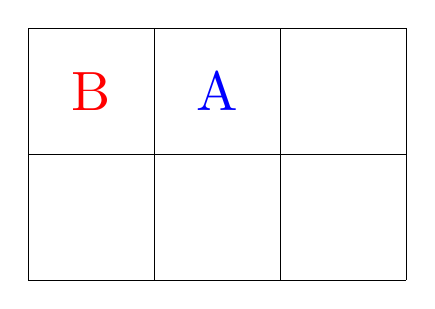
\begin{tikzpicture}[scale = 0.8]
                \draw (-3,2) -- (3,2);
                \draw (-3,-2) -- (3,-2);
                \draw (-3,0) -- (3,0);
                \draw (-3,-2) -- (-3,2);
                \draw (-1,-2) -- (-1,2);
                \draw (1,-2) -- (1,2);
                \draw (3,-2) -- (3,2);
                \node[red, scale = 2] (B) at (-2,1) {B};
                \node[blue, scale = 2] (A) at (0,1) {A};
            \end{tikzpicture}
            \qquad
            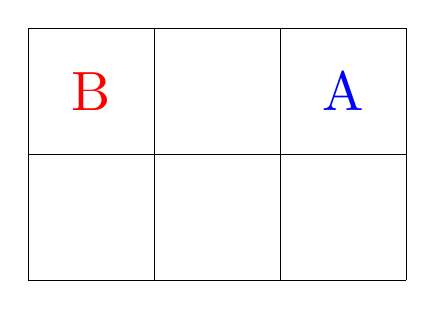
\begin{tikzpicture}[scale = 0.8]
                \draw (-3,2) -- (3,2);
                \draw (-3,-2) -- (3,-2);
                \draw (-3,0) -- (3,0);
                \draw (-3,-2) -- (-3,2);
                \draw (-1,-2) -- (-1,2);
                \draw (1,-2) -- (1,2);
                \draw (3,-2) -- (3,2);
                \node[red, scale = 2] (B) at (-2,1) {B};
                \node[blue, scale = 2] (A) at (2,1) {A};
            \end{tikzpicture}
        \end{center}
    
        \item 
    
        Describe what additional information the groupoid holds over the equivalence classes of configurations up to moves.
        
    \end{enumerate}
\end{Exercise}

\begin{Exercise}
    For an (associative and unital) ring $ R $ let $ B R $ be the category associated to the multiplicative monoid of $ R $.
    Show that there is an isomorphism of categories $ \psi \colon \Mod_R \to \Fun_{ \mathbb{ Z } } ( ( B R )^{ \op } , \Ab ) $ relating the category of right $ R $-modules into the category of '$ \mathbb{ Z } $-linear presheaves over $ B M $', i.e. contravariant $ \mathbb{ Z } $-linear functors from $ B R $ to the category of abelian groups $ \Ab $.
\end{Exercise}


\begin{Exercise}
    Let $ R $ be a ring and let $ \prescript{  }{ R }{ R }_R$ be $ R $ viewed as an $ R $-$ R $-bimodule.
    
    \begin{enumerate}[label=(\alph*)]
    
        \item 
        Show that for any $ R $-$ R $-bimodule $ N $ and any $ M \in \mod_R $ that $ \Hom_{ \mod R } ( N , M ) $ carries the structure of a right $ R $-module via $ ( f r ) ( x ) \coloneqq f ( r x ) $. 
        Deduce that $ N $ induces a functor
        \[
            \Hom_{\mod R } ( N , - ) \colon \mod R \to \mod R.
        \]
        
        \item 
        
        Show that there is an isomorphism of functors $ \Hom_{ \mod R } ( \prescript{}{ R }{ R }_R , - ) \cong \id_{ \mod R } $ given by evaluation at $ 1 \in R $.
    \end{enumerate}
\end{Exercise}

\begin{Exercise}
    Consider four sets $ A , B , C $ and $ E $ and assume that $ A , B \subseteq C $ with the inclusions $ \iota_A $ and $ \iota_B $.
    
    \begin{enumerate}[label=(\alph*)]
        \item 
        Show that for any two maps $ \phi_A \colon E \to A $ and $ \phi_B \colon E  \to B $ such that $ \iota_A \circ \phi_A = \iota_B \circ \phi_B $ there is a unique map $ \phi \colon E \to A \cap B $ such that $ \phi_A = i_A \circ \phi $ and $ \phi_B = i_B \circ \phi $ for $ i_A $ and $ i_B $ the respective inclusions of $ A \cap B $. 
        \[
        \begin{tikzcd}
            E 
            \ar[rd, dashed, " \exists ! \phi" ]
            \ar[rrd, bend left, " \phi_A" ]
            \ar[rdd, bend right, " \phi_B" ']
            \\
            &
            A \cap B
            \ar[r , " i_A " ]
            \ar[d , " i_B " ]
            &
            A
            \ar[ d , " \iota_A" ]
            \\
            &
            B
            \ar[r, " \iota_B " ]
            &
            C
        \end{tikzcd}
        \]
    
        \item 
        Give an example of two maps $ f_A \colon A \to D $ and $ f_B \colon B \to D $ such that $ A \cap B $ does not have the above property for $ f_A $ and $ f_B $ instead of $ \iota_A $ and $ \iota_B $.
    
        \item 
        Show that in this more genral setting that
        \[
            A \times_D B \coloneqq \{ ( a, b ) \in A \times B \mid f_A ( a ) = f_B ( b ) \}
        \]
        with the canonical projections $ p_A, p_B$ satisfying the universal property from before.
        \[
        \begin{tikzcd}
            E 
            \ar[rd, dashed, " \exists ! \phi" ]
            \ar[rrd, bend left, " \phi_A" ]
            \ar[rdd, bend right, " \phi_B" ']
            \\
            &
            A \times_D B
            \ar[r , " p_A " ]
            \ar[d , " p_B " ]
            &
            A
            \ar[ d , " f_A" ]
            \\
            &
            B
            \ar[r, " f_B " ]
            &
            D
        \end{tikzcd}
        \]
    
        \item 
        What is the relation between $ A \cap B $ and $ A \times_C B$ for part (a)?
    \end{enumerate}
\end{Exercise}
    



\section{Limits and Colimits}

For references for this section see \cite[Sections 5.1 \& 5.2 \& 5.3]{LeinBasi2014}.

Let $D$ be a small category, $\mathcal{C}$ be a category and $F \colon D \to \mathcal{C}$ a functor (a $D$-shaped diagram in $\mathcal{C}$).
For example let $D$ be given by
\[
10\xrightarrow{g}11\xleftarrow{f}01
\]
and let $F\colon D \to \mathcal{C}$ be a functor. We get a diagram
\[
F(10)\xrightarrow{F(g)}F(11)\xleftarrow{F(f)}F(01).
\]

\begin{defi}
    A \underline{cone over $F$} is a pair $(X , ( \phi_a)_{a\in A})$ consisting of 
    \begin{enumerate}
        \item 
        $X \in \mathcal{C},$
        \item 
        $(\phi_a\colon X \to F(a) \mid a \in A,$
    \end{enumerate}
    such that $\forall u \colon a \to b$ in $\mathcal{A}$
    \begin{tikzcd}
        &
        X
        \arrow[rd, "\phi_b"]
        \arrow[ld, "\phi_a"']
        &
        \\
        F(a)
        \arrow[rr, "F(u)"']
        &
        &
        F(b)
    \end{tikzcd}
    And $\phi_b=F(u) \circ \phi_a$.
    Cones form a category $\mathcal{C}/F$ with morphisms given by 
    \[
    f\colon(X,(\phi_a)_{a\in A}) \to (Y, (\sigma_a)_{a \in A})
    \]
    given by $f \colon  X \to Y$ such that for all $a \in A$
    \[
    \begin{tikzcd}
        X
        \arrow[rd, "\phi_a"']
        \arrow[rr,"f"]
        &
        &
        Y
        \arrow[ld,"\sigma_a"]
        \\
        &
        F(a)
    \end{tikzcd}
    \]
    A \underline{limit (cone)} of $F$ is a final object in $\mathcal{C}/F$.
    Explicitely $(\lim F, (\sigma_a)_{a \in A})$ is a limit of $F$ if for all cones $( X , (\phi_a)_{a\in A})$, there exists a unique $f \colon X \to \lim F$ in $\mathcal{C}$ such that for all $a \in A$ the following diagram commutes:
    \[
    \begin{tikzcd}
        X 
        \arrow[rd , "\phi_a"']
        \arrow[rr, "f"]
        &
        &
        \lim F
        \arrow[ld, "\phi_a"]
        \\
        &
        F(a)
        &
    \end{tikzcd}
    \]
\end{defi}

\begin{exmp}
    Let $A=\phi$ and $F\colon \phi \to \mathcal{C}$. 
    A limit is an object $\mathds{1} \in \mathcal{C}$ such that for all $X \in \mathcal{C}$ there exists a unique $f \colon X \to \mathds{1}$ that is $\mathds{1}$ is a final object in $\mathcal{C}$.
\end{exmp}

\begin{exmp}
    Let $A = \{ \text{\textcircled{1}} , \text{\textcircled{2}} \} \xrightarrow{F} \mathcal{C}$ be a functor the limit cone in $\mathcal{C}$ is given by the product, that is a cone $(Y, \pi_i)$ in $\mathcal{C}$.
    \[
    \begin{tikzcd}
        &
        &
        F(2)
        \\
        X
        \arrow[rru, bend left, "\phi_2"]
        \arrow[rrd, bend right, "\phi_1"']
        \arrow[r, "\exists !"]
        &
        Y
        \arrow[ru, "\pi_2"']
        \arrow[rd, "\pi_1"]
        &
        \\
        &
        &
        F(1)
    \end{tikzcd}
    \]
\end{exmp}

Lecture 17.10

If $(X , \overline{\rho}) = \overline{X}$ and $(Y , \overline{\sigma})=\overline{Y}$ are limits of $F \colon A \to \mathcal{C}$.
Then there is a unique isomorphism of cones $\overline{X} \to \overline{Y}$.
It is enough to prove the statement for final objects, by definition of the limit cone.
Let $X,Y \in \mathcal{D}$ be final objects.
Then there exists a unique morphism $f \colon X \to Y$ in $\mathcal{D}$ since $Y$ is final.
Then there exists a unique morphism $f \colon Y \to X$ in $\mathcal{D}$ since $X$ is final.
But then $g \circ f (X) = X$ must be $g \circ f = \id_X$ since $X$ is \underline{final}.

\begin{prop}
    Suppose that $(\lim F , \overline{\sigma} )$ is a limit of $F \colon \mathcal{A} \to \mathcal{C}$ and $f \colon X \to \lim F$ is an isomorphism.
    Then $(X ,(\sigma_a f\colon X \to F(a)) a \in \mathcal{A})$ is a limit cone.
\end{prop}

\begin{proof}
    For all $u \colon a \to b$ in $A$, we have get the following commutative diagram: 
    \[
    \begin{tikzcd}
        &
        X
        \arrow[ld,"\sigma_a \circ f"']
        \arrow[rd,"\sigma_b \circ f"]
        &
        \\
        F(a)
        \arrow[rr, "F(u)"']
        &
        &
        F(b)
    \end{tikzcd}
    \]
    which means that 
    \[
    F(u) \circ (\sigma_a \circ f) =\sigma_b \circ f.
    \]
    Thus $(X,(\sigma_a \circ f)_{a \in A})$ is indeed a cone and $f \colon (X, ( \sigma \circ f )_{a \in A}) \to (\lim_A F , \overline{\sigma})$ is an isomorphism of cones since $f$ is an isomorphism and since 
    \[
    \begin{tikzcd}
        X
        \arrow[rr,"f"]
        \arrow[rd,"\sigma_a \circ f"']
        &
        &
        \lim_A F
        \arrow[ld, "\sigma_a"]
        \\
        &
        F(a)
        &
    \end{tikzcd}
    \]
    commutes for all $a$ in $A$.
\end{proof}

\begin{defi/prop}
    A category $\mathcal{C}$ is complete if for all small categories $A$ and functors $F:A \to \mathcal{C}$ a limit of $F$ exists.
    The category $\Set$ is complete.
\end{defi/prop}

\begin{proof}
    Let $A$ be a small category and $F\colon A  \to \Set$ a diagram.
    Let 
    \[
    \lim_A F \coloneqq \{ \Bar{X} = (X_a)_{a \in A} \in \prod_{a \in A} F(a) \mid \forall u \colon a \to b \text{ in } A, F(u)(X_a)=X_b\}
    \]
    This this is a subset of a product, it comes with projections.
    We get that $(\lim_A F, (\pi_a:\Bar{X} \to X_a)_{a\in A})$ is a cone over $F$ since for all morphisms $u \colon a \to b$ in $A$ we get that the following diagram 
    \[
    \begin{tikzcd}
        &
        \lim_A F
        \arrow[ld,"\pi_a"']
        \arrow[rd,"\pi_b"]
        &
        \\
        F(a)
        \arrow[rr,"F(a)"']
        &
        &
        F(b)
    \end{tikzcd}
    \]
    equates to 
    \[
    \begin{tikzcd}
        &
        \Bar{X}
        \arrow[ld,"\pi_a"']
        \arrow[rd,"\pi_b"]
        &
        \\
        X_a
        \arrow[rr,"F(u)(X_a)"']
        &
        &
        X_b
    \end{tikzcd}
    \]
    Now let $(X, (\rho_a \colon X \to F(a) \mid a \in A))$ be another cone over $F$.
    Define $\Bar{\rho}: X \to \prod_{a \in A} F(a)$ by $x \mapsto (\rho_a(x))_{a \in A}$.
    Notice that $\Bar{\rho}$ factors through $\lim_A F \subseteq \prod_{a \in A} F(a)$ since for all $x \in X$ and for all morphisms $u\colon a \to b$, we have that $F(u)(\rho_a(x))=\rho_b(x)$ since the following diagram commutes
    \[
        \begin{tikzcd}
            &
            X
            \arrow[ld, "\rho_a"']
            \arrow[rd, "\rho_b"]
            &
            \\
            F(a)
            \arrow[rr, "F(u)"']
            &
            &
            F(b)
        \end{tikzcd}
    \]
    Thus $\Bar{\rho} \to \lim_A F$ is well defined.
    Observe that $\Bar{\rho}$ is actually a morphism of cones, since 
    \[
    \begin{tikzcd}
        X
        \arrow[rr, "\Bar{\rho}"]
        \arrow[rd, "\rho_b"']
        &
        &
        \lim F
        \arrow[ld, "\pi_b"]
        \\
        &
        F(b)
        &
    \end{tikzcd}
    \qquad
    \begin{tikzcd}
        x
        \arrow[rr , mapsto , "\Bar{\rho}"]
        \arrow[rd , mapsto]
        &
        &
        (\rho_a(x))_{a \in A}
        \arrow[ld, mapsto , "\pi_b"]
        \\
        &
        \rho_b(x)
        &
    \end{tikzcd}
    \]
    Finally if $f\colon ( X , ( \rho_a )_{a \in A}) \to ( \lim_A F , (\pi_a)_{a \in A})$ is a morphism of cones, then (by definition) we get for all $a \in A$ 
    \[
    \begin{tikzcd}
        X
        \arrow[rr, "f"]
        \arrow[rd, "\rho_a"']
        &
        &
        \lim_A F
        \arrow[ld, "\pi_a"]
        \\
        &
        F(a)
        &
    \end{tikzcd}
    \]
    that is for all $x \in X$ we get $\pi_a(f(x)) = \rho_a(x)$, so $f= \Bar{\rho}$.
\end{proof}

\begin{defi}
    A functor $G$ \underline{preserves limits of shape $A$} if for all functors $F\colon A \to \mathcal{C}$, $G$ sends limit cones of $F$ to limit cones of $G \circ F$. 
    A functor $G$ preserves limits if for all small categories $A$ we have that $G$ preserves limits of shape $A$.
\end{defi}

\begin{rmk}
    Consider the example of the covariant $\Hom$-functor.
     Let $F \colon  A \to \mathcal{C}$ and $X\in \mathcal{C}$.
     Consider the covariant functor $\Hom_{\mathcal{C}}(X,-) \colon \mathcal{C} \to \Set$ and a limit $\sigma_a\colon \lim_A F \to F(a)$.
     We can put these together to obtain a cone $\Hom_{\mathcal{C}}(X, \sigma_a) \colon \Hom_{\mathcal{C}}(X, \lim F) \xrightarrow{\sigma_a \circ ?=(\sigma_a)_*} \Hom_{\mathcal{C}}(X,F(a))$.
\end{rmk}

\begin{thm}
\label{covariant_hom_preserves_limits}
    The functor $\Hom_{\mathcal{C}}(X,-) \colon \mathcal{C} \to \Set$ preserves limits.
\end{thm}

\begin{proof}
    Consider the map
    \[
    \begin{tikzcd}
        \Hom_{\mathcal{C}}(X, \lim_A F) 
        \arrow[r, "\phi"]
        &
        \lim_{a \in A} \Hom_{\mathcal{C}} ( X, F(a)) 
        \\
        (X \xrightarrow{f} \lim_A F) 
        \arrow[r, mapsto]
        &
        (\sigma_a  \circ f\colon X \xrightarrow{f} \lim_A F \xrightarrow{\sigma_a} F(a))_{a \in A}
    \end{tikzcd}
    \]
    This is a morphism of cones, now we need to show it is bijective.
    For injectivity, assume there are two morphisms $ X \underset{g}{\overset{f}{{\rightrightarrows}}} \lim_A F$ such that $\phi(f)=\phi(g)$.
    Then for all $a \in A$ we get that $\sigma_a \circ f = \sigma_a \circ g$ and for all morphisms $a \to b$
    \[
    \begin{tikzcd}
        &
        X
        \arrow[rrrr, shift left , "f"]
        \arrow[rrrr, shift right, "g"']
        \arrow[ld]
        \arrow[rd]
        &
        &
        &
        &
        \lim_A F
        \arrow[ld, "\sigma_a"']
        \arrow[rd, "\sigma_b"]
        &
        \\
        F(a)
        \arrow[rr, "F(u)"]
        &
        &
        F(b)
        &
        &
        F(a)
        \arrow[rr ,"F(u)"]
        &
        &
        F(b)
    \end{tikzcd}
    \]
    which means $f$ and $g$ are morphisms of cones, but by the uniqueness of a morphism into a limit, such that the above commutes, we get that $f=g$.
    For the surjectivity, let $(f_a \colon X \to F(a))_{a\in A}$ be morphism indexed by $A$ and take $\lim_{a \in A} \Hom( X, F(a))$.
    This means that for all morphism $u \colon a  \to  b$ in $A$, we have that $\Hom_{\mathcal{C}}(X,F(u))(f_a)=f_b$,
    so that $(X, (f_a \colon \to F(a))_{a \in A})$ is a cone over $F$.
    Thus there exists a unique morphism into the limit cone $\psi: (X,(f_a)_{a \in A}) \to ( \lim_A F, (\sigma_a)_{a \in A})$, where $\sigma_a \circ \psi =f_a$ that is $\phi(f)= (f_a)_{a \in A}$.
\end{proof}

\begin{thm}
    The Yoneda embedding $\mu \colon \mathcal{A} \to \widehat{A} = \Fun ( \mathcal{A}^{\op}, \Set )$ preserves limits.
\end{thm}

\begin{proof}
    The proof is just an application of $\cref{covariant_hom_preserves_limits}$ to the Yoneda embedding from $\cref{yoneda_embedding}$.
\end{proof}

\subsection{Exercise}

\begin{Exercise}
    Show that two objects $ a , b \in A $ in a category $ A $ are isomorphic if and only if their respresentable presheaves $ \Hom_A ( - , a ) $ and $ \Hom_A ( -, b ) $ are isomorphic in $ \widehat{ A } $.
\end{Exercise}

\begin{Exercise}
    Consider a functor $ F \colon A  \to \mathcal{ C } $ from a small category $A$.
    
    \begin{enumerate}
        \item 
        Show that if $ A $ is an initial object $ \emptyset $, then the limit of $ F $ exists.
    
        \item 
        Show that if $ A $ has a final object $ e $, then the colimit of $ F $ exists.
    \end{enumerate}
\end{Exercise}

\begin{Exercise}
    Let $ F \colon A \to \set $ be a functor from a small category to the category of sets.
    Recall that we have shown in the lecture that the limit of $ F $ exists and is given by 
    \[
        \lim_A F \coloneqq \bigg\{ x \in \prod_{ a \in A } F ( a ) \mid \forall u \colon a \to b \quad F ( u ) ( x_a ) = x_b \bigg\}
    \]
    together with the canonical projections.
    
    \begin{enumerate}[label=(\alph*)]
        \item 
        Show that the inclusion $ \lim_A F \subseteq \prod_{ a \in A } F ( a ) $ exhibits $ \lim_A F $ as the equalizer (= limit of the following diagram)
        \[
        \begin{tikzcd}
            \prod_{ a \in A } F ( a ) 
            \ar[r , shift left, " \phi "]
            \ar[r , shift right, " \psi "']
            &
            \prod_{ \substack{ u \colon s \to t \\ \text{ in } A} } F ( t )
        \end{tikzcd}
        \]
        where $ \phi ( x )_u = F ( u ) ( x_{ s ( u ) } ) $ and $ \psi ( x )_u = x_{ t ( u ) }$.
    
        \item 
        Let $ \coprod $ denote the disjoint union of sets. 
        Assume that the coequalizer ( = colimit of the following diagram ) 
        \[
        \begin{tikzcd}
            \coprod_{ \substack{ u \colon s \to t \\ \text{ in } A} } F ( t )
            \ar[r , shift left, " \phi "]
            \ar[r , shift right, " \psi "']
            &
            \coprod_{ a \in A } F ( a ) 
        \end{tikzcd}    
        \]
        exists where for $ y \in F ( s ( v ) ) \subseteq \coprod_{ \substack{ u \colon s \to t \\ \text{ in } A} } F ( t ) $ we have $ \phi ( y ) = F ( v ) ( y ) \in F ( t ( v ) ) \subseteq \coprod_{ a \in A } F ( a ) $ and $ \psi ( y ) = y \in F ( s ( v ) ) \subseteq \coprod_{ a \in A } F ( a ) $. Show that it is a colimit of $ F $ with the canonical maps fro $ F ( a ) $.
    \end{enumerate}
\end{Exercise}

\begin{Exercise}
    \begin{enumerate}[label=(\alph*)]
        \item 
        Show that the disjoint union of sets defines a coproduct in the category of sets, i.e. show that for every family of sets $ ( U_i )_{ i \in I } $ their disjoint union $\coprod_{ i \in I } U_i $ together with the canonical inclusion $ U_j \subseteq \coprod_{ i \in I } U_i $ is the colimit of the functor $ U \colon I \to \Set $ assigning to each $ i \in I $ the set $ U_i $.
        Here $ I $ is some indexing set.
    
        \item 
        Show that any coequalizer (= colimit of the following diagram ) 
        \[
        \begin{tikzcd}
            U 
            \ar[r, shift left, " \phi "]
            \ar[r, shift right, " \psi "']
            & 
            V
        \end{tikzcd}
        \]
        exists in Set by considering the smallest equivalence relation on $ V $ such that $ v \sim v' $ whenever there is some $ u \in U $ such that $ \phi ( u ) $ and $ \psi ( u ) = v' $.
    
        \item 
        Conclude using Exercise 2.3 that Set is cocomplete, i.e. every small colimit exists.
    \end{enumerate}
\end{Exercise}   
\section{Adjunctions}

Lecture 22.10

For references for this section see \cite[Sections 2.1 \& 2.2 \& 2.3 \& 6.1]{LeinBasi2014}.

Everytime you encounter some free object, in the sense that it is freely generated from some other object of some other category, like a free group on some set, you are most likely going to use the properties of the object stemming from an adjunction.

\begin{defi}
    \begin{tikzcd}
        L \colon  \mathcal{C} 
        \arrow[r, shift left]
        &
        \mathcal{D} \colon R
        \arrow[l, shift left]
    \end{tikzcd}
    An adjunction $L \dashv R$ is a natural isomorphism $\phi_{c,d} \colon \Hom_\mathcal{D} (Lc,d) \isomorphism \Hom_\mathcal{C}(c,Rd)$ of functors $\mathcal{C}^{\op} \times \mathcal{D} \to \Set$.
    \[
    \begin{tikzcd}
        \mathcal{C}^{\op} \times \mathcal{D}
        \arrow[bend left]{rr}[above]{\Hom_{\mathcal{D}}(L(-),-)}[below,name=U]{}
        \arrow[bend right]{rr}[below]{\Hom_{\mathcal{C}}(-,R(-))}[above,name=D]{}
        \arrow[Rightarrow, from=U, to=D, right, "\phi"]
        &
        &
        \Set
    \end{tikzcd}
    \]
    That is explicitely, we have commutative squares for all pairs of morphisms:
    \[
    \begin{tikzcd}
        (c,d) 
        \arrow[d, shift left, "\id_d"]
        &
        \Hom_{\mathcal{D}}(Lc,d) 
        \arrow[r, "\phi_{c,d}"]
        \arrow[d, "g \circ ?"']
        &
        \Hom_{\mathcal{C}}(c,Rd)
        \arrow[d, "R(g) \circ ?"]
        \\
        (c',d)
        \arrow[u, shift left , "f"]
        &
        \Hom(Lc,d')
        \arrow[r, "\phi_{c,d'}"']
        &
        \Hom_{\mathcal{C}}(c , Rd')
    \end{tikzcd}
    \]
    which means that for all $f \colon Lc \to d$ and all $g \colon d \to d'$ we have that $R(g) \circ \Bar{f} = \overline{g \circ f}$, where the closure operator denotes the image of an element under $\phi$
    \[
    \begin{tikzcd}
        (c,d) 
        \arrow[d, shift left, "\id_g"]
        &
        \Hom_{\mathcal{D}}(Lc,d) 
        \arrow[r, "\phi_{c,d}"]
        \arrow[d, "? \circ Lf"']
        &
        \Hom_{\mathcal{C}}(c,Rd)
        \arrow[l, "\Bar{(-)}"]
        \arrow[d, "? \circ f ?"]
        \\
        (c',d)
        \arrow[u, shift left , "f"]
        &
        \Hom(Lc',d)
        &
        \Hom_{\mathcal{C}}(c' , Rd)
        \arrow[l, "\Bar{(-)}"]
    \end{tikzcd}
    \]
    which means that for all $k \colon c \to Rd$ and all $f \colon c' \to c$ we have that $\Bar{k} \circ Lf = \overline{k \circ f}$.
\end{defi}

\begin{rmk}
    For $c \in \mathcal{C}$ consider $\eta_c$ given as follows
    \[
    \begin{tikzcd}
        \Hom_{\mathcal{D}}(Lc,Lc)
        \arrow[r ,"\sim"]
        &
        \Hom_{\mathcal{C}}(c,RLc)
        \\
        \id_{Lc}
        \arrow[r , mapsto]
        &
        \eta_c \coloneqq \overline{\id_{Lc}}
    \end{tikzcd}
    \]
    as well as for any $d \in \mathcal{D}$ consider $\epsilon_d$ given as follows
    \[
    \begin{tikzcd}
        \Hom_{\mathcal{C}}(Rc,Rc)
        \arrow[r ,"\sim"]
        &
        \Hom_{\mathcal{D}}(LRd , d )
        \\
        \id_{Rc}
        \arrow[r , mapsto]
        &
        \epsilon_d \coloneqq \overline{\id_{Rd}}
    \end{tikzcd}
    \]
\end{rmk}

\begin{prop}
    Notice that $\eta=(\eta_c \colon c \to RLc \mid c \in \mathcal{C})$ is a natural transformation $\eta \colon \mathds{1}_{\mathcal{C}} \ RL $ we call this the \underline{unit} of the adjunction and similarly $\epsilon=(\epsilon_c \colon c \to LRd \mid d \in \mathcal{C})$ is a natural transformation $\epsilon\colon LR  \to \mathds{1}_{\mathcal{D}}$ and is a called the \underline{counit} of the adjunction.
\end{prop}

\begin{proof}
    Consider the following square:
    \[
    \begin{tikzcd}
        c 
        \arrow[d, "f"]
        &
        c
        \arrow[r, "\eta_{\mathcal{C}}"]
        \arrow[d, "f"']
        &
        RLc
        \arrow[d, "RLf"]
        \\
        c'
        &
        c'
        \arrow[r, "\eta_{c'}"']
        &
        c'
    \end{tikzcd}
    \]
    and the resulting equation
    \begin{align}
        & RLf \circ \eta_c 
        = \eta_c' \circ f
        \\
        \iff& \overline{RLf \circ \eta_c} 
        = \overline{\eta_{c'} \circ f}
        \\
        \iff& \overline{\overline{Lf}}
        =\overline{\id_{c'} \circ Lf} 
        \\
        \iff&
        Lf = \id_f \circ Lf
    \end{align}
\end{proof}

\begin{prop}
    The unit $\eta \colon \mathds{1}_{\mathcal{C}} \Rightarrow RL$ aand the counit $\epsilon \colon LR \Rightarrow \mathds{1}_{\mathcal{D}}$ satisfy the triangle identities:
    \[
    \begin{tikzcd}
        &
        LRLc
        \arrow[rd, "\epsilon_{Lc}"]
        &
        \\
        Lc
        \arrow[ru, "L(\eta_c)"]
        \arrow[rr, "\id_{Lc}"']
        &
        &
        Lc
    \end{tikzcd}
    \qquad
    \begin{tikzcd}
        &
        RLRd
        \arrow[rd, "R(\epsilon_{d})"]
        &
        \\
        Rd
        \arrow[ru, "\eta_{Rd}"]
        \arrow[rr, "\id_{Rd}"']
        &
        &
        Rd
    \end{tikzcd}
    \]
    For all objects $c\in \mathcal{C}$ and $d \in \mathcal{D}$.
\end{prop}

\begin{proof}
    If we take the triangle for the unit above and apply the bar-operator we obtain the following
    \[
    \begin{tikzcd}
        &
        LRLc
        \arrow[rd, "\epsilon_{Lc}"]
        &
        \\
        Lc
        \arrow[ru, "L(\eta_c)"]
        \arrow[rr, "\id_{Lc}"']
        &
        &
        Lc  
    \end{tikzcd}
    \xleftrightarrow{\overline{(-)}}
    \begin{tikzcd}
        &
        RLc
        \arrow[rd, "\id_{RLc}"]
        &
        \\
        c
        \arrow[ru, "\eta_c"]
        \arrow[rr, "\overline{\id_{c}}=\eta_c"']
        &
        &
        RLc
    \end{tikzcd}
    \]
    The second triangle clearly commutes, the argument for the counit is analogous.
\end{proof}

\begin{prop}
    Let \begin{tikzcd}
        L \colon  \mathcal{C} 
        \arrow[r, shift left]
        &
        \mathcal{D} \colon R
        \arrow[l, shift left]
    \end{tikzcd}
    be two functors between categories and suppose there exist natural transformations $\eta \colon \mathds{1}_{\mathcal{C}} \Rightarrow RL$ and $\eta\colon LR \Rightarrow \mathds{1}_{\mathcal{D}}$ that satisfy the triangle identities.
    Then the following defines an adjunction $L \dashv R$
    \[
    \begin{tikzcd}
        \phi \colon \Hom_{\mathcal{D}}(Lc,d)
        \arrow[r, shift left]
        &
        \Hom_{\mathcal{C}}(c,Rd) \colon \psi
        \arrow[l, shift left]
        \\
        Lc \xrightarrow{g} d
        \arrow[r, mapsto ,shift left]
        &
        R(g)\circ \eta_c
        \arrow[l, mapsto ,shift left]
    \end{tikzcd}
    \]
\end{prop}

\begin{proof}
    For $g \colon Lc \to d$ we have that 
    \[
        g=(\psi\circ\phi)(g) = \psi(R(g) \circ \eta_c) = \epsilon_d \circ LR(g) \circ L(\eta_c)
    \]
    Now we have the following the diagram
    \[
    \begin{tikzcd}
        &
        LRLc
        \arrow[rd, "\epsilon_{Lc}"]
        \arrow[rr, "LRg"]
        &
        &
        LRd
        \arrow[rd, "\epsilon_d"]
        \\
        Lc 
        \arrow[ru,"L(\eta_c)"]
        \arrow[rr,"\id_{Lc}"']
        &
        &
        Lc 
        \arrow[rr,"g"']
        &
        &
        d
    \end{tikzcd}
    \]
    The triangle commutes due to the triangle identities and the square commutes by the naturality of the counit. thus the whole diagram commutes, which means that $\psi$ is an inverse to $\phi$ which yields the statement.    
\end{proof}

\begin{defi}
    For $c \in \mathcal{C}$ and $R\colon \mathcal{D}\to\mathcal{C}$ a functor, define the category $c/R$ with objects given by tuples $(c,f)$
    where $f\colon c \to R(d)$ is a morphism for some $d\in \mathcal{D}$ and morphisms are given by 
    \[
    \begin{tikzcd}
        d \in \mathcal{D} 
        \arrow[d,"g"]
        &
        c
        \arrow[r,"f"]
        \arrow[d, equal]
        &
        Rd
        \arrow[d,"R(g)"]
        \\
        d' \in \mathcal{D}
        &
        c
        \arrow[r,"f'"']
        &
        Rd'
    \end{tikzcd}
    \]
    Dually for $L \colon \mathcal{C} \to \mathcal{D}$ and $d \in \mathcal{D}$ we define $L/d$ as tuples $(d,g)$ where $g\colon Lc \to g$ is a morphism and morphisms are given by 
    \[
    \begin{tikzcd}
        c \in \mathcal{C} 
        \arrow[d,"f"]
        &
        Lc
        \arrow[r,"g"]
        \arrow[d, "Lf"']
        &
        d
        \arrow[d, equal]
        \\
        c' \in \mathcal{C}
        &
        Lc'
        \arrow[r,"g'"']
        &
        d
    \end{tikzcd}
    \]
    Notice that given an adjunction $ L \dashv R$ we have that $\forall c \in \mathcal{C} (c,c \xrightarrow{\eta_c} RLc)$ is in $c/R$ and $\forall \in \mathcal{D}(d, LRd \xrightarrow{\epsilon_d} d)$ is in $L/d$.
\end{defi}

\begin{prop}
\label{initial_final_comma_category}
    The object $(c,c \xrightarrow{\eta_c} RLc)$ is initial in $c/R$ and
    $(d, LRd \xrightarrow{\epsilon_d} d)$ is final in $L/d$.
\end{prop}

\begin{proof}
    Consider the following commutative triangle
        \[
        \begin{tikzcd}
            c 
            \arrow[r, " \eta_c "] 
            \arrow[rd, "\overline{\overline{f}}=f"']
            &
            RLc
            \arrow[d,"R(\overline{f})"]
            \\
            &
            Rd
        \end{tikzcd}
        \]
    where $\overline{\overline{f}}=\overline{R(\overline{f})\circ \eta_c}$. 
    Thus the morphism $f$ of the object $(c,f)$ uniquely determines the morphism $R(\overline{f})$. 
    The argument for final object is dual to this one.
\end{proof}

Lecture 24.10

\begin{prop}
    Let 
    \[
    \begin{tikzcd}
        \mathcal{C}
        \arrow[r, shift left, "L_1"]
        &
        \mathcal{D}
        \arrow[l, shift left, "R_1"]
        \arrow[r, shift left, "L_2"]
        &
        \mathcal{E}
        \arrow[l, shift left, "R_2"]
    \end{tikzcd}
    \]
    be adjunctions then their composition
    \[
    \begin{tikzcd}
        \mathcal{C}
        \arrow[r, shift left, "L_1\circ L_2"]
        &
        \mathcal{D}
        \arrow[l, shift left, "R_1\circ R_2"]
    \end{tikzcd}
    \]
    is an adjunction as well.
\end{prop}

\begin{proof}
Consider the following transformations, given by the adjunction isomorphisms
    \[
    \Hom_{\mathcal{E}}(L_2L_1c,e) \isomorphism \Hom_{\mathcal{D}}(L_1c,R_2e) \isomorphism \Hom_{\mathcal{C}}(c,R_1R_2e)
    \]
\end{proof}

\begin{rmk}
    Given an adjunction 
    \[
    \begin{tikzcd}
        \mathcal{C}
        \arrow[r, shift left, "L"]
        &
        \mathcal{D}
        \arrow[l, shift left, "R"]
    \end{tikzcd}
    \]
    then the following is an adjunction as well
    \[
    \begin{tikzcd}
        \mathcal{C^{\op}}
        \arrow[r, shift left, "L^{\op}"]
        &
        \mathcal{D^{\op}}
        \arrow[l, shift left, "R^{\op}"]
    \end{tikzcd}
    \]
    and the unit $\eta_c\colon c \to RLc$ in $\mathcal{C}$ corresponds to the counit $c \xleftarrow{}RLc$ in $\mathcal{C}^{\op}$
\end{rmk}

\begin{prop}
    Let $L_1 ; L_2 \colon \mathcal{C} \to  \mathcal{D}$ and $\mathcal{C} \xleftarrow{}\mathcal{D}:R$ be functors.
    Suppose that $L_1 \dashv R$ and $L_2 \dashv R$ are adjunctions, then it follows that $L_1 \cong L_2$.
\end{prop}

\begin{proof}
    We need to construct a natural isomorphism $\phi \colon L_1 \isomorphism L_2$.
    Let $\eta^{(1)}\colon \mathds{1} \to RL_1$ and $\eta^{(2)} \colon \mathds{1}_{\mathcal{C}} \to RL_2$.
    By the uniqueness of initial objects in $c/R$, for $c \in \mathcal{C}$ \cref{initial_final_comma_category} we obtain 
    \[
    \begin{tikzcd}
        &
        c
        \arrow[ld, "\eta^{(1)}_c"']
        \arrow[d, "\eta^{(2)}_c"]
        \arrow[rd, "\eta^{(1)}_c"]
        &
        \\
        RL_1c
        \arrow[r, dashed, "Rg"']
        &
        RL_2c
        \arrow[r, dashed, "Rh"']
        &
        RL_1c
    \end{tikzcd}
    \]
    By the uniqueness of a morphism out of an initial object we obtain for the composition that 
    $L_1c \xrightarrow{g}L_2c \xrightarrow{h}L_1c$ 
    is given by $h \circ g = \id_{L_1c}$. 
    Similarly one obtains $g \circ h = \id_{L_2c}$.
    Thus $g \eqqcolon U_c \colon L_1c \isomorphism L_2c$.
    We now have to check that $U_c$ is actually a natural transformation of functors. Consider the following diagram
    
    \[
    \begin{tikzcd}
        c 
        \arrow[d, "f"]
        &
        L_1c
        \arrow[r, "U_c"]
        \arrow[d, "L_1f"']
        &
        L_2c
        \arrow[d, "L_2f"]
        \\
        c'
        &
        L_1c'
        \arrow[r, "U_c'"']
        &
        L_2c'
    \end{tikzcd}
    \]
    apply $R$ to it 
    \[
    \begin{tikzcd}
        &
        c
        \arrow[dl, "\eta^{(1)}_c"']
        \arrow[dr, "\eta^{(2)}_c"]
        \arrow[dd, "f", pos=0.7]
        &
        \\
        RL_1c
        \arrow[rr, crossing over, "R(U_c)", pos=0.3]
        \arrow[dd, "RL_1(f)"']
        &
        &
        RL_2c
        \arrow[dd,"RL_2(f)"]
        \\
        &
        c'
        \arrow[ld, "\eta_{c'}^{(1)}"']
        \arrow[rd, "\eta_{c'}^{(2)}"]
        &
        \\
        RL_1c'
        \arrow[rr, "R(U_{c'})"]
        &
        &
        RL_2(c')
    \end{tikzcd}
    \]
    This yields the following equations
    \begin{align}
        R(U_{c'} \circ L_1(f)) \circ \eta^{(1)}_c
        &= R (U_{c'}) \circ \eta_{c'}^{(1)} \circ f
        \\
        &= \eta_{c'}^{(2)} \circ f
        \\
        &=RL_2(f) \circ \eta_c^{(2)}
        \\
        &=RL_2(f) \circ R(U_c) \circ \eta_c^{(1)}
        \\
        &=R(L_2(f) \circ U_c) \circ \eta_c^{(1)}
    \end{align}
    And thus results in the following commutative triangle 
    \[
    \begin{tikzcd}
        c 
        \arrow[rr, "\eta_c^{(1)}"]
        \ar[rrd, bend right, "\eta_{c'}^{(2)} \circ f"']
        &&
        RL_1c
        \dar[shift left, "R(L_2(f) \circ U_c)"]
        \dar[shift right, "R(U_{c'} \circ L_1(f))"']
        \\
        &&
        RL_2(c)
    \end{tikzcd}
    \]
    Both compositions give an initial object in $c/R$ by \cref{initial_final_comma_category}, thus by the uniqueness of an initial object they are equal in $c/R$ and thus $U_{c'} \circ L_1(f)=L_2(f) \circ U_c$.
\end{proof}

\begin{prop}
    Let $\begin{tikzcd}
        \mathcal{C}
        \arrow[r, shift left, "L"]
        &
        \mathcal{D}
        \arrow[l, shift left, "R"]
    \end{tikzcd}$
    be an adjunction then $L$ preserves colimits that exist in $\mathcal{C}$ and $R$ preserves limits that exist in $\mathcal{D}$.
\end{prop}

\begin{proof}
    Let $X\colon A \to \mathcal{C}$ be a diagram that admits a colimit in $\mathcal{C}$, $\colim X_a \in \mathcal{C}$ and $ a \in A$.
    \begin{align}
        \Hom_{\mathcal{D}}(L(\colim_{a \in A} X_a),d) 
        &\isomorphism \Hom_{\mathcal{C}}(\colim_{a \in A} X_a, Rd)
        \\
        &\isomorphism \lim_{a \in A} \Hom_{\mathcal{C}}(X_a,Rd)
        \\
        &\isomorphism \lim_{a \in A} \Hom_{\mathcal{C}}(LX_a,d)
        \\
    \end{align}
    This exhibits $L(\colim_{a \in A} X)$ as a colimit of $X\colon A \xrightarrow{X} \mathcal{C} \xrightarrow{L} \mathcal{D}$.
\end{proof}

Let $A$ be a small category and $\mathcal{C}$ a category.
Consider the functor $\const_A \colon \mathcal{C} \to \Fun(A , \mathcal{C})$
that maps each object of $\mathcal{C}$ to the functor $F_c(a)=c$ for all $a \in A$ and each morphism to $\id_c$.

\begin{prop}
    Suppose that there exists $L \colon \Fun(A,\mathcal{C}) \to \mathcal{C}$ a left adjoint to $\const_A$. 
    Then for all $X \colon A  \to \mathcal{C}$ the unit $\eta_X \colon X \to \const_A(LX)$ exhibits $LX$ as a colimit of $X$.
\end{prop}

\begin{proof}
    We know by \cref{initial_final_comma_category} that $\eta_X \colon X \to \const_A(LX)$ is initial in $X / \const_A$.
    Notice that the objects of $X/\const_A$ are pairs
    $(c \in \mathcal{C}, \rho \colon X \Rightarrow \const_A(c))$.
    Thus $\Bar{\rho} = ( \rho_a \colon X_a \to c \mid a \in A )$ is such that 
    \[
    \begin{tikzcd}
        a
        \arrow[d,"u"]
        &
        X_a 
        \arrow[r, "\rho_a"]
        \arrow[d, "X_u"']
        &
        c
        \arrow[d, "\id_c"]
        \\
        b
        &
        X_b
        \arrow[r, "\rho_b"]
        &
        c
    \end{tikzcd}
    \]
    Let furthermore $f\colon c \to c'$ be a morphism inducing a morphism in $X/\const_A$
    \[
    \begin{tikzcd}
        X 
        \arrow[r, Rightarrow, "\Bar{\rho}"]
        \arrow[d, equal]
        &
        \const_A(c)
        \arrow[d, "\const_A(f)"]
        \\
        X 
        \arrow[r, Rightarrow, "\Bar{\sigma}"]
        &
        \const_A(c')
    \end{tikzcd}
    \]
    given evaluated on objects $a \in A$ by 
    \[
    \begin{tikzcd}
        X_a
        \arrow[r, "\phi_a"]
        \arrow[rd, " \sigma_a"]
        \arrow[d, equal]
        &
        c
        \arrow[d, "f"] 
        \\
        X_a
        \arrow[r,"\sigma_a"']
        &
        c'
    \end{tikzcd}
    \]
    The two diagrams above tell us, that $c$ together with the $\phi_a$ is a cocone and combining this with the universality of the initial object, we obtain that $LX$ is a colimit.
\end{proof}

\begin{prop}
    Let $\mathcal{C} \xleftarrow{}\mathcal{D}:R$ be such that for all $c \in \mathcal{C}$ the functor $\Hom_{\mathcal{C}}(c,R(-))\colon \mathcal{D} \to \Set$ is corepresentable by an object $L(c) \in \mathcal{D}$ via $\phi_c \colon \Hom_{\mathcal{D}}(L(c),-) \isomorphism \Hom_{\mathcal{D}}(c,R(-))$.
    Then the association $c \mapsto L(c)$ can be promoted to a functor $L \colon \mathcal{C} \to \mathcal{D}$ that is adjoint to $R$ via $\phi$.
\end{prop}

\begin{proof}
    We need to define $L$ on morphisms.
    For $c \xrightarrow{f}c'$ in $\mathcal{C}$ consider the commutative square
    \[
    \begin{tikzcd}
        \Hom_{\mathcal{D}}(L(c),-)
        \arrow[r, "\phi_c"]
        &
        \Hom_{\mathcal{C}}(c,R(-))
        \\
        \Hom_{\mathcal{D}}(L(c'),-)
        \arrow[u, dashed, "L(f)^*"]
        \arrow[r, "\phi_{c'}"]
        &
        \Hom_{\mathcal{C}}(c',R(-))
        \arrow[u, "f^*"']
    \end{tikzcd}
    \]

    By Yoneda we obtain an object $d \in\mathcal{D}$ such that
    \[
    \begin{tikzcd}
        L(c)
        \arrow[d, "L(f)"']
        \arrow[rd]
        &
        \\
        L(c')
        \arrow[r]
        &
        d
    \end{tikzcd}
    \]
    Now we need to prove that this actually defines a functor $L\colon \mathcal{C} \to \mathcal{D}$.
    For $c \in \mathcal{C}$ we have that $L(\id_c)=\id_{L(c)}$ by construction.
    Let $c \xrightarrow{f}c' \xrightarrow{g}c''$ be in $\mathcal{C}$.
    \[
    \begin{tikzcd}
        \Hom_{\mathcal{D}}(L(c),-)
        \arrow[r, "\phi_c"]
        &
        \Hom_{\mathcal{C}}(c, R(-))
        \\
        \Hom_{\mathcal{D}}(L(c'),-)
        \arrow[r, "\phi_c'"]
        \arrow[u, "L(f)^*"]
        &
        \Hom_{\mathcal{C}}(c', R(-))
        \arrow[u, "f^*"']
        \\        
        \Hom_{\mathcal{D}}(L(c''),-)
        \arrow[r, "\phi_c''"]
        \arrow[u, "L(g)^*"]
        \arrow[uu, bend left=90, "L(g \circ f)"]
        &
        \Hom_{\mathcal{C}}(c', R(-))
        \arrow[u, "g^*"']
        \arrow[uu,bend right=90,  shift right ,"g \circ f"']
    \end{tikzcd}
    \]
    The uniqueness given by Yoneda, implies
    \[
    L(g \circ f) = L(g) \circ L(f)
    \]
    Let $\phi_{c,d}=(\phi_c)_d$ be the isomorphism $ \Hom_{ \mathcal{ D } } ( L ( c ) , d ) \isomorphism \Hom_{ \mathcal{ C } } ( c , R ( d ) ) $.
    We need to show that $ \varphi \colon \Hom_{ \mathcal{ D } } ( L ( - ) , ? ) \to \Hom_{ \mathcal{ C } } ( - , R ( ? ) ) $ is a natural transformation of functors $ \mathcal{ C }^{ \op } \times \mathcal{ D } \to \Set $.
    Thus let $ ( c , d ) , ( c' , d' ) \in \mathcal{ C }^{ \op } \times \mathcal{ D } $  be objects and $ f \colon c' \to c $ as well as $ g \colon d  \to d' $ morphisms.
    Then the commutativity of the following diagram yields the result.
    \[
    \begin{tikzcd}
        \Hom_\mathcal{D}( L ( c ) , d ) 
        \ar[dd, bend right=90, " g_* \circ L ( f )^* "']
        \ar[d, " g_* \circ \id_{L(c)}^* "]
        \ar[r, " \varphi_{ c , d } "]
        &
        \Hom_\mathcal{C}( c , R ( d ) ) 
        \ar[d , " R ( g )_* \circ \id_c^* "]
        \ar[dd, bend left=90, " R ( g )_* \circ f^* " ]
        \\
        \Hom_\mathcal{D}( L ( c ) , d' )
        \ar[d, " L(f)^* "]
        \ar[r, " \varphi_{ c , d' } "]
        &
        \Hom_\mathcal{C}( c , R ( d' ) )
        \ar[d , " f^* "]
        \\
        \Hom_\mathcal{D}( L ( c' ) , d' ) 
        \ar[r, " \varphi_{ c' , d' } "]
        &
        \Hom_\mathcal{C}( c' , R ( d' ) )
    \end{tikzcd}
    \]
Since the two inner squares as well as the triangles on the sides commute, we obtain that the whole diagram commutes.
\end{proof}

\begin{prop}
    Suppose that $\mathcal{C}$ has all colimits of shape $A$. 
    Then $\const_A \colon \mathcal{C} \to \Fun(A, \mathcal{C})$ admits a left adjoint.
\end{prop}

\begin{proof}
    For $X \in \Fun(A, \mathcal{C})$ we have $\Hom_{\mathcal{C}}(\colim_{a \in A} X,c) \isomorphism \lim_{a \in A} \Hom_{\mathcal{C}}(Xa,c)=\Hom_{X/\const_A}(X, \const_A(c))$ since $\overline{\phi}\colon ( \phi\colon X_a \to c \mid a \in A)$ belongs to the right hand side if and only if for all $a \xrightarrow{u} b$ in $A$, we have that
    \[
    \begin{tikzcd}
        &
        c
        &
        \\
        X_a
        \ar[rr, "X_u"']
        \ar[ur, "\phi_a"]
        &&
        X_b
        \ar[lu, "\phi_b"']
    \end{tikzcd}
    \]
    That is $(c,\overline{\phi})$ is a cone under $X$, that is $\overline{\phi}: X \to \const_A(c)$. 
\end{proof}

\subsection{Exercises}

\begin{Exercise}
    Consider two small categories $ A $ and $ B $ and a functor $ F \colon B \to \Fun ( A , \mathcal{ C } ) $. Assume further that $ \lim_B ( \ev_a \circ F ) $ exists in $ \mathcal{ C } $ for every $ a \in A $.
    
    \begin{enumerate}[label=(\alph*)]
        \item 
        Show that a cone $ C $ of $ F $ is a limit cone if and only if for every $ a \in A $
        the evaluation $  C ( a ) $ is a limit cone of $ \ev_a \circ F $.
    
        \item 
        Deduce that for any small category $ A $ the category of presheaves $ \widehat{ A } $ is complete and cocomplete.
    
        \item 
        [Bonus] 
        We aim to show that the converse of the above is not true in general, i.e if not all
        $ \lim_B ( \ev_a \circ F ) $ exists, then $ \lim_B F $ might still exist ( and consequentially $( \lim_B F ) ( a ) $ is not a limit cone of $ \ev_a \circ F $ for some $ a \in A $.
    
        For this we will reformulate the property of a morphism being a monomorphism in terms of a pullback and show that there might exist monomorphisms in $ \Fun ( A , \mathcal{ C } )$ which are not pointwise monomorphisms. Fix $ A  \coloneqq \{ 0 < 1 \} $ to be the category with two objects and one morphism between them.
        Then $ \Fun ( A , \mathcal{ C } ) $ is the morphism category in $ \mathcal{ C } $.
        We now take $ \mathcal{ C } $ to be the category which does contain a non-monomorphism, explicitely let $ \mathcal{ C }$ be given by
        \[
        \begin{tikzcd}
            x 
            \ar[r, bend left, "f"]
            \ar[r, bend right, "g"']
            &
            y
            \ar[r, "h"]
            &
            z
        \end{tikzcd}
        \]
        with the relation $ h \circ f = h \circ g$.
        \begin{itemize}
            \item 
            Show that a morphism $ u \colon s \to t $ in a category is a monomorphism if and only if 
            \[
            \begin{tikzcd}
                s 
                \ar[d, "\id_s"]
                \ar[r, "\id_s"]
                &
                s
                \ar[d, "u"]
                \\
                s 
                \ar[r, "u"]
                & 
                u
            \end{tikzcd}
            \]
            is a pullback diagram.
    
            \item 
            Show that there is a monomorphism $ u \colon f \to h $ in $\Fun ( A , \mathcal{C} )$ such that $ u_1 $ is not a monomorphism.
    
            \item 
            Describe a $ B $ and a functor $ F  \colon B \to \Fun ( A , \mathcal{C} ) $ giving the desired counterexample.
            
        \end{itemize}
    \end{enumerate}
\end{Exercise}

\begin{Exercise}
    Let $ F \colon A \to \mathcal{ C } $ be a functor from a small category. Let $ \Tilde{ F } \colon A \to  \mathcal{ C } \to \widehat{ \mathcal{ C } } $ be the composition of $ F $ with the Yoneda embedding $ \mathcal{ C } \to \widehat{ \mathcal{ C } } $. Recall from Exercise 3.1 that the limit $ \lim_A \Tilde{ F } $ exists.
    
    \begin{enumerate}[label=(\alph*)]
        \item 
        Show that there is a bijection between representations of $\lim_a \Tilde{ F } $ and limit cones of $ F $.
    
        \item 
        Deduce that the limit of $ F $ exists if and only if $ \lim_A \Tilde{ F } $ is representable, i.e. there exists some $ c_F \in \mathcal{ C } $ such that $ \lim_A  \Tilde{ F } \cong \Hom_{ \mathcal{ C } } ( - , c_F ) . $ 
    
        \item 
        Conclude that the Yoneda embedding $ \mathcal{ C } \to \widehat{ \mathcal{ C } } $ preserves limits.
    \end{enumerate}
\end{Exercise}

\begin{Exercise}
    Show that the inclusion $ \iota \colon \Gpd \to \Cat $ of small groupoids into the category of small categories has a right adjoint given by "forgetting" all non-isomorphisms in a given category.
\end{Exercise}

\begin{Exercise}
    Let $ L \dashv R $ be an adjoint pair of functors where $ L \colon \mathcal{ C } \to \mathcal{ D } $.
    Recall that we define unit $ \eta \colon \id_{ \mathcal{ C } } \to R \circ L $ the image of $ \id_{ L ( c ) } $ under the adjunction isomorphism
    \[
        \phi_{ ( c , L ( c ) ) } \colon \Hom_{\mathcal{ D } } ( L ( c ) , L ( c ) ) \cong \Hom_{ \mathcal{ C } }( c, R ( L ( c ) ) )
    \]
    for every $ c \in \mathcal{ C } $ and the counit $ \epsilon \colon L \circ R \to \id_{ \mathcal D } $ as the image of $ \id_{ R ( d ) } $ under the adjunction isomorphism
    \[
        \phi^{ -1 }_{ ( R ( d ) , d ) } \colon \Hom_{ \mathcal{ C } } ( R ( d ) , R ( d ) ) \cong  \Hom_{ \mathcal{ D } }( L ( R ( d ) ) , d ) 
    \]
    for every $ d \in \mathcal{ D } $. 
    Show the following 
    \begin{enumerate}
        \item 
        The assignment $ \epsilon $ is indeed a natural transformation.
    
        \item 
        Without using $ L \dashv R $, show that $ \Tilde{ \phi }_{ ( c ,d ) } \coloneqq \eta_c^* \circ R_{ L ( c ) , d } $ defines a natural transformation
        \[
            \Tilde{ \phi } \colon \Hom_{ \mathcal{ D } }( L ( - ) , ?  ) \to \Hom_{ \mathcal{ C } } ( - , R ( ? ) ). 
        \]
    
        \item 
        There is an adjunction $ R^{ \op } \dashv L^{ \op } $ between the opposite categories with uni $ \epsilon^{ \op } \colon \id_{ \mathcal{ D }^{ \op } } \to L^{ \op } \circ R^{ \op } $ and counit $ \eta^{ \op } \colon R^{ \op } \circ L^{ \op } \to \id_{ \mathcal{ C  }^{\op} } $.
    
        \item 
        For any $ d \in \mathcal{ D } $ the category $ L / d $ has the final object $ ( R ( d ) , \epsilon_d \colon L R ( d ) \to d ) $.
    
        \item 
        Given a second adjunction $ L' \dashv R' $ with $ L' \colon \mathcal{ D} \to \mathcal{ A } $ and a unit $ \eta' $ and counit $ \epsilon' $, the counit of the composed adjunction $ L' \circ L \dashv R  \circ R' $ is given by $ \epsilon'_{ ( - ) } \circ L' ( \epsilon_{ R' ( - ) } ) $.
    
        \item 
        Any right adjoint $ R' $ of $ L , L \dashv R' $, is isomorphic to $ R $.
    \end{enumerate}
\end{Exercise}


%done

\setcounter{section}{4}
\section{Extending functors by colimits}

Consider $X\in\Set = \widehat{\mathds{1}}=\Fun(\mathds{1}^{op},\Set)$ with $\mathds{1}$  the category $\{\ast\righttoleftarrow \id\}$. The following diagram

\[\begin{tikzcd}
\{(\ast,y)\} \arrow[rd, hook] & \cdots                      & \{(\ast,z)\} \arrow[ld, hook'] \\
                 & X\cong\coprod\limits_{x\in X}\{x\} &                 
\end{tikzcd}\]
exhibits $X$ as colimit. Now consider a small category $A$, a presheaf $X\in \widehat{A}$, a morphism $u\colon a \to b$ in $A$ and elements $s\in X_a, t\in X_b$ with

\[
    \begin{tikzcd}[row sep= 2pt]
    X_a & X_b \arrow[l, "u^*"'] \\
    s   & t \arrow[l, maps to] 
    \end{tikzcd}
\]
Owing to Yoneda, we have a commutative diagram in $\widehat{A}$:
\[
\begin{tikzcd}
\widehat{a} \arrow[rd, "s"'] \arrow[rr, "\widehat{u}"] &   & \widehat{b} \arrow[ld, "t"] \\
                                               & X &                        
\end{tikzcd}
\]
Replacing $\mathds{1}$ with a small category $A$ we can generalize the construction from the beginning.
\begin{defi}
    The \underline{category of elements of $X$}, denoted $\int^A X$ has as objects the pairs $(a\in A, s\in X_a)=(a\in A, \widehat{a}\xrightarrow{s} X)$ with morphisms
    \[
        \begin{tikzcd}
        a \arrow[d, "\forall u\in A"'] & \widehat{a} \arrow[rr, "s"] \arrow[d, "u^*"'] && X \arrow[d, Rightarrow, no head] \\
        b                              & \widehat{b} \arrow[rr, "t"']                      && X                               
        \end{tikzcd}
    \]
    given that $u^*(t)=s.$ Note that there is a canonical projection $can\colon \int^A X \to A$.
\end{defi}
We will see that the presheaf $X\in \widehat{A}$ acts as a colimit with $\int^A X$ as the indexing category.

\begin{exmp}
\begin{itemize}
    \item $A=\mathds{1}, X\in \Set.$ Then $\int^\mathds{1} X= \{(\ast,s\in X)\vert s\in X\}.$ A morphism $(\ast,s\in X)\xrightarrow{\id^*}(\ast,t\in X)$ requires $s=t$.
    
    \item $M\colon$ monoid $\leadsto$ $\widehat{BM}=\Fun(\ast\righttoleftarrow M^{op},\Set)$. We have the following morphisms in $\int^{BM} X:$ 
    \[(\ast,x\in X)\xrightarrow{m\in M}(\ast,y\in X)\] with $m^*(y)=y\cdot m = x$, i.e. morphisms exist precisely within orbits.
    \item $b\in A\leadsto \int^A A(-,b).$ The morphisms are given by
    \[
        \begin{tikzcd}
        a \arrow[d, "\forall u\in A"'] & {(a\in A, f\in A(a,b))} \arrow[d, "u"'] \arrow[rr, Rightarrow,no head] &  & {(a\in A, f\colon a\to b)} \arrow[d, "u"] \\
        a'                             & {(a'\in A, g\in A(a',b))} \arrow[rr, Rightarrow,no head]               &  & {(a'\in A, g\colon a'\to b)}             
        \end{tikzcd}
    \] i.e. $u^*(g)=g\circ u = f$.
    \end{itemize}
\end{exmp}

Consider the composite 
\[
    \begin{tikzcd}[row sep= 1pt]
    \int^A X \arrow[r]         & A \arrow[r, "\mu", hook] & \widehat{A}\ni X \\
    {(a,s)} \arrow[r, maps to] & a \arrow[r, maps to]     & \widehat{a}     
    \end{tikzcd}
\]
The presheaf $X$ has a canonical cone structure under this diagram, which is what we alluded to before: 
\[
    \begin{tikzcd}
    {(a,s)} \arrow[dd, "\substack{\forall u \in \int^AX\\(u^*(t)=s)}"'] & \widehat{a} \arrow[rr, "\widehat{u}"] \arrow[rdd, "s"'] &   & \widehat{b} \arrow[ldd, "t"] \\
                                                                        &                                                 &   &                          \\
    {(b,t)}                                                             &                                                 & X &                         
    \end{tikzcd}
\]

\begin{prop}
    The cocone $(X, (s\colon \widehat{a} \to X)_ {(a,s)\in \int^A})$ is a colimit of the composition $\int^A X \xrightarrow{ can } A \xrightarrow{\mu}\widehat{A}$.
\end{prop}

\begin{proof}
    Consider a cocone $(Y \in \widehat{A} , (\mu_{a,s} X \colon \widehat{a} \to Y)_{(a,s) \in \int^A})$, we need to prove that there exists a unique morphism of  cocones $f \colon (X, (s)_{(a,s) \in \int^A}) \mapsto (Y, (\mu_{a,s})_{(a,s) \in \int^A X})$.
    Consider the tuple:
    $f \colon (f_a \colon X_a \to Y_a \mid a  \in A)$ where $f_a\colon X_a \to Y_a$ and $f_a(s)=\mu_{(a,s)}$ to prove $f:X \to Y$ is a natural transformation.
    \[
    \begin{tikzcd}
        a 
        \ar[d, "u"]
        &
        X_a
        \ar[r, "f_a"]
        &
        Y_a
        \\
        b
        &
        X_b
        \ar[r, "f_b"']
        \ar[u, "u^*"]
        &
        Y_b
        \ar[u, "u^*"']
    \end{tikzcd}
    \quad
    \begin{tikzcd}
        u^*(t)
        \ar[r, mapsto]
        &
        \mu_{a, u^*(t)}
        \\
        t
        \ar[u, mapsto]
        \ar[r, mapsto]
        &
        \mu_{b, u^*(t)}
        \ar[u, mapsto, "u^*(\mu_{b,t})"]
    \end{tikzcd}
    \]
    We need to prove that $f \colon (X, (s)_{(a,s) \in \int^A X}) \to (Y,(\mu_{a,s})_{(a,s) \in \int^A X})$ is a morphism of cocones.
    That is to show, that for $(a,s) \in \int^AX$ 
    \[
    \begin{tikzcd}
        &
        \widehat{a}
        \ar[rd,"{\mu_{a,s}}"]
        \ar[ld, "s"']
        \\
        X
        \ar[rr,"f"']
        &&
        Y
    \end{tikzcd}
    \] commutes, so $f \circ s = \mu_{a,s}$, which means that $f_a(s)=\mu_{a,s}$, but this is true by the definition of $f$.
\end{proof}

Remember that we have a natural isomorphism of functors $\Hom_{\widehat{A}}(A(-,?),X) \isomorphism X$. 
Suppose now we are given a functor $u \colon A  \to \mathcal{C}$ and $ \mathcal{ C } $ has all small colimits.
Consider the functor $u^*\colon \mathcal{C} \to \widehat{A}$, where $u^*(c) = \Hom_{\mathcal{C}}(u(-),c)$ which can be considered to be the composition $A^{\op} \xrightarrow{u^{\op}} \mathcal{C}^{\op} \xrightarrow{\Hom(-,c)}\Set$.

\begin{thm}{Kan}
\label{Kan_extending_by_colimits}
    The functor $u^*\colon \mathcal{C} \to \widehat{A}$ admits a left adjoint $u_!\colon \widehat{A} \to \mathcal{C}$.
    Moreover $\exists !\phi \colon u_! \circ \mu \isomorphism u$ natural morphism such that for all $a \in A$ and $c \in \mathcal{C}$.
    \[
    \begin{tikzcd}
        \Hom_{\mathcal{C}}(u_!(\widehat{a}),c)
        \ar[d,"\text{adj.}"]
        &
        \Hom_{\mathcal{C}}(u(a),c)
        \ar[l, "\phi_a^*"]
        \ar[d, equal]
        \\
        \Hom_{\widehat{A}}(\widehat{a},u^*(c)) 
        \ar[r, "\sim \text{Yoneda}"]
        &
        u^*(c)_a
    \end{tikzcd}
    \]
\end{thm}

\begin{proof}
    It is enough to prove that for $X \in \widehat{A}$ the functor
    \[
    \Hom_{\widehat{A}}(X,u^*(-))\colon \mathcal{C} \to \Set
    \]
    is corepresentable.
    Consider the functor given by the composition $ \int^A X \xrightarrow{p} A \xrightarrow{u} \mathcal{C}$.
    Since $\mathcal{C}$ is cocomplete, we may choose a colimit $(u_!(X), (f_{a,s}\colon u(a) \to u_!(X))_{(a,s) \in \int^A X})$.
    Then $\Hom_{\mathcal{C}}(u_!(X),c) \isomorphism \lim_{(a,s) \in \int^A X} \Hom_{\mathcal{C}}(u(a),c)$, since the $\Hom$ functor takes colimits in the first entry to limits of the $\Hom$ functor.
    Now by Yoneda \cref{yoneda_lemma} $\lim_{(a,s) \in \int^A X} \Hom_{\mathcal{C}}(u(a),c) \isomorphism \lim_{(a,s) \in \int^A X} \Hom_{\widehat{A}}(\widehat{a},u^*(c))$ which is isomorphic to $\Hom_{\widehat{A}}(X,u^*(c))$.
\end{proof}

\begin{rmk}
    Note $u_!$ preserves colimits and $u^*$ preserves limits, since they are the components of an adjunction.
\end{rmk}

\begin{prop}
\label{colimit_preserving_admits_right_adjoint}
    Let $F\colon \widehat{A} \to \mathcal{C}$ be colimit preserving. 
    Then $F \cong (F \circ \mu)_!$ and in particular it admits a right adjoint.
\end{prop}

\begin{proof}
    For $X \in \widehat{A}$. 
    We have $F(X)=F(\colim_{(a,s) \in \int^A X}\widehat{a}) \isomorphism \colim_{(a,s) \in \int^A X}F(\widehat{a}) = \colim_{(a,s) \in \int^A X} ( F \circ \mu ) ( a ) = ( F  \circ \mu )_! ( X ) $.
    The last equality can be found in the proof right above.
\end{proof}

\begin{exmp}
    Let $1_{\widehat{A}}\colon \widehat{A} \to \widehat{A}$, then $\mathds{1}_{\widehat{A}} \cong \mu_!$
    where $\mu$ is the Yoneda embedding.
\end{exmp}

Lecture 31.10

Let us take a look at another application of the adjunction constructed above, that is to internal Hom functors.
For $Y \in \widehat{A}$ let
\[
_ \times Y \colon \widehat{A} \to \widehat{A}, X \mapsto X \times Y
\]
preserves colimits and thus by \cref{colimit_preserving_admits_right_adjoint} admits a right adjoint $\underline{\Hom}_{\widehat{A}}(Y,Z)_a\colon \widehat{A} \to \widehat{A}$.
Let $\underline{\Hom}(Y,Z)_a =\Hom_{\widehat{A}}(\widehat{a} \times Y, Z)$ we obtain
\[
\Hom_{\widehat{A}}(X \times Y, Z) \isomorphism \Hom_{\widehat{A}}(X, \underline{\Hom}_{\widehat{A}}(X \times Y,Z)).
\]
Now for any $W \in \widehat{A}, \Hom_{\widehat{A}}(W, \underline{\Hom}_{\widehat{A}}(X \times Y, Z)) \cong \Hom_{\widehat{A}}(W \times(X \times Y),Z) \cong \Hom_{\widehat{A}}((W \times X) \times Y,Z) \cong \Hom_{\widehat{A}}(W \times X, \underline{\Hom}_{\widehat{A}}(Y,Z))$.
Let $u \colon \int^AX \to \widehat{A}/X$, where $\widehat{A}/X$ is the category of presheaves over $X$, be the functor induced by Yoneda.
Then $u_! \colon \widehat{\int^A_X} \to \widehat{A} /X$ is colimit preserving.

\begin{thm}
    The functor $u_!$ given above is an equivalence of categories.
\end{thm}

\begin{proof}
    At first observe that $u \colon \int^AX \to \widehat{A}/X$ is fully faithfull, since it is given by the composition of the Yoneda embedding with an isomorphism.
    Secondly $u_!(\widehat{(a,s)})=u(a,s)=(\widehat{a} \xrightarrow{s}X)$ satisfies that $\Hom_{\widehat{A}/X}(u_! ( \widehat{(a,s)}), - ) \colon \widehat{A}/X \to \Set$ preserves small colimits.
    The third observation is that the collection $\{ u_!(\widehat{(a,s)}) \mid (a,s) \in \int^A X \} \subseteq \widehat{A}/X$ generates under small colimits the whole category.
    Put together we get that $u_!\colon \widehat{\int^A X} \to \widehat{A}/X$ is an equivalence of categories.
\end{proof}

Consider the following $F\colon \widehat{A} \to \mathcal{D}$ where $\mathcal{D}$ is cocomplete and $F$ a functor that preserves colimits.

\underline{Aim}
We want to prove that $F$ is an equivalence and are going to do so in 3 steps:
\begin{enumerate}
    \item 
    $F \circ \mu \colon A  \to \mathcal{D}$ is fully faithfull,
    \item 
    for all $a \in A$ the functor $\Hom_{\mathcal{D}}(F(\widehat{a}),-)$ preserves colimits,
    \item 
    and $\{F(\widehat{a}) \in \mathcal{D} \mid a \in A \} \subseteq \mathcal{D}$ generates under small colimits.
\end{enumerate}
Suppose we are given functors $\begin{tikzcd} \widehat{A} \ar[r, shift left , "F"] \ar[r, shift right, "G"'] & \mathcal{C}\end{tikzcd}$ and a natural transformation $\eta:F \to G$.

\begin{prop}
    The natural transformation $\eta: F \to G$ is an isomorphism of functors, if and only if for all $a \in A$ the induced morphism $F(\widehat{a}) \xrightarrow{\eta_{\widehat{a}}} G(\widehat{a})$ is an isomorphism.
\end{prop}

\begin{proof}
    Consider $\mu(A) \subseteq * = \{ X \in  \widehat{A} \mid  \eta_X \colon FX \to GX \text{ is an iso } \subseteq \widehat{A}$.
    By the density theorem it is enough to prove that this category is closed under colimits.
    Let $\underline{X} \colon I \to X \subseteq \widehat{A}$ be a diagram.
    Consider $\colim_I \underline{X} \in \widehat{A}$. 
    We need to prove $\eta_{\colim_I \underline{X}} \colon F(\colim_I \underline{X}) \to G(\colim_I \underline{X})$ is an isomorphism.
    To do so consider the diagram:
    \[
    \begin{tikzcd}
        \colim_I F\underline{X}
        \ar[r, dashed, "\colim_I \eta_{\underline{X}}"]
        \ar[d,"\sim"]
        &
        \colim_I G\underline{X}
        \ar[d, "\sim"]
        \\
        F(\colim_I X) 
        \ar[r, "\eta_{\colim_I \underline{X}}"]
        &
        G(\colim_I \underline{X})
    \end{tikzcd}
    \]
\end{proof}

\subsection{Exercises}

\begin{Exercise}
    Let $ L \colon \mathcal{ C } \to \mathcal{ D } $ be a functor between small categories.
    
    \begin{enumerate}[label=(\alph*)]
        \item 
        For $ d \in \mathcal{ D } $ describe the category of elements of the presheaf $\Hom_{\mathcal{ D } } ( L ( - ) , d ) \in \widehat{ \mathcal{ C } }$.
    
        \item 
        Show that $ L $ admits a right adjoint if and only if for every $d \in \mathcal{ D } $ the category of elements $ \int^{ \mathcal{ C } } \Hom_{ \mathcal{ D } } ( L ( - ) , d ) $ admits a final object.
    \end{enumerate}
\end{Exercise}

\begin{Exercise}
    Let $ A $ be a small category and $ a \in A $ some object.
    
    \begin{enumerate}[label=(\alph*)]
        \item 
        Show that $ \Hom_{\widehat{A}}( \widehat{a} , - ) \colon \widehat{A} \to \Set $ preserves colimits, i.e. for any functor $ F \colon I \to \widehat{ A } $ the canonical map 
        \[
            \colim_I ( \Hom_{ \widehat{ A } } ( \widehat{ a } , - ) \circ F ) \to \Hom_{ \widehat{ A } }( \widehat{ a }, \colim_I F )
        \]
        is an isomorphism.
    
        \item 
        Deduce that $\Hom_{\widehat{A}} ( \widehat{a} , - ) $ admits a right adjoint and describe it.
    \end{enumerate}
\end{Exercise}

\begin{Exercise}
    Let $ u \colon A \to  B $ be a functor between small categories. 
    Let $ u* \colon \widehat{ B } \to \widehat{ A } $ denote the functor obtained by precomposition with $ u $.
    
    \begin{enumerate}[label=(\alph*)]
        \item 
        Show that $u^*$ preserves colimits.
    
        \item 
        Deduce that there exists a right adjoint $ u^* \dashv u_* $.
    
        \item 
        Give an explicit description of $ u _*$.
    
        \item 
        Confirm directly that $ u^* \dashv u_* $ by giving the adjunction isomorphism explicitly.
    \end{enumerate}
\end{Exercise}

\begin{Exercise}
    Let $ X $ be a presheaf over a small category $ A $. Recall from the lecture the canonical functor.
    \[
        u \colon \int^A X \to \widehat{ A } / X 
    \]
    sending $ ( a , s \in X_a ) $ to $ s \colon \widehat{ a } \to X $, where $ \int^A X $ is the category of elements of $ X $. 
    Hence, by extending by colimits we obtain a functor
    \[
        u_! \colon \widehat{\int^A X} \to \widehat{A} / X
    \]
    which we aim to show is equivalence, most of which was done in the lecture. 
    Show the remaining claims.
    
    \begin{enumerate}[label=(\alph*)]
        \item 
        The slice category $ \widehat{A} / X $ is cocomplete.
    
        \item 
        For any $ ( a , s \colon a \to X ) \in \int^A X $ the functor $ \Hom_{\widehat{A}/X} ( u_! ( \widehat{ ( a ,s )} ) , - ) $ preserves colimits.
    
        \item 
        Any $ ( Y , f \colon Y \to X ) $ can be obtained as a colimit of a diagram in the essential image of $ u $.
    \end{enumerate}
\end{Exercise}

\begin{Exercise}
    Let $ \mathcal{ C } $ and $ \mathcal{ D } $ be two cocomplete categories where $ \mathcal{ C } $ is small and let $  D \colon I \to \mathcal{ C } $ be a diagram in $ \mathcal{ C } $.
    
    \begin{enumerate}[label=(\alph*)]
        \item 
        Show that there is a natural transformation of functors $ \Fun ( \mathcal{ C }, \mathcal{ D } \to \mathcal{ D } $
        \[
            can \colon \colim_I D^* ( - ) \to \ev_{ \colim_I D}.
        \]
        
        \item 
        Deduce that if $ F $ and $ G $ are two isomorphic funtors in $ \Fun ( \mathcal{ C } , \mathcal{ D } ) $, then $ F $ is colimit preserving if and only if $ G $ is.
    \end{enumerate}
\end{Exercise}

\begin{Exercise}
    Consider an adjunction $ L \dashv R $ where $ L \colon \mathcal{ C } \to \mathcal{ D } $.
    
    \begin{enumerate}[label=(\alph*)]
    
        \item 
        Show that for a $ d \in \mathcal{ D } $ the counit $ \epsilon_d $ at $ d $ is an isomorphism if and only if $ R $ induces a natural isomorphism 
        \[
            R_{d,-}\colon \Hom_{\mathcal{ D } } ( d, - ) \to \Hom_{ \mathcal{ C } } ( R ( d ) , R ( - ) ). 
        \]
    
        \item 
        Deduce that $ R $ is fully faithful if and only if the counit $ \epsilon \colon L \circ R  \to \id_{\mathcal{ D } } $ is an isomorphism.
    
        \item 
        Give the dual statement to (b) and give a proof reducing the statement to (b).
    
        \item 
        Show that if $ R $ is fully faithful, then $ c \in \mathcal{ C } $ is in the essential image of $ R $ if and only if the unit morphism $ \eta_c $ is an isomorphism at $ c $.
        
    \end{enumerate}
\end{Exercise}

\begin{Exercise}
    Let $ u \colon A \to B $ be a functor between small categories.
    Recall from the lecture and Exercise 4.3 that we have a triple of adjunctions $ u_! \dashv u^* \dashv u_* $ where $ u^* \colon  \widehat{ B } \to \widehat{ A } $. 
    Assume further that $ u $ is fully faithful.
    
    \begin{enumerate}[label=(\alph*)]
    
        \item 
        Show that $ u_* $ is fully faithful. 
    
        \item   
        Show that $ u_! $ is fully faithful.
        \newline
        (Hint: Show that the class $ \{ X \in \widehat{ A } \mid \eta_X \text{ is invertible } \} $ is closed under colimits and contains all representable presheaves.)
        
    \end{enumerate}
\end{Exercise} 
\section{Simplicial sets}

For References for this section see \cite[Section 1.2]{Cisinski_2019}, \cite[Section 1.1]{kerodon}, \cite{Riehl2011ALI} and \cite[Section I.1]{GoerSimp1999}.

\begin{defi}
    The simplicial category $\Delta$ has objects $[n] \coloneqq \{ 0<1<2< \dotsc <n\}$ for $n \geq 0$ and morphisms $\Delta(m,n)\coloneqq \Hom_{\Delta}([m],[n]) \coloneqq \{ f \colon[m] \to [n], \text{order preserving} \}$.
\end{defi}

\begin{defi}
    The \underline{category of simplicial sets} is given by $\Set_{\Delta}=\sSet=\widehat{\Delta}= \Fun(\Delta^{\op},\Set)$.
\end{defi}

\begin{rmk}
    An alternative definiton of a simplicial set $X$ can be given as follows:
    \begin{itemize}
        \item 
            For all $n\geq m$ a set $X_n$ called the \underline{n-simplices} of $X$.
        \item 
            For all $0 \leq i \leq n$ morphisms $d_i\colon X_n \to X_{n+1}$ called the \underline{face maps}.
        \item 
            For all $0 \leq i \leq n$ morphisms $s_i \colon X_n \to X_{n+1}$
            called the \underline{degeneracy maps}.
        \item 
            The face and degeneracy maps satisfy the following identities:
            \[
            \begin{tabular}{ccc}
                 $d_id_j=d_{j-1}d_i$ & $d_is_j=s_{j-1}d_i$ & $d_js_j=\id=d_{j+1}s_j$  
                 \\
                 $i<j$ & $i<j$ & 
                 \\
                 $d_is_j=s_jd_{i-1}$ & $s_is_j=s_{j+1}s_i$
                 \\
                 $i>j+1$ & $i \leq j$
            \end{tabular}
            \]
    \end{itemize}
\end{rmk}

\begin{exmp}
    \begin{enumerate}
        \item 
        For an arbitrary simplicial set we often write
            \[
            \begin{tikzcd}
                X\colon \dotsc 
                &
                X_3
                \arrow[r, altstackar=7]
                &
                X_2
                \arrow[r, altstackar=5]
                &
                X_1
                \arrow[r,altstackar=3]
                &
                X_0
            \end{tikzcd}
            \]
        where the arrows correspond to the face and boundary maps.
        \begin{itemize}
            \item 
            $[0]=\{0\}$
            \item 
            $\relax
            [1]=\{ 
            \begin{tikzcd}
                0
                \arrow[loop left, "id"]
                \arrow[r, "10"]
                &
                1
                \arrow[loop right, "id"]
            \end{tikzcd}
            \}$
            \relax
            \item
            $[2]=\left\{
            \begin{tikzcd}
                &
                1
                \arrow[rd]
                &
                \\
                0
                \arrow[ru]
                \arrow[rr]
                &
                &
                2
            \end{tikzcd}  
            \right\}$
            \item 
            $[3]=\left\{
            \begin{tikzcd}
                &
                1
                \ar[dd]
                \ar[dr]
                &
                \\
                0
                \ar[ru]
                \ar[rr, dashed]
                \ar[rd]
                & 
                &
                2
                \ar[ld]
                \\
                &
                3
                &
            \end{tikzcd}
            \right\}$
        \end{itemize}
    \end{enumerate}
\end{exmp}

\begin{comment}
    
By Yoneda we obtain an isomorphism $\Hom_{\Set_{\Delta}}(\Delta(-,n),X) \isomorphism X_n$. 
Let $x \in X_n$ and let $\Delta^n \coloneqq \Delta(-,n)$ we obtain the following diagram
\[
\begin{tikzcd}
    \Delta^n
    \arrow[rr, "x"]
    \arrow[rd, "\sigma_x"']
    &
    &
    X
    \\
    &
    \Delta^m
    \arrow[ru , "y"']
\end{tikzcd}
\]
\todo{unsure what all is happening here}
\end{comment}

Let $d^i\colon[n-1] \to [n]$ be the unique order preserving injective map not having $i \in [n]$ in its image for all $0 \leq i \leq n$ .
\[
\begin{tabular}{cc}
     \begin{tikzcd}
         \text{[0]}=\{0\}
         \arrow[r, "d^0"]
         &
         \{0 \to \circled{1}\}=[1]
     \end{tikzcd}
     \\
     \begin{tikzcd}
         \text{[}0]=\{0\}
         \arrow[r, "d^0"]
         &
         \{\circled{0} \to 1\}=[1]
     \end{tikzcd}
     \\
     $
     \left\{
     [1]
     =
     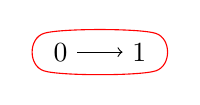
\begin{tikzpicture}[baseline={(0,-0.2)}]
        \node (A) at (0,0) {$0$};
        \node (B) at (1,0) {$1$};
        \draw [->] (A) -- (B);
        \draw [red] plot [smooth cycle] coordinates {(A.north west) (A.south west) (B.south east) (B.north east) };
     \end{tikzpicture}
     \right\}
     \xrightarrow{d^0}
     \left\{
     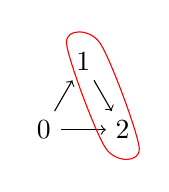
\begin{tikzpicture}[baseline={(0,0.3)}]
        \node (A) at (0,0.866) {$1$};
        \node (B) at (-0.5,0) {$0$};
        \node (C) at (0.5,0) {$2$};
        \draw [->] (A) -- (C);
        \draw [->] (B) -- (A);
        \draw [->] (B) -- (C);
        \draw [red] plot [smooth cycle] coordinates {(A.north west) (A.north east) (C.south east) (C.south west) };
    \end{tikzpicture}
     \right\}=[2]
     $
\end{tabular}
\]
We obtain for any simplicial set $ X $ a diagram
\[
\begin{tikzcd}
    X_n 
    \ar[r, " d_i" ]
    &
    X_{n-1}
    \\
    \Hom_{\SetD} ( \Delta^n , X )
    \ar[u, "\sim" {anchor=south, rotate=90} ]
    \ar[r, " ? \circ d^i_* " ]
    &
    \Hom_{\SetD} ( \Delta^{n-1} , X )
    \ar[u, "\sim" {anchor=south, rotate=90} ]
\end{tikzcd}
\]
and thus for any $ x \in X_n $ a diagram
\[
\begin{tikzcd}
    \Delta^n
    \ar[r , " x " ]
    &
    X
    \\
    \Delta^{n-1}
    \ar[ru]
    \ar[u,"d_*^i"]
    &
    .
\end{tikzcd}
\]
For $ n = 2 $ this looks explicitely as follows
\[
\begin{tikzcd}
    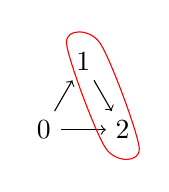
\begin{tikzpicture}
        \node (A) at (0,0.866) {$1$};
        \node (B) at (-0.5,0) {$0$};
        \node (C) at (0.5,0) {$2$};
        \draw [->] (A) -- (C);
        \draw [->] (B) -- (A);
        \draw [->] (B) -- (C);
        \draw [red] plot [smooth cycle] coordinates {(A.north west) (A.north east) (C.south east) (C.south west) };
    \end{tikzpicture}
    \ar[r , "x"]
    &
    X
    \\
    \tikz{
        \node (0) at (-0.5,0) {$0$};
        \node (1) at (0.5,0) {$1$};
        \draw [->] (0) to (1);
    \ar[ru]
    \ar[u]
    }
\end{tikzcd}     
\]
    
\begin{defi}
    The category $\Delta_{\txtbig}$ has as objects the finite non-empty total orders with order preserving maps between them
    \[
    \begin{tabular}{c}
         \begin{tikzcd}
             \Delta
             \arrow[r, hook, shift right]
             &
             \Delta_{\txtbig} 
             \arrow[l, shift right] \ni I = \{ i_0 < i_1 < \dotsc < i_n \}
         \end{tikzcd}      
    \end{tabular}
    \]
\end{defi}

This time we take a closer look at the diagrams that arise from the inclusions of partial orders.

\[
\begin{tabular}{cc}
     \begin{tikzcd}
         \{1\}
         \arrow[r, hook]
         &
         \{0 \to \circled{1}\}
     \end{tikzcd}
     \\
     \begin{tikzcd}
         \{0\}
         \arrow[r, hook]
         &
         \{\circled{0} \to 1\}
     \end{tikzcd}
     \\
     $
     \left\{
     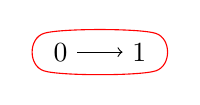
\begin{tikzpicture}[baseline={(0,-0.2)}]
        \node (A) at (0,0) {$0$};
        \node (B) at (1,0) {$1$};
        \draw [->] (A) -- (B);
        \draw [red] plot [smooth cycle] coordinates {(A.north west) (A.south west) (B.south east) (B.north east) };
     \end{tikzpicture}
     \right\}
     \xhookrightarrow{}
     \left\{
     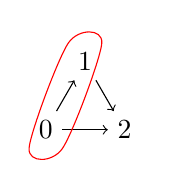
\begin{tikzpicture}[baseline={(0,0.3)}]
        \node (A) at (0,0.866) {$1$};
        \node (B) at (-0.5,0) {$0$};
        \node (C) at (0.5,0) {$2$};
        \draw [->] (A) -- (C);
        \draw [->] (B) -- (A);
        \draw [->] (B) -- (C);
        \draw [red] plot [smooth cycle] coordinates {(A.north west) (A.north east) (B.south east) (B.south west) };
    \end{tikzpicture}
     \right\}
     $
     \\
     $
     \left\{
     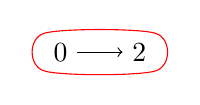
\begin{tikzpicture}[baseline={(0,-0.2)}]
        \node (A) at (0,0) {$0$};
        \node (B) at (1,0) {$2$};
        \draw [->] (A) -- (B);
        \draw [red] plot [smooth cycle] coordinates {(A.north west) (A.south west) (B.south east) (B.north east) };
     \end{tikzpicture}
     \right\}
     \xhookrightarrow{}
     \left\{
     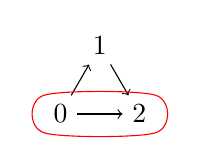
\begin{tikzpicture}[baseline={(0,0.3)}]
        \node (A) at (0,0.866) {$1$};
        \node (B) at (-0.5,0) {$0$};
        \node (C) at (0.5,0) {$2$};
        \draw [->] (A) -- (C);
        \draw [->] (B) -- (A);
        \draw [->] (B) -- (C);
        \draw [red] plot [smooth cycle] coordinates {(B.north west) (B.south west) (C.south east) (C.north east) };
    \end{tikzpicture}
     \right\}
     $
\end{tabular}
\]
These inclusions yield the following poorly organized faces of a square
\[
\begin{tikzcd}
    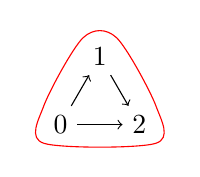
\begin{tikzpicture}
        \node (A) at (0,0.866) {$1$};
        \node (B) at (-0.5,0) {$0$};
        \node (C) at (0.5,0) {$2$};
        \draw [->] (A) -- (C);
        \draw [->] (B) -- (A);
        \draw [->] (B) -- (C);
        \draw [red] plot [smooth cycle] coordinates {(B.north west)  (A.north west) (A.north east) (C.north east) (C.south east) (B.south west) };
    \end{tikzpicture}
    &
    &
    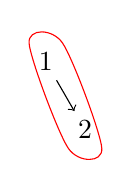
\begin{tikzpicture}
        \node (A) at (0,0.866) {$1$};
        \node (C) at (0.5,0) {$2$};
        \draw [->] (A) -- (C);
        \draw [red] plot [smooth cycle] coordinates {(A.north east)  (C.south east) (C.south west) (A.north west) };
    \end{tikzpicture}
    \ar[ll]
    \\
    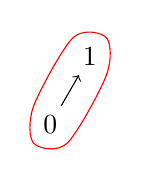
\begin{tikzpicture}
        \node (A) at (0,0.866) {$1$};
        \node (B) at (-0.5,0) {$0$};
        \draw [->] (B) -- (A);
        \draw [red] plot [smooth cycle] coordinates {(B.north west) (A.north west) (A.north east) (A.south east) (B.south east) (B.south west)};
    \end{tikzpicture}
    \ar[u]
    &
    \begin{tikzpicture}
        \node (A) at (0.0) {$1$};
        \draw [red] plot [smooth cycle] coordinates {(A.north west) (A.north east) (A.south east) (A.south west)};
    \end{tikzpicture}
    \ar[l]
    \ar[ru]
    \\
    &
    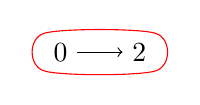
\begin{tikzpicture}[baseline={(0,-0.2)}]
        \node (A) at (0,0) {$0$};
        \node (B) at (1,0) {$2$};
        \draw [->] (A) -- (B);
        \draw [red] plot [smooth cycle] coordinates {(A.north west) (A.south west) (B.south east) (B.north east) };
     \end{tikzpicture}
     \ar[luu]
     &
     \begin{tikzpicture}
        \node (A) at (0.0) {$2$};
        \draw [red] plot [smooth cycle] coordinates {(A.north west) (A.north east) (A.south east) (A.south west)};
    \end{tikzpicture}
    \ar[l]
    \ar[uu]
    \\
    \begin{tikzpicture}
        \node (A) at (0.0) {$0$};
        \draw [red] plot [smooth cycle] coordinates {(A.north west) (A.north east) (A.south east) (A.south west)};
    \end{tikzpicture}
    \ar[uu]
    \ar[ru]
\end{tikzcd} 
\]
which looks applied to a simplicial set as follows
\[
\begin{tikzcd}
    X_2
    \ar[rr]
    \ar[rd]
    \ar[dd]
    &
    &
    X_{\{1 \to 2 \}}
    \ar[rd]
    \ar[dd]
    \\
    &
    X_{\{ 0 \to 2\}}
    \ar[dd]
    \ar[rr]
    &&
    X_{\{2\}}
    \\
    X_{\{0 \to 1 \}}
    \ar[rr]
    \ar[rd]
    &&
    X_{\{1\}}
    \\
    &
    X_{ \{ 0 \} }
\end{tikzcd}
\]
We furthermore have the co-degeneracy maps $ s^i \colon [ n + 1 ] \to [ n ] $ which are the unique order preserving surjective map, that take the value $ i $ twice.
This can be visualised as follows:
\[
\begin{tikzcd}
    0
    \ar[r]
    \ar[d]
    &
    1
    \ar[r]
    \ar[d]
    &
    \dots
    \ar[r]
    &
    i-1
    \ar[d]
    \ar[r]
    &
    i
    \ar[d]
    \ar[r]
    &
    i+1
    \ar[dl]
    \ar[r]
    &
    \dots
    \ar[r]
    &
    n+1
    \ar[dl]
    \\
    0
    \ar[r]
    &
    1
    \ar[r]
    &
    \dots
    \ar[r]
    &
    i-1
    \ar[r]
    &
    i
    \ar[r]
    &
    \dots
    \ar[r]
    &
    n
\end{tikzcd}
\]
and we obtain the following simplex diagram
\[
\begin{tikzcd}
    \Delta^{n+1}
    \ar[r]
    \ar[rd, dashed]
    &
    \Delta^n
    \ar[d, "x"]
    \\
    &
    X
\end{tikzcd}
\]

\begin{exmp}
    Let $ I \in \Set $, we can define the constant simplicial set associated to $ I $, where for all $ n \geq 0 $ we have $ I_n = I $, the faces and degeneracies are the identity functor.    
\end{exmp}

\begin{exmp}
    Let $\mathcal{C}$ be a small category. 
    We define $N(\mathcal{C}) \in \Set_{\Delta}$ as follows. 
    Let $N(\mathcal{C})_0 \coloneqq \Ob(\mathcal{C})$, $N(\mathcal{C})_1=\Mor(\mathcal{C})\colon$ set of morphisms in $\mathcal{C}$ with the face and boundary maps given as follows
    \[
    \begin{tikzcd}
        N ( \mathcal{ C } )_1 
        \ar[r, shift left=1.75ex, "d_0=target"]
        \ar[r, shift right=1.75ex, "d_1=source"']
        &
        N ( \mathcal{ C } )_0
        \ar[l, "s_1"]
    \end{tikzcd}
    \]
    where $ s_1(X) = X \xrightarrow{\id_X} X $ for an $ X \in \Ob ( \mathcal{ C } ) $. Now
    \[
    N ( \mathcal{ C } )_2 =
    \left\{
    \begin{tikzcd}
        &
        f_1
        \ar[rd, "f_{21}"]
        &
        \\
        f_0
        \ar[ru, "f_{10}"]
        \ar[rr, "f_{20}"]
        &&
        f_2
    \end{tikzcd}
    \mid f_{20} = f_{21} \circ f_{10}
    \right\}
    \]
    and we have degeneracies and codegeneracies
    \[
    \begin{tikzcd}
        N ( \mathcal{ C } )_2
        \ar[r, shift left= 2.75ex, "d_0"]
        \ar[r, "d_1" description]
        \ar[r, shift left= -2.75ex, "d_2"']
        &
        N ( \mathcal{ C } )_1
        \ar[l, shift left= - 1.25ex, "s_0"']
        \ar[l, shift left= 1.25ex,"s_1"]
    \end{tikzcd}.
    \]
    Now lastly 
    \[
    N ( \mathcal{ C } )_3 
    =
    \left\{
    \begin{tikzcd}
        & 
        f_1
        \ar[rd, "f_{21}"]
        \ar[dd, "f_{13}" pos=0.7]
        &
        \\
        f_0
        \ar[ru, "f_{10}"]
        \ar[rd, "f_{30}"]
        \ar[rr, dashed, "f_{20}" pos=0.3]
        &&
        f_2
        \ar[dl, "f_{23}"]
        \\
        &
        f_3
        &
    \end{tikzcd}
    \mid \forall i \leq j \leq k 
    f_{kj} \circ f_{ji} = f_{ki}
    \right\}.
    \]
    This gives a functor $ N ( \mathcal{ C } ) \colon \Delta^{\op} \to \Set $ where $ [ n ] \mapsto \Fun( [n] , \mathcal{ C } )$ and thus a simplicial set.
    Note that the nerve has a left adjoint given by the truncation functor.
\end{exmp}

\begin{exmp}
    Let $ X $ be a topological space we define $ \Sing ( X ) $ to be its associated singular simplicial set.
    \begin{itemize}
        \item 
         Let $\Sing ( X )_n \coloneqq \Hom_{\Top} ( \lvert \Delta^n \rvert , X ) $, where $ \lvert \Delta^n \rvert \coloneqq \{ v \in \mathbb{ R }_{\leq 0 }^{n+1}, \lvert \sum_{ i = 0 }^n v_i \rvert = 1 \}$.
        \item 
        For a morphism $ \sigma \colon [ m ] \to [ n ] $ we obtain a morphism $\sigma_* \colon \lvert \Delta^m \rvert \to \lvert \Delta^n \rvert $, where $ \sigma_*( v )_i= \sum_{ j \in \sigma^{-1} ( i ) } v_j$.
    \end{itemize}
    Note that $ \Sing $ has a left adjoint given by the geometric realisation functor.
\end{exmp}

\begin{thm}
    For all $X \in \Set_{\Delta}$ $\lvert X \rvert = \colim_{\substack{([n],x)\in \int_X^\Delta \\
    X\colon \Delta^n \dashv X} }\lvert \Delta^n\rvert$ is a CW complex.
\end{thm}

\begin{defi}
    An element $x$ of simplicial set $X$ is \underline{degenerate} if $x \in \im s_i$ for some $i$.
\end{defi}

\begin{rmk}
    Let $ N ( [ n ] ) = \Hom_{\Cat} ( [ ? ] , [ n ] ) \cong \Hom_{ \Delta } ( [ ? ] , [ n ] ) = \Delta^n $.
    Furthermore for $ \mathcal{ P } $ a poset, let $ N ( \mathcal{ P } )_n = \Hom_{Poset} ( [ n ] , \mathcal{ P } ) $.
    Take now a morphism $ [ n ] \coloneqq \{ 0 < 1 < 2 < \dotsc < n \} \xrightarrow{ \sigma } \mathcal{ P } $ and $ \sigma = ( \sigma_0 , \sigma_1 , \dotsc , \sigma_n ) \in \mathcal{ P }^{n+1} $ such that $ \sigma_0 \leq \sigma_1 \leq \dotsc \leq \sigma_n $, we call this a chain in the poset. 
    Let us now compute $ \Delta^2 = N ( [ 2 ] ) $, we denote the chain $\sigma = ( \sigma_0 , \sigma_1 , \dotsc , \sigma_n )$ by $\sigma_0  \sigma_1  \dotsc  \sigma_n$ in the following table.
    \[
    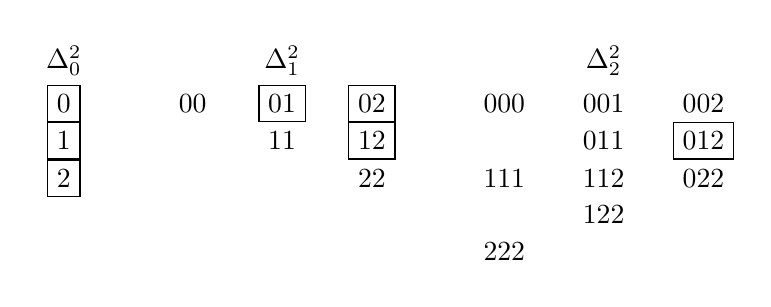
\begin{tikzpicture}
    \matrix [column sep=0.5cm]
    {
    \node{$\Delta_0^2$} ;& ;& ;& \node{$\Delta_1^2$} ;& ;& ;& ;& \node{$\Delta_2^2$} ;&
    \\
    \node[draw] {0}; & ;& \node{00}; & \node[draw]{01}; & \node[draw]{02}; & ;& \node {000}; & \node {001}; & \node {002};
    \\
    \node[draw] {1}; & ;& ;&\node{11};& \node[draw]{12}; & ;& ;& \node {011}; & \node[draw]{012};
    \\
    \node[draw] {2}; & ;& ;& ;& \node{22}; & ;& \node {111};& \node {112};& \node {022}; 
    \\
    ;&;&;&;&;&;&;& \node {122}; &;
    \\
    ;&;&;&;&;&;& \node {222} ;&;&;
    \\
    };
    \end{tikzpicture}
    \]
    The encircled chains correspond to non-degenerate simplices.
    
\end{rmk}

\begin{defi}
    Let $ X \in \SetD $ we write $ \dim X \leq k $ if $ \forall n > k $ we have that $ X_n = X_n^{degeneracies} $.
\end{defi}

We have a functor that goes from simplicial sets to simplicial groups and is similar to the free functor from set to abelian groups.
\[
\begin{tikzcd}
    X \in \SetD = \Fun ( \Delta^{\op}, \Set ) 
    \ar[d, "\mathbb{Z}"]
    \\
    \Ab_{\Delta} = ( \Fun ( \Delta^{ \op } , \Ab ) )
\end{tikzcd}
\]
We write $ ( \mathbb{ Z } X )_n = \mathbb{ Z } \langle X_n \rangle $.
Let now $ Y \in \Ab_{\Delta} $ be a simplicial abelian group, we associate to it a chain complex $ C ( Y ) \in \Ch_{\geq 0 } ( \Ab ) $, where $C ( Y )_n \coloneqq Y_n$ and the differential is given as 
\begin{align*}
    C ( Y )_n 
    &\to 
    C ( Y )_{ n -1 }
    \\
    x 
    &\mapsto
    \partial ( x ) = \sum_{i = 0}^n (-1)^i d_i ( x ).
\end{align*}

\begin{rmk}
    \begin{enumerate}
        \item 
        If we now take $ X \in \Top $ we can take $ \Sing ( X ) \in \SetD $ then $ \mathbb{ Z } \Sing ( X ) \in \Ab_{\Delta} $ and then $ C ( \mathbb{ Z } \Sing ( X ) ) \in \Ch_{\geq 0}$ with its $n$-th component being given by $ \mathbb{ Z } \langle \Hom_{ \Top } ( \lvert \Delta^n \rvert , X ) \rangle \in \Ab $.
        This complex is called the Moore complex and its associated homology groups give the integral singular homology $ H_* ( X ; \mathbb{ Z } ) $ of the space $ X $.
        Furthermore we can define the homology groups $ H_n( Y , A )$ of a simplical set $ Y $ with coefficients in an abelian group $ A $ to be the homology groups $ H_n ( \mathbb{ Z } Y \otimes A )$ of the chain complex $ \mathbb{ Z } Y \otimes A $.

        \item 
        Let $ \mathcal{ A } $ be an exact category. 
        Then $\mathcal{ A } $ has an associated category $ Q \mathcal{ A } $ with objects those of $ \mathcal{ A } $ and arrows given by equivalence classes of diagrams 
        \[
            \bullet \twoheadleftarrow \bullet \rightarrow \bullet
        \]
        where both arrows are parts of exact sequences of $ \mathcal{ A } $, and composition is represented by pullback. 
        Then $ K_{i-1} ( \mathcal{ A } ) \coloneqq \pi_i \lvert BQ\mathcal A \rvert $ defines the $ K $-groups of $ \mathcal{ A } $ for $  i \geq 1 $; in particular $ \pi_i \lvert B Q \proj ( R ) \rvert = K_{i-1} ( R )$, the $ i^{th}$ algebraic $K$-group of the ring $ R $, here $ \proj ( R ) $ denotes the category of finitely generated projectives over $ R $.
    \end{enumerate}
\end{rmk}

\begin{defi}
    The normalized Moore chain of $ Y $ is the chain complex with components $ \overline{C} ( Y )_n \coloneqq \bigcap_{ i = 1 }^n \ker d_i $ and differentials $ \partial_n = d^n_0 $.
\end{defi}

\begin{thm}(Dold-Kan Correspondences)
    Let $ \Delta \to \Ch_{ \geq 0 } $ be given by $ [n ] \mapsto \overline{C} ( \mathbb{ Z } ) \Delta^n $, then there exists an adjunction.
    \[
    \begin{tikzcd}
        \Bar{C}\colon \Ab_{\Delta}
        \ar[r, shift left]
        &
        \Ch_{ \geq 0 }( \Ab ) : DK 
        \ar[l , shift left, "\sim"]
    \end{tikzcd}
    \]
\end{thm}

\subsection{Exercises}

\begin{Exercise}
        Show that the functor $ \widehat{ \Delta }  \to \SetD $ which remembers only the face and degeneracy maps and is the identity on morphisms is an isomorphism of categories. 
        In particular,
         \begin{itemize}
             \item 
             show that the functor is well defined by showing that the co-face and co-degeneracy maps satisfy the cosimplicial identities.
             \begin{align*}
                 d^jd^i &= d^i d^{j-1} \quad \text{ if } i < j
                 \\
                 s^j s^i &= s^i s^{j+1} \quad \text{ if } i \leq j
             \end{align*}
             \qquad
             $
             s^j d^i=
             \begin{cases}
                 d^i s^{j-1} &\text{ if } i < j 
                 \\
                 \id &\text{ if } i \in \{ j , j + 1 \}
                 \\
                 d^{i-1} s^j &\text{ if } i > j = 1
             \end{cases}
             $
             Recall that the co-face maps $ d^i \coloneqq d_n^i $ and co-degeneracy maps $ s^i \coloneqq s_n^i $ are defined as follows for each $ n \in \mathbb{ N }_+ $ respective $ n \in \mathbb{ N }_0 $ and $ 0 \leq i \leq n $.  
             \begin{align*}
                 d^i = d_n^i \colon [ n - 1 ] &\to [ n ]
                 \\
                 k &\mapsto 
                 \begin{cases}
                     k & \text{ if } k < i 
                     \\
                     k+1 & \text{ if } i \leq k 
                 \end{cases}
             \end{align*}
             \quad
             \begin{align*}
                 s^i = s_n^i \colon [ n n 1 ] &\to [ n ]
                 \\
                 k &\mapsto 
                 \begin{cases}
                     k & \text{ if } k \leq i 
                     \\
                     k-1 & \text{ if } i < k 
                 \end{cases}
             \end{align*}
        
             \item  
             For the inverse, show that a morphism $ \sigma \colon [m] \to [n] $ in $ \Delta $ can be uniquely written as
            \[
                \sigma 
                =
                d_n^{i_s}
                \circ d_{ n - 1 }^{i_{s-1}} 
                \circ 
                \dotsm 
                \circ
                d_{ n - s + 1 }^{i_1}
                \circ
                s_{ m - t }^{j_1}
                \circ 
                \dotsm
                \circ
                s_{ m - 2 }^{ j_{t-1}}
                \circ 
                s_{ m - 1 }^{j_t}
            \]
            with $ 0 \leq i_1 < i_2 < \dotsm < i_s \leq n $ and $ 0 \leq j_1 < j_2 < \dotsm < j_t < m $ and $ n-s = m-t $.
        \end{itemize}
    \end{Exercise}
    
    \begin{Exercise}
        
    Fix $ n \in \mathbb{ N }_+ $.
    Define the simplicial subset $ \partial \Delta^n \subseteq \Delta^n $ by
    \[
        \partial \Delta^n ( [ m ] ) \coloneqq \{ \sigma \colon [ m ] \to [ n ] \text{ non-surjective } \}
    \]
    and similarly, define for $ 0 \leq k \leq n $ the simplicial subset $ \Lambda_k^n \subseteq \partial \Delta^n $ by
    \[
        \Lambda_k^n( [ m ] ) \coloneqq \{ \sigma  \in \partial \Delta^n ( [ m ] ) \mid \sigma ( [ m ] ) \neq [ n ] \setminus \{ k \} \}.
    \]
    \begin{enumerate}[label=(\alph*)]
        
        \item 
        Confirm that the above are indeed simplicial subsets.
    
        \item 
        Show one of the following 
        \begin{itemize}
        
            \item 
            $ \partial \Delta $ is the smallest simplicial subset of $ \Delta^n $ such that $ \{ d_n^i \mid 0 \leq i \leq n \} \subseteq \partial \Delta^n ( [ n - 1 ] ) $.
    
            \item 
            $\Lambda_k^n$ is the smallest simplicial subset of $ \Delta^n $ such that $ \{ d_n^i \mid 0 \leq i \leq n \wedge i \neq k \} \subseteq \Lambda^n_k ( [ n - 1 ] )$.
            
        \end{itemize}
    
    Recall that we may view $ \Delta $ as a category of posets, so that we may compute the nerve of ( subsets of ) $ [ n ] $ as partially ordered set.
    Moreover, we may associate to $ [ n ] $ the category $ \Sub_* ( [ n ] ) $ of non-empty proper full subcategories, i. e. $ [ n ] \notin \Sub_* ( [ n ] ) $, and morphisms given by inclusions.
    Similarly, we define for $ k \in [ n ] $ the full subcategory $ \Sub_*^k ( [ n ] ) \coloneqq \{ k \in E \in \Sub_* ( [ n ] ) \subseteq  \Sub_* ( [ n ] )$.
    
        \item 
        Show one of the following.
    
        \begin{enumerate}
            \item 
            \[
                \partial \Delta^n
                \cong 
                \bigcup_{ E \in \Sub_* ( [ n ] ) } N ( E ) \coloneqq 
                \colim_{ E \in \Sub_* ( [ n ] ) } N ( E ) 
            \]
    
            \item 
            \[
                \partial \Delta^n
                \cong
                \bigcup_{ E \in \Sub_* ( [ n ] ) } N ( E ) \coloneqq 
                \colim_{ E \in \Sub_* ( [ n ] ) } N ( E ) 
            \]
        \end{enumerate}
    
        \item 
        Justify the notation $ \bigcup $.
        
    \end{enumerate}
\end{Exercise}

\begin{Exercise}
    Let $ \Delta_{ \leq n } $ be the full subcategory of $ \Delta $ of the elements $ [ 0 ] , [ 1 ] , \dotsc , [ n ] $.
    The inclusion $ \iota_n \colon \Delta_ { \leq n } \to \Delta $ induces a truncation functor $ \tr_n \coloneqq ( \iota_n )^* \colon \Set_{ \Delta } \to \widehat{ \Delta_ { \leq n } } $.

    \begin{enumerate}[label=(\alph*)]
        
        \item 
        Show that $ \tr_n $ admits both a left and a right adjoint, $ \sk_n \dashv \tr_n \dashv \cosk_n $, which are both fully faithful.
    
        \item 
        Deduce that we have an adjunction $ \bold{sk_n} \coloneqq \sk_n \circ \tru_n \dashv \cosk_n \circ\tru_n \eqqcolon \bold{ cosk_n } $ of endofunctors of $ \SetD $.
        
    \end{enumerate}
    
    The essential image of $ \sk_n $ are called the $ n $-skeletal simplicies while the essential image of $ \bold { cosk_n } $ are the $ n $-coskeletal simplices.
    
    \begin{enumerate}[label=(\alph*), resume]
        \item 
        Show that a simplicial set $ X $ is $ n $-skeletal if and only if 
        
        $ \tru_n \colon \Hom_{ \SetD } ( X , - ) \to \Hom_{ \widehat{ \Delta{ \leq n }}} ( \tru_n X , \tru_n ( - ) ) $ is an isomorphism of functors.
    
        \item 
        Show that a simplicial set $ Y $ is $ n $-coskeletal if and only if
        
        $ \tru_n \colon \Hom_{ \Set_\Delta } ( - , Y ) \to \Hom_{ \widehat{ \Delta_{ \leq n }} } ( \tru_n ( - ) , \tru_n Y ) $ is an isomorphism of functors.
    \end{enumerate}
\end{Exercise}

\begin{Exercise}
    \begin{enumerate}[label=(\alph*)]
         \item 
         Show that a map $ F \colon X  \to N ( \mathcal{ C } ) $ to the nerve of a category $ \mathcal{ C } $, is completely determined by a map $ u \colon X_1 \to \Mor ( \mathcal{ C } ) $ such that 
         \begin{enumerate}
             \item 
             for all $ x \in X_0 $ we have that $ u ( s_0 ( x ) ) $ is an identity and 
    
             \item 
             for any $2$-simplex $ \sigma \in X_2 $ we have that $ u ( d_1 ( \sigma ) ) = u ( d_0 ( \sigma ) ) \circ u ( d_2 ( \sigma ) )$.
         \end{enumerate}
    
         \item 
         Deduce that the nerve of a category is 2-coskeletal.
    
         \item 
         Conclude that the nerve $ N \colon \Cat \to \SetD $ is fully faithful.
    \end{enumerate}
\end{Exercise}

\begin{Exercise}
    Consider the functor $ \Op \colon \Delta \to \Delta $ which is the identity on objects and for $ \sigma : [ n ] \to [ m ] $
    \[
        \Op ( \sigma ) ( i ) 
        \coloneqq
        m - \sigma ( n - i )
    \]
    Let $ ( - )^{ \op } \coloneqq \Op^* \colon \SetD \to \SetD $ be the corresponding involution of the category of simplicial sets.
    
    \begin{enumerate}[label=(\alph*)]
        \item 
        Show that $ \Op $ is a well defined involution.
    
        \item 
        For a simplicial set $ X $, describe the face and degeneracy maps of $ X ^{ \op } $.
    
        \item 
        Show that for a category $ \mathcal{ C } $ we have an isomorphism $ N ( \mathcal{ C }^{\op} ) \cong N ( \mathcal{ C } )^{\op} $.
    
        \item   
        Show that for a topological space there is an isomorphism $ \Sing ( X ) \cong \Sing ( X )^{ \op } $ for the singular complex of $ X $.
    \end{enumerate}
\end{Exercise}
Lecture 12.11

\section{Connected components \& the fundamental groupoid I}

Consider the following functors
\[
\begin{tikzcd}
    \Set 
    \arrow[r, hook, bend left, "\iota" pos= 0.55,""{name=A, above}]
    &
    \Gpd
    \arrow[l, bend left ,"\pi_0" pos=0.4,""{name=B, above}]
    \ar[from=A, to=B, symbol=\dashv]
    \ar[r, bend left, "j",""{name=E, above}]
    &
    \Cat
    \ar[l, bend left, "L" pos=0.6,""{name=F, below}]
    \ar[from=E, to=F , symbol=\dashv]
    \ar[r, hook, bend left, "N",""{name=C, above}]   
    &
    \Set_{\Delta}
    \ar[l, bend left, "\tau" pos= 0.45,""{name=D, below}]
    \ar[from=C, to=D , symbol=\dashv] 
\end{tikzcd}
\]

These functors admit left adjoints:
Given $G \in \Gpd$ we let $\pi_0(G) \in \Set$ be its set of isoclasses.

\begin{prop}
    The canonical functor  $G \to \iota(\pi_0(G))$, $G \in \Gpd$ are the components of the unit of an adjunction 
    \[
    \begin{tikzcd}
        \pi_0\colon \Gpd 
        \ar[r,shift left]
        &
        \Set : \iota
        \ar[l,shift left, "\adj" ]
    \end{tikzcd}
    \]
\end{prop}

\begin{proof}
    Let $J \in \Set$ and let $F$ be a functor $F \colon G \to \iota(J)$. We observe that $\forall f \colon X \to Y$ in $G$ we have $F(f) = \id_{F(x)}=\id_{F(y)}$
    in other words, $F$ is a constant on isomorphism-classes in $G$, hence $F$ factors uniquely through $G \xrightarrow{\eta_g} \iota(\pi_0(G))$.
    \[
    \begin{tikzcd}
        G 
        \ar[r,"\eta_g"]
        \ar[rd, "\forall F"']
        &
        \iota(\pi_0(G))
        \ar[d,"\iota(\Bar{F})"]
        \\
        &
        \iota(J)
    \end{tikzcd}
    \]
    This gives an isomorphism $\Hom_{\Set}(\pi_0(G),-) \cong \Hom_{\Gpd}(G,\iota(-))$, which means we have an adjunction $\pi_0 \dashv \iota$ with unit $\eta$.
\end{proof}

For $\mathcal{C} \in \Cat$ we define $L\mathcal{C} \in \Gpd$ as follows:
Consider the quiver with vertices $\Ob(\mathcal{C})$ and arrows $\Mor(\mathcal{C}) \amalg \{ f^{-} \mid f \in \Mor(\mathcal{C}) \}$.
For $f \in \Mor(\mathcal{C})$
\begin{center}
\begin{tabular}{cc}
    $s(f)=$ domain $f$ & $X \xrightarrow{f} Y$  
    \\
    $t(f)=$ codomain of $f$ &
    \\
    $s(f^{-})=$ codomain of $f$ & $X \xleftarrow{f^{-}}Y$
    \\
    $t(f^{-})=$ domain of $f$
\end{tabular}
\end{center}

Consider the quotient of the path category of the above quiver by the relation generated by 
\begin{itemize}
    \item 
    $\forall X \in \Mor(\mathcal{C}), \id_X \sim e_X\colon $ lazy path at $X$
    \item 
    $\forall f,g \in \Mor(\mathcal{C})$ composable $\cdot \xrightarrow{f} \cdot \xrightarrow{g} \cdot \sim \cdot \xrightarrow{g \circ f} \cdot$
    \item 
    $\forall f \in \Mor(\mathcal{C})$
    \begin{align*}
        \cdot \xrightarrow{f} \cdot \xrightarrow{f^-} \cdot \sim \id
        \\
        \cdot \xrightarrow{f^-} \cdot \xrightarrow{f} \cdot \sim \id
    \end{align*}
    that is $[f^-]=[f]^{-1}$
\end{itemize}

\begin{thm}
    The canonical functors $\gamma = \gamma_{\mathcal{C}}\colon \mathcal{C} \to L \mathcal{C}$, $\mathcal{C} \in \Cat$, form the components of the unit of an adjunction
    \[
    \begin{tikzcd}
        L\colon \Cat
        \ar[r]
        &
        \Gpd:j
    \end{tikzcd}
    \]
\end{thm}

\begin{proof}
    A functor $F \colon \mathcal{C} \to j(G)$, $G \in \Gpd$ nessecarily inverts all maps in $\mathcal{C}$ hence the functor $\Bar{F}(x) \coloneqq F(x)\colon L\mathcal{C} \to j(G)$ $F(f) \coloneqq F([f])$ $\Bar{([f^-])\coloneqq F(f)^{-1}}$ is well defined and is the unique functor such that 
    \[
    \begin{tikzcd}
        \mathcal{C} 
        \ar[r, "\gamma_{\mathcal{C}}"]
        \ar[dr, "F"']
        &
        j(L\mathcal{C})
        \ar[d, "j(\Bar{F})"]
        \\
        &
        j(G)
    \end{tikzcd}
    \]
    commutes, giving $L \dashv j$ with unit $\eta$.
\end{proof}

    Consider now for $X \in \Set_{\Delta}$, the quiver with vertices $X_0$ and arrows $X_1$ with $d_1=s\colon, X_1 \to X_0$ and $d_0= t\colon X_1 \to X_0 $. We have that $\tau(X)$ is the quotient of the path category of this quiver modulo the relation 
    \[
    \begin{tikzcd}
        &
        {}
        \ar[rd, "f_{21}"]
        &
        \\
        {}
        \ar[ru, "f_{10}"]
        \ar[rr, "f_{20}"']
        &
        &
        {}
    \end{tikzcd}
    \in X_2
    \implies 
    [f_{20}]=[f_{21}] \circ [f_{10}].
    \]   
    

\begin{prop}
    The canonical maps $\eta_X\colon X \to N(\tau X)$ ,  $X \in \Set_{\Delta}$ form the components of the unit of an adjunction 
    \[
    \begin{tikzcd}
        \tau\colon \Set_{\Delta}
        \arrow[r, shift left]
        &
        \Cat\colon N
        \arrow[l, shift left, "\adj"]
    \end{tikzcd}
    \]
\end{prop}

\begin{defi}
    We also have the composite adjunction
    \[
    \begin{tikzcd}
        \Set 
        \arrow[r, hook, bend left, "\iota" pos= 0.55,""{name=A, above}]
        \ar[rrr, bend right=50, ""]
        &
        \Gpd
        \arrow[l, bend left ,"\pi_0" pos=0.4,""{name=B, above}]
        \arrow[from=A, to=B, symbol=\dashv]
        \arrow[r, bend left, "j",""{name=E, above}]
        &
        \Cat
        \arrow[l, bend left, "L" pos=0.6,""{name=F, below}]
        \arrow[from=E, to=F , symbol=\dashv]
        \arrow[r, hook, bend left, "N",""{name=C, above}]   
        &
        \Set_{\Delta}
        \arrow[l, bend left, "\tau" pos= 0.45,""{name=D, below}]
        \ar[lll, bend right=50, "\mathbb{\pi}_0"']
        \arrow[from=C, to=D , symbol=\dashv] 
    \end{tikzcd}    
    \]
    \begin{tikzcd}
        \pi_0\coloneqq \pi_0 \circ L \circ \tau \colon \Set_{\Delta}
        \arrow[r, shift left]
        &
        \Cat\colon N \circ j \circ \iota
        \arrow[l, shift left, "\adj"]
    \end{tikzcd}
\end{defi}

\begin{defi}
    For $ X \in \Set_{\Delta}$ we call $\pi_0(X)\in \Set$ is a \underline{connected component}.
    For $ I \in \Set$ we have that
    \[
    N(j(\iota(I)))_n=N(\iota(I))_n=\Hom_{\Cat}([n], \iota(I)) \cong I
    \]
    which means that 
    \[
    N \circ j \circ \iota = \const_{\Delta}
    \]
    By uniqueness of adjoints we obtain that $\pi_0 \cong \colim_{\Delta}$ is adjoint to $\const_{\Delta} \cong N \circ j \circ \iota$ where $\pi_0(X)\cong X_0 / \sim$ and $X \sim Y$ if and only if there exists a zigzag of edges in $X$.
    Consider now the composite adjunction
\end{defi}
    \[
    \begin{tikzcd}
        \Gpd
        \arrow[r, bend left, "j",""{name=A, above}]
        \arrow[rr, bend left=50, "\pi_1"]
        &
        \Cat
        \arrow[l, bend left ,"L" pos=0.45,""{name=B, above}]
        \arrow[from=A, to=B, symbol=\dashv]
        \arrow[r, bend left, "N",""{name=C, above}]
        &
        \Set_{\Delta}       
        \arrow[l, bend left ,"\tau" pos=0.45,""{name=D, above}]
        \arrow[from=C, to=D, symbol=\dashv]
        \arrow[ll, bend left=55, "N"]
    \end{tikzcd}
    \]
    Where 
    \begin{tikzcd}
        \pi_1\coloneqq L \circ \tau \colon \Set_{\Delta}
        \arrow[r, shift left, "\Gpd"]
        &
        \Gpd \colon N \circ j = N_{\mid \Gpd}=N
        \arrow[l, shift left, "\adj"]
    \end{tikzcd}

\begin{defi}
    For $X \in \Set_{\Delta}$ we call $\pi_1(X)\in \Gpd$ its \underline{fundamental groupoid}.
    For $x \in X_0$ we define $\pi_1(X,x) \in \Grp$ as 
    \[
    s_0(x)=[1_x] \in \Hom_{\pi_1(X)}(x,x)
    \]
    Let $f \colon X \to Y$ in $\Set_{\Delta}$ be a morphism then we get a functor $\pi_1(X) \to \pi_1(Y)$ given as 
    \[
    \begin{tikzcd}
        \pi_1(f)\colon \pi_1(X,x)=\Hom_{\pi_1(X)}(x,x)
        \arrow[r]
        &
        \Hom_{\pi_1(Y)}(f_0(x),f_0(x))=\pi_1(Y,f_0(x))
    \end{tikzcd}
    \]
\end{defi}

Lecture:14.11 

\subsection{connected component}

We have the adjunction $\pi_0 \colon \SetD$
\[
\begin{tikzcd}
    \pi_0(X)\cong \coeq(X_1
    \arrow[r, shift left, "d_1"]
    \arrow[r, shift right, "d_0"']
    &
    X_0)
\end{tikzcd}
\]
For $X \in \Set_{\Delta}$ we have the unit morphism $\eta_X \colon X \to \pi_0(X)$.
When $\eta_X$ is an isomorphism we say that $X$ is \underline{discrete}.



We want to show that $X \in  \Set_{\Delta}$ decomposes as the disjoint union of the connected simplicial subsets, called its \underline{connected components}.

\begin{construction}
    For $C \in  \pi_0(X)=X_0/\sim$ ( in particular $C \subseteq X_0$) let $X(C)_n \coloneqq \{ \sigma  \in X_n \mid \forall \Delta \xrightarrow{f}\Delta^n \xrightarrow{\sigma}X , \sigma \circ f\in C\}$.
    Notice that $X(C) \subseteq X$ is a simplicial subset since for $\sigma  \in X(C)_n$ and $\tau \colon \Delta^m \to \Delta^n$ we have that 
    \[
    \begin{tikzcd}
        \Delta^m
        \arrow[r,"\tau"]
        &
        \Delta^n
        \arrow[r,"\sigma"]
        &
        X
        \\
        \Delta^0
        \arrow[u,"v"]
        \arrow[ru]
    \end{tikzcd}    
    \]
\end{construction}

Moreover, $X(C) \subseteq X$ is a summand in the sense that $X \cong X(C) \amalg (X \setminus X(C))$ for $X_n \setminus X(C)_n$ also defines a simplicial subset.
\[
X_n\setminus X(C)_n =\{ \sigma  \in X_n \mid \forall \Delta \xrightarrow{f}\Delta^n \xrightarrow{\sigma}X,\sigma\circ f \notin C\}
\]

\begin{prop}
    The canonical map 
    \[
    \begin{tikzcd}
        \amalg_{C \in \pi_0(X)}X(C)
        \arrow[r, hook]
        &
        X
        \\
        X(C)
        \arrow[u, hook]
        \arrow[ru, "\iota_C"]
    \end{tikzcd}
    \]
    is an isomorphism of simplicial sets.
\end{prop}

\begin{rmk}
    Notice that
    $\pi_0(X(C))=\{C\}$ as well as 
    $\amalg_{C \in \pi_0(X)}\pi_0(X(C))
    =\pi_0(\amalg_{C \in \pi_0(X)}X(C)) 
    \isomorphism 
    \pi_0(X)$
\end{rmk}

\begin{prop}
    For any simplicial set $X \in \Set_{\Delta}$, that is not equal to the empty set, the following are equivalent 
    \begin{enumerate}
        \item 
        $\pi_0(X)=\{*\}$
        \item 
        if $X \cong Y \amalg Z$ then $Y = \emptyset$ or $Z = \emptyset$
    \end{enumerate}
    When this is the case we call $X$ \underline{connected}.
\end{prop}

\begin{proof}
    \begin{enumerate}
        \item 
        $''1)\implies2)''$
        We argue by contrapositive. 
        Let
        \[
        X \cong Y \amalg Z
        \] 
        such that neither $Y$ nor $Z$ are the empty simplicial set.
        Then we have that 
        \[
        \pi_0(X) \cong \pi_0(Y) \amalg \pi_0(Z) \neq \{ *\}
        \]
        \item 
        $''1)\implies2)''$
        We argue again by contrapositive. 
        \[
        \amalg_{C \in \pi_0(X)} X(C) \isomorphism X
        \]
        where at least two of the summands on the left are nonempty.
    \end{enumerate}
\end{proof}

\begin{prop}
    Let $\emptyset \neq X \in \Set_{\Delta}$ and $S\subseteq X$ a connected component, that is $\pi_0(S)=\{*\}$ and $X=S \amalg (X \setminus S)$.
    Then $\exists!C \in \pi_0(X)$ such that $S=X(C)$.
\end{prop}

\begin{prop}
    Let $X,Y$ be connected simplicial sets then $X  \times Y$ is connected. 
\end{prop}

\begin{proof}
    Let $(x,y),(x',y') \in (X\times Y)_0=X_0 \times Y_0$ and $X \xleftarrow{f}X''\xrightarrow{g}X'$ with $f,g \in X_1$ as well as $y \xrightarrow{h} y'$ with $h \in Y_1$.
    \[
    \begin{tikzcd}
        (x,y)
        \arrow[d,"{( 1_x , h )}"']
        &
        (x',y')
        \\
        (x,y')
        &
        (x'',y)
        \arrow[l, "{(f,1_{y'})}"]
        \arrow[u, "{(g,1_{y'})}"']
    \end{tikzcd}
    \]
    \begin{Warning}
        The collection of simplicial sets is not closed under infinite products.
        Take the nerve of the natural numbers $ N ( \mathbb{ N } ) $ as well ordered set and let $ X $ be the associated simplicial set, then $ S = \prod_{ n \in \mathbb{ Z }_{ \geq 0 } } X $ is not connected, since the element $ i = ( 0 , 0 , 0 ,\dotsc ) $ and $ j = ( 0 , 1 , 2 , 3 , \dotsc ) $ have no edge between one another, since edges in the product are finite compositions of tuples of edges in the components.
    \end{Warning}
\end{proof}

\begin{comment}
    
\section{boundaries and horns}

Let $X \in \Set_{\Delta}$ and $f,g \in X_1$ such that $d_0f=d_1g$, that is we have the following 
\[
d_1f\xrightarrow{f}d_0f=d_1g\xrightarrow{g}d_0g
\]
We would like to have a composite of $f$ and $g$, that is a commutative diagramm
\[
\begin{tikzcd}
    &
    a
    \arrow[rd, "g"]
    &
    \\
    b
    \arrow[ru, "f"]
    \arrow[rr, "n"']
    &
    &
    c
\end{tikzcd}
\in X_2
\]
We introduce the 2-horn at position 1 $\Lambda_1^2 \subseteq \Delta^2$ as the simplicial subset generated by $0 \xrightarrow{01}1$ and $1 \xrightarrow{12}2$, that is 
\[
\begin{tikzcd}
    &
    1
    \arrow[dr]
    &
    \\
    0
    \arrow[ur]
    &&
    2
\end{tikzcd}
=
\Lambda_1^2 
\xrightarrow{(f,g)}
X
\]
with $f,g \in X_1$ and $d_0f=d_1g$

\[
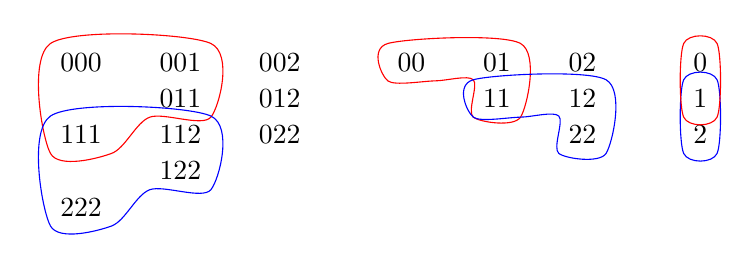
\begin{tikzpicture}
    \matrix[column sep = 0.5cm]
    {
    \node(000) {000};& \node(001) {001};& \node{002};&;& \node(00){00};& \node(01){01};& \node{02};&;& \node(0){0};\\
    &\node(011){011};& \node{012};&;&;& \node(11){11};& \node(12){12};&;& \node(1){1};\\
    \node(111){111};& \node(112){112};& \node{022};&;&;&;& \node(22){22};&;&\node(2){2};\\
    &\node(122){122};\\
    \node(222){222};\\
    };
    \draw [blue] plot [smooth cycle] coordinates { (1.north west) (1.north east) (2.south east) (2.south west)};
    \draw [red] plot [smooth cycle] coordinates { (0.north west) (0.north east) (1.south east) (1.south west)};
    \draw [red] plot [smooth cycle] coordinates { (00.north west) (01.north east) (11.south east) (11.south west) (11.north west) (00.south east) (00.south west)};
    \draw [blue] plot [smooth cycle] coordinates { (11.north west) (12.north east) (22.south east) (22.south west) (22.north west) (11.south east) (11.south west)};
    \draw [red] plot [smooth cycle] coordinates { (000.north west) (001.north east) (011.south east) (011.south west) (111.south east) (111.south west) };
    \draw [blue] plot [smooth cycle] coordinates { (111.north west) (112.north east) (122.south east) (122.south west) (222.south east) (222.south west) };
\end{tikzpicture}
\]

\[
\text{pushout:}
\begin{tikzcd}
    \Delta^0=\Delta^{\{1\}}
    \arrow[r,hook]
    \arrow[d,hook]
    &
    \Delta^{\{0,1\}}
    \arrow[d,"01"]
    \arrow[rdd,bend left]
    &
    &
    \\
    \Delta^{\{1,2\}}
    \arrow[rrd, bend right]
    \arrow[r, "12"]
    &
    \Lambda^2_1
    \arrow[rd,dashed,"\exists!"]
    &
    &
    \\
    &
    &
    X
\end{tikzcd}
\]

\todo{fill in the missing}
\end{comment}

\subsection{Exercises}

\begin{Exercise}
    Recall that we defined the connected component functor $ \pi_0 : \SetD \to \Set $ as 
    \[
        \pi_0 ( X ) \coloneqq \colim_{ \Delta } X 
    \]
    which yields a left adjoint to the constant diagram functor $ \const : \Set \to \SetD $.
    
    \begin{enumerate}[label=(\alph*)]
        
        \item 
        Show that $ \pi_0 ( \Delta^n ) $ is a one point set for any $ n \in \mathbb{ N } $.
    
        \item 
        Recall from Exercise 6.2 the boundaries $ \partial \Delta^n $ and horns $ \Lambda_k^n $ of $ \Delta^n $.
        Compute $ \pi_0 ( \partial \Delta^n ) $ and $ \pi_0 ( \Lambda_k^n ) $. 
    \end{enumerate}
    
    By definition the connected components of a small category $ \mathcal{ C }$ are defined as the coequalizer 
    \[
        \begin{tikzcd}
        \Mor ( \mathcal{ C } ) 
        \ar[r, shift left, "\text{target}"]
        \ar[r, shift right, "\text{source}"']
        &
        \Ob( \mathcal{ C } )
        \end{tikzcd}
    \]
    
    \begin{enumerate}[label=(\alph*), resume]
       
        \item 
        Show that for any simplicial set $ X $, the connected components $ \pi_0 ( X ) $ of $ X $ agree with the connected components of the category of elements $ \int^{ \Delta } X $.
    
        \item 
        Show that the connected components of a category $ \mathcal{ C } $ agree with the connected components of its nerve $ \pi_0 ( N ( \mathcal{ C } ) )$.
        
    \end{enumerate}
\end{Exercise}

\begin{Exercise}
    For a simplicial set $ X $, let $\bold{ Sk_n } ( X ) $ be the smallest simplicial subset of $ X $ such that $ ( \bold{ Sk_n } ( X ) )_m = X_m $ for $ m \leq n $.
    
    \begin{enumerate}
        \item 
        Show that there is a natural isomorphism $ \bold { Sk_n } ( X ) \cong \bold { sk_n } ( X ) $, i.e. $ \bold{ Sk_n } $ describes the $n$-skeleton functor from Exercise 6.2.
    \end{enumerate}
    
    Consider for any simplicial set $ X $ the canonical functor $ \bold{ sk }_X \colon \mathbb{ N }_0 \to \SetD $ with $ \bold{ sk }_X ( n ) \coloneqq \bold{ sk }_n ( X ) $ and morphisms induced by the inclusion $ \bold{ sk }_n ( X ) \subseteq X $.
    We call the image of $ \bold{ sk }_X $ the skeletal filtration of $ X $. 
    For convenience, we set $ \bold{ sk }_{-1} ( X ) $ to the empty presheaf.
    
    \begin{enumerate}[label=(\alph*), resume]
        \item 
        Argue that the morphisms in the skeletal filtration of $ X $ are monomorphisms and show that $ X \cong \colim_{ \mathbb{ N } } \bold{ sk }_X$.
    
        \item 
        Recall that $ \sigma \in X_n $ can be viewed as a morphism $ \sigma : \Delta^n \to X $.
        Observe that $ \sigma $ factors through $ \bold{ sk }_n ( X ) $ and that the precomposition of $ \sigma $ with the inclusion $ \partial \Delta^n \subseteq \Delta $ factors through $ \bold{ sk }_{n-1} ( X ) $.
        Show that these maps assemble into a pushout diagram.
        \[
        \begin{tikzcd}
            \coprod_{ \sigma \in X_n^{nd}} \partial \Delta^n
            \rar
            \dar
            &
            \coprod_{ \sigma \in X_n^{nd}} \Delta^n
            \dar
            \\
            \bold{sk_{n-1}}(X)
            \rar
            &
            \bold{sk_n}(X)
        \end{tikzcd}
    	\]
        Here $X_n^{nd} \coloneqq X_n \setminus ( \bold{ sk_{n-1} ( X ) })_n$ 
        denotes the set of non-degenerate $n$-simplicies in $ X$
    
        \item   
        Show that the geometric realisation of a simplicial set is a CW complex.
    \end{enumerate}
\end{Exercise}





%done

\section{Kan complexes}

lecture 19.11

For references for this section see \cite[Section I.3]{GoerSimp1999} \& \cite[Section 1.2.5]{kerodon}.

The aim of this chapter is to introduce a calss of simplicaial sets that behave simultaneously as nerves of groupoids and singular sets of spaces.

\begin{defi}
    Let $n \geq 1$ and $ 0 \leq k \leq n$.
    The $k$-th horn $\Lambda_k^n \subseteq \Delta^n$ is the simplicial subset generated by $\{ d^i \colon [n-1] \to [n] \mid 0 \leq i \leq n ; i \neq n \} = \Delta ( n-1,n) = (\Delta^n)_{n-1}$ , or equivalently $\Lambda_k^n = \colim_{\emptyset \neq k \in I \subsetneq [n]}\Delta^I$ where $\Delta^I \cong \Delta^{\lvert I \rvert -1}$.
\end{defi}

\begin{rmk}
    We will sometimes refer to $\Lambda_k^n$ as the $n$-horn at position $k$.     
\end{rmk}

\begin{exmp}
    Let us give a list for the horns up to dimension 3
    \begin{itemize}
        \item 
        For $ n = 1 $ we have the two horns $\Lambda_0^1 =0 $ and $\Lambda_1^1=1$.
        \item 
        For $ n = 2 $ we have the following 3 horns, given here with their embedding into the standard 2-simplex
        \[
        \Lambda_0^2 \colon 
        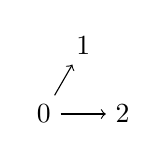
\begin{tikzpicture}[baseline={(0,0.3)}]
            \node (A) at (0,0.866) {$1$};
            \node (B) at (-0.5,0) {$0$};
            \node (C) at (0.5,0) {$2$};
            \draw [->] (B) -- (A);
            \draw [->] (B) -- (C);
        \end{tikzpicture}
        \hookrightarrow
        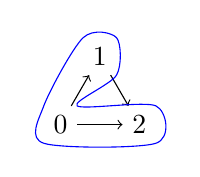
\begin{tikzpicture}[baseline={(0,0.3)}]
            \node (A) at (0,0.866) {$1$};
            \node (B) at (-0.5,0) {$0$};
            \node (C) at (0.5,0) {$2$};
            \draw [->] (A) -- (C);
            \draw [->] (B) -- (A);
            \draw [->] (B) -- (C);
            \draw [blue] plot [smooth cycle] coordinates {(A.north west)     (A.north east) (A.south east) (B.north east) (C.north east) (C.south east) (B.south west) (B.north west) };
        \end{tikzpicture}
        \]
        \[
        \Lambda_1^2 \colon 
        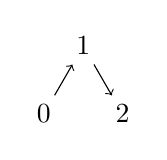
\begin{tikzpicture}[baseline={(0,0.3)}]
            \node (A) at (0,0.866) {$1$};
            \node (B) at (-0.5,0) {$0$};
            \node (C) at (0.5,0) {$2$};
            \draw [->] (B) -- (A);
            \draw [->] (A) -- (C);
        \end{tikzpicture}
        \hookrightarrow
        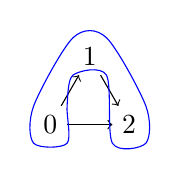
\begin{tikzpicture}[baseline={(0,0.3)}]
            \node (A) at (0,0.866) {$1$};
            \node (B) at (-0.5,0) {$0$};
            \node (C) at (0.5,0) {$2$};
            \draw [->] (A) -- (C);
            \draw [->] (B) -- (A);
            \draw [->] (B) -- (C);
            \draw [blue] plot [smooth cycle] coordinates {(A.north west) 
            (A.north east) (C.north east) (C.south east) (C.south west) (A.south east) (A.south west) (B.north east) (B.south east) (B.south west) (B.north west) };
        \end{tikzpicture}
        \]
        \[
        \Lambda_2^2 \colon 
        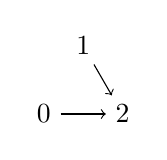
\begin{tikzpicture}[baseline={(0,0.3)}]
            \node (A) at (0,0.866) {$1$};
            \node (B) at (-0.5,0) {$0$};
            \node (C) at (0.5,0) {$2$};
            \draw [->] (A) -- (C);
            \draw [->] (B) -- (C);
        \end{tikzpicture}
        \hookrightarrow
        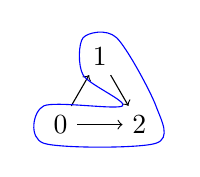
\begin{tikzpicture}[baseline={(0,0.3)}]
            \node (A) at (0,0.866) {$1$};
            \node (B) at (-0.5,0) {$0$};
            \node (C) at (0.5,0) {$2$};
            \draw [->] (A) -- (C);
            \draw [->] (B) -- (A);
            \draw [->] (B) -- (C);
            \draw [blue] plot [smooth cycle] coordinates {(A.south west) (A.north west) (A.north east) (C.north east) (C.south east) (B.south west) (B.north west) (C.north west) };
        \end{tikzpicture}
        \]
    \end{itemize}
\end{exmp}

\begin{rmk}
    The horn $\Lambda_k^n \subseteq \Delta^n$ enjoys the following universal property:
    For $X \in \SetD$ the map 
    \[
    \begin{tikzcd}
        \Hom_{\SetD}(\Lambda_k^n,X)
        \arrow[r, hook]
        &
        \prod_{\substack{0\leq i \leq \\ i \neq k}}
        \Hom_{\SetD}(\Delta^{n-1},X)
        \\
        \sigma 
        \arrow[r, mapsto]
        &
        (\sigma \circ d^i)_{\substack{0 \leq i \leq n \\ i \neq k}}
    \end{tikzcd}
    \]
    is injective, with image the subset of tuples $(\sigma_0,\sigma_1,\dotsc,\sigma_{k-1},\cdot, \sigma_{k+1}, \dotsc, \sigma_n) \in (X_{n-1})^n$ such that for all $ 0 \leq i < j \leq n$, $i \neq k$ $d_(\sigma_j)=d_{j-1}(\sigma_i)$ with $I = [n] \setminus \{i\}$ and $J=[n]\setminus \{j\}$ the following diagrams commute
    \[
    \begin{tikzcd}
    	& {\Delta^{I \cap J}} \\
    	{\Delta^I} && {\Delta^J} \\
    	& {\Lambda_k^n}
    	\arrow[hook', from=1-2, to=2-1]
    	\arrow[hook, from=1-2, to=2-3]
    	\arrow[from=2-1, to=3-2]
    	\arrow[from=2-3, to=3-2]
    \end{tikzcd}
    \qquad
    \begin{tikzcd}
        & \Delta^{n-2} \\
        \Delta^{n-1} && \Delta^{n-1} \\
        & \Delta^n
        \arrow[from=1-2, to=2-1, "d^{j-1}"']
        \arrow[from=1-2, to=2-3, "d^{i}"]
        \arrow[from=2-1, to=3-2, "d^{i}"']
        \arrow[from=2-3, to=3-2, "d^{j}"]
    \end{tikzcd}
    \]
\end{rmk}

\begin{defi}
    Let $X \in \SetD $, $X$ is a \underline{Kan complex} ($=\infty$-groupoid) if for all $n\geq 1$ and all morphisms $\sigma\colon \Lambda_k^n \to X$ we have the following diagram:
    \[
    \begin{tikzcd}
        \Lambda_k^n
        \arrow[r, "\sigma"]
        \arrow[d, hook, "\can"']
        &
        X
        \\
        \Delta^n
        \arrow[ur, dashed, "\exists \widehat{\sigma}"']
    \end{tikzcd}
    \]
\end{defi}

\begin{rmk}
        Notice that the morphism $\widehat{\sigma}$ need not be unique.
\end{rmk}

Recall the following adjunctions
\[
\begin{tikzcd}
        \Gpd
        \arrow[r, bend left, "j",""{name=A, above}]
        &
        \Cat
        \arrow[l, bend left ,"L" pos=0.45,""{name=B, above}]
        \arrow[from=A, to=B, symbol=\dashv]
        \arrow[r, bend left, "N",""{name=C, above}]
        &
        \Set_{\Delta}       
        \arrow[l, bend left ,"\tau" pos=0.45,""{name=D, above}]
        \arrow[from=C, to=D, symbol=\dashv]
        \arrow[r, bend left ,"\lvert\cdot\rvert" pos=0.45,""{name=E, above}]
        &
        \Top      
        \arrow[l, bend left, "\Sing",""{name=F, above}]
        \arrow[from=E, to=F, symbol=\dashv]
\end{tikzcd}
\]

\begin{prop}
    Let $X \in \Top$.
    Then $\Sing(X)$ is a Kan complex.
\end{prop}

\begin{proof}
    For all $n \geq 1$ and $0 \leq k \leq n$ we want the following diagram:
    \[
    \begin{tikzcd}
        \Lambda_k^n 
        \arrow[d, hook, "\iota"']
        \arrow[r, "\sigma"]
        &
        \Sing(X)
        \\
        \Delta^n
        \arrow[ru, dashed ,"\exists \Tilde{\sigma}"']
    \end{tikzcd}
    \]
    Now after applying the geometric realization functor $\lvert \cdot\rvert$ to the above diagram, we obtain a diagram
    \[
    \begin{tikzcd}
        \lvert \Lambda_k^n \rvert
        \arrow[d, hook, shift right, "\lvert \iota \rvert"']
        \arrow[r, "\overline{\sigma}"]
        &
        X
        \\
        \lvert \Delta^n \rvert
        \arrow[ru, "\alpha= \Bar{\sigma} \circ r"']
        \arrow[u, shift right, "\exists r"']
    \end{tikzcd}
    \]
    where $r$ is a continuous retraction of $\Delta^n$ onto $\lvert \Lambda_k^n \rvert$.
    Then we apply the adjunction to the following composition
    \[
    \lvert \Lambda_k^n\rvert 
    \xrightarrow{\lvert \iota \rvert} 
    \lvert \Delta^n\rvert
    \xrightarrow{\alpha}
    X = \lvert \Lambda_k^n\rvert 
    \xrightarrow{\lvert \sigma \rvert}
    X
    \]
    to obtain 
    \[
    \Lambda_k^n
    \xrightarrow{\iota}
    \Delta^n
    \xrightarrow{\overline{\alpha}}
    \Sing(X) = \Lambda_k^n
    \xrightarrow{\overline{\overline{\sigma}}=\sigma}
    \Sing(X)
    \]
    which then gives the desired horn extension:
    \[
    \begin{tikzcd}
        \Lambda_k^n 
        \arrow[d, "\iota"']
        \arrow[r, "\sigma"]
        &
        \Sing(X)
        \\
        \Delta^n
        \arrow[ru, "\overline{\alpha}\eqqcolon \Tilde{\sigma}"']
    \end{tikzcd}
    \]
\end{proof}

\begin{defi}
    Let $X \in \SetD$, it is called an \underline{inner Kan complex} ($=\infty$-category) if for all $n\geq 2$ and $0 < k < n $ we have the following diagram:
    \[
    \begin{tikzcd}
        \Lambda_k^n
        \arrow[r, "\sigma"]
        \arrow[d, hook, "\can"']
        &
        X
        \\
        \Delta^n
        \arrow[ur, dashed, "\exists \widehat{\sigma}"']
    \end{tikzcd}
    \]
\end{defi}

\begin{rmk}
    Let $n \geq 0$ and 
    $\Delta_{\leq n} \coloneqq \{ [m] \in \Delta \mid 0 \leq m \leq n\}\xhookrightarrow{\iota} \Delta$ as well as $\tru_n = \iota^*$. 
    We have the following adjunction
    \[
    \begin{tikzcd}
        \SetD
        &
        \Set_{\Delta_{\leq n}}= \Fun(\Delta^{\op}_{\leq n} , \Set)
        \arrow[from=1-1, to=1-2, "\tru_n"]
        \arrow[from=1-2, to=1-1, bend left, hook', "\cosk_n" pos=0.45]
        \arrow[from=1-2, to=1-1, bend right, hook,"\sk_n"']
    \end{tikzcd}
    \]
    and call $X \in \SetD$ n-coskeletal if the following equivalent conditions hold:
    \begin{enumerate}
        \item 
        $X \in \Ima(\cosk_n)$
        \item 
        $X \isomorphism \cosk_n(\tru_n)$
        \item 
        $\forall Y \in \SetD: \Hom_{\SetD}(Y,X) \isomorphism \Hom_{\Set_{\Delta_{\leq n}}}(\tru_n Y, \tru_n X)$
    \end{enumerate}
    Also note that for $\mathcal{C} \in \Cat$ we have that $N(\mathcal{C)} \in \SetD$ is 2-coskeletal.
\end{rmk}

\begin{prop}
    Let $\mathcal{C} \in \Cat$. The nerve of $\mathcal{C}$ is an inner Kan complex.
\end{prop}

\begin{proof}
    Let $n \geq 2$ and $0 < k <n$, consider the horn extension diagram
    \[
    \begin{tikzcd}
        \Lambda_k^n
        \arrow[r, "\sigma"]
        \arrow[d, hook]
        &
        N(\mathcal{C})
        \\
        \Delta^n
        \arrow[ur, dashed, "\exists \widehat{\sigma} ?"']
    \end{tikzcd}
    \]
    By coskeletality of $N(\mathcal{C})$ it is enough to solve the 2-truncated extension
    \[
    \begin{tikzcd}
        \tru_n(\Lambda_k^n)
        &
        \tru_2(N(\mathcal{C}))
        \\
        \tru_n(\Delta^n)
        \arrow[from=1-1, to=1-2, "\tru_2 \sigma"]
        \arrow[from=1-1, to=2-1, "\tru_2 (\iota)"]
        \arrow[from=2-1, to=1-2, "\tru_2 \circ \exists \Tilde{\sigma}?"']
    \end{tikzcd}    
    \]
    For $n \geq 4$ we have that $\tru_2(\Lambda_k^n)=\tru_2(\Delta^n)$ and hence the problem is trivial in that case.
    For $n=2$ we have that $0 < k < 2$, thus $k=1$, so we consider the horn at 1 and the corresponding horn extension problem
    \[
    \begin{tikzcd}
        &
        1
        &
        \\
        0
        &&
        2
        \arrow[from=2-1, to=1-2]
        \arrow[from=1-2, to=2-3]
    \end{tikzcd}
    \qquad
    \begin{tikzcd}
        \Lambda_1^2
        &
        N(\mathcal{C})
        \\
        \Delta^n
        \arrow[from=1-1, to=1-2, "\sigma"]
        \arrow[from=1-1, to=2-1]
        \arrow[from=2-1, to=1-2,dashed,"\Tilde{\sigma}"']
    \end{tikzcd}
    \]
    So $\sigma$ is explicitely given as 
    \[
    \begin{tikzcd}
        &
        X_1
        &
        \\
        X_0
        &&
        X_2
        \arrow[from=2-1, to=1-2,"\sigma_{10}"]
        \arrow[from=1-2, to=2-3,"\sigma_{21}"]
    \end{tikzcd}
    \] 
    so we can choose $\sigma_{21}\circ\sigma_{10}$ to complete the horn to a full simplex giving the desired horn extension.
    For $n=3$ we have the $k=1,2$, we are going to consider the case $k=1$ explicitly. 
    We get the following simplex diagramm
    \[
        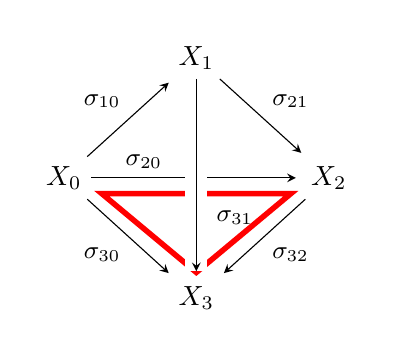
\begin{tikzpicture}[>=stealth,->,shorten >=2pt,looseness=.5,auto]
            \matrix[anchor=center, column sep=1cm, row sep=1cm] at (0,0)
            {
                                & \node(X_1) {$X_1$};   &                 \\
             \node(X_0) {$X_0$};     &                  & \node(X_2) {$X_2$};  \\
                                & \node(X_3) {$X_3$};   &                 \\
            };
            \draw[line width=2pt,color=red] (-1.2,-0.2) -- (1.2,-0.2) -- (0,-1.2) -- cycle;
            \begin{scope}[every node/.style={font=\small\itshape}]
                \draw (X_1) -- node [midway] {$\sigma_{21}$} (X_2);
                \draw (X_0) -- node [midway] {$\sigma_{10}$} (X_1);
                \draw (X_0) -- node [midway, swap] {$\sigma_{30}$}(X_3);
                \draw (X_0) -- node [near start] {$\sigma_{20}$}(X_2);
                \draw [-,line width=8pt,draw=white]
                (X_1) -- node [pos=0.7] {$\sigma_{31}$} (X_3);
                \draw (X_1) -- (X_3);
                \draw (X_2) -- node [midway] {$\sigma_{32}$} (X_3);
            \end{scope}
        \end{tikzpicture}              
    \]
    where the red triangle is not commuting a priori.
    The simplex gives the following identities
    \[
    \sigma_{30} = \sigma_{32} \circ \sigma_{20} \iff \sigma_{30} = \sigma_{32} \circ (\sigma_{21} \circ \sigma_{10}) = (\sigma_{32} \circ \sigma_{21}) \circ \sigma_{10} = \sigma_{31} \circ \sigma_{10} = \sigma_{30}
    \]
    which yields the commutativity of the bottom simplex.
\end{proof}

\begin{prop}
    Let $\mathcal{C} \in \Cat $. Then the following are equivalent:
    \begin{enumerate}
        \item 
        $\mathcal{C}$ is a groupoid,
        \item 
        $N(\mathcal{C})$ is a Kan complex.
    \end{enumerate}
\end{prop}

\begin{proof}
    "$2) \implies 1)$" 
    Let $f\colon X \to Y$ be a morphism in $\mathcal{C}$. 
    The horns 
    \[
    \begin{tikzcd}
        &
        Y
        \arrow[rd, dashed, "\exists g"]
        &\\
        X
        \arrow[ru, "f"]
        \arrow[rr,"1_X"']
        &
        &
        X
    \end{tikzcd}
    \qquad
    \begin{tikzcd}
        &
        X
        \arrow[rd, "f"]
        &\\
        Y
        \arrow[ru, dashed, "\exists h"]
        \arrow[rr,"1_Y"']
        &
        &
        Y
    \end{tikzcd}
    \]
    extend to 2-simplices of $N(\mathcal{C})$ since $N(\mathcal{C})$ is a Kan complex.
    So we get that $gf=\id_X$ and $fh=\id_Y$.
    Thus $\mathcal{C}$ is a groupoid.
    "$1) \implies 2)$"
    We already know that $N(\mathcal{C})$ is an inner Kan complex.
    "$1) \implies 2)$"
    We already know that $N(\mathcal{C})$ is an inner Kan complex.
    It is enough to consider the cases $n=2$, $k=0,2$ and $n=3$ $k=0,3$ by 2-coskeletality of $N(\mathcal{C})$.
    For $n=2$ and $k=0$ we have that the diagram 
    \[
    \begin{tikzcd}
        &X_1&\\
        X_0
        \arrow[ru, "\sigma_{10}"]
        \arrow[rr, "\sigma_{20}"']
        &&
        X_2
    \end{tikzcd}
    \]
    in $\mathcal{C}$, extends to 
    \[
    \begin{tikzcd}
        &X_1
        \arrow[rd, dashed, "\sigma_{20} \circ \sigma_{10}^{-1}"]
        &\\
        X_0
        \arrow[ru, "\sigma_{10}"]
        \arrow[rr, "\sigma_{20}"']
        &&
        X_2
    \end{tikzcd}
    \]
    where $\sigma_{20} \circ \sigma_{10}^{-1}$ exists since $\mathcal{C}$ is a groupoid.
    The case for $k=2$ is done analogously.
    For $n=3$ and $k=2$, consider the following 2-simplex
    \[
        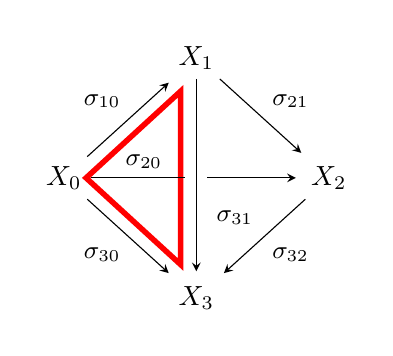
\begin{tikzpicture}[>=stealth,->,shorten >=2pt,looseness=.5,auto]
            \matrix[anchor=center, column sep=1cm, row sep=1cm] at (0,0)
            {
                                & \node(X_1) {$X_1$};   &                 \\
             \node(X_0) {$X_0$};     &                  & \node(X_2) {$X_2$};  \\
                                & \node(X_3) {$X_3$};   &                 \\
            };
            \draw[line width=2pt,color=red] (-0.2,1.1) -- (-0.2,-1.1) -- (-1.4, 0) -- cycle;
            \begin{scope}[every node/.style={font=\small\itshape}]
                \draw (X_1) -- node [midway] {$\sigma_{21}$} (X_2);
                \draw (X_0) -- node [midway] {$\sigma_{10}$} (X_1);
                \draw (X_0) -- node [midway, swap] {$\sigma_{30}$}(X_3);
                \draw (X_0) -- node [near start] {$\sigma_{20}$}(X_2);
                \draw [-,line width=8pt,draw=white]
                (X_1) -- node [pos=0.7] {$\sigma_{31}$} (X_3);
                \draw (X_1) -- (X_3);
                \draw (X_2) -- node [midway] {$\sigma_{32}$} (X_3);
            \end{scope}
        \end{tikzpicture}              
    \]
    which gives the following chain of identities:
    \[
    \sigma_{31} \circ \sigma_{10}= \sigma_{32} \circ \sigma_{21} \circ \sigma_{10} = \sigma_{32} \circ \sigma_{20} = \sigma_{30}
    \]
\end{proof}

Lecture 21.11

\begin{exmp}
    \begin{enumerate}
        \item 
        For all $X \in \Top$, $\Sing(X) \in \SetD$ is a Kan complex.
        \item 
        For all $\mathcal{C} \in \Cat$, $N(\mathcal{C})$ is an inner Kan complex.
        \item 
        $N(\mathcal{C)}$ is a Kan complex if and only if $\mathcal{C}$ is a groupoid.
        \item 
        For all $n\geq 0$, $\Delta^n=N([n])$ is an inner Kan complex and furthermore $\Delta^n$ is a Kan complex if and only if $n=0$.
        \item 
        If $M$ is a monoid then $N(BM)$ is an inner Kan complex and furthermore $N(BM)$ is a Kan complex if and only if $M$
    \end{enumerate}
\end{exmp}

\begin{defi}
    The category of simplicial groups is $\Fun(\Delta^{\op},\Grp)$. 
    Thus $X \in \Fun(\Delta^{\op},\Grp)$ consists of the following data:
    \begin{itemize}
        \item 
        For all $n\geq 0$ a group $X_n$ with a neutral element $e_n\in X_n$.
        \item 
        For all $0 \leq i \leq n$
        \begin{tabular}{c}
              $d_i\colon X_n \to X_{n-1}$ face map \\
              $s_i\colon X_n \to X_{n+1}$ degeneracy map,
        \end{tabular}
        satisfy the simplicial identities and are group homomorphisms.
    \end{itemize}
\end{defi}

\begin{prop}
    Let $X$ be a simplicial group. 
    Then the underlying simplicial set of $X$ is a Kan complex.
\end{prop}

\begin{proof}
    The case $n=1$ is trivial.
    We illustrate the argument for $n=2$ and $k=1$.
    Suppose given a horn 
    \[
    \begin{tikzcd}
        &
        x_1
        \arrow[rd, "x_{21}"]
        & \\
        x_0
        \arrow[ru, "x_{10}"]
        \arrow[rr, dashed, "\exists w"']
        &&
        x_2
    \end{tikzcd}
    \]
    Form the degenerate $2$-simplex $y \eqqcolon s_0(x_{21})$
    \[
    \begin{tikzcd}
        x_1
        \arrow[rd, "x_{21}"]
        &
        \\
        x_1
        \arrow[u, dashed, "1_{x_1}"]
        \arrow[r, "x_{21}"']
        &
        x_2
    \end{tikzcd}
    \]
    Let $z \coloneqq d_2(y) = 1_{X_1} \in X_1$.
    Consider now $s_1(x_{10}z^{-1})=s_1(x_{10}d_2(y)^{-1})=d_2(y^{-1})$.
    \[
    s_1(x_{10}z^{-1}):
    \begin{tikzcd}
        &
        x_1x_1^{-1}=e_0
        \arrow[rd, "1_{e_0}=s_0(e_0)=e_1"]
        &
        \\
        x_0x_1
        \arrow[ru, "x_{10}1_{x_1}^{-1}"]
        \arrow[rr, "x_{10}1_{x_1}^{-1}"']
        &&
        x_1x_1^{-1}=e_0
    \end{tikzcd}
    \]
    Let $w \coloneqq s_1(x_{10}z^{-1})y\in x_2$ and we get the chain of equalities
    \[
        d_0(w)=d_0((s_1(x_{10}z^{-1}))y)=d_0(s_1(x_{10}z^{-1}))d_0(y)=e_1x_{21}=x_{21}
    \]
    as well as 
    \[
    d_2(w)=d_2(s_1(x_0z^{-1}))d_2(y)=(x_{10}1_{x_1}^{-1})1_{x_1}=x_{10}e_1=x_{10}
    \]
    For the general case, consider a horn 
    \[
    (x_0,x_1,\dotsc, x_{k-1},\bullet,x_{k+1},\dotsc,x_n) 
    \]
    in $X$. Where $x_i \in X_{n-1}$ and $ d_i(x_j)=d_{j-1}(x_i)$ for $i<j$ and $i,j \neq k$.
    Suppose that there exists a $y \in X_n$ such that for all $ 0 \leq i < k$ and for all $l \leq i \leq n$.
    Then $w \coloneqq s_{l-2}(x_{l-1}\dotsm d_{l-1}(y)^{-1})y$ satisfies $d_i(w)=x_i$ for all $0 \leq i <k$ and all $l-1\leq i \leq n$.
\end{proof}

Recall the Dold-Kan correspondence.
\[
\begin{tikzcd}
    \tau \colon \Ab_{\Delta}
    \arrow[d, "\text{forgetfull}"']
    \arrow[r,"\sim"]
    &
    \Ch_{\leq} (\Ab)\colon Dk
    \arrow[l]
    \arrow[d, hook]
    &
    \\
    \SetD
    &
    \Ch(\Ab)
    \arrow[r,"\gamma"]
    &
    D(\Ab)
\end{tikzcd}
\]

\begin{prop}
    Let $X$ be a Kan complex ($X \in \SetD$).
    Then $x,y \in X_0$ satisfy $[x]=[y]$ in $\pi_0(X)$ if and only if there exists a $\sigma \in X_1$ such that $d_0(\sigma)=y$ and $d_1(\sigma)=x$.
\end{prop}

\begin{proof}
    At first, when there is a $\sigma$ that relates $X$ to $Y$ we can complete this to 1-simplex
    \[
    \begin{tikzcd}
        &
        Y
        \ar[rd, "d_0(\tau)"]
        &
        \\
        X
        \ar[ru,"\sigma"]
        \ar[rr,"1_X"']
        &&
        X
    \end{tikzcd}
    \]
    and obtain $d_0(\tau)$ that relates $Y$ to $X$.
    Also if $X$ relates to $Y$ and $Y$ relates to $Z$, we obtain a $2$-simplex
    \[
    \begin{tikzcd}
        &
        Y
        \ar[rd, "\tau"]
        &
        \\
        X
        \ar[ru,"\sigma"]
        \ar[rr,"d_1(\alpha)"']
        &&
        Z
    \end{tikzcd}
    \]
    where $d_1(\alpha)$ relates $X$ to $Z$.
\end{proof}

\subsection{Exercises}

\begin{Exercise}
    \begin{enumerate}[label=(\alph*)]
        
        \item 
        Show that for $ n \in \mathbb{N}_0 $ we have $ \bold{sk}_n ( \Delta^{n+1} ) \cong \partial \Delta^{n+1}$.
    
        \item 
        Show that for every horn $ \Lambda_k^m $ we have that 
        \[
            \bold{sk_n} ( \Lambda_k^m ) \cong 
            \begin{cases}
                \Lambda_k^m &\text{ if } m \leq n+1
                \\
                \bold{sk}_n ( \Delta^m ) &\text{ if } m > n+1
            \end{cases}
        \]
        for $ 0 \leq k \leq m \in \mathbb{ N }_+$.
    
        \item 
        Show that for a Kan comlex $ K $ and any $ n \in \mathbb{N}_0 $, the $ n $-coskeleton $\bold{cosk}_n ( K ) $ is a Kan complex.
        
    \end{enumerate}
\end{Exercise}

\begin{Exercise}
    \begin{enumerate}[label=(\alph*)]
        \item 
        Show that the class of Kan complexes and the class of inner Kan complexes are closed under set indeced products.
    
        \item 
        Show that a set indexed product of connected Kan complexes is connected.
    
        \item 
        Give an example that an infinite product of connected inner Kan complexes is not necessarily connected. 
        ( Recall that the nerve of a category is an inner Kan complex.)
    \end{enumerate}
\end{Exercise}
\section{Fundamental groupoid revisited}

Recall the adjunction 
    \begin{tikzcd}
         \Set_{\Delta}
        \arrow[r, shift left, "\tau"]
        &
        \Gpd
        \arrow[l, shift left, "N"]
    \end{tikzcd}
and suppose that $X \in \Set_{\Delta}$ is a Kan complex.

\begin{construction}

The homotopy category of $X$ is called $\H0(X)$ is defined as follows:
\begin{itemize}
    \item 
    $\Ob(\H0(X))=X_0$
    \item 
    $\hom_{\H0(X)}(X,Y) = \{f \in X_1 \mid d_1(f)=X , d_0(f)=y \} / \sim$
\end{itemize}

Recall that a $2$-simplex of $X$
\[
\begin{tikzcd}
    &
    Y
    \arrow[rd,"g"]
    &\\
    X
    \arrow[ru, "f"]
    \arrow[rr,"h"']
    &
    &
    Z
\end{tikzcd} 
\]
should be a "witness" of the fact the $h$ is a composition of $f$ and $g$.
\end{construction}

\begin{problem}
    Why are there different choices of relation $\sim$?
    Given as follows
    \[
    \begin{tikzcd}
        &
        X
        \arrow[rd,"f"]
        &\\
        X
        \arrow[ru, "1_X"]
        \arrow[rr,"g"']
        &
        &
        Y
    \end{tikzcd} 
    = f \sim_1 g
    \qquad
    \begin{tikzcd}
        &
        Y
        \arrow[rd,"1_Y"]
        &\\
        X
        \arrow[ru, "f"]
        \arrow[rr,"g"']
        &
        &
        Y
    \end{tikzcd} 
    = f \sim_2 g
    \]
    \[
    \begin{tikzcd}
        &
        X
        \arrow[rd,"g"]
        &\\
        X
        \arrow[ru, "1_X"]
        \arrow[rr,"f"']
        &
        &
        Y
    \end{tikzcd} 
    = f \sim_3 g
    \qquad
    \begin{tikzcd}
        &
        Y
        \arrow[rd,"1_Y"]
        &\\
        X
        \arrow[ru, "g"]
        \arrow[rr,"f"']
        &
        &
        Y
    \end{tikzcd} 
    = f \sim_4 g
    \]
    where $1_X\coloneqq s_0(X)$. 
    What remains to be shown is that all these are equivalence relations and are in fact the same.
\end{problem}

Lecture 26.11

\begin{prop}
    The four relations above are the same and are equivalence relations.
\end{prop}

\begin{proof}
    We show $(f \sim_3 g \implies f \sim_1 g)$, thus let 
    \[
    \begin{tikzcd}
        &
        X
        \arrow[rd,"g"]
        &\\
        X
        \arrow[ru, "1_X"]
        \arrow[rr,"f"']
        &
        &
        Y
    \end{tikzcd} 
    = \sigma \in X_2
    \]
    We can glue the following $2$-simplices 
    \[
    \begin{tikzcd}
        &
        X
        \arrow[rd,"1_X"]
        &\\
        X
        \arrow[ru, "1_X"]
        \arrow[rr,"1_X"']
        &
        &
        X
    \end{tikzcd} 
    =c^2(X)
    \qquad
    \begin{tikzcd}
        X
        \arrow[rr,"1_X"]
        \arrow[rd,"g"']
        &
        &
        X
        \arrow[ld, "g"]
        \\
        &
        Y
        &
    \end{tikzcd}
    =s_0(g)
    \]
    \[
    \begin{tikzcd}
        X
        \arrow[dd,"f"']
        \arrow[rd,"1_X"]
        &
        \\
        &
        X
        \arrow[ld,"g"]
        \\
        Y
    \end{tikzcd}
    =\sigma
    \]
    to obtain a $3$-horn
    \[
    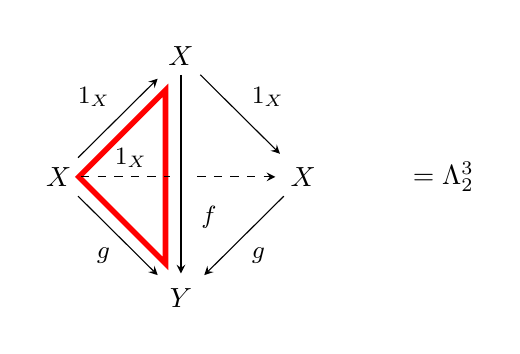
\begin{tikzpicture}[>=stealth,->,shorten >=2pt,looseness=.5,auto]
            \matrix[anchor=center, column sep=1cm, row sep=1cm] at (0,0)
            {
                                & \node(X_1) {$X$};   &                 &\\
             \node(X_0) {$X$};     &                  & \node(X_2) {$X$};& \node(X_24) {$=\Lambda_2^3$};  \\
                                & \node(X_3) {$Y$};   &                 &\\
            };
            \draw[line width=2pt,color=red] (-1.2,1.1) -- (-1.2,-1.1) -- (-2.3, 0) -- cycle;
            \begin{scope}[every node/.style={font=\small\itshape}]
                \draw (X_1) -- node [midway] {$1_X$} (X_2);
                \draw (X_0) -- node [midway] {$1_X$} (X_1);
                \draw (X_0) -- node [midway, swap] {$g$}(X_3);
                \draw [dashed] (X_0) -- node [near start] {$1_X$}(X_2);
                \draw [-,line width=8pt,draw=white]
                (X_1) -- node [pos=0.7] {$f$} (X_3);
                \draw (X_1) -- (X_3);
                \draw (X_2) -- node [midway] {$g$} (X_3);
            \end{scope}
    \end{tikzpicture} 
    \]
    The red $2$-simplex is exactly the one of the equivalence relation $f \sim_1 g$. 
    Since $X$ is an inner Kan complex by assumption, we have the desired horn extension.
    The other direction were part of an exercise and will be included here eventually.
    What remains to be shown, is that it is an equivalence relation.
    \begin{itemize}
        \item 
        (Reflexivity) 
        Let $X \xrightarrow{f} Y$ be in $X_1$, then we have the 2-simplex
        \[
        \begin{tikzcd}
            &
            X
            \arrow[rd,"f"]
            &\\
            X
            \arrow[ru, "1_X"]
            \arrow[rr,"f"']
            &
            &
            Y
        \end{tikzcd} 
        \]
        which means that $\sim$ is associative.
        \item 
        (Symmetry)
        We have the following chain of equivalences
        \[
        f\sim g \iff f\sim_1 g \iff f \sim_3 g \iff g \sim_1f \iff g \sim f
        \]
        \item 
        (Transitivity)
        Let $f\sim g$ and $g \sim h$.
        Consider the following diagrams
        \[
        \begin{tikzcd}
            &
            X
            \arrow[rd, "f"]
            &
            \\
            X
            \arrow[rr, "g"]
            \arrow[ru, "1_X"]
            \arrow[rd, "h"']
            &
            &
            Y
            \arrow[ld,"1_Y"]
            \\
            &
            Y
            &
        \end{tikzcd}
        \qquad
        \begin{tikzcd}
            X
            \arrow[dd, "f"']
            \arrow[rd, "f"]
            \\
            &
            Y
            \arrow[ld, "1_Y"]
            \\
            Y
        \end{tikzcd}
        \] which glued at $1_Y$ and $f$ result in the following horn
        \[
        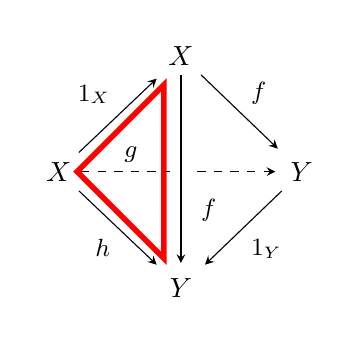
\begin{tikzpicture}[>=stealth,->,shorten >=2pt,looseness=.5,auto]
            \matrix[anchor=center, column sep=1cm, row sep=1cm] at (0,0)
            {
                                & \node(X_1) {$X$};   &                 \\
             \node(X_0) {$X$};     &                  & \node(X_2) {$Y$};  \\
                                & \node(X_3) {$Y$};   &                 \\
            };
            \draw[line width=2pt,color=red] (-0.2,1.1) -- (-0.2,-1.1) -- (-1.3, 0) -- cycle;
            \begin{scope}[every node/.style={font=\small\itshape}]
                \draw (X_1) -- node [midway] {$f$} (X_2);
                \draw (X_0) -- node [midway] {$1_X$} (X_1);
                \draw (X_0) -- node [midway, swap] {$h$}(X_3);
                \draw [dashed] (X_0) -- node [near start] {$g$}(X_2);
                \draw [-,line width=8pt,draw=white]
                (X_1) -- node [pos=0.7] {$f$} (X_3);
                \draw (X_1) -- (X_3);
                \draw (X_2) -- node [midway] {$1_Y$} (X_3);
            \end{scope}
    \end{tikzpicture}
    \]
    By the horn filling property of the inner Kan complex for a 3-horn at position 2 we get the desired $f \sim g$.
    \end{itemize}
\end{proof}

\begin{prop}
    The composition law in $\H0(X)$ is well defined, unital and associative.
\end{prop}

\begin{proof}
    Suppose that $f \sim f'$. 
    From now on we write $gf \sim h$ to mean that there exists a 2-simplex
    \[
    \begin{tikzcd}
        &
        Y
        \arrow[rd,"g"]
        &\\
        X
        \arrow[ru, "f"]
        \arrow[rr,"h"']
        &
        &
        Z
    \end{tikzcd}   
    \in X_2
    \]
    We prove that if $gf \sim h$, $gf' \sim h'$ and $gf' \sim h$ it follows that $h \sim h'$. 
    So consider the corresponding 2-simplices
    \todo{i am too lazy to do the "assemble the obvious simplex proves" right now, soooo fuck you future Vincent suuuckkaaaaa}
\end{proof}

\begin{rmk}
    \todo{what does this remark mean?}
    \begin{tikzcd}
        &&Z
    \end{tikzcd}
    $\H0 (X)$ is a well defined category when $X$ is an inner Kan complex.
\end{rmk}

\begin{prop}
    Let $X \in \SetD$ be $X$ a Kan complex, then $\H0 (X)$ is a groupoid.
\end{prop}

\begin{proof}
    Let $f \in \H0(X)$ be a morphism. 
    Consider the simplex 
    \begin{tikzcd}
        & 
        X
        \arrow[rd, "f"]
        &
        \\
        Y
        \arrow[rr, "1_Y"']
        \arrow[ru, dashed, "\exists g"]
        &&
        Y
    \end{tikzcd}
\end{proof}

\begin{cor}
    Let $X \in \SetD$ be a Kan complex, then $L \H0(X) \cong \H0(X)$.
\end{cor}

\begin{proof}
     Consider the adjunction 
     \[
     \begin{tikzcd}
        \Cat
        \arrow[r, shift left, "L"]
        &
        \Gpd 
        \arrow[l, shift left, "y'"]
    \end{tikzcd}
     \]
     Then the counit $\eta$ of the adjunction is the desired isomorphism.
     \todo{details}
\end{proof}

\begin{prop}
    Let $X \in \SetD$ be an inner Kan complex, then $H_0(X) \cong \tau X$.
\end{prop}

\begin{proof}
    Let $\mathcal{D} \in \Cat$, since $N(\mathcal{D}) \in \SetD$ is $2$-coskeletal, we have a natural bijection.
    \[
    \Hom_{\SetD}(X, N( \mathcal{D})) \isomorphism \Hom_{\SetD}(\tru_2X,\tru_2(N(\mathcal{D}))
    \]
    Consider a morphism $\tru_2(X) \xrightarrow{f} \tru_2(N(\mathcal{D}))$ given by
    \[
    \begin{tikzcd}
        \tru_2
        \arrow[d,"f"]
        &
        X\colon \dotsc 
        &
        X_2
        \arrow[r, altstackar=5]
        \arrow[d,"f_2"]
        &
        X_1
        \arrow[r,altstackar=3]
        \arrow[d,"f_1"]
        &
        X_0=\Ob(\Ho(X))
        \arrow[d,"f_0"]
        \\
        \tru_2(N(\mathcal{D}))
        &
        N(\mathcal{D})\colon \dotsc 
        &
        N(\mathcal{D})_2
        \arrow[r, altstackar=5]
        &
        N(\mathcal{D})_1
        \arrow[r,altstackar=3]
        &
        N(\mathcal{D})_0=\Ob(\mathcal{D})
    \end{tikzcd}
    \]
    Note that $N(\mathcal{D})_1=\Mor( \mathcal{D} )$.
    We have for any $\alpha \in X_1$ that $f_0(d_0(\alpha)) = \text{target} (f_1(\alpha))$ and that for any $d_1(\alpha) \xrightarrow{\alpha}d_0(\alpha)$ that $f_0(d_1(\alpha))= \text{source}(\alpha)$.
    Now for 2-simplices we have
    \[
    \alpha \sim \beta
     \begin{tikzcd}
        &
        x
        \arrow[rd,"\alpha"]
        &\\
        x
        \arrow[ru, "1_x"]
        \arrow[rr,"\beta"']
        &
        &
        y
    \end{tikzcd}   
    \xmapsto{f_2}
    \begin{tikzcd}
        &
        f_0(x)
        \arrow[rd,"f_1(\alpha)"]
        &\\
        f_0(x)
        \arrow[ru, "\id_{f_0(x)}"]
        \arrow[rr,"f_1(\beta)"']
        &
        &
        f_0(y)
    \end{tikzcd}
    \]
    Thus $f_1(\alpha)=f_1(\beta)$ which results in 
    \[
    \Hom_{\Set_{\Delta}}(\tr_2(X), \tr_2(N(\mathcal{D})) \isomorphism \Hom_{\Cat}(\Ho(X), \mathcal{D})
    \]
\end{proof}

\begin{cor}
    Let $X \in \Set_{\Delta}$ be a Kan complex. 
    Then $\pi_1(X)=\Ho(X)$ and for all $x \in X_0$ it holds that
    $\pi_1(X,x) \isomorphism \Hom_{\Ho(X)}(x,x)$.
\end{cor}

\begin{proof}
    We know that 
    \[
    \pi_1(X,x) = \Hom_{\pi_1(X)}(x,x) \isomorphism \Hom_{\Ho(X)}(x,x)
    \]
    as well as 
    \[
    \pi_1(X)=L(\tau X) \isomorphism L(\Ho(X)) \isomorphism \Ho(X).
    \]
    \todo{check this proof}
\end{proof}
\section{Kan Fibrations}

Aim: Formalize the idea of a "family of Kan complexes parametrized by a simplicial set", i.e. suitable morphisms $X \xrightarrow{p} Y$ in $\Set_{\Delta}$ whose fibres are Kan complexes.
That is we have a pullback diagram
\[
\begin{tikzcd}
    X_y
    \arrow[d]
    \ar[r]
    &
    X
    \ar[d,"p"]
    \\
    \Delta^0
    \ar[r,"y"]
    &
    Y    
\end{tikzcd}
\]

\underline{Terminology}:
Let $ L \xrightarrow{i} K$ and $ X \xrightarrow{p} Y$ be morphisms.
We say that ($ i \lift{} p$) $i$ has the left lifting property with respect to $p$ (equivalently $p$ has the right lifting property with respect to $i$).
If there exists for every $L \xrightarrow{f} X$ and $K \xrightarrow{g}Y$ a morphism $h:K \to X$ such that the following diagram commutes
\[
\begin{tikzcd}
    L
    \arrow[d,"i"]
    \ar[r, "f"]
    &
    X
    \ar[d,"p"]
    \\
    K
    \ar[ru,"h"]
    \ar[r,"g"]
    &
    Y    
\end{tikzcd}
\]
Let $X \in \SetD$ be a Kan complex. 
Then 
\[
\{ \Lambda_k^n \to \Delta^n \mid n\geq 1 ,0 \leq k \leq n \} \lift{} (X \to \Delta^0)
\]
is given by 
\[
\begin{tikzcd}
    \Lambda_k^n
    \arrow[d,"\iota"']
    \ar[r, "\sigma"]
    &
    X
    \ar[d,"!"]
    \\
    \Delta^n
    \ar[ru,"\Tilde{\sigma}"]
    \ar[r,"!"']
    &
    \Delta^0
\end{tikzcd}
\]

\begin{defi}
    A morphism $X \xrightarrow{p} Y$ is a Kan fibration if 
    \[
    \{ \Lambda_k^n \to \Delta^n \mid n\geq 1 ,0 \leq k \leq n \} \lift{} (X \xrightarrow{p} Y)
    \]
\end{defi}

\begin{rmk}
    We may as well write $X \xrightarrow{p} Y \in \{ \Lambda_k^n \to \Delta^n \mid n\geq 1 , 0 \leq k \leq n\}^{\lift{}}$.
\end{rmk}

\begin{lem}
    Let $i \lift{} p$ and
    \[
    \begin{tikzcd}
        X'
        \arrow[d,"p'"]
        \ar[r]
        &
        X
        \ar[d,"p"]
        \\
        Y'
        \ar[r,"v"]
        &
        Y    
    \end{tikzcd}
    \]
    be a pullbacksquare, then $i \lift{} p'$.
\end{lem}

\begin{proof}
    Consider the diagram
    \[
    \begin{tikzcd}
        L
        \ar[r,"f"]
        \ar[d,"i"']
        &
        X'
        \arrow[d,"p'" pos=0.65]
        \ar[r, "u"]
        &
        X
        \ar[d,"p"]
        \\
        K
        \arrow[r,"g"']
        \ar[rru, dashed, "r" pos= 0.4]
        \ar[ru, dashed, "h"]
        &
        Y'
        \ar[r,"v"']
        &
        Y    
    \end{tikzcd}
    \]
    where $r$ exists since $i$ has the left lifting property with respect to $p$ and $h$ exists by the universal property of the pullback.
    Now $u \circ h \circ i = r \circ i = u \circ f$ and $p' \circ h \circ i = q \circ i = p' \circ f$, since the  morphism given by the pullback is unique we get that $h \circ i = f$.
\end{proof}

Lecture 3.12 

Formalise the notion of a locally constant family of Kan complexes relative to a base simplicial set.

\begin{defi}
    Let $X \xrightarrow{p} Y$ be a Kan fibration. 
    By the preceding theorem, we get that for every $y\in Y_0$ the fibre $X_y$ is a Kan complex. 
    Now consider $\Delta^0$ as the simplicial set where $\Delta^0_n=\Hom_{\SetD}([n],[0])=\{[n] \to [0]\}$ is the unique map into the final object.
    We have the constant map 
\todo{alot missin here}
\end{defi}

\begin{prop}
\label{comp_Kan_fib}
    Let $L \xrightarrow{i} K$ be a morphism and suppose that $X \xrightarrow{p} Y$, $Y \xrightarrow{g} Z$ have the right lifting property with respect to $i$, then the composition $g \circ p$ has the right lifting property with respect to $i$.
\end{prop}

\begin{proof}
    This is just a simple matter of writing down the square for $g$ and using the obtained morphism to write down the square $p$ obtaining a morphism that fllfills the desired property.
\end{proof}

\begin{cor}
    Suppose that $X \xrightarrow{p} Y$ is a Kan fibration and $Y$ is a Kan complex, then $X$ is a Kan complex.
\end{cor}

\begin{proof}
    Since $X \xrightarrow{p} Y$ is a Kan fibration and $Y \to \Delta^0$ is a Kan fibration, we get by \cref{comp_Kan_fib} that $X \to \Delta^0$ is a Kan fibration, thus we get that $X$ is a Kan complex.
\end{proof}

\begin{prop}
    Let $X^{(i)} \xrightarrow{p^i} Y^{(i)}$ with $i \in I$ be a set indexed family of Kan fibrations.
    Then $\prod X^{(i)} \xrightarrow{\prod p^i} \prod Y^{(i)}$ is a Kan fibration.
\end{prop}

\begin{proof}
Consider the diagram arising from the assumptions
\[
    \begin{tikzcd}
        \Lambda_k^n
        \ar[r,"\sigma"]
        \ar[d,"\iota"]
        &
        \prod X^{(i)}
        \ar[d, "\prod p^i" pos=0.7]
        \ar[r, "\prod \pi_j"]
        &
        X^{(j)}
        \ar[d, "p^j"]
        \\
        \Delta^n
        \ar[ru, dashed, "\exists ?"]
        \ar[rru, dashed, "h_j" pos=0.4]
        \ar[r, "\tau"']
        &
        \prod Y^{(i)}
        \ar[r, "\pi_j"']
        &
        Y^{(j)}
    \end{tikzcd}
\]
Since $p_j$ is a Kan fibration, there exists $h_j \colon \Delta^n \to X^{(j)}$ such that 
$\begin{cases}
    p_jh_j=\pi_j\tau\\
    h_j\iota = \pi_j \sigma_j.
\end{cases}$
    The universal property of the product gives $h \colon \Delta^n \to \prod X^{(i)}$ such that $\pi_j \circ h = h_j$.
    Now we have that $\pi_j(h \circ \iota ) = h_j \circ \iota = \pi_i \circ \sigma$ and thus $h \circ \iota = \sigma$ as well as $\pi_j(\prod {p_i} \circ h) = p_j \circ \pi_j \circ h = p_j h_j = \pi_j \tau$ and thus $\prod p_i \circ h = \tau$, where the equalities follow from the uniqueness of the morphism given by the pullback.
\end{proof}

\begin{prop}
    Let $\dotsc \to X^{(n)} \xrightarrow{p_n} \dotsc \to X^{(1)} \xrightarrow{p_1}X^{(0)}$ be a "tower" of Kan fibrations, that is for all $i, p_i$ is a Kan fibration.
    Then $X^{\infty} \coloneqq \lim X^{(n)} \xrightarrow{\pi_0} X^{(0)}$ is a Kan fibration. 
\end{prop}

\begin{proof}
    Consider the diagram 
\[
\begin{tikzcd}
    \Lambda_k^n
    \arrow[d,"\iota"']
    \ar[r, "\sigma"]
    &
    X^{(\infty)}
    \ar[d,"\pi_0"]
    \\
    \Delta^n
    \ar[ru, dashed, "\exists ?"]
    \ar[r,"\tau"']
    &
    X^{(0)}
\end{tikzcd}
\]
The idea is to construct a cone of the tower with apex $\Delta^n$ and then use the universal property $X^\infty$.
\todo{finish this ya lazy bombaclat}
\end{proof}

%done

\section{Anodyne extensions}

\begin{defi}
    We say that a class $\mathcal{M}$ of morphisms in $\mathcal{C}$ is a \underline{saturated class} if 
    \begin{enumerate}
        \item 
        $\mathcal{M}$ contains all isomorphisms,
        \item 
        $\mathcal{M}$ is closed under compositions,
        \item
        if $i:L \to K$ is in $\mathcal{M}$ then so is the pushout $i'$ given by the pushout diagram 
        \[
        \begin{tikzcd}
            L
            \arrow[d,"i"]
            \ar[r,"\sigma"]
            &
            L'
            \ar[d,"i'"]
            \\
            K
            \ar[r]
            &
            K'   
        \end{tikzcd}
        \]
        \item
        $\mathcal{M}$ is closed under coproducts and
        \item 
        for any sequence of objects and morphism 
        \[
        L^{(0)} \to L^{(1)} \to L^{(2)}\to \dotsc
        \]
        in $\mathcal{M}$, the morphism $L^{(0)} \to L^{(\infty)}=\colim L^{(n)}$ is in $\mathcal{M}$.
    \end{enumerate}
    We say that $\mathcal{M}$ is a saturated class of monomorphisms if all $i \in \mathcal{M}$ are monomorphisms.
\end{defi}

\begin{defi}
    The \underline{saturation} of a class of monos is the intersection of all such containing it. We write $\overline{\mathcal{M}}$ for its saturation.
\end{defi}

\begin{defi}
    The class of anodyne extensions is $\overline{\{ \Lambda_k^n \xrightarrow{i_k^n} \Delta^n \mid 1 \leq n ,0 \leq k \leq n \}}=\An$.
\end{defi}

\begin{rmk}
    The term anodyne extensions translates to something like harmless extensions.
\end{rmk}

\begin{prop}
    The class $\An^{\lift{}}$ is equal to the Kan fibrations.
\end{prop}

\begin{proof}
    $(\subseteq)$ Let $p \in \An^{\lift{}}$, then for all $n\geq 0$ there exists $0 \leq k \leq  n$ such that $i_{n,k} \lift{} p: p \in \KanFib$

    $(\supseteq)$ Consider $\prescript{\lift{}}{}{\KanFib}$, this is a saturated class. 
    By unitality of $\An \subseteq \prescript{\lift{}}{}{\KanFib}$ it holds that for all $i \in  \An$ and all $p \in \KanFib$ $i\lift{}p $ which means that for all $p \in \KanFib$ we have that $p \in \An^{\lift{}}$
\end{proof}

\subsection{Exercises}

\begin{Exercise}
    
We define the class of trivial Kan fibrations to be $ r ( \{ \partial \Delta^n \to \Delta^n \mid n \in \mathbb{ N }_0 \} ) $ in $ \SetD $.
Furthermore, let $ \mathcal{ F } $ be the smallest saturated class containing all boundary inclusions $ \{ \partial \Delta^n \to \Delta^n \mid n \in \mathbb{ N }_0 \} $.

\begin{enumerate}[label=(\alph*)]
    \item 
    Show that $ r ( \mathcal{ F } ) $ is the class of trivial Kan fibrations.

    \item 
    Show that $ \mathcal{ F } $ contains all monomorphisms. Proceed as follows.

    \begin{itemize}
        \item 
        For a fixed monomorphism $ \iota : X \to Y $ construct a filtration of $ Y $ by $ X \cup \bold{sk_{n-1}} ( Y ) $ starting with $ X = X \cup \bold{sk_{-1}}( Y ) $, similar to the skeletal filtration from Exercise 7.2. 
        Here $ X \cup \bold{sk_n} ( Y ) $ is defined as pushouts of $ \bold{ sk_n } ( Y ) $ and the image of $ \iota $ along their intersection.

        \item 
        Observe that $ \iota $ is the transfinite composition of this filtration.

        \item 
        Show that the morphisms $ X \cup \bold{sk_{n-1]}}( Y ) \to X \cup \bold{ sk_n }( Y ) $ is pushout of morphisms in $ \mathcal{ F } $ for all $ n \in \mathbb{ N }_0 $ by construction a similar pushout diagram as for the skeletal filtration.
    \end{itemize}

    \item 
    Deduce that $\mathcal{ F }$ is the class of monomorphisms.

    \item 
    Conclude that a trivial Kan fibration is a Kan fibration.
    
\end{enumerate}

\end{Exercise}

\begin{Exercise}
    
We have shown in the lecture that the saturated closure of the horn inclusions 
\[
    \mathcal{B}_1 
    \coloneqq 
    \{ \Lambda_k^n \subseteq \Delta^n \mid 0 \leq k \leq n \in \mathbb{ N }_+ \}
\]
agrees with the saturated closure of
\[
    \mathcal{B}_2
    \coloneqq
    \{ ( \Delta^1 \times \partial\Delta^n) \cup ( \{ \epsilon \} \times \Delta^n ) \subseteq ( \Delta^1 \times \Delta^n ) \mid n \in \mathbb{ N }_0 , \\epsilon \in \Delta_0^1 = \{ 0 , 1 \} \}.
\]
We call this class the anodyne extensions $ \bold{ An }$.
Show that $ \bold{ An } $ agrees with the saturated closure of 
\[
    \mathcal{ B }_3 
    \coloneqq
    \{ ( \Delta^1 \times X ) \cup ( \{ \epsilon \} \times Y ) \subseteq ( \Delta^1 \times Y ) \mid  \epsilon \in \Delta_0^1 = \{ 0 , 1 \} , X \to Y \text{ monomorphism } \}.
\]

\end{Exercise}




    
\include{Reminder: Function complexes}

% done

\section{Simplicial Homotopy}

Aim: Introduce the notion of homotopy between maps of simplicial sets.

\begin{defi}
    Let $f,g \colon K \to X$ be morphisms of simplicial sets
\end{defi}

A homotopy $h\colon f \to g$ is a morphism $\Delta^1 \times K \xrightarrow{h} X$ such that 
\[
\begin{tikzcd}
    \Delta^{\{0\}} \times K \cong K
    \ar[d, "i_0 \times \id"']
    \ar[dr, "f"]
    \\
    \Delta^1 \times K 
    \ar[r,"h"]
    &
    X
    \\
    \Delta^{\{1\}}\times K \cong K
    \ar[u,"i_1 \times \id"]
    \ar[ur, "g"']
\end{tikzcd}
\]

\begin{exmp}
    Let $x,y \colon \Delta^0 \to X$ be vertices of $X$. 
    A homotopy $h\colon x \to y$ is a map $h$ such that
    \[
    \begin{tikzcd}
        \Delta^{\{0\}} \times K \cong K
        \ar[d, "i_0 \times \id"']
        \ar[dr, "x"]
        \\
        \Delta^1 \times K 
        \ar[r,"h"]
        &
        X
        \\
        \Delta^{\{1\}}\times K \cong K
        \ar[u,"i_1 \times \id"]
        \ar[ur, "y"']
    \end{tikzcd}
    \]
    that is $h \in X_1$ such that $d_1(h)=x$ and $d_0(h)=y$.
\end{exmp}

\subsection{Adjoint description of homotopy}
Let $f,g \in \Hom(K,X) = \underline{\Hom}(K,X)_0$ and $h\colon f\mapsto g$, that is $h \in \Hom(\Delta^1 \times K, X) = \underline{\Hom}(K,X)_1$ such that $d_1(h)=f$ and $d_0(h)=g$.

\underline{Upshot} Homotopy of maps $K \to X$ is an equivalence relation if $\underline{\Hom}(K,X)$ is a Kan complex.
So take the following lifting problem

\[
    \begin{tikzcd}
        \Lambda_k^n
        \ar[r,"\sigma"]
        \ar[d,"\iota"]
        &
        \underline{\Hom(K,X)}
        \ar[d]
        \\
        \Delta^n
        \ar[ur, dashed, "\exists"]
        \ar[r]
        &
        \Delta^0
    \end{tikzcd}
\]
which equates to the following lifting problem due to the adjunction of the inner hom and the product.
\[
\begin{tikzcd}
    \Lambda^n_k \times K
    \ar[r, " \overline{\sigma} "]
    \ar[d, " i \times \id_K"' ]
    &
    X
    \\
    \Delta^n \times K
    \ar[ru, dashed, " \overline{ \rho }"']
\end{tikzcd}
\]
If now $X$ were a Kan complex, then we would obtain a lift if $ i \times \id_K $ is an anodyne extension.

\begin{defi}
    Let $i\colon L \hookrightarrow K$ is a monomorphism in $\SetD$.
    Let $f,g \colon K \to X$ be such that $f \circ i = g \circ i$ we also write $(f_{\mid L}=g_{\mid L})$. A homotopy $h\colon f \to g $ (rel $L$) is a homtopy $h \colon f \to g$ such that 
    \[
    \begin{tikzcd}
        \Delta^1 \times L 
        \ar[r, "\pi_L"]
        \ar[dr,"1_{\alpha}"]
        \ar[d, "\id \times i"']
        &
        L
        \ar[d, "f_{\mid L} = \alpha = g_{\mid L}"]
        \\
        \Delta^1 \times K 
        \ar[r, "h"]
        &
        X
    \end{tikzcd}
    \]
    where $1_{\alpha}$ is given by $\Delta^1 \times L \xrightarrow{(!,\id_L)} \Delta^0 \times L \xrightarrow{\alpha}X$ and $!$ is the unique map into the terminal object.
\end{defi}

\subsection{Adjoint description of relative homotopy}

Consider the pullbackdiagram

\[
\begin{tikzcd}
    \Delta^1
    \ar[rd,"\Tilde{h}"]
    \ar[rrd,bend left,"h"]
    \ar[ddr, bend right]
    \\
    &
    \underline{\Hom}(K,X)_{\alpha}
    \ar[r]
    \ar[d]
    &
    \underline{\Hom}(K,X)
    \ar[d,"i^*"]
    \\
    &
    \Delta^0
    \ar[r,"\alpha"]
    &
    \underline{\Hom}(L,X)
\end{tikzcd}
\]

A morphism $\overline{h}$ into the fiber induces a homotopy $ h $ that is constant on $L$, thus this pullback gives us the construction of homotopy relative the simplical subset $L$.

We want that given a Kan complex $X$, to get that $ \underline{\Hom} ( K , X ) \xrightarrow{i^*} \underline{\Hom} ( L , X ) $ is a Kan fibration and finally get that $ \underline{ \Hom } ( K , X )_{\alpha} $ is a Kan complex and that homotopy ( rel $L$ ) is the equivalence relation on vertices of $ \underline{ \Hom } ( K , X )_{\alpha}$.

Rest is for now omitted since I cannot read my own notes.
Lecture 10.12

\begin{prop}
    The following classes have the same saturated closure
     \[
     \begin{tabular}{c}
          $B_1\coloneqq \{\Lambda_k^n \hookrightarrow\Delta^n \mid 0\leq n,0 \leq k \leq n \}$
          \\
          $B_2\coloneqq \{(\Delta^1 \times \partial \Delta^n) \cup(\Delta^{\{l\}} \times \Delta^n) \xhookrightarrow{i} \Delta^1 \times \Delta^n \mid 0 \leq n, l \in \{0,1\}\}$
          \\
          $B_3 \coloneqq
          \{ ( \Delta^1 \times L) \cup(\Delta^{\{0\}} \times K) \hookrightarrow \Delta^1 \times K \mid L \subseteq K \}$
     \end{tabular}
     \]
     where the product $\Delta^1 \times \Delta^n = N ( [1]) \times N([n]) \cong N ( [1] \times [n] )$ and $[1] \times [n] $ is given by the following diagram:
     \[
     \begin{tikzcd}
         00
         \ar[r]
         \ar[d]
         &
         01
         \ar[r]
         \ar[d]
         &
         \dotsc
         \ar[r]
         &
         0n
         \ar[d]
         \\
         10 
         \ar[r]
         &
         11
         \ar[r]
         &
         \dotsc
         \ar[r]
         &
         1n
     \end{tikzcd}
     \]
\end{prop}

As an example for $l=1$ and $n=2$ the domain of a morphism in $B_2$ is given by the following diagram, where the red triangle indicates 2-simplex with its interior removed.
\[
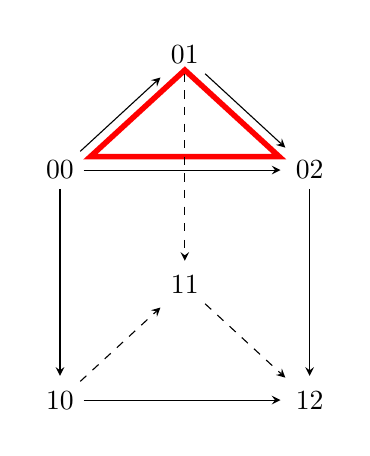
\begin{tikzpicture}[>=stealth,->,shorten >=2pt,looseness=.5,auto]
            \matrix[anchor=center, column sep=1cm, row sep=1cm] at (0,0)
            {
                                & \node(01) {$01$};   &                 \\
             \node(00) {$00$};     &                  & \node(02) {$02$}; \\
                                & \node(11) {$11$};   &                  \\
            \node(10) {$10$};    &                     & \node(12) {$12$}; \\ 
            };
            \draw[line width=2pt,color=red] (-1.2,0.9) -- (1.2,0.9) -- (0, 2) -- cycle;
            \begin{scope}[every node/.style={font=\small\itshape}]
                \draw (00) --  (01);
                \draw (00) --  (02);
                \draw (01) --  (02);
                \draw (00) --  (10);
                \draw [dashed] (01) --  (11);
                \draw (02) --  (12);
                \draw [dashed]  (10) --  (11);
                \draw   (10) --  (12);
                \draw [dashed]   (11) -- (12);
            \end{scope}
    \end{tikzpicture}
\]

\begin{proof}
    Note that 
    $\overline{\{\partial \Delta^n \hookrightarrow \Delta^n \mid n \leq 0 \}}$
    is given by the monomorphisms.
    ($\overline{B_2} \subseteq \overline{B_1}$) 
    We exhibit $i$ as a finite composition of anodyne extensions
    
    Let $(\Delta^1 \times \Delta^n)^{(-1)} \coloneqq(\Delta^1 \times \partial \Delta^n) \cup ( \Delta^{l} \times \Delta^n)$ and $(\Delta^1 \times \Delta)^{(n)} \coloneqq\Delta^1 \times \Delta^n$ so that we obtain the following coposition of morphisms.
    \[
    \begin{tikzcd}
        (\Delta^1 \times \Delta^n)^{(-1)} \hookrightarrow (\Delta^1 \times \Delta^n)^{(0)} \hookrightarrow (\Delta^1 \times \Delta^n)^{(1)}\hookrightarrow \dotsc \hookrightarrow(\Delta^1 \times \Delta^n)^{(n)} 
    \end{tikzcd}
    \]
    The non-degenerate (n+1)-simplices in $\Delta^1 \times \Delta^n$ are chains of the form
    \[
    \begin{tikzcd}
        00
        \ar[r]
        &
        01
        \ar[r]
        &
        02
        \ar[r]
        &
        \dotsc
        \ar[r]
        &
        0k
        \ar[d]
        \\
        &&&&
        1k
        \ar[r]
        &
        1(k+1)
        \ar[r]
        &
        \cdots
        \ar[r]
        &
        1n
    \end{tikzcd}
    \]
    for $0 \leq k \leq n$.
    We have that $(\Delta^1 \times \Delta^n)^{(i)} \subseteq \Delta^1 \times \Delta^n$ is the smallest subset containing $( \Delta^1 \times \partial \Delta^1)^{(-1)}$ and the non degenerate $(n+1)$ simplices $h_j$ for $0 \leq j \leq i$.
    Which means it is given by the following pushout square
    \[
    \begin{tikzcd}
        \Lambda_{i+1}^{n+1}
        \ar[r]
        \ar[d, hook, " B_1 \ni"']
        &
        (\Delta^1 \times \Delta^n)^{(i-1)}
        \ar[d, hook, "\in \overline{B}_1"]
        \\
        \Delta^{n+1} 
        \ar[r, "h_i"]
        &
        (\Delta^1 \times \Delta^n)^{(i)}
    \end{tikzcd}
    \]

        
    Let us take a look at the example for the case $n=2$ in detail.
    We iteratively add 3-simplices into $\partial \Delta^2 \times \Delta^1 \cup \Delta^2 \times \Delta^1$.
    \[
    \begin{tikzcd}
        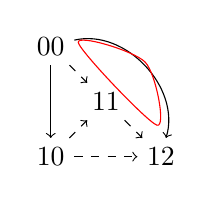
\begin{tikzpicture}
            \node (A) at (-0.7,0.7) {$00$};
            \node (B) at (-0.7,-0.7) {$10$};
            \node (C) at (0.7,-0.7) {$12$};
            \node (D) at (0,0) {$11$};
            \draw [-> ] (A) -- (B);
            \draw[->] (A) to [bend left=60] (C);
            \draw [->, dashed] (A) -- (D);
            \draw [->, dashed] (B) -- (C);
            \draw [->, dashed] (B) -- (D);
            \draw [->, dashed] (D) -- (C);
            \draw [red] [smooth cycle] plot coordinates { (-0.35,0.75) (0.65,-0.3) (0.5,0.5)};
        \end{tikzpicture}
    \ar[r]
    \ar[d, hook]
    &
        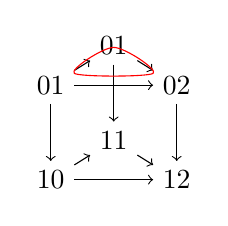
\begin{tikzpicture}
            \node (A) at (0, 0.85) {$01$};
            \node (B) at (-0.8, 0.35) {$01$};
            \node (C) at (0.8, 0.35) {$02$};
            \node (D) at (0, -0.35) {$11$};
            \node (E) at (-0.8, -0.85) {$10$};
            \node (F) at (0.8, -0.85) {$12$};
            \draw[->] (A) to (C);
            \draw[->] (A) to (D);
            \draw[->] (B) to (C);
            \draw[->] (B) to (A);
            \draw[->] (B) to (E);
            \draw[->] (C) to (F);
            \draw[->] (D) to (F);
            \draw[->] (E) to (F);
            \draw[->] (E) to (D);
            \draw [red] [smooth cycle] plot coordinates { (0,0.83) (0.5,0.5) (-0.5,0.5)};
        \end{tikzpicture}
    \ar[d, hook]
    \\
    \Delta^3
    \ar[r, hook, "h_0"']
    &
        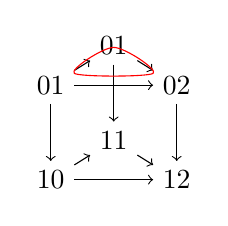
\begin{tikzpicture}
            \node (A) at (0, 0.85) {$01$};
            \node (B) at (-0.8, 0.35) {$01$};
            \node (C) at (0.8, 0.35) {$02$};
            \node (D) at (0, -0.35) {$11$};
            \node (E) at (-0.8, -0.85) {$10$};
            \node (F) at (0.8, -0.85) {$12$};
            \draw[->] (A) to (C);
            \draw[->] (A) to (D);
            \draw[->] (B) to (C);
            \draw[->] (B) to (A);
            \draw[->] (B) to (E);
            \draw[->] (C) to (F);
            \draw[->] (D) to (F);
            \draw[->] (E) to (F);
            \draw[->] (E) to (D);
            \draw [red] [smooth cycle] plot coordinates { (0,0.83) (0.5,0.5) (-0.5,0.5)};
        \end{tikzpicture}
    \end{tikzcd}
    \]
    
    For the case $(\overline{B}_1 \subseteq \overline{B}_2 = \overline{B}_3 )$ we exhibit each horn inclusion $\Lambda_k^n \hookrightarrow \Delta^n$ as a retract of a map in $\overline{B}_3$ for $0 \leq k \leq n$.
    \[
    \begin{tikzcd}
        \Lambda_k^n 
        \ar[r]
        \ar[d, hook]
        \ar[rr, bend left, "\id"]
        &
        (\Delta^1 \times \Lambda_k^n) \cup ( \Delta^{1} \times \Delta^1) 
        \ar[r]
        \ar[d, " \in B_3"]
        &
        \Lambda_k^n
        \ar[d]
        \\
        \Lambda^n 
        \ar[r]
        &
        \Delta^1 \times \Delta^n
        \ar[r]
        &
        \Delta^n
    \end{tikzcd}
    \]
    The vertical maps in the bottom row are given by the following composition of maps of partially ordered sets 
    \[
        [n] \xrightarrow{s} [1] \times [n] \xrightarrow{r} [n]    
    \]
    where the image of $s$ is given as follows
    \[
    s\colon
    \begin{tikzcd}
         01
        \ar[r]
        &
        02
        \ar[r]
        &
        \dotsc
        \ar[r]
        &
        0k
        \ar[rd]
        &
        \\
        &&&&
        1(k+1)
        \ar[r]
        &
        1(k+2)
        \ar[r]
        &
        \dotsc
        \ar[r]
        &
        1n
    \end{tikzcd}
    \]
    and the image of the map $r$ is given by
    \[
    r\colon
    \begin{tikzcd}
        0
        \ar[r]
        \ar[d]
        &
        1
        \ar[r]
        \ar[d]
        &
        2
        \ar[r]
        \ar[d]
        &
        \dotsc
        \ar[r]
        &
        k-1
        \ar[r]
        \ar[d]
        &
        k
        \ar[r]
        \ar[d]
        &
        \dotsc
        \ar[r]
        &
        k
        \ar[d]
        \\
        k
        \ar[r]
        &
        k
        \ar[r]
        &
        k
        \ar[r]
        &
        \dotsc
        \ar[r]
        &
        k
        \ar[r]
        &
        k+1
        \ar[r]
        &
        \dotsc
        \ar[r]
        &
        n
    \end{tikzcd}
    \]
\end{proof}

\begin{cor}
    Let $ S \xhookrightarrow{\iota} T$ be an anodyne extension and $L \xhookrightarrow{i}  K$ be an arbitrary inclusion.
    Then 
    \[
        (S \times K) \cup (T \times L) \xrightarrow{incl.} T \times K
    \]
    is an anodyne extension.
    In particular for $S= \Lambda_k^n$ and $T=\Delta^n$ we obtain that 
    \[
        (\Lambda_k^n \times K) \cup (\Delta^n \times L) \xrightarrow{incl.} \Delta^n \times K
    \]
    is an anodyne extension.
\end{cor}

\begin{proof}
    For 
    $ L \xrightarrow{i} K$ define $\mathcal{M} \coloneqq \{ S \xhookrightarrow{i} T \mid (S \times K) \cup (T \times L) \xrightarrow{} T \times K \text{ is anodyne}\}$
    Notice that $\mathcal{M}$ is a saturated class 
    hence if $\mathcal{M} \supseteq B_3 \implies \mathcal{M} = \overline{B}_3$.
    Consider $L' \hookrightarrow K'$ a monomorphism, that gives rise to $S = ( \Delta^1 \times L') \cup ( \Delta^{\{l\}} \times K') \to \Delta^1 \times K'= T$
    
    \[
    \begin{tikzcd}
        (((\Delta^1 \times L') \cup ( \Delta^{\{l\}} \times K')) \times K ) 
        \ar[r, " \in \An"]
        \ar[d, "\cong"]
        &
        (\Delta^1 \times K') \times K 
        \ar[d,"\cong"]
        \\
        \Delta^1 \times ( L' \times K \cup K' \times L) \cup ( \Delta^{\{l\}} \times (K' \times K) )
        \ar[r]
        &
        \Delta^1 \times (K' \times K)
    \end{tikzcd}
    \]
    Where the vertical map in the top row is in $B_3$ and thus an anodyne extension.
    It follows the bottom row is an anodyne extension as well, which we wanted to show.
\end{proof}

Let now $X$ be a Kan complex.

\begin{defi}
    Let $x \in X_0$ and $ n \geq 1$. We define 
    \[
    \pi_n(X,x) = \left\{ \Delta^n \xrightarrow{\alpha} X \mid 
    \begin{tikzcd}
        \partial
        \Delta^n
        \ar[r]
        \ar[d, hook]
        &
        \Delta^0
        \ar[d]
        \\
        \Delta^n
        \ar[r]
        &
        X
    \end{tikzcd}
    \right\}
    \big/ \text{htpy relative }\partial\Delta^n 
    \]
\end{defi}

\begin{defi}
\label{simplicial n-sphere}
    The (pointed) simplicial n-sphere is 
    \[
    \begin{tikzcd}
        \partial
        \Delta^n
        \ar[d]
        \ar[r, hook]
        &
        \Delta^n
        \ar[rdd, bend left, "\alpha"]
        \ar[d]
        \\
        \Delta^0
        \ar[r, "x"]
        \ar[drr, bend right, "x"']
        &
        \Delta^n/\partial \Delta^n = S^n
        \ar[rd, "\overline{\alpha}"]       
        \\
        &&
        X
    \end{tikzcd}
    \]
\end{defi}

\begin{prop}
    There are pullback squares $(\partial \Delta^n \xhookrightarrow{i} \Delta^n)$
    \[
    \begin{tikzcd}
        \underline{\Hom}(S^n,X)_x
        \ar[r]
        \ar[d]
        &
        \underline{\Hom}(S^n,X)
        \ar[d, "\ev_*"]
        \ar[r]
        &
        \underline{\Hom}(\Delta^n,X)
        \ar[d,"i^*"]
        \\
        \Delta^0
        \ar[r,"x"]
        \ar[rr, bend right ,"c(x)"']
        &
        X
        \cong 
        \underline{\Hom}(\Delta^0,X)
        \ar[r]
        &
        \underline{\Hom}(\partial \Delta^n,X)
    \end{tikzcd}
    \]
    where the vertical morphisms are Kan Fibrations and $\underline{\Hom}(S^n,X)_x$ is a Kan complex.
    Moreover the induced map 
    \[
        \underline{\Hom}(S^n,X)_x \to \underline{\Hom}(S^n,X)_{c(x)}
    \]
    is an isomorphism (between Kan complexes, since $X$ is a Kan complex).
\end{prop}

\begin{proof}
    Consider the following commutative square
    \[
    \begin{tikzcd}
        \Hom(\Delta^m \times S^n , X ) 
        \ar[r]
        \ar[d]
        &
        \Hom(\Delta^m \times \Delta^n , X )
        \ar[d]
        \\
        \Hom(\Delta^m \times \Delta^0 , X ) 
        \ar[r]
        &
        \Hom(\Delta^m \times \partial \Delta^n , X )
    \end{tikzcd}
    \] 
    this is a pullback since the Hom-functor sends colimits to limits and thus the diagram from \cref{simplicial n-sphere} to a pullback. 
    The left square is a pullback by construction and thus by the Pasting lemma 
    the outer square is a pullback as well.
\end{proof}

Lecture 12.11

\begin{prop}
    Let $X$ be a Kan complex and $x \in X_0$. Then the "old" and "new" definitions of $\pi_1(X,x)$ agree.
\end{prop}

\begin{proof}
    Consider the square
    \[
    \begin{tikzcd}
        \underline{\Hom}(\Delta^1, X)_{c(x)} 
        \ar[r]
        \ar[d]
        &
        \underline{\Hom}(\Delta^1, X)
        \ar[d, "i_*"]
        \\
        \Delta^0
        \ar[r, "{c(x)=(x,x)}"]
        &
        \underline{\Hom}(\partial \Delta^1, X) \cong X \times X
    \end{tikzcd}
    \]
    and let $f,g\colon \Delta^1 \to X$ such that $f_{\mid \partial \Delta^1}=(x,x)=g_{\mid \partial \Delta^1}$. 
    A homotopy $h\colon f \to g$ (rel $\partial \Delta^1$) is by definition 
    \[
    \begin{tikzcd}
        \Delta^{0}\times \Delta^{1}
        \ar[d]
        \ar[rd, bend left, "f"]
        &
        \\
        \Delta^1 \times \Delta^1
        \ar[r, "h"]
        &
        X
        \\
        \Delta^{1} \times \Delta^1
        \ar[u]
        \ar[ru, bend right, "g"']
    \end{tikzcd}
    \]
    the homotopy yields the following commutative square 
    \[
    \begin{tikzcd}
        x 
        \ar[r, "f"]
        \ar[d, equal]
        \ar[rd, "u"]
        &
        x
        \ar[d, equal]
        \\
        x
        \ar[r, "g"']
        &
        x
    \end{tikzcd}
    \]
\end{proof}

\underline{Aim}: To prove that $\pi_n(X,x)$ is a group for $n \geq 1$ (that is abelian for $n \geq 2$) as well as functoriality.
Fix $(X,x)$ where $X$ is a Kan complex $x \in X_0$, take n-simplices $\alpha, \beta  \colon  \Delta^n \to X$ representatives of classes in $\pi_n(X,x)$ that is $\alpha_{\mid \partial \Delta^n}= c(x) = \beta_{\mid \partial \Delta^n}$.
For $n=1$ this yields a horn, which can be extended since $X$ is a Kan complex. 
\[
\begin{tikzcd}
    &
    x
    \ar[rd, "\beta"]
    &
    \\
    x
    \ar[ru, "\alpha"]
    \ar[rr, dashed, "\gamma"']
    &&
    x
\end{tikzcd}
\]
For the general case we obtain a map from the horn (given on its n-simplices) as follows 
\[
\begin{tikzcd}
    \Lambda_n^{(n+1)}
    \ar[rr,"{(x,x,\dotsc,x,\alpha,\bullet,\beta)}"]
    \ar[d, hook]
    &&
    X
    \\
    \Delta^{(n+1)}
    \ar[rru, dashed, "\exists \sigma"']
    &&
\end{tikzcd}
\]
where $d_n\sigma\eqqcolon \gamma$ is the composition of $\alpha$ and $\beta$.
Now we define the multiplicative law on $\pi_n(X,x)$ by 
\begin{align*}
    \pi_n(X,x) \times \pi_n(X,x)& \to \pi_n(X,x)\\
    ([\alpha],[\beta])& \mapsto[\gamma]
\end{align*}

\begin{prop}
    The above binary operation is well defined.
\end{prop}

\begin{proof}
    We have $\alpha,\alpha',\beta,\beta'\colon \Delta^n \to X$ are representatives in $\pi_n(X,x)$ and
    \begin{align*}
        h_{n-1} \colon \Delta^1\times \Delta^n \to X \text{ htpy } \alpha \to \alpha' (\rel \partial \Delta^n)\\
        h_{n-1} \colon \Delta^1\times \Delta^n \to X \text{ htpy } \beta \to \beta' (\rel \partial \Delta^n)
    \end{align*}
    Choose $w,w' \colon \Delta^{n+1} \to X$ such that 
    \begin{align*}
        &\partial w = (x, \dotsc, x, \alpha, \gamma, \beta)\\
        &\partial w' = (x, \dotsc, x, \alpha', \gamma', \beta')
    \end{align*}
    Putting all this together we obtain 
    \[
    \begin{tikzcd}
        (\Delta^{(n+1)} \times \partial \Delta^1) \cup (\Delta^1 \times \Lambda_n^{n+1})
        \ar[rrr, "{(w,w',(x, \dotsc , x , h_{n-1}, \bullet, h_{n})}"]
        \ar[d, hook]
        &&&
        X
        \\
        \Delta^1 \times \Delta^{(n+1)}
        \ar[rrru, "w''"']
        &&
    \end{tikzcd}
    \]
    where $w''$ exists, since on the one summand we just have an inclusion and on the other we use that $X$ is a Kan complex.
    This way the composite
    \[
    h_n \colon \Delta^1 \times \Delta^n \xrightarrow{1 \times d^n} \Delta^1 \times \Delta^{n+1} \xrightarrow{w''} X
    \]
    is a homotopy from $\gamma$ to $\gamma'$ ($\rel \partial \Delta^n)$.
\end{proof}
Let us take a look at the case $n=1$ explicitely.
    
\[
    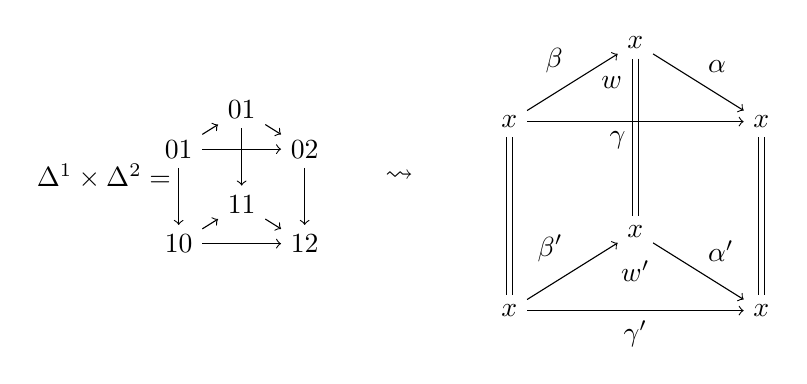
\begin{tikzpicture}
    \begin{scope}
        \node (0) at (-1.75,0) {$\Delta^1 \times \Delta^2 =$};
        \node (A) at (0, 0.85) {$01$};
        \node (B) at (-0.8, 0.35) {$01$};
        \node (C) at (0.8, 0.35) {$02$};
        \node (D) at (0, -0.35) {$11$};
        \node (E) at (-0.8, -0.85) {$10$};
        \node (F) at (0.8, -0.85) {$12$};
        \draw[->] (A) to (C);
        \draw[->] (A) to (D);
        \draw[->] (B) to (C);
        \draw[->] (B) to (A);
        \draw[->] (B) to (E);
        \draw[->] (C) to (F);
        \draw[->] (D) to (F);
        \draw[->] (E) to (F);
        \draw[->] (E) to (D);
    \end{scope}

    \begin{scope}[xshift=5cm]
        \node(arrow) at ( -3,0) {$\rightsquigarrow$};
        \node (A) at (0, 1.7) {$x$};
        \node (w) at (-0.3, 1.2) {$w$};
        \node (B) at (-1.6, 0.7) {$x$};
        \node (C) at (1.6, 0.7) {$x$};
        \node (D) at (0, -0.7) {$x$};
        \node (w') at (0, -1.2) {$w'$};
        \node (E) at (-1.6, -1.7) {$x$};
        \node (F) at (1.6, -1.7) {$x$};
        \draw[->] (A) to node[above right ]{$\alpha$} (C) ;
        \draw[double equal sign distance] (A) to (D) ;
        \draw[->] (B) to node[below left]{$\gamma$} (C);
        \draw[->] (B) to node[above left]{$\beta$} (A);
        \draw[double equal sign distance] (B) to (E) ;
        \draw[double equal sign distance] (C) to (F);
        \draw[->] (D) to node[above right ]{$\alpha'$} (F);
        \draw[->] (E) to node[below]{$\gamma'$} (F);
        \draw[->] (E) to node[above left]{$\beta'$} (D);
    \end{scope}
    \end{tikzpicture}
\]
\begin{prop}
    For all $n \geq 1$ it holds that $ \pi_n(X,x)$ is a group.
\end{prop}

\begin{proof}
    (Unitality) The neutral element in $\pi_n(X,x)$ is given by $[c(x)]$, where 
    \[
    c^n(x)\colon 
    \begin{tikzcd}
        &
        \Delta^0
        \ar[rd, "x"]
        &
        \\
        \Delta^n
        \ar[ru]
        \ar[rr]
        &&
        X
    \end{tikzcd}
    \]
    Let $w\coloneqq s_n(\alpha) \colon \Delta^{n+1} \to X$ for $\alpha\colon \Delta^n \to X$ such that $d_{n+1}(w)=d_{n+1}(s_n(\alpha))=\alpha=d_n(s_n(\alpha))=d_n(w)$.
    \[
    \begin{tikzcd}
        \Lambda_k^{n+1}
        \ar[d, hook]
        \ar[rrr, "{(x,x,\dotsc,x,c^n(x), \bullet, \alpha)}"]
        &&&
        X
        \\
        \Delta^{n+1}
        \ar[rrru, "w"']
    \end{tikzcd}
    \]
    where $[c^n(x)][\alpha]=[\alpha]$.

    (Associativity)
    Let $\alpha, \beta, \gamma \colon \Delta^n \to X$ be representatives of classes in $\pi_n(X,x)$.
    Choose $w_{n-1},w_{n+1},w_{n+2}\colon \Delta^{n+1} \to X$ such that 
    \begin{align*}
        \partial w_{n-1} =(x, \dotsc, x, \alpha, u, \beta) &; [\alpha][\beta]=[u]\\
        \partial w_{n+1} =(x, \dotsc, x, u, v, \gamma) &; [u][\gamma]=[v]\\
        \partial w_{n+2} =(x, \dotsc, x, \beta, \omega, \gamma) &; [\beta][\gamma]=[\omega]
    \end{align*}
    Let $q=(c^{n+1}(x), \dotsc , c^{n+1}(x), w_{n-1}, \bullet, w_{n+1}, w_{n+2})$, we obtain a diagram
    \[
    \begin{tikzcd}
        \Lambda_n^{n+2}
        \ar[r, "q"]
        \ar[d, hook]
        &
        X
        \\
        \Delta^{n+2}
        \ar[ru, " \exists \Tilde{w}"']
    \end{tikzcd}
    \]
    Now let us define $w_n \coloneqq d_n(\Tilde{w})$ and thus $\partial w_n = (x, \dotsc , x , \alpha, v, \omega) ; [\alpha][\omega]=[v]$. This results in 
    \[
    ([\alpha][\beta])[\gamma]=[u][\gamma]=[v]=[\alpha][w]=[\alpha]([\beta][\gamma])
    \]
    
    (Inverses)
    Let $\Delta^n \xrightarrow{\alpha} X$ be a representative of a calass in $\pi_n(X,x)$. 
    Consider the following horn-extension diagram
    \[
    \begin{tikzcd}
        \Lambda_n^{n+1}
        \ar[rrr, "{(x, \dotsc , x , \bullet , c^n(x), \alpha)}"]
        \arrow[d, hook]
        &&&
        X
        \\
        \Delta^{n+2}
        \ar[rrru, " \exists w"]
    \end{tikzcd}
    \]
    thus we get the equation $[d_{n-1}(w)][\alpha]=[c^n(x)]$

\underline{Aim}: Establish the functoriality of $\pi_n(X,x)$ and let $(X,x)$ and $(Y,y)$ be pairs such that $Y,X$ are Kan complexes $x \in X_0$ and $y \in Y_0$ and $f\colon X \to Y$ such that $f_0(x)=y$.
\[
    \begin{tikzcd}
        \underline{\Hom}(\Delta^n,X)_{c^n(x)}
        \ar[dd]
        \ar[rr]
        \ar[rd, "f_*"]
        &&
        \underline{\Hom}(\Delta^n,X)
        %\ar[d, "{\iota_*}"]
        \ar[rd, "f_*"]
        &
        \\
        &
        \underline{\Hom}(\Delta^n,Y)_{c^n(y)}
        \ar[dd]
        \ar[rr]
        &&
        \Hom(\Delta^n,Y)
        \ar[dd]
        \\
        \Delta^0
        \ar[rd, equal]
        \ar[rr, "c^n(x)"]
        &&
        \underline{\Hom(\partial \Delta^n,X)}
        \ar[rd, "f^*"]
        &
        \\
        &
        \Delta^0
        \ar[rr, "c^n(y)"]
        &&
        \underline{\Hom(\partial \Delta^n, X)}
    \end{tikzcd}
\]
For $i \colon \partial \Delta^n \to \Delta^n$.
Then $\pi_0(f_*) \eqqcolon \pi_n(f) \colon \pi_n(X,x) \to \pi_n(Y,y)$ is a morphism of pointed sets and gives the functoriality.
\end{proof}

\begin{defi}
    Let $\Delta^0/\SetD$ be the category of pointed sets.
\end{defi}

\begin{prop}
    Let $f\colon (X,x) \to (Y,y)$ be a morphism of pointed Kan complexes, then 
    \[
    \pi_n(f) \colon \pi_n(X,x) \to \pi_n(Y,y) 
    \]
    is a group homomorphism.
\end{prop}

\begin{proof}
    Let $\alpha, \beta \colon \Delta^n \to X$ be representatives of classes in $\pi_n(X,x)$ and
    $w \colon \Delta^{n+1} \to X$ where $\partial w = (x, \dotsc ,x , \alpha, \gamma , \beta)$ so that 
    $[\alpha][\beta]=[\gamma]$. But then
    \[
    f_*(w)\colon \Delta^{n+1}\xrightarrow{w}X \xrightarrow{f}Y
    \]
    has boundary $\partial (f_*(w))=(y, \dotsc , y, f_*(\alpha),f_*(\gamma),f_*(\beta))$
\end{proof}

\begin{prop}
    Let $f_1, f_2 \colon X \to Y$ and $g_1, g_2 \colon Y \to Z$ be morphisms between Kan complexes.
    Supose that $f_1 \sim f_2$ and $g_1 \sim g_2$, then $ g_1 \circ f_1 \sim g_2 \circ f_2$
\end{prop}

\begin{proof}
    Enough to treat the case $(f_1 = f_2, g_1 \sim g_2)$ and $(f_1 \sim f_2, g_1 = g_2)$.
    The first case is $f\coloneqq f_1 = f_2$ and $g_1 \sim g_2$, which gives 
    \[
    \begin{tikzcd}
        X  \cong \Delta^{\{0\}} \times X 
        \ar[r, "\id \times f"]
        \ar[d, "i_0 \times \id"']
        &
        \Delta^{\{0\}} \times Y
        \ar[d]
        \ar[rd, bend left, "g_1"]
        &
        \\
        \Delta^1 \times X
        \ar[r, "\id \times f"]
        &
        \Delta^1 \times X
        \ar[r, "h"]
        &
        Z
        \\
        X \cong \Delta^{\{1\}} \times X
        \ar[u, "i_1 \times \id"]
        \ar[r, "\id \times f"]
        &
        \Delta^{\{1\}}\times Y
        \ar[u]
        \ar[ru, bend right, "g_2"']
    \end{tikzcd}
    \]
    $h_f \colon g_1f \to g_2f$ is a homotopy of of the concatenation.

    The second case is $g\coloneqq g_1 = g_2$
    \[
    \begin{tikzcd}
        \Delta^{\{0\}}\times X
        \ar[d]
        \ar[dr, bend left, "f_1"]
        \ar[drr, bend left, "gf_1"]
        \\
        \Delta^1 \times X 
        \ar[r, "h"]
        &
        Y
        \ar[r]
        &
        Z
        \\
        \Delta^{\{1\}} \times X
        \ar[u]
        \ar[ru,bend right, "f_2"']
        \ar[rru,bend right, "gf_2"']
    \end{tikzcd}
    \]
    The horizontal composition then gives a homotopy from $gf_1$ to $gf_2$.
\end{proof}

\subsection{Exercises}

\begin{Exercise}
    
Consider a set $ G $ with two unital binary operations $ \otimes : G \times G \to G $.
Suppose that 
\[
    ( a \otimes b ) \cdot ( c \otimes d ) = ( a \cdot c ) \otimes ( b \cdot d )
\]
for all $ a , b, c , d \in G $.
\begin{enumerate}
    \item 
    Show that both units $e$ and $e_{\otimes}$ agree.

    \item 
    Deduce that $ \cdot = \otimes $.

    \item 
    Conclude that $ ( G , \cdot , e ) $ is an abelian monoid.
\end{enumerate}
\end{Exercise}


\begin{Exercise}
\label{Exercise_11.2}

Fix a Kan complex $ X $ and $ n \in \mathbb{N}_0$.

\begin{enumerate}[label=(\alph*)]
    \item 
    Let $ \alpha: \Delta^n \to X $ represent an element of $ \pi_n ( X , x ) $ for some $ x \in X_0 $ and $ n \in \mathbb{N}_0 $.
    Show that $ \alpha $ is homotopic to the neutral element $ x : \Delta^n \to \Delta^0 \xrightarrow{x} X $ if and only if there exists some $ \sigma \in \Delta^{n+1}$ such that $ d_i ( \sigma ) = x $ for $ 0 \leq  i \leq n $ and $ d_{n+1} ( \sigma ) = \alpha $.

    \item 
    Deduce that if $ p : X \to \Delta^0 $ is a trivial Kan fibration, i.e. $p \in r ( \{ \partial \Delta^n \to \Delta^n \mid n \in \mathbb{N}_0 \} )$, then $ \pi_n( X , x ) = 0 $ for all $ x \in X_0 $.

    \item 
    Deduce that for $X$ $n$-skeletal we have that $\pi_m ( X , x ) \cong 0 $ for any $ x \in X_0 $ and $ m \geq n $.

    \item 
    Show that for a group $ G $ we have that 
    \[
        \pi_n ( N ( BG ) , \star ) 
        \cong 
        \begin{cases}
            G &\text{ if }  n = 1
            \\
            0 &\text{ if }  n \neq 1
        \end{cases}
    \]
    where $ \star $ is the unique object of $ BG $.
\end{enumerate}
\end{Exercise}





% done

Lecture 17.12

\section{Trivial Kan fibrations, loop spaces and the Serre long exact sequence}

\underline{Construction}:
Let $X$ be a Kan complex and $x \in X_0$.
The \underline{(based) loop space} $\Omega(X,x)$ is given by the following pullback:
\[
\begin{tikzcd}
    \Omega(X,x)
    \ar[r]
    \ar[d]
    &
    \underline{\Hom(\Delta^1, X)}
    \ar[d, shift left=4, "i^*"]
    \ar[d, shift right=10]
    \\
    \Delta^0
    \ar[r, "{(x,x)}"]
    \ar[r, bend right, "c(x)"']
    &
    X\times X \cong \underline{\Hom(\partial \Delta^1 , X)}
\end{tikzcd}
\]
where $i^*$ is a Kan fibration and thus $\Omega(X,x)$ a Kan complex.
The \underline{path space} $\Pathspace X$ is given by the following diagram 
\[
\begin{tikzcd}
    \Omega(X,x) 
    \ar[d]
    \ar[r]
    &
    \Pathspace X
    \ar[r]
    \ar[d, "\pi"]
    &
    \underline{\Hom (\Delta^1,X)}
    \ar[d, "i^*"]
    \\
    \Delta^0
    \ar[rr, bend right, "{(x,x)}"']
    \ar[r]
    &
    X
    \ar[r,"{(i(x), \id_X)}"]
    &
    X \times X
    \cong 
    \underline{\Hom}(\partial \Delta^1, X)
\end{tikzcd}
\]

\underline{Aim}: Prove that for all $n \geq 0$ there is an isomorphism $\pi_{n+1}(X,x) \isomorphism \pi_n ( \Omega(X,x), 1_X)$ and that for all $n \geq 1$ the group $\pi_n(\Omega(X,x),1_X)$ is abelian and hence for all $n \geq 2$ the group $\pi_n(X,x)$ is abelian.
\begin{defi/prop}
\label{trivial_Kan_fibration}
    Let $p\colon X \to Y$ be a morphism in $\SetD$. The following are equivalent 
    \begin{enumerate}
        \item 
        $\{ \partial\Delta^n \hookrightarrow \Delta^n \mid n \geq 0 \} \lift{} p$
        \item 
        $\overline{\{ \partial\Delta^n \hookrightarrow \Delta^n \mid n  \geq 0\}} = \{\text{monomorphisms}\} \lift{} p$
    \end{enumerate}
    We call such a map a \underline{trivial Kan fibration}.
    Since $\Lambda_k^n \hookrightarrow \Delta^n$ is a monomorphism, all trivial Kan fibrations are especially Kan fibrations.
\end{defi/prop}

\begin{prop}
    Let $X \xrightarrow{p} \Delta^0$ be a trivial Kan fibration, then for all $x \in X$ and for all $n\geq 0$ the homotopy group is trivial, that is $\pi_n(X,x)=\{*\}$.
\end{prop}

\begin{proof}
    Exercise.    
\end{proof}

\begin{prop}
    Let $X \xrightarrow{p} Y$ be a Kan fibration and $L \xrightarrow{i}K$ be an anodyne extension, then
    $\underline{\Hom} (K,X) \to \underline{\Hom}(L,X) \times_{\underline{\Hom}(L,Y)} \underline{\Hom} (K,Y) $ is a trivial Kan fibration.    
\end{prop}

\begin{proof}
    The idea of the proof is the same as for 
    Exercise 10.4.
    \[
    \begin{tikzcd}
        (\Lambda_k^n \times L) \cup (\Delta^n \times K)
        \ar[r]
        \ar[d]
        &
        X
        \ar[d, "p"]
        \\
        \Delta^n \times L 
        \ar[r]
        \ar[ru, dashed, "\exists"]
        &
        Y
    \end{tikzcd}
    \]
    \[
    \begin{tikzcd}
        \partial \Delta^n 
        \ar[r]
        \ar[d]
        &
        \underline{\Hom}(K,X)
        \ar[d]
        \\
        \Delta^n 
        \ar[r]
        \ar[ru, dashed]
        &
        \underline{\Hom}(L,X) \times_{\underline{\Hom}(L,Y)} \underline{\Hom} (K,Y)
    \end{tikzcd}
    \]
\end{proof}

\begin{cor}
    Let $X$ be a Kan complex then there is a pullback square:
    \[
    \begin{tikzcd}
        \Pathspace X
        \ar[r]
        \ar[d, "p"]
        &
        \underline{\Hom}(\Delta^1,X)
        \ar[d, "i^*"]
        \\
        \Delta^0
        \ar[r, "x"]
        &
        \underline{\Hom}(\Delta^{\{0\}},X) \cong X
    \end{tikzcd}
    \]
    where $i^*$ is a trivial Kan fibration by \cref{trivial_Kan_fibration} and we claim that $p$ is one as well.
\end{cor}

\begin{proof}
    Consider the following diagram
    \[
    \begin{tikzcd}
        \Pathspace X 
        \ar[r]
        \ar[d, "\pi"']
        &
        \underline{\Hom(\Delta^1, X)}
        \ar[d]
        \ar[dd, bend left=90, "i^*"]
        \\
        X
        \ar[r, "{(c(x), \id_X)}"]
        \ar[d]
        &
        X \times X \cong \underline{\Hom ( \partial \Delta^1, X)}
        \ar[d, "\pi_0"]
        \\
        \Delta^0
        \ar[r, "x"]
        &
        X 
        \cong
        \underline{\Hom ( \Delta^{\{0\}}, X)}
    \end{tikzcd}
    \]
    We know the top square is a pullback, thus if the bottom one were one as well, then we would be done by the pasting lemma. So let us take a closer look here. 
    So the following diagram gives a pullback, where the first component of the map into the product is determined to be $c(x)$ by the commutativity of the square
    \[
    \begin{tikzcd}
        W 
        \ar[rdd, bend right]
        \ar[rrd, bend left, "{(f,g)=(c(x),g)}"]
        \ar[rd, dashed, "g"]
        &&
        \\
        &
        X
        \ar[r, "{(c(x), \id_X)}"]
        \ar[d]
        &
        X \times X
        \ar[d, "\pi_0"]
        \\
        &
        \Delta^0
        \ar[r]
        &
        X
    \end{tikzcd}
    \]
    \begin{cor}
        For all $x \in \Pathspace X_0$ and for all $n \geq 0$ we have that $\pi_n(\Pathspace X, x)= \{*\}$. 
    \end{cor}
    Let $X \xrightarrow{p} Y$ be a Kan fibration, with $X$ as well as $Y$ Kan complexes and $x \in X_0$ as well as $y=p(x) \in Y_0$. 
    Define
    \[
    \begin{tikzcd}
        F 
        \ar[r, "i"]
        \ar[d]
        &
        X
        \ar[d, "p"]
        \\
        \Delta^0 
        \ar[r, "y"]
        &
        Y
    \end{tikzcd}
    \]
    Notice that $x \in F_0$ by construction.
    By the functoriality of the homotopy groups we get a sequence 
    \[
    \pi_n(F,x)
    \xrightarrow{i_*}
    \pi_n(X,x)
    \xrightarrow{p_*}
    \pi_n(Y,y)
    \]
    for all $n \geq 0$.
\end{proof}

\begin{construction}
    Let $n \geq 1$ and $\alpha \colon \Delta^n \to Y$ be a representative of a class in $\pi_n(Y,y)$.
    Consider the following lifting diagram:
    \[
    \begin{tikzcd}
        \Lambda_0^n 
        \ar[d, hook]
        \ar[r]
        &
        \Delta^0
        \ar[r, "x"]
        &
        X
        \ar[d,"p"]
        \\
        \Delta^n
        \ar[rru, "\exists v"]
        \ar[rr,"\alpha"]
        &&
        Y
    \end{tikzcd}
    \]
    Where the left horn-inclusion is an anodyne extension and the morphism $p$ is a Kan fibration. Since Kan fibrations are exactly the morphisms with the right lifting property with respect to the anodyne extensions we get a lift $v$.
    We define $\partial ( [\alpha] ) = [d_0(v)]$ for $d_0(v)\colon \Delta^{n-1} \to F$, notice that since $F$ is a pullback there is a unique morphism into $F$ given by the morphism $d_0(v)$ that goes to $X$ and the unique morphism into the terminal object $\Delta^0$.
    So it makes sense to take $d_0(v)$ as a morphism into $F$.
    This defines a map $\partial \colon \pi_n(Y,y) \to \pi_n(F,x)$.

    We thus get a map $\partial \colon \pi_n(Y,y) \to \pi_{n-1}(F,x)$.
    To see this map is well defined consider $h\colon \Delta^1 \times \Delta^n \to Y$ a homtopy of $\alpha$ to $\alpha'$ ($\rel \partial \Delta^n$).
    Then we choose lifts 
    \[
    \begin{tikzcd}
        \Lambda_0^n
        \ar[r, "c(x)"]
        \ar[d, hook]
        &
        X
        \ar[d,"p"]
        \\
        \Delta^n 
        \ar[ru, dashed, "v"]
        \ar[r, "\alpha"]
        &
        Y
    \end{tikzcd}
    \qquad
    \begin{tikzcd}
        \Lambda_0^n
        \ar[r, "c(x)"]
        \ar[d, hook]
        &
        X
        \ar[d,"p"]
        \\
        \Delta^n 
        \ar[ru, dashed, "v'"]
        \ar[r, "\alpha'"]
        &
        Y
    \end{tikzcd}
    \]
    to obtain for the tuple $\omega=(v,v',(\bullet,x \dotsc, x))$ a lift
    \[
    \begin{tikzcd}
        (\partial \Lambda_k^n \times L) \cup (\Delta^n \times K)
        \ar[r, "\omega"]
        \ar[d, "\An \ni"']
        &
        X
        \ar[d, "p"]
        \\
        \Delta^n \times L 
        \ar[r]
        \ar[ru, dashed, "\exists \Tilde{h}"]
        &
        Y
    \end{tikzcd}
    \]
    which again exists since the left vertical map is anodyne and the morphism $p$ a Kan fibration.
    This results in 
    \[
        \Delta^1 \times \Delta^{n-1} \xrightarrow{\id \times d^0} \Delta^1 \times \Delta^n \xrightarrow{\Tilde{h}} X
    \]
    Now this is a homotopy of $d_0v$ to $d_0v'$ ($\rel \partial) \Delta^{n+1}$ and thus $[d_0v]=[d_0v']$.
    For $ n = 2 $ this amounts to the following picture.
    \[
    \begin{tikzcd}
        &
        01
        \ar[rd, "d_v"]
        \ar[dd, equal]
        \\
        00
        \ar[rr, equal]
        \ar[ru, equal]
        \ar[dd, equal]
        &&
        02
        \ar[dd, equal]
        \\
        &
        11
        \ar[rd, "d_0v'"]
        \\
        10
        \ar[ru, equal]
        \ar[rr, equal]
        &&
        12
    \end{tikzcd}
    \xrightarrow{p}
    \begin{tikzcd}
        &
        01
        \ar[rd, equal]
        \ar[dd, equal]
        \\
        00
        \ar[ru, equal]
        \ar[rr, equal]
        \ar[dd, equal]
        &&
        02
        \ar[dd, equal]
        \\
        &
        11
        \ar[rd, equal]
        \\
        10
        \ar[ru, equal]
        \ar[rr, equal]
        &&
        12
    \end{tikzcd}
    \]
\end{construction}

\begin{thm}{Serre's Long exact sequence}
\label{Serre's Long exact sequence}
    Let $X \xrightarrow{p} Y$ be a Kan fibration such that $Y$ is a Kan complex. Let $x \in X_0$ and $y\coloneqq p(x) \in Y_0$. Then there is a long exact sequence of pointed sets.
    \[
    \begin{tikzcd}
        & 
        \dotsc
        \rar
        \arrow[d, phantom, ""{coordinate, name=Z1}]
        &
        \pi_2(Y,y)
        \arrow[ dll,
                        "\partial", pos=1,
                        rounded corners,
                        to path={ -- ([xshift=2ex]\tikztostart.east)
                                  |- (Z1) \tikztonodes
                                  -| ([xshift=-2ex]\tikztotarget.west)
                                  -- (\tikztotarget)}
                      ]
        \\
        \pi_1(F,x)
        \rar
        & 
        \pi_1(X,x)
        \rar
        \arrow[d, phantom, ""{coordinate, name=Z}]
        &
        \pi_1(Y,y)
        \arrow[ dll,
                        "\partial", pos=1,
                        rounded corners,
                        to path={ -- ([xshift=2ex]\tikztostart.east)
                                  |- (Z) \tikztonodes
                                  -| ([xshift=-2ex]\tikztotarget.west)
                                  -- (\tikztotarget)}
                      ]
        \\
        \pi_0(F,x)
        \rar
        &
        \pi_0(X,x)
        \rar
        &
        \pi_0(Y,y)
    \end{tikzcd}
    \]
    for a given pullback square
    \[
    \begin{tikzcd}
        F
        \ar[r, "i"]
        \ar[d]
        &
        X
        \ar[d, "p"]
        \\
        \Delta^0
        \ar[r,"x"]
        &
        Y
    \end{tikzcd}
    \]
    We call a sequence of pointed sets $((A,a) \xrightarrow{f} (B,b) \xrightarrow{g} (C,c))$ exact if $\ker g \coloneqq \{b \in B \mid g(b) = c\} = \im (f)$. 
    Moreover there is a natural action of $\pi_1(Y,y)$ on $\pi_0(F,x)$ such that the stabilizer of $[x] \in \pi_1(Y,y)$ is precisely $\im(p_*)$, this means that $i_*([x'])=i_*([x''])$ if and only if $[x']$ and $[x'']$ are in some $\pi_1(Y,y)$-orbit.
\end{thm}

\begin{cor}
    Let $X$ be a Kan complex and $x \in X_0$. Take the pullback 
    \[
    \begin{tikzcd}
        \Omega(X,x)
        \rar
        \dar
        &
        \Pathspace X
        \ar[d, "\pi"]
        \\
        \Delta^0
        \rar
        &
        X
    \end{tikzcd}
    \]
    Then for all $n \geq 0$ the morphism $\pi_{n+1}(X,x) \xrightarrow{\partial} \pi_n(\Omega(X,x),1_x)$ is bijective.
\end{cor}

\begin{proof}
    By the Serre long exact sequence we have for all $n \geq 1$
    \[
    \{*\}=\pi_{n+1}(\Pathspace X,1_x) \to \pi_{n+1}(X,x) \xrightarrow[\sim]{\partial} \pi_n(F,x) \to \pi_n(\Pathspace X, 1_x)=\{*\}
    \]
    since $\partial$ is a group homomorphism here, we get the isomorphism.
    For $n=0$ we have
    \[
    \{*\}=\pi_{1}(\Pathspace X,1_x) \to \pi_{1}(X,x) \xrightarrow[\sim]{\partial} \pi_0(F,x) \to \pi_0(\Pathspace X, 1_x)=\{*\}
    \]
    notice that $\pi_0(F,1_x)$ and $\pi_(\Pathspace X,1_x)$ are not groups, thus we need to use the orbit stabilizer theorem and the last part of \cref{Serre's Long exact sequence} to obtain that $\partial$ is a bijection.
\end{proof}

\begin{prop}
    The map $\partial\colon \pi_n(Y,y) \to \pi_{n-1}(F,x)$ is a group homomorphism for $n \geq 2$.
\end{prop}

\begin{proof}
    Let $\omega \colon \Delta^{n+1} \to Y$ be an (n+1)-simplex, such that
    $\partial \omega = ( y, \dotsc , y , \alpha_{n-1}, \alpha_n , \alpha_{n+1})$. Furthermore $\omega$ is a witness of $[\alpha_{n-1}][\alpha_{n+1}]=[\alpha_n]$ in $\pi_n(Y,y)$.
    Choose (for $i=n-1,n,n+1)$ witnesses of $\partial([\alpha_i])=[d_0v_i]$
    \[
    \begin{tikzcd}
        \Lambda_0^n
        \ar[r, "c(x)"]
        \ar[d]
        &
        X
        \ar[d, "p"]
        \\
        \Delta^n
        \ar[ru, dashed, "v_i"]
        \ar[r, "\alpha_i"']
        &
        Y
    \end{tikzcd}
    \]
    \[
    \begin{tikzcd}
        \Lambda^{n+1}_0
        \ar[rrr, "{(x,\dotsc,x, v_{n-1},v_n,v_{n+1})}"]
        \dar
        &&&
        X
        \dar["p"]
        \\
        \Delta^{n+1}
        \ar[rrru, dashed, "\exists \gamma"]
        \ar[rrr, "\omega"']
        &&&
        Y
    \end{tikzcd}
    \]
    We get the folowing equation $\partial([\alpha_{n-1}]) \partial([\alpha_{n+1}])=[d_0v_{n-1}][d_0v_{n+1}]=[d_0v_n]=\partial([\alpha_n])=\partial([\alpha_{n-1}][\alpha_{n+1}])$.
    Then $d_0\gamma$ is a witness of the above composition since $\partial(d_0\gamma)=(x,\dotsc,x, d_0v_{n-1}, d_0v_n, d_0v_{n+1})$.
    We now want to show (parts of) the exactness of Serre's long exact sequence.
    Let
    \[
        [\alpha] \in \pi_n(F,x) \xrightarrow{i_*} \pi_n(X,x) \xrightarrow{p_*}
        \pi_n(Y,y)
    \]
    be the sequence of homtopygroups.
    Then we have the following square
    \[
    \begin{tikzcd}
        \Delta^n
        \ar[r, "\alpha"]
        \ar[d]
        &
        X
        \ar[d, "p"]
        \\
        \Delta^0
        \ar[r,"y"]
        &
        Y
    \end{tikzcd}
    \]
    This shows that $ \im(i_*) \subseteq \ker(p_*)$.
    Conversely, if we have a commutative diagram
    \[
    \begin{tikzcd}
        \Delta^n
        \ar[r, "\alpha"]
        \ar[d]
        \ar[rd, "p_*\alpha"]
        &
        X
        \ar[d, "p"]
        \\
        \Delta^0
        \ar[r,"y"]
        &
        Y
    \end{tikzcd}
    \]
    Then $\alpha \colon \Delta^n \to  X$ is an $n$-simplex of the fibre
    $\pi_n(X,x) \xrightarrow{p_*} \pi_n(Y,y) \xrightarrow{\partial} \pi_{n-1}(F,x)$.
    To show $\im(p_*) \subseteq  \ker(\partial)$, take an $n$-simplex and extend it along $p$
    \[
    \begin{tikzcd}
        \Delta^n
        \ar[r,"\alpha"]
        \ar[rd, "p_{\alpha}"']
        &
        X
        \ar[d,"p"]
        \\
        &
        Y
    \end{tikzcd}
    \]
    This can be completed to a commutative square 
    \[
        \begin{tikzcd}
        \Lambda_0^n
        \dar
        \ar[r,"c(x)"]
        &
        X
        \ar[d,"p"]
        \\
        \Delta^n
        \ar[ru, "\alpha"]
        \ar[r, "p_{\alpha}"]
        &
        Y
        \end{tikzcd}
    \]
    where $\partial[p_*\alpha]=[d_0\alpha]=c(x)$.
    To show that $\im(p_*) \supseteq \ker \partial$, let $[\alpha] \in \pi_n(Y,y)$ such that $\partial([\alpha])=[d_0v]=[c(x)]$, that is $[\alpha] \in \ker \partial$.
    This means we have a homotopy from $[d_0v]$ to $[c(x)]$
    \[
    \begin{tikzcd}
        \Delta^{\{0\}} \times \Delta^{n-1}
        \ar[d, hook]
        \ar[dr, bend left, "d_0v"]
        &
        \\
        \Delta^1 \times \Delta^{n-1}
        \ar[r, "\exists h_0"]
        &
        X
        \\
        \Delta^{\{1\}} \times \Delta^n
        \ar[u, hook]
        \ar[ru, bend right, "c(x)"']
    \end{tikzcd}
    \]
    We thus obtain a commutative square
    \[
    \begin{tikzcd}
        &
        (\Delta^{\{1\}} \times \Delta^n) \cup ( \Delta^1 \times \partial \Delta^n)
        \ar[rrr, "{(v ( h_0, x , \dotsc , x ))}"]
        \ar[d, hook]
        &&&
        X
        \ar[d, "p"]
        \\
        \Delta^{\{1\}} \times \Delta^n
        \ar[r]
        &
        \Delta^1 \times \Delta^n
        \ar[rrru, "\exists \Tilde{h}"]
        \ar[rrr, "h\coloneqq p \Tilde{h}"]
        &&&
        Y
    \end{tikzcd}
    \]
    Then $h$ is a homotopy $\alpha \to p( \Tilde{h}d^1)$ $\rel \partial\Delta^n$
    The rest of the proof is given as exercise.
\end{proof}

\subsection{Interlude}

As we know, $\Kan \subseteq \SetD $ and we can pass to $\hKan$ the homotopy category of Kan complexes. 
Since we wish to interpret Kan complexes as models for $\infty$-groupoids, we have been studying "the homotopy category of $\infty$-groupoids."

\subsection{Challenge}

We wish to regard homotopy equivalent Kan complexes as being isomorphic, while having access to universal properties (limit/colimit constructions).

\underline{Aim}: Understand how to use $\SetD$ to study the $(\infty,1)$-category of Kan complexes in which instead of Hom sets we have "Hom Kan complexes" (="Hom $\infty$-groupoids").

\begin{defi}
    Let $X \xrightarrow{f} Y$ be a map of Kan complexes. Then $f$ is a \underline{weak homotopy equivalence} if $\forall x \in X$ and $\forall n \geq 0$, $\pi_n(f) \colon  \pi_n(X,x) \isomorphism \pi_n(Y,f(x))$.
\end{defi}

\begin{rmk}
    By Whitehead's theorem for a category $\mathcal{C}$ and $W \subseteq \Mor (\mathcal{C})$ a class of maps, we obtain:
    \[
    \begin{tikzcd}
        \SetD
        \rar
        \ar[rd]
        &
        \Gpd_{\infty}= \SetD[Weq^{-1}]_{(\infty, 1) cat}
        \ar[d]
        \\
        &
        \hKan
    \end{tikzcd}
    \]
\end{rmk}

We are not gonna detail the motivation here, since it is going to be extended in its formality in the nexte lectures.

\begin{cor}
    Let $X \xrightarrow{p} Y$ be a Kan fibration and $f\colon y_0 \to y_1$ be an edge in $Y$.
    Then there exist $X_{y_0} \xleftarrow{} \bullet \to X_{y_1}$ trivial Kan fibrations.
\end{cor}

\begin{proof}
    For 
    \[
    \begin{tikzcd}
        W
        \ar[r,"q"]
        \ar[d, "r"']
        &
        Y
        \\
        X
        \ar[ru, "p"']
    \end{tikzcd}
    \]
    define $\underline{\Hom}_Y((W,q)(X,p))$ by and take the pullback
    \[
    \begin{tikzcd}
        \underline{\Hom_Y}((W,q),(X,p)) 
        \ar[d]
        \rar
        &
        \underline{\Hom}(W,X)
        \ar[d, "p_*"]
        \\
        \Delta^0
        \ar[r, "q"]
        &
        \underline{\Hom}(W,Y)
    \end{tikzcd}
    \]
    Where both vertical maps are Kan fibrations.
    Consider for example a morphism from the trivial simplicial set $\Delta^0 \xrightarrow{y_e}Y$ then
    \[
    \begin{tikzcd}
        X_{y_e}=\underline{\Hom}_Y((\Delta^0,y_e)(X,\circ)) 
        \rar
        \dar
        &
        \underline{\Hom}(\Delta^0,X)
        \ar[r,"\sim"]
        \ar[d, "p_*"]
        &
        X
        \ar[d,"p"]
        \\
        \Delta^0
        \ar[r,"y_e"]
        &
        \underline{\Hom}(\Delta^0,Y)
        \ar[r, "\sim"]
        &
        Y
    \end{tikzcd}
    \]
    Consider now the pullback-square 
    \[
        \begin{tikzcd}
            \underline{\Hom}_Y((\Delta^1,f),(X,p))
            \rar
            \dar
            &
            \underline{\Hom}(\Delta^1,X)
            \dar
            \\
            \underline{\Hom}_Y((\Delta^{\{l\}},y_e),(X,p))
            \ar[r]
            &
            \underline{\Hom}(\Delta^1,Y) \times_{\underline{\Hom}}(\Delta^{\{l\}},Y) \underline{\Hom}(\Delta^{\{l\}},X)
        \end{tikzcd}
    \]
\end{proof}

Lecture 7.1

\begin{prop}
    Let $X$ be a Kan complex. 
    Then $\pi_1(\Omega(X,x),1_X)$ is abelian.
\end{prop}

\begin{proof}
    We have $\pi_1(\Omega(X,x),1_X)$ has 2 binary operations.
    By the Eckmann Hilton argument the result follows.
    The details of that are to be worked out in the exercises.

Let now $\alpha\colon \Delta^1 \to \Omega(X,x) $ be a 1-simplex of the loop space.
Take the pullback diagram:
\[
\begin{tikzcd}
    \Delta^1
    \ar[rd,"\alpha"]
    \ar[rrd, bend left]
    \ar[rdd, bend right]
    &&
    \\
    &
    \Omega(X,x)
    \rar
    \dar
    &
    \underline{\Hom}(\Delta^1,X)
    \ar[d, "{(s,t)}"]
    \\
    &
    \Delta^0
    \ar[r, "{(X,x)}"]
    &
    X \times X \cong \underline{\Hom}(\partial \Delta^1, X)
\end{tikzcd}
\]

\[
    \begin{tikzcd}
        x
        \ar[d,"1_x"']
        \ar[r,"1_x"]
        &
        x
        \ar[d,"1_x"]
        \\
        x
        \ar[r,"1_x"']
        &
        x
    \end{tikzcd}
\]

We see that binary operations correspond to "vertical stacking" and "horizontal stacking".
\[
\begin{tikzcd}
    x
    \ar[r]
    \ar[d]
    \ar[r, phantom, shift right =3.4ex, "\beta" ]
    \ar[rr, bend left]
    \ar[dd, bend right]
    &
    x
    \ar[r]
    \ar[d]
    \ar[r, phantom, shift right =3.4ex, "\partial" ]
    &
    x
    \dar
    \ar[dd, bend left]
    \\
    x
    \ar[r]
    \ar[d]
    \ar[r, phantom, shift right =3.4ex, "\alpha" ]
    \ar[rr, bend left]
    &
    x
    \ar[r]
    \ar[d]
    \ar[r, phantom, shift right =3.4ex, "\gamma" ]
    &
    x
    \dar
    \\
    x
    \rar
    \ar[rr,bend right]
    &
    x
    \rar
    &
    x
\end{tikzcd}
\begin{tikzcd}[column sep=4ex,row sep=1ex, ampersand replacement=\&]
    \ar[r, "{\begin{pmatrix}
        \beta  & \partial \\
        \alpha & \gamma
        \end{pmatrix}}"]
    \&
    X
    \&
    \\
    \ar[r, hook, "{\in \An}"']
    \&
    (\Lambda_1^2 \times \Delta^2) \cup ( \Delta^2 \times \Lambda_1^2)
    \ar[r, hook, "{\in \An}"']
    \&
    \Delta^2 \times \Delta^2
    \ar[lu, "w"']
\end{tikzcd}
\]


    $([\alpha] \circ [\beta]) \bullet ( [\gamma] \circ [\partial])$
    
     $=( \left[
    \begin{tikzcd}
        00
        \rar
        \dar
        &
        01
        \dar
        \\
        10
        \rar
        &
        21
    \end{tikzcd}
    \right] ) 
    \circ ( \left[ 
    \begin{tikzcd}
        01
        \rar
        \dar
        &
        02
        \dar
        \\
        21 
        \rar
        &
        22
    \end{tikzcd}
    \right] )
    =
    ( \left[
    \begin{tikzcd}
        00
        \rar
        \dar
        &
        02
        \dar
        \\
        20
        \rar
        &
        22
    \end{tikzcd}
    \right] )$ 

    
    $=
    ( \left[
    \begin{tikzcd}
        10
        \rar
        \dar
        &
        12
        \dar
        \\
        20
        \rar
        &
        22
    \end{tikzcd}
    \right] ) \circ
    ( \left[
    \begin{tikzcd}
        00
        \rar
        \dar
        &
        02
        \dar
        \\
        10
        \rar
        &
        12
    \end{tikzcd}
    \right] ) 
$
\end{proof}

\subsection{Exercises}

\begin{Exercise}
    
Let $p: X  \to Y$ be a Kan fibration with $ Y $ a Kan complex. 
Recall that for $ x \in X_0 $ we may construct the fibre $ F $ of $ p $ at $ p ( x ) $ via the following pullback diagram.
\[
\begin{tikzcd}
    F 
    \ar[r, "i"]
    \dar
    &
    X
    \ar[d,"p"]
    \\
    \Delta^0
    \ar[r,"p(x)"]
    &
    Y
\end{tikzcd}
\]

\begin{enumerate}
    \item 
    Show that both $ F $ and $ X $ are Kan complexes and that $ x $ may be naturally be viewed as an object $ F $.
    
\end{enumerate}

In the lecture we have constructed a morphism $ \partial : \pi_{n+1} ( Y , p ( x ) ) \to \pi_n ( F , x ) $ which assigns to $\alpha : \Delta^{ n + 1 } \to Y $ the 0th face of $ \theta $ where $ \theta $ is a solution to the 0-horn lifting problem induced by $ \alpha $ and the constant map $ x : \Lambda_0^{n+1} \to \Delta^0 \to X $ for each $ n \in \mathbb{N}_0$.
Furthermore, we have established in the lecture that $\partial$ is a group homomorphism for $ n \in \mathbb{N}_+ $.
Our goal in this exercise is to show that the ensuing long sequence
\[
    \dotsc 
    \xrightarrow{\partial}
    \pi_1 ( F , x ) 
    \xrightarrow{\pi_1(i)}
    \pi_1 ( X , x )
    \xrightarrow{\pi_1 ( p )}
    \pi_1 ( Y , p ( x ) )
    \xrightarrow{\partial}
    \pi_0 ( F , x ) 
    \xrightarrow{\pi_0(i)}
    \pi_0(X,x)
    \xrightarrow{\pi_0(p)}
    \pi_0(Y,p(x))
\]
is in fact a long exact sequence of groups respective pointed sets.
(Recall that a group is canonically a pointed set by taking the neutral element as base point and that the kernel of a morphism of pointed sets is defined as the preimage of the distinguished element.) 
To this end, we have shown already in the lecture that 
\[
    \pi_n( F , x ) 
    \xrightarrow{\pi_n(i)}
    \pi_n ( X ,x ) 
    \xrightarrow{\pi_n ( p )}
    \pi_n( Y , p ( x )  )
\]
are exact segments for all $ n \in \mathbb{ N }_0 $ and that the segments
\[
    \pi_{n+1}( X , x )
    \xrightarrow{\pi_{n+1}(p)}
    \pi_{n+1} ( Y , p ( x ) ) 
    \xrightarrow{ \partial }
    \pi_n ( F , x )
\]
are exact for $ n \in \mathbb{N}_+ $

\begin{enumerate}[label=(\alph*), resume]
    \item 
    Show that the segment 
    \[
        \pi_{n+1} ( Y , p ( x ) ) 
        \xrightarrow{ \partial }
        \pi_n ( F , x )
        \xrightarrow{ \pi_n ( i ) }
        \pi_n ( X , x ) 
    \]
    is exact for every $ n \in \mathbb{ N }_+ $, i.e. $\im ( \partial ) = \ker ( \pi_n ( i ) ) $.
\end{enumerate}

For $ y \in F_0 $ we obtain a lifting problem
\[
\begin{tikzcd}
    \Lambda_0^1
    \ar[r, "v"]
    \ar[d]
    &
    X
    \ar[d, "p"]
    \\
    \Delta^1 
    \ar[ru, dashed, " \exists \theta "]
    \ar[r, " \alpha "]
    &
    Y
\end{tikzcd}
\]
for any $ \alpha $ representing a class of $ \pi_1 ( Y , p ( x ) ) $.
Let $ \theta $ be a solution to this lifting problem and define $ [ \alpha ] \cdot [ v ] \coloneqq [ d_0 ( \theta ) ]$.

\begin{enumerate}[label=(\alph*), resume]
    \item 
    Argue that the above is a well defined action of $ \pi_1 ( Y , p ( x ) ) $ on $ \pi_0 ( F ,x ) $ and describe $ \partial $ in terms of the action for $ n = 0 $.

    \item 
    Show that $ [ \alpha ] \cdot [ x ] = [ x ] $ for $ [ \alpha ] \in \pi_1( Y , p ( x ) ) $ if and only if $ [ \alpha ] \in \im ( \pi_1 ( p ) )$, i.e. that the image of $ \pi_1(p) $ is the stabilizer of the distinguished point $ [ x ] $. In other words, the segment 
    \[
        \pi_1( X , x ) 
        \xrightarrow{\pi_1 ( p )}
        \pi_1 ( Y , p ( x ) ) 
        \xrightarrow{ \partial }
        \pi_0 ( F , x ) 
    \]
    is exact.

    \item 
    Show that $ \pi_0 ( i ) ( [v] ) = \pi_0 ( i ) ( [ w ] ) $ if and only if there exists some $ [ a ] \in \pi_1 ( Y , p ( x ) ) $ such that $ [ \alpha ] \cdot [ v ] = [ w ] $. 
    Deduce from this the exactness for $ n = 0 $ in (b).

    \item 
    Finally, conclude from Exercise 11.2 that, if $ p : X \to Y $ is a trivial Kan fibration, then $ p $ is a weak homotopy equivalence, i.e. $ \pi_n ( p ) = \pi_n ( p ,x )$ is an isomorphism for all $ n \in \mathbb{N}_0 $ and $ x \in X_0 $.
\end{enumerate}

We will show later that a Kan fibration which is a weak homotopy equivalence is itself a trivial Kan fibration.
\end{Exercise}

    

\begin{Exercise}
Recall from Exercise 10.1 the class of trivial Kan fibrations, $ r ( \text{ Monomorphsisms } ) $.

\begin{enumerate}[label=(\alph*)]
    \item 
    Show that any trivial Kan fibration $ p \colon X \to Y $ admits a section $ s \colon Y \to X $ such that $ p \circ s = \id_Y $.
    
\end{enumerate}

A morphism $ s \colon Y \to X $ of simplicial sets is a deformation retract if there exists a retraction $ r \colon X \to Y $ with $ r \circ s = \id_Y $ and a homotopy $ h \colon \Delta^1 \times X \to X $ such that $ \partial_0 ( h ) = \id_X $ and $ \partial_1 ( h ) = s \circ r $.
Here we write $ \partial_{ \epsilon} = ( \{ \epsilon \} \times \id_Y )^*$ for $ \epsilon \in \Delta^1_0 $.
We say that $ s $ is a strong deformation retract if we have additionally that $ h \circ  ( \id_{ \Delta^1 } \times s ) = ( s_0)_* \times s $

\begin{enumerate}[label=(\alph*), resume]
    \item 
    Show that any section of a trivial Kan fibration is in fact a strong deformation retract.

    \item 
    Deduce that a trivial Kan fibration is a homotopy equivalence, i.e. invertible up to homotopy.
\end{enumerate}
\end{Exercise}


 %done

\section{Quillens small object argument}

Let $\mathcal{C}$ be a category that has all small colimits, let furthermore $\mathcal{C}$ be a cocomplete category (e.g. $\SetD$)
and $J$ a set of morphisms in $\mathcal{C}$

\underline{Aim}: For all $f$ in $\mathcal{C}$ construct a factorisation under some assumption in $J$.
\[
\begin{tikzcd}
    &
    \bullet
    \ar[rd, "{\in J^{\lift{}}}"]
    &
    \\
    \bullet
    \ar[ru, " \prescript{\lift{}}{}{(J^{\lift{}})} \ni"]
    \ar[rr, "f"']
    &&
    \bullet
\end{tikzcd}
\]

That is $J= \{ \Lambda_k^n \xhookrightarrow{} \Delta^n \mid n\geq 1, 0 \leq k \leq n\}$ and then $J^{\lift{}}=$Kan fibrations, or $J=\{ \partial \Delta^n \hookrightarrow \Delta^n \mid n \geq 0 \}$ and then $J^{\lift{}}=$Trivial Kan fibrations.
But we also want this factorisation to be functorial.

\begin{defi}
    A functorial factorisation in $\mathcal{C}$ is a section
    $\Fun([1], \mathcal{C}) \to \Fun([2], \mathcal{C})$
    of the composition functor $\Fun([2], \mathcal{C}) \xrightarrow{? \circ d_1}\Fun([1], \mathcal{C})$
    where $([1] \xrightarrow{d_1} [2] \to \mathcal{C})$.
\end{defi}

Let us unravel the definition:
For all morphisms $x \xrightarrow{f}y$ in $\mathcal{C}$ we get a $2$-simplex
\[
    \begin{tikzcd}
        &
        U(f) \ar[rd,"Rf"]
        &
        \\
        x
        \ar[ru, "Lf"]
        \ar[rr, "f"']
        &&
        y
    \end{tikzcd}
\]
in $\mathcal{C}$.
For all commutative squares 
\[
\begin{tikzcd}
    x
    \ar[r, "f"]
    \ar[d, "a"']
    &
    y
    \ar[d, "b"]
    \\
    x'
    \ar[r, "f'"']
    &
    y'
\end{tikzcd}
\]
in $\mathcal{C}$, we get a diagram
\[
\begin{tikzcd}
    &
    U(f)
    \ar[dd, dashed, "{U(a,b)}" pos=0.7]
    \ar[dr,"R(f)"]
    \\
    x
    \ar[dd,"a"']
    \ar[rr,"f" pos=0.3]
    \ar[ru,"Lf"]
    &&
    y
    \ar[dd,"b"]
    \\
    &
    U(f')
    \ar[rd,"Rf'"]
    \\
    x'
    \ar[ru,"Lf'"]
    \ar[rr,"f'"']
    &&
    y'
\end{tikzcd}
\]

\begin{defi}
\label{weak factorisation system}
    A weak factorisation system $(\mathcal{L},\mathcal{R})$ in $\mathcal{C}$ is a pair of classes of morphisms such that the following properties hold:
    \begin{enumerate}
        \item 
        (Factorisation) For all morphism $f:x\to y$ in $\mathcal{C}$ there exists a $2$-simplex
        \[
        \begin{tikzcd}
            &
            z
            \ar[rd,"\in \mathcal{R}"]
            \\
            x
            \ar[ru, " \mathcal{L} \ni"]
            \ar[rr, "f"']
            &&
            y
        \end{tikzcd}
        \],
        \item 
        (Lifting) $\mathcal{L} \lift{} \mathcal{R}$,
        \item 
        (Closure) $\mathcal{L} = \prescript{\lift{}}{}{\mathcal{R}}$ and $\mathcal{L}^{\lift{}} = \mathcal{R}$.
    \end{enumerate}
\end{defi}

\begin{lem}{The retract argument}
Suppose 
$
\begin{tikzcd}
    \bullet
    \ar[d, "f"]
    \ar[r, "l"]
    &
    \bullet
    \ar[d, "r"]
    \\
    \bullet 
    \ar[r, equal]
    &
    \bullet
\end{tikzcd}
$
and $f \lift{} r$. Then $f$ is a retract of $l$ as objects in the arrow category .
\end{lem}

\begin{proof}
Since $f$ has the left lifting property with respect to $r$, we get a lift
    \begin{tikzcd}
        \bullet
        \ar[d, "f"]
        \ar[r, "l"]
        &
        \bullet
        \ar[d, "r"]
        \\
        \bullet 
        \ar[ru, "w"]
        \ar[r, equal]
        &
        \bullet
    \end{tikzcd}
We can rewrite this diagram:
\[
    \begin{tikzcd}
        \bullet 
        \ar[r, equal]
        \ar[d, "f"]
        &
        \bullet
        \ar[r, equal]
        \ar[d, "l"]
        &
        \bullet
        \ar[d, "f"']
        \\
        \bullet
        \ar[rr, bend right, "\id"]
        \ar[r, dashed, "w"']
        &
        \bullet
        \ar[r, "r"]
        &
        \bullet
    \end{tikzcd}
\]
\end{proof}

\begin{lem}
    Suppose $(\mathcal{L}, \mathcal{R})$ satisfy the properties Factorisation and Lifting from \cref{weak factorisation system}.
    Then the property Closure holds if and only if $\mathcal{L}, \mathcal{R}$ are closed under retracts.
\end{lem}

\begin{proof}
    \todo{I am not convinced here, are we using the wrong idea of retract here?}
\end{proof}

\begin{thm}{Quillen's small object argument}
\label{Quillen's small object argument}
    Let $\mathcal{C}$ be a cocomplete category, $J$ a set of morphisms in $\mathcal{C}$ suppose that for all $j \in J$ we have that $\Hom_{\mathcal{C}}(\dom j,-)\colon \mathcal{C} \to \Set$ preserve (countable) sequential colimits (shape $(\mathcal{N}, \leq )$.
    Then there exists a functorial factorisation in $\mathcal{C}$ turning $(\prescript{\lift{}}{}{(J^{\lift{}})},J^{\lift{}})$ into a weak factorisation system.
    Moreover $\prescript{\lift{}}{}{(J^{\lift{}})}$ is the saturation of $J$.
\end{thm}

\begin{proof}
    Let $f$ be a morphism in $\mathcal{C}$.
    For $j \in J$, let $S_q(j,f)=
    \left\{ 
        \begin{tikzcd}
        \bullet
        \ar[d, "i"]
        \ar[r]
        &
        \bullet
        \ar[d, "f"]
        \\
        \bullet 
        \ar[r]
        &
        \bullet
        \end{tikzcd}
    \right\}$
    \[
    \coprod_{j\in J}\coprod_{S_q(j,f)}
    \begin{tikzcd}
        \bullet
        \ar[d, "j"]
        \ar[r, "d_f"]
        &
        \bullet
        \ar[d, "f"]
        \\
        \bullet 
        \ar[r, "c_f"']
        &
        \bullet
    \end{tikzcd}
    \]
    Consider now the pushout:
    \[
    \coprod_{j\in J}\coprod_{S_q(j,f)}
    \begin{tikzcd}
        \bullet
        \ar[r, "d_f"]
        \ar[d]
        \ar[r, phantom, shift right =3.4ex, "\PO" ]
        &
        \bullet
        \ar[d, "Lf"]
        \ar[r, equal]
        &
        \bullet
        \ar[d, "f"]
        \\
        \bullet
        \ar[r,"b_f"']
        &
        x_1 
        \ar[r, "Rf"']
        &
        \bullet
    \end{tikzcd}
    \]
    By construction $Lf \in \prescript{\lift{}}{}{(J^{\lift{}})}$, but we have no guarantee that $Rf \in J^{\lift{}}$.
    Apply now the above construction to $Rf$ and thus we obtain a square:
    \[
    \begin{tikzcd}
        x_1 
        \ar[r, equal]
        \ar[d, "LRf"]
        &
        x_1
        \ar[d, "Rf"]
        \\
        x_2
        \ar[r, "R^2f"]
        &
        x_2
    \end{tikzcd}
    \]
    Repeating the construction iteratively we obtain a diagram:
    \[
    \begin{tikzcd}
        x_0
        \ar[r, "Lf"]
        \ar[rrd, bend right, "f"]
        \ar[rrrrr, bend left, "{L^wf \in \prescript{\lift{}}{}{(J^{\lift{}})}}" ]
        &
        x_1
        \ar[r,"LRf"]
        \ar[rd, bend right, "Rf"]
        &
        x_2
        \ar[r, "LR^2f"]
        \dar["R^2f"]
        &
        x_3
        \ar[r]
        \ar[ld, bend left,"R^3f"]
        &
        \dotsc 
        \rar
        &
        x_w=\colim_n x_n
        \ar[llld, bend left, "\exists ! R^wf"]
        \\
        &&
        \bullet
    \end{tikzcd}
    \]
    Where $L^wf$ is the transfinite composition of the $LR^if$ for $i \in \mathbb{N}$ and $R^{i+1}f \circ LR^if=R^if$, with $R^0f=f$.

    We claim that $R^wf \in J^{\lift{}}$.
    Consider the square 
    \[
    \begin{tikzcd}
        j_w
        \ar[r,"u"]
        \ar[d,"j"]
        &
        x_w
        \ar[d, "R^wf"]
        \\
        \bullet 
        \ar[r,"v"]
        &
        \bullet
    \end{tikzcd}
    \]
    \todo{we are going to skip the rest for now it can be found in the literature (Emily Riehl)}
\end{proof}

%done

\section{Weak equivalences of simplicial sets}

Recall that for $X \in \SetD$ and $K \in \SetD$ a Kan complex then $\underline{\Hom}(X,K)$ is a Kan complex.
Furthermore $f\colon X \to Y$ in $\SetD$ is a homtopy equivalence if there exists $g\colon Y \to X$ and homotopies $g \circ f \to \id_X$ and $ f \circ g \to \id_Y$.

\begin{exmp}
    Let $\begin{tikzcd}
            L \colon  \mathcal{C} 
            \arrow[r, shift left]
            &
            \mathcal{D} \colon R
            \arrow[l, shift left]
        \end{tikzcd}$
        be an adjunction $L \dashv R$.
        Then $N(L)\colon N( \mathcal{C} \to \mathcal{D})$ is a homotopy equivalence.
        Let $\eta \colon \mathds{1}_{\mathcal{C}} \to RL$ be the unit and $\epsilon\colon LR \to \mathds{1}_{\mathcal{D}}$ the counit of the adjunction, thus $\eta$ is a morphism in $\Fun( \mathcal{C} , \mathcal{C})$ and $\epsilon$ on $\Fun( \mathcal{D} , \mathcal{D} )$.
        Thus we can also consider $\eta \colon [1] \to \Fun(\mathcal{C},\mathcal{C})$ and $\epsilon \colon [1] \to \Fun(\mathcal{D},\mathcal{D})$.
        This can again be rephrased as $\eta \in \Fun( [1] , \Fun( \mathcal{C} , \mathcal{C})) \cong \Fun ( [1] \times \mathcal{C}, \mathcal{C}) \ni \overline{\eta}$ and $\epsilon \in \Fun( [1] , \Fun( \mathcal{D} , \mathcal{D})) \cong \Fun ( [1] \times \mathcal{D}, \mathcal{D}) \ni \overline{\epsilon}$.
        Now $N( \overline{\eta}) \colon N( [1] \times \mathcal{C}) \to N (\mathcal{C})$ and we have isomorphisms $N( [1] \times \mathcal{C}) \cong N([1]) \times N(\mathcal{C}) \cong \Delta^1 \times N(\mathcal{C})$.
        Take the nerve $N(\overline{\eta}) \colon N( \mathds{1}_{\mathcal{C}}) \to N(RL)= N(R) \circ N(L)$
        \[
        \begin{tikzcd}
            \mathcal{C} \cong [0] \times \mathcal{C}
            \ar[d, "L_0 \times \mathds{1}_{\mathcal{C}}"']
            \ar[rd, bend left, "\mathds{1}_{\mathcal{C}}"]
            \\
            [1] \times \mathcal{C}
            \ar[r, "\overline{\eta}"]
            &
            \mathcal{C}
            \\
            \overline{C}\cong [0] \times \mathcal{C} 
            \ar[u, "L_1 \times \mathds{1}_{\mathcal{C}}"]
            \ar[ru, bend right, "RL"']
        \end{tikzcd}
        \]
\end{exmp}

\begin{prop}
\label{Homtopy eq. of Kan complexes are bij in pi_0(weak eq.)}
    Let $f\colon X \to Y$ be a morphism between Kan complexes, then the following are equivalent:
    \begin{enumerate}
        \item 
        $f$ is a homtopy equivalence,
        \item 
        for all Kan complexes $K \in \SetD$ the morphism $\pi_0(f^*) \colon \pi_0(\underline{\Hom}(Y,K)) \to \pi_0(\underline{\Hom}(X,K))$ is bijective.
    \end{enumerate}
\end{prop}

\begin{defi}
\label{weak equivalence}
    A morphism of simplicial sets $f\colon X \to Y$ is a \underline{weak equivalence} if for all Kan complexes $K \in \SetD$ the morphism $\pi_0(f^*) \colon \pi_0(\underline{\Hom}(Y,K)) \to \pi_0(\underline{\Hom}(X,K))$ is bijective.
\end{defi}

\begin{lem}
\label{homotopy equivalence of inner hom}
    Let $f\colon X \to Y$ be a homotopy equivalence. 
    Then for all Kan complexes $K \in \SetD$ the morphism $f^*\colon \underline{\Hom}(Y,K) \to \underline{\Hom}(X,K)$ is a homotopy equivalence.
\end{lem}

\begin{proof}
    Let $h\colon \id_X \to g \circ f$ be a homotopy $(\Delta^1 \times X \xrightarrow{h} X)$.
    Let $h^*\colon \underline{\Hom}(X,K) \to \underline{\Hom}(\Delta^1 \times X,K) \cong \underline{\Hom}(\Delta^1 , \underline{\Hom}(X,K))$ be the morphism induced by $h$ on the inner $\Hom$ simplicial sets, so $h^* \in \underline{\Hom}(\Delta^1 \times \underline{\Hom}(X,K), \underline{\Hom}(X,K))$.
    Thus $h^*$ gives a homotopy between $(\id_X)^*=\id_{\underline{\Hom}(X,K)}$ and $(g \circ f)^* = f^* \circ g^*$.
\end{proof}

\begin{cor}
    Let $f \colon X  \to  Y$ be a homotopy equivalence of simplicial sets, then $f$ is a weak equivalence.
\end{cor}

\begin{proof}
    It is an application of \cref{homotopy equivalence of inner hom} and applying the definition of weak equivalences.
\end{proof}

\begin{prop}
    Let $i \colon X \hookrightarrow K$ be an anodyne extension, then $i$ is a weak equivalence.
\end{prop}

\begin{proof}
    Let $K$ be a Kan complex, then $i^* \colon \underline{\Hom}(Y,K) \to \Hom(X,K) $ is a trivial Kan fibration, then it is a homotopy equivalence, thus $\pi_0$ is an iso.
\end{proof}

\begin{prop}{(2 out of 3)}
\label{2 out of 3 weak equivalences}
    Weak equivalences satisfy the 2 out of 3 property. 
    That is for every commutative diagram
    \[
    \begin{tikzcd}
        &
        Y
        \ar[rd, "g"]
        &
        \\
        X
        \ar[ru, "f"]
        \ar[rr,"gf"']
        &&
        Z
    \end{tikzcd}
    \]
    if 2 out of the morphisms $f,g$ and $g\circ f$ are weak equivalences, then so is the third.
\end{prop}    

\begin{proof}
    Let $K \in \SetD$ be a Kan complex. 
    Then we get a diagram induced by the morphisms $f,g$ and $gf$.
    \[
    \begin{tikzcd}
        &
        \pi_0(\underline{\Hom}(Y,K))
        \ar[ld,"{\pi_0(f^*)}"']
        &
        \\
        \pi_0(\underline{\Hom}(X,K))
        &&
        \pi_0(\underline{\Hom}(Z,K))
        \ar[ll, "{\pi_0((g \circ f)^*)}"]
        \ar[lu, "{\pi_0(g^*)}"']
    \end{tikzcd}
    \]
    now if two of the morphisms are bijections, then so is the third, since bijections fullfill the 2 out of 3 property.
\end{proof}

\begin{prop}
    Let $f^{(i)}\colon X^{(i)} \to Y^{(i)}$ be a family of weak equivalences, indexed over the set $I$.
    Then $\coprod_{i \in I} f^{(i)}$ is a weak equivalence.
\end{prop}

\begin{proof}
    Let $K$ be a Kan complex 
    \[
    \begin{tikzcd}
        \underline{\Hom}(\coprod Y^{(i)},K)
        \ar[d,sloped, auto= false, "\sim"]
        \ar[r, "(\coprod f^{(i)})^*"]
        &
        \underline{\Hom}(\coprod Y^{(i)}, K)
        \ar[d,sloped, auto= false, "\sim"]
        \\
        \prod \underline{\Hom} ( Y^{(i)}, K) 
        \ar[r, "(f^{(i)*})_i"']
        &
        \prod \underline{\Hom}(X^{(i)},K)
    \end{tikzcd}
    \]
    Then $\underline{\Hom}(Y^{(i)},K)$ is a Kan complex, since $\pi_0$ preserves all small coproducts of Kan complexes, we are done.
\end{proof}

\begin{prop}
    Let $f^{(i)}\colon X^{(i)} \to Y^{(i)}$ be a family of weak equivalences of Kan complexes, indexed over a set $I$.
    Then $\prod f^{(i)}$ is a weak equivalence.
    By \cref{Homtopy eq. of Kan complexes are bij in pi_0} all weak equivalences here are homotopy equivalences.
\end{prop}

\begin{proof}
    Let $K$ be a Kan complex, then $\prod X^{(i)}$ and $\prod Y^{(i)}$ are Kan complexes.
    Then we have the following diagram
    \[
    \begin{tikzcd}
        \pi_0(\underline{\Hom}(K, \prod X^{(i)}))
        \rar
        \ar[d,sloped, auto= false, "\sim"]
        &
        \pi_0(\underline{\Hom}(K, \prod Y^{(i)}))
        \ar[d,sloped, auto= false, "\sim"]
        \\
        \pi_0(\prod \underline{\Hom}(K, X^{(i)}))
        \rar
        \dar
        &
        \pi_0(\prod \underline{\Hom}(K, Y^{(i)}))
        \dar
        \\
        \prod \pi_0(\underline{\Hom}(K, X^{(i)}))
        \ar[r, "sim"]
        &
        \prod \pi_0(\underline{\Hom}(K, Y^{(i)}))
    \end{tikzcd}
    \]
\end{proof}

\begin{rmk}
    For a finite product we do not need homtopy equivalence neither Kan complexes for the statement to hold.
\end{rmk}

\begin{prop}
    Let $f\colon X \to Y$ be a weak equivalence.
    Then for all Kan complexes $K$ the morphism $f^*\colon \underline{\Hom}(Y,K) \to \underline{\Hom}(X,K)$ is a homotopy equivalence.
\end{prop}

\begin{proof}
    Let $ W \in \SetD$ be a Kan complex.
    Then
    \[
    \begin{tikzcd}
        \pi_0(\underline{\Hom}(W, \underline{\Hom}(Y,K)))
        \ar[r, "f^* \circ ?"]
        \ar[d,sloped, auto= false, "\sim"]
        &
        \pi_0(\underline{\Hom}(W, \underline{\Hom}(X,K)))
        \ar[d,sloped, auto= false, "\sim"]
        \\
        \pi_0(\underline{\Hom}(Y, \underline{\Hom}(W,K)))
        \ar[r, "\pi_0(f^*)"]
        &
        \pi_0(\underline{\Hom}(X, \underline{\Hom}(W,K)))
    \end{tikzcd}
    \]
    Now all the inner $\Hom$ simplicial sets are Kan complexes and we are done by applying \cref{Homtopy eq. of Kan complexes are bij in pi_0(weak eq.)}.
\end{proof}

\begin{cor}
    Suppose that $f \colon X \to Y$ admits a factorisation 
    \[
    \begin{tikzcd}
        &
        Z
        \ar[rd, "\in \text{ Triv. Kan fibrations}"]
        &
        \\
        X
        \ar[ru, "\An \ni"]
        \ar[rr, "f"']
        &&
        Y
    \end{tikzcd}
    \]
    Then $f$ is a weak equivalence.
\end{cor}

\begin{proof}
    Anodyne extensions and trivial Kan fibrations are weak equivalences, $f$ is the composition of two weak equivalences hence a weak equivalence by \cref{2 out of 3 weak equivalences}.
\end{proof}

Let $X \in \SetD$ such that
\[
    \begin{tikzcd}
        &
        \Tilde{X}
        \ar[rd, "\in \KanFib"]
        &
        \\
        X
        \ar[ru, "\An \ni"]
        \ar[rr, "f"']
        &&
        \Delta^0
    \end{tikzcd}
\]
then $X$ is weakly equivalent to the Kan complex $\Tilde{X}$.


\subsection{Exercises}

\begin{Exercise}
    Consider a Kan complex $ X $ such that $ f \colon X  \to \Delta^0 $ is a weak homotopy equivalence.
    Our aim is to show that $ f $ is a trivial Kan fibration and thus in particular a homotopy equivalence.
    \begin{enumerate}[label=(\alph*)]
        \item 
        Construct a homotopy from $ \id_{\Delta^n}$ to a constant map.

        \item 
        Show that any morphism $ \Lambda_k^n \to X $ from a horn to a Kan complex is homotopic to a constant map.
    \end{enumerate}

    We now fix a lifting problem relative to a boundary inclusion
    \[
    \begin{tikzcd}
        \partial \Delta^n
        \ar[r, "g"]
        \ar[d]
        &
        X
        \ar[d, "f"]
        \\
        \Delta^n
        \ar[r]
        &
        \Delta^0
    \end{tikzcd}
    \]

    \begin{enumerate}[resume]
        \item 
        Use the homotopy lifting property to construct a morphism $ g' \colon \partial \Delta^n \to X $ which is homotopic to $ g $ and constant when restricted to $ \Lambda_n^n$.

        \item 
        Deduce from Exercise \cref{Exercise_11.2} that $ g' $ has a filling and construct a filling for $ g $.

        \item 
        Conclude that $ f $ is a trivial fibration.
    \end{enumerate}

\end{Exercise}

\begin{Exercise}
\label{Exercise commuting finite limits with colimits in set}
    We say a category $ K $ is $ \kappa$-filtered for an infinite cardinality $ \kappa $ if for any set of objects $ \{ \alpha_i \}_{ i \in I}$ with $ \lvert I \rvert < \kappa $ there is a cocone, i.e. there exists some $ \beta \in K $ and morphisms $ \alpha_i \to \beta $ for every $ i \in I $.
    Assume that $ K $ is $ \kappa $-complete and let $ J $ be a small category such that $ \lvert \Mor ( J ) \rvert < \kappa $.
    Show that for every functor $ D \colon K \times J \to \Set $ the canonical morphism 
    \[
        \colim_K \lim_{j \in J} D ( - , j ) \to \lim_J \colim_{\alpha \in K } D ( \alpha ,  ? )
    \]
    indueced by the morphisms $ \{ D ( \gamma , j ) \to \colim_{ \alpha \in K } D ( \alpha , j ) \}_{ j \in J }$ is a bijection. Fot thi, use the explicit form of limits and colimits in $ \Set$.
    Furthermore, describe the special case where $ \kappa = \lvert \mathbb{ N } \rvert$.
\end{Exercise}

\begin{Exercise}
    Fix a small category $ A $ and consider a presheaf $ X \in \widehat{A}$.
    Our gial is to show that $ X $ is $ \kappa$-compact for any sufficiently large regular cardinal $ \kappa $, i.e. the canonical map 
    \[
        \colim_{ \alpha \in \kappa } \Hom_{ \widehat{A}} ( X , D ( \alpha ) ) \to \Hom_{\widehat{ A }} ( X , \colim_{ \alpha \in \kappa } D ( \alpha ) )
    \]
    is an isomorphism for any $ \kappa $-indexed colimit $ D : \kappa \to \widehat{ A } $.
    Here, we view the cardinal $ \kappa $ as a well ordered set representing it.
    In particular, we may view $ \kappa $ as the category induced from the underlying partial order.
    Furthermore, a cardinal $ \kappa $ is called regular if the category associated to $ \kappa $ is $ \kappa $-complete in the sense of \cref{Exercise commuting finite limits with colimits in set}.
    \begin{enumerate}[label=(\alph*)]
        \item 
        Show that if $ X $ is representable, then $ X $ is $ \kappa $-compact for arbitrary $ \kappa $.

        \item 
        Deduce that to show that $ X $ is $ \kappa $-compact for some cardinal $ \kappa $, it is sufficient to show that $ \kappa$-indexed colimits commute with $ \int^A X $-indexed limits in $\Set$.

        \item 
        Show that the category of elements $ \int^A X $ is small, i.e. $ \Mor ( \int^A X ) $ is a set and thus has a cardinality.

        \item 
        Combine the above with \cref{Exercise commuting finite limits with colimits in set} to give a sufficient condition on $\kappa $ for $ X $ to be $ \kappa $-compact.
    \end{enumerate}
\end{Exercise}

\begin{Exercise}
    Let $ A $ be a small category and $ \mathcal{  F } $ is a set of morphisms on $ \widehat{ A } $. 
    Consider the set $ \dom ( \mathcal{ F } ) \coloneqq \{ Y \mid \exists f \in \mathcal{ F } f \colon Y \to Z \} $ of domains of morphisms in $\mathcal{F}$.

    \begin{enumerate}[label=(\alph*)]
        \item 
        Deduce from the Exercise above that there exists a cardinality $ \kappa $ such that every $ X \in \dom ( \mathcal{ F } ) $ is $ \kappa $-compact. 
        Here, you may freely use the fact from set theory that for any cardinal there exists a larger cardinality which is regular.

        \item
        Conclude $ ( l ( r ( \mathcal{ F } ) ), r ( \mathcal{ F } ) )$ is a weak factorisation system.

        \item 
        Deduce that $ \overline{ \mathcal{ F } } = l ( r ( \mathcal{ F } ) ) $ where $ \overline{ \mathcal{ F }}$ is the saturated closure of $ \mathcal{ F }$.
    \end{enumerate}
\end{Exercise}



\section{Whitehead's theorem for Kan complexes}

\begin{lem}
\label{homotopy inverses are pointed homotopy inverses}
    Suppose that $f\colon (X,x) \to (Y,y)$ is a morphism for pointed Kan complexes, such that $f\colon X \to Y$ admits a left inverse up to homotopy (inverse in $\hKan$).
    Then $f$ admits a pointed inverse up to homotopy (inverse in $\hKan_*$).
\end{lem}

\begin{proof}
    Let $g\colon Y \to X$ be a homotopy left inverse to $f$, so there exists a homotopy $h\colon \id_X \to g\circ f$.
    Let now $\alpha \colon \Delta^1 \times X \to X$ be a homtopy and extend the homotopy diagram by the morphism associated to the selected point:
    \[
    \begin{tikzcd}
        \Delta^{\{0\}} \times \Delta^0
        \ar[r, "x"]
        \ar[d]
        &
        \Delta^{\{0\}} \times X
        \ar[d]
        \ar[rd, bend left, "id_X"]
        \\
        e\colon\Delta^1 \times \Delta^0
        \ar[r, "\id \times x"]
        &
        \Delta^1 \times X
        \ar[r, "\alpha"]
        &
        X
        \\
        \Delta^{\{1\}} \times \Delta^0
        \ar[u]
        \ar[r, "\id \times x"]
        &
        \Delta^{\{1\}} \times X
        \ar[u]
        \ar[ru, bend right, "g \circ f"']
    \end{tikzcd}
    \]
    Where $e\colon x \to g(f(x))=g(y)$ in $X$.
    Take $\Delta^0 \xhookrightarrow{y} Y$ and the lifting diagram
    \[
    \begin{tikzcd}
        \Lambda^1_1= \Delta^{\{1\}}
        \ar[r, "g"]
        \ar[d, hook]
        &
        \underline{\Hom}(Y,X)
        \ar[d, "\ev_y"]
        \\
        \Delta^1
        \ar[ru, dashed]
        \ar[r, "e"]
        &
        \underline{\Hom}(\Delta^0,X) \cong X
    \end{tikzcd}
    \]
    The lifting morphism together with the standard adjunction gives a homotopy $\beta \colon \Delta^1 \times Y \to  X$ from $g'$ to $g$ where $g'(y)=x$.
    We can concetenate $\beta$ with $f$, to obtain $\beta_f \colon \Delta^1 \times X \xrightarrow{\id \times f} \Delta^1 \times Y \xrightarrow{ \beta}X$ which is a homotopy of the concetenation $\beta_f \colon g' \circ f \to g \circ f$.
    We can now consider the homotopy diagram of $\beta$ extended by the selected point in $Y$:
    \[
    \begin{tikzcd}
        \Delta^{\{0\}} \times \Delta^0
        \ar[r, "\id \times y"]
        \ar[d]
        &
        \Delta^{\{0\}} \times Y
        \ar[d]
        \ar[rd, bend left, "g'"]
        \\
        e\colon\Delta^1 \times \Delta^0
        \ar[r, "\id \times y"]
        &
        \Delta^1 \times Y
        \ar[r, "\beta"]
        &
        X
        \\
        \Delta^{\{1\}} \times \Delta^0
        \ar[u]
        \ar[r, "\id \times y"]
        &
        \Delta^{\{1\}} \times Y
        \ar[u]
        \ar[ru, bend right, "g"']
    \end{tikzcd}
    \]
    The next step is to take the degenerate 2-simplex $s_0(e)$ given by
    \[
    \begin{tikzcd}
        x
        \ar[rd, "e"]
        \\
        x 
        \ar[u, "1_X"]
        \ar[r, "1_X"']
        &
        g ( f ( x ) ) 
    \end{tikzcd}
    \]
    and take it as the bottom row map in the following lifting problem
    \[
    \begin{tikzcd}
        \Lambda_2^2
        \ar[d]
        \ar[r, "q"]
        &
        \underline{\Hom}  ( X , X )
        \ar[d, "\ev_x"]
        \\
        \Delta^2
        \ar[r,"s_0(e)"']
        &
        \underline{\Hom} ( \Delta^0 , X )
    \end{tikzcd}
    \]
    where $q$ is given by the following horn diagram.
    \[
    \begin{tikzcd}
        g'f
        \ar[rd, "\beta_f"]
        \\
        \id_X
        \ar[ u , dashed]
        \ar[r, " \alpha"']
        &
        gf
    \end{tikzcd}
    \]
    Since $\ev_x$ is a Kan fibration, we obtain a lift and thus a pointed homotopy $\gamma:\id_X \to g'f $, thus $g'$ is a pointed homotopy inverse to $f$.
\end{proof}

\begin{cor}
\label{htpy eq. then pointed htpy eq.}
    Let $f\colon (X,x) \to (Y,y)$ be a morphism of Kan complexes such that $f \colon X \to Y$ is a homotopy equivalence then $f$ is also a pointed homotopy equivalence.
\end{cor}

\begin{proof}
    By \cref{homotopy inverses are pointed homotopy inverses} $[f]$ admits a pointed left inverse 
    $g\colon (Y,y) \to (X,x)$ and $[g] \circ [f] = [\id_X]$ in $\hKan_*$.
    Then $g\colon Y \to X$ is a homotopy equivalence.
    There exists a homotopy left inverse $h\colon (X,x) \to (Y,y)$, $[h]=[h]([g][f])=[f]$
\end{proof}

\begin{cor}
    Let $f\colon X \to Y$ be a homotopy equivalence. 
    Then for all $x \in X$ and all $n \geq 0$, there is an isomorphism $\pi_n(f)\colon \pi_n(X,x) \xrightarrow{\sim} \pi_n(Y,f(x))$.
\end{cor}

\begin{proof}
    By \cref{htpy eq. then pointed htpy eq.} $f\colon (X,x) \to (Y,f(x))$ is a pointed homotopy equivalence.
    Now $\pi_n(X,x) = \pi_n ( \underline{\Hom}((S^n,*),(X,x))$, similarly for $(Y,f(x))$
\end{proof}

\begin{defi/prop}  
\label{contractible Kan complex}
    Let $X$ be a Kan complex, then the following are equivalent:
    \begin{enumerate}
        \item  
        $X \to \Delta^0$ is a homotopy equivalence,
        \item 
        for all $x \in X$ and all $n \geq 0$, $\pi_n(X,x) = \{ *\}$,
        \item 
        $X \to \Delta^0$ is a trivial Kan fibration.
    \end{enumerate}
    In this case we say that $X$ is \underline{contractible}.
\end{defi/prop}

\begin{proof}
    Exercise
\end{proof}

\begin{prop}
    Let $p\colon X \to Y$ be a Kan fibration between Kan complexes, then the following are equivalent:
    \begin{enumerate}
        \item 
        $p$ is a trivial Kan fibration,
        \item 
        $p$ is a homotopy equivalence,
        \item 
        for all $x \in X$ and for all $\pi_n(f)\colon \pi_n(X,x) \to \pi_n(Y,f(x))$ is bijective,
        \item 
        for all $y \in Y$ the fibre $X_y$ given by the pullback 
        \[
        \begin{tikzcd}
            X_y
            \ar[r]
            \ar[d]
            &
            X
            \ar[d,"p"]
            \\
            \Delta^0
            \ar[r,"y"']
            &
            Y
        \end{tikzcd}
        \]
        is contractible.
    \end{enumerate}
\end{prop}

\begin{proof}
\leavevmode
\begin{itemize}[label={}]
    \item 
    $1. \implies 2.$ Exercise
    \item 
    $2. \implies 3.$ homtopy inverse
    \item 
    $3. \implies 4.$ Serre long exact sequence
    \item 
    $4. \implies 1.$ Suppose that for all $y \in Y$ we have that $X_y \to \Delta^0$ is a trivial Kan fibration, which is by \cref{contractible Kan complex} equivalent to contractibility of $X_y$.
    Take a boundary inclusion 
    \[
    \begin{tikzcd}
        \partial \Delta^n
        \ar[r, "\alpha"]
        \ar[d, hook]
        &
        X
        \ar[d, "p"]
        \\
        \Delta^n 
        \ar[r, "\beta"]
        &
        Y
    \end{tikzcd}
    \]
    and consider a homotopy $H$ from the constant map to the identity on $\Delta^n$, that is $H \colon \Delta^1 \times \Delta^n \to \Delta^n$, where $H\colon c(0) \to \id_{\Delta^n}$.
    Putting together the diagram for the homotopy $H$ and the $n$-simplex $\beta$ we obtain:
    \[
    \begin{tikzcd}
        \Delta^{\{0\}} \times \partial \Delta^n
        \ar[r, "i"]
        \ar[d]
        &
        \Delta^{\{0\}} \times \Delta^n
        \ar[d]
        \ar[rd, bend left, "c(0)"]
        \ar[rrd,bend left, "c(y)"]
        \\
        e\colon\Delta^1 \times \partial \Delta^n
        \ar[r, "\id \times i"]
        &
        \Delta^1 \times \Delta^n
        \ar[r, "H"]
        &
        \Delta^n
        \ar[r, "\beta"]
        &
        Y
        \\
        \Delta^{\{1\}} \times \partial \Delta^n
        \ar[u]
        \ar[r, "i"]
        &
        \Delta^{\{1\}} \times \Delta^n
        \ar[u]
        \ar[ru, bend right, "\id_{\Delta^n}"'] 
        \ar[rru, bend right, "\beta"']
    \end{tikzcd}
    \]
\end{itemize}
\end{proof}

\begin{thm}{Whitehead's theorem}
Let $f\colon X \to Y$ be a morphsim between Kan complexes. 
Then the following are equivalent:
    \begin{enumerate}
        \item 
        $f$ is a homotopy equivalence,
        \item 
        for all $x \in X$ and all $n \geq 0$, $\pi_n(f)\colon  \pi_n(X,x) \to \pi_n(Y,y)$ is a bijection.
    \end{enumerate}
\end{thm}

\begin{proof}
\leavevmode
    \begin{itemize}[label={}]
        \item 
        $1. \implies 2.$ This is known.
        \item 
        $2. \implies 1.$
        By the use of Quillen's small object argument \cref{Quillen's small object argument}, we obtain a factorisation of $f$
        \[
        \begin{tikzcd}
            &
            \Tilde{X}
            \ar[rd, "p"]
            &
            \\
            X
            \ar[ru, "i"]
            \ar[rr, "f"]
            &&
            Y
        \end{tikzcd}
        \]
        where $i \in \An$ and $p \in \KanFib$. 
        Since $i\colon X \to \Tilde{X}$ is anodyne, $i$ is a weak equivalence and by \cref{Homtopy eq. of Kan complexes are bij in pi_0(weak eq.)}, using that $X$ and $Y$ are Kan complexes, $i$ is also a homotopy equivalence and thus satisfies 2.
        By \cref{2 out of 3 weak equivalences} $p$ also satisfies the property 2. and by the previous proposition $p$ is a homotopy equivalence.        
    \end{itemize}    
\end{proof}


%done

\section{Modelcategories: Defintion and Examples}

Lecture 16.01

For references for this section see \cite[Section 2.2]{Cisinski_2019}, \cite[Section I.11]{GoerSimp1999}, \cite[Section 3.3.7]{kerodon} and \cite[Chapter 3]{Model_category_Hovey}.

\begin{defi}{Quillen}
    A \underline{model category structure} on $\mathcal{C}$ is a triple $(W, \Cofib, \Fib)$ consisting of three classes of morphisms in $\mathcal{C}$.
    \begin{itemize}[label={}]
        \item 
        $W$: weak equivalences
        \item 
        $\Cofib$: Cofibrations
        \item  
        $\Fib$: Fibrations
        \item 
        $W \cap \Cofib$: trivial Cofibrations
        \item 
        $W \cap \Fib$: trivial Fibrations
    \end{itemize}
    subject to the following axioms:
    \begin{enumerate}
        \item 
        $W$ has the 2 out of 3 property,
        \item
        the triples $(\Cofib, W \cap \Fib)$ and $( \Cofib \cap W, \Fib)$ are weak factorisation systems.
    \end{enumerate}
    We call $(\mathcal{C}, W, \Cofib, \Fib )$ a \underline{model category}.
\end{defi}

\begin{rmk}
    Let us introduce some more convenient terminology.
    \begin{itemize}
        \item 
        We call $\mathcal{C}_{\Cofib} \coloneqq \{ A \in \mathcal{C} \mid \emptyset \to A \in \Cofib\}$ the \underline{cofibrant objects},
        \item 
        $\mathcal{C}_{\Fib} \coloneqq \{ A \in \mathcal{C} \mid A \to * \in \Fib\}$ the \underline{fibrant objects} and 
        \item   
        $\mathcal{C}_{\Bifib} \coloneqq \mathcal{C}_{\Cofib} \cap \mathcal{C}_{\Fib}$ the \underline{bifibrant objects}.
    \end{itemize}
\end{rmk}

\begin{thm}{Quillen}
    The quadruple $( \SetD ,$ Weq, Monos, Kanfib $)$ is a model category, it is called the Kan-Quillen model structure.
    We have the equalities $\An=$Weq $\cap$ Monos and TrivKan$=$ Weq $\cap$ KanFib. 
\end{thm}

\begin{rmk}
    Notice that for an $X \in \SetD$ is fibrant is per defintion equivalent to it being a Kan complex.
\end{rmk}

\begin{thm}
    Let $f\colon X  \to Y$ be a morphism in $\SetD$ then the following are equivalent:
    \begin{enumerate}
        \item 
        for all Kan complexes $K$ the induced morphism $f^*\colon \pi_0(\underline{\Hom}(Y,K)) \isomorphism \pi_0(\underline{\Hom}(X,K))$ is an isomorphism,
        \item 
        the morphism $f$ is a homotopy equivalence after applying the geometric realisation functor
        $\lvert f \rvert : \lvert X \rvert \to \lvert Y \rvert$,
        \item 
        for all $x \in X$ and all $n \geq 0$ the induced morphism on homotopy groups of the geometric realisation is an isomorphism $\lvert f \rvert^* \colon  \pi_n(\lvert X \rvert, x) \isomorphism \pi_n(\lvert Y \rvert, f(x))$.
    \end{enumerate}
\end{thm}
\section{Kan-Quillen Model structure}

Lecture 21.1

\underline{Aim} We prove that $(\SetD,$ Weq, Mono's, Kanfib.$)$ is a model structure.

Let us examine what we know so far.
\begin{enumerate}
    \item 
    Weak equivalences satisfy the 2 out of 3 property.
    \item 
    (Mono's, Triv Kan Fib.) and (An, Kanfib.) form a weak factorisation system.
    Thus for all $f\colon X \to Y$ we have factorisations
    \[
    \begin{tikzcd}
        &
        Z
        \ar[rd, "\in \text{ Triv. KanFib. }"]
        &
        \\
        X
        \ar[ru, " \in \text{ Mono's }"]
        \ar[rr, "f"]
        &&
        Y
    \end{tikzcd}
    \qquad
    \begin{tikzcd}
        &
        Z'
        \ar[rd, "\in \text{ KanFib. }"]
        &
        \\
        X
        \ar[ru, " \in \An "]
        \ar[rr, "f"]
        &&
        Y
    \end{tikzcd}
    \]
    Remember that the Triv. KanFib. $= \{ \partial\Delta^n \hookrightarrow \Delta^n \mid n \geq 0 \}^{\lift{}}=\text{ Mono's }^{\lift{}}$, Mono's $=\prescript{\lift{}}{}{\text{ Triv. KanFib. }} = \prescript{\lift{}}{}{(\{ \partial\Delta^n \hookrightarrow \Delta^n \mid n \geq 0 \}^{\lift{}})}$ and that $\KanFib\coloneqq \{ \Lambda_k^n \hookrightarrow \Delta^n \mid n \geq 1, 0 \leq k \leq n \}^{\lift{}}= \An^{\lift{}}, \An= \prescript{\lift{}}{}{(\KanFib)^{\lift{}}}= \prescript{\lift{}}{}{(\{ \Lambda_k^n \hookrightarrow \Delta^n \mid n \geq 1, 0 \leq k \leq n\}^{\lift{}})}$.
\end{enumerate}

What we need is $\An=$ Weq $\cap$ Mono's and TrivKanFib$=$ Weq $\cap$ KanFib and we already know $\An \subseteq$ Weq $\cap$ Mono's and Triv.KanFib. $\subseteq$ Weq $\cap$ KanFib.

\begin{prop}
    Assume that TrivKanFib = Weq $\cap$ KanFib, then $\An \supseteq$ Weq $\cap$ Mono's.
\end{prop}

\begin{proof}
    Let $f\colon X \to Y $ be in Weq $\cap$ Mono's.
    Choose a factorisation 
    \[
    \begin{tikzcd}
        &
        Z
        \ar[rd, "p"]
        &
        \\
        X
        \ar[ru, "i"]
        \ar[rr, "f"]
        &&
        Y
    \end{tikzcd}
    \]
    where $i \in \An$ and $p \in \KanFib$ since $i \in \An \subseteq$ Weq $\cap$ Mono's and $f\in$ Weq $\cap$ Mono's.
    By the 2 out of 3 property $p \in$ Weq $\cap \KanFib = $TrivKanFib.
    Take the square 
    \[
    \begin{tikzcd}
        X
        \ar[r, "i"]
        \ar[d, "f \in \text{ Mono's}"]
        &
        Z
        \ar[d,"p \in \text{ TrivKanFib. }"]
        \\
        Y 
        \ar[r, equal]
        &
        Y
    \end{tikzcd}
    \]
    since we have that $f \lift{} p$ we get by the retract argument \cref{Retract_argument} that $f$ is a retract $i \in \An$.
\end{proof}

We are now reduced to prove Triv. KanFib. $\supseteq$ Weq $\cap$ KanFib.

\begin{prop}
\label{Property A}
Let us call the following property, property A.
Let now $p \colon X \to Y$ be a $\KanFib$ and take the square
\[
\begin{tikzcd}
    X'
    \ar[d, "q"]
    \ar[r, "f"]
    &
    X
    \ar[d, "p \in \KanFib"]
    \\
    Y'
    \ar[r, "g"]
    &
    Y
\end{tikzcd}
\]
If $p$ is a weak equivalence, then $q \in$ weak eq. $\cap$ KanFib. 
\end{prop}

\begin{thm}
\label{Ex_infinity properties}
    Let $f\colon X \to Y$ be a Kan Fibration.
    The following are equivalent
    \begin{enumerate}
        \item 
        $f$ is a trivial Kan Fibration,
        \item 
        $f$ is a homotopy equivalence,
        \item 
        $f$ is a weak equivalence,
        \item 
        for all $y \in Y$
        \[
        \begin{tikzcd}
            X_y
            \ar[r]
            \dar
            &
            X
            \dar["f \in \text{ Weq $\cap$ KanFib}"]
            \\
            \Delta^0
            \rar["y"]
            &
            Y
        \end{tikzcd}
        \]
        $X_y$ is a contractible Kan complex, that is $X_y \to \Delta^0 \in$ TrivKanFib..
    \end{enumerate}
\end{thm}

\begin{proof}
    The only implication that is missing to be shown is 3. to 4. which relies on \cref{Property A}.
    Assume that $f\colon X \to Y$ is in Weq. $\cap$ KanFib.
    Then the following is a pullback
    \[
    \begin{tikzcd}
        X_y
        \rar
        \dar
        &
        X
        \ar[d, "f \in \text{ Weq $\cap$ KanFib.}"]
        \\
        \Delta^0 
        \rar
        &
        Y
    \end{tikzcd}
    \]
    and with \cref{Property A} it follows that $X_y \to \Delta^0$ in Weq $\cap$ KanFib. is a trivial KanFib..
    We are reduced to proving \cref{Property A}.
\end{proof}

\begin{thm}
    There is a functor $\Exinfty \colon \SetD \to \SetD$ with the following properties 
    \begin{enumerate}
        \item 
        For all $X \in \SetD, \Exinfty$ is a Kan complex.
        \item 
        There exists a natural transformation $\mathds{1} \xrightarrow{\beta} \Exinfty$ such that for all $X \in \SetD$ $X \to \Exinfty$ is a weak equivalence.
        \item   
        The functor $\Exinfty \colon \SetD \to \SetD$ preserves finite limits, weak equivalences and Kan Fibrations.
    \end{enumerate}
\end{thm}

\begin{proof}{\cref{Property A}}    
    Take the square 
    \[
    \begin{tikzcd}
        X' 
        \ar[r,"f"]
        \ar[d, "q"]
        &
        X
        \ar[d, "p \in \text{ Weq $\cap$ KanFib.}"]
        \\
        Y'
        \ar[r, "g"]
        &
        Y
    \end{tikzcd}
    \]
    Apply Kan's $\Exinfty$-functor to obtain:
    \[
    \begin{tikzcd}
        X'
        \ar[d, "g"]
        \ar[rrr, "\circ" marking, "\beta_{X'}"]
        \ar[rrrd, "\circ" marking, "\in \text{ Triv. KanFib. }"]
        &&&
        \Exinfty(X')
        \ar[r,"\Exinfty(f)"]
        \ar[d, "\circ" marking, "\Exinfty(g)"]
        &
        \Exinfty(X) 
        \ar[d, "\Exinfty(p) \in \text{Weq $\cap$ KanFib}"]
        \\
        Y'
        \ar[rrr, "\circ" marking, "\beta_{Y'}"]
        &&&
        \Exinfty(Y')
        \ar[r, "\Exinfty(g)"]
        &
        \Exinfty(Y)
    \end{tikzcd}
    \]
    Note that the arrows marked with a circle are weak equivalences.
    By the 2 out of 3 property and \cref{Ex_infinity properties}, we get that $g$ is a weak equivalence.
    So we just have to show the theorem above.
\end{proof}   

Lecture 23.1




\section{Kan's Ex functor}

Lecture 23.1

For references see \cite[Section 3.1]{Cisinski_2019}, \cite[Section III.4]{GoerSimp1999} and \cite[Section 3.3]{kerodon}.

Consider the adjunction 
$\begin{tikzcd}
    \Sd\colon \SetD
    \ar[r, shift left]
    &
    \SetD\colon\Ex
    \ar[l, shift left]
\end{tikzcd}$
induced by the functor 
\[
\Delta \to \SetD, [n] \mapsto N(S([n]))
\]
where $S[n]$ is the poset of non-empty subsets of $[n]$ and to $\sigma \colon [m] \mapsto [n]$ we associate.
$(U \subseteq [m] \mapsto \sigma(U) \subseteq [n])$.
For $X \in \SetD$ we have $\Ex(X)_n \coloneqq \Hom_{\SetD}(\Sd(\Delta^n),X)$ with $\Sd(\Delta^n)=N(S[n])$

\begin{exmp}
    \begin{itemize}
        \item 
        $(n=0) \Sd(\Delta^0) = N(S[0])=\{0\}$
        \item 
        $(n=1) \Sd(\Delta^1)=N(S[1]) \colon \{0\} \to \{ 0,1 \} \xleftarrow{}\{1\}$
        \item 
        $ (n=2) \Sd( \Delta^1) = N(S[2])$
        \[
        \begin{tikzcd}
            &&
            \{1\}
            \ar[rd]
            \ar[dd]
            \\
            &
            \{0,1\}
            \ar[rd]
            \ar[ru]
            &
            &
            \{1,2\}
            \ar[ld]
            \\
            &&
            \{0,1,2\}
            &&
            \\
            \{0\}
            \ar[ruu]
            \ar[rr]
            \ar[rru]
            &&
            \{0,1\}
            \ar[u]
            &&
            \{2\}
            \ar[ll]
            \ar[llu]
            \ar[luu]
        \end{tikzcd}
        \]
    \end{itemize}    
\end{exmp}

\begin{exmp}
    Let $T \in \Top$. Then we can consider $\Ex(\Sing(X))$ with $\Ex(\Sing(X))_n=\Hom_{\SetD}(\Sd(\Delta^n),\Sing(X))_n \cong \Hom_{\Top}(\lvert\Sd(\Delta^n)\rvert, T)$, where $\lvert\Sd(\Delta^n)\rvert$ is the barycentric subdivision of $\lvert\Delta^n\rvert$.
\end{exmp}    
    
    We wish to define a natural map 
    
    $\beta_X \colon X \to \Ex(X)$. 
    For this we define $a_n \colon S[n] \to [n]$ and $U \subseteq [n] \mapsto \max (U)$ and the induced map 
    $\alpha_n \colon \Sd(\Delta^n) N(S[n]) \to N([n]) = \Delta^n$ as well as the induced map 
    $(\beta_X)_n \colon X_n \cong \Hom_{\SetD}(\Delta^n, X) \xrightarrow{\alpha_n^*} \Hom_{\SetD}(\Sd(\Delta^n),X)=\Ex(X)_n$

\begin{lem}
    Take $\beta_X\colon X \to \Ex(X)$ is a morphism of simplicial sets.
\end{lem}

\begin{proof}
    The proof is just an exercise in backtracking the definitions of the constructions.
    Let $\sigma\colon [m] \to [n]$ be a morphism in $\Delta$, we get the following commutative square
    \[
    \begin{tikzcd}
        X_m \cong \Hom_{\SetD}( \Delta^m,X) 
        \ar[r, "{(\beta_X)_m=\alpha_m^*}"]
        &
        \Hom(\Sd(\Delta^m),X)=\Ex(X)_m
        \\
        X_n \cong \Hom_{\SetD}(\Delta^n,X)
        \ar[r, "(\beta_X)_m=\alpha^*"]
        &
        \Hom_{\SetD}(\Sd(\Delta^n),X)=\Ex(X)_n
    \end{tikzcd}
    \]
    Let $\Delta^n \xrightarrow{x} X$, it is enough to show that the following commutes:
    \[
    \begin{tikzcd}
        \Delta^m
        \ar[r, "\sigma"]
        &
        \Delta^n
        \ar[r, "x"]
        &
        X
        \\
        \Sd(\Delta^m)
        \ar[u, "\alpha_m"]
        \ar[r, "\Sd(\sigma)"]
        &
        \Sd(\Delta^n)
        \ar[u, "\alpha_n"]
        \ar[ru]
    \end{tikzcd}
    \]
    which is the case if the following commutes
    \[
    \begin{tikzcd}
        {[m]}
        \ar[r, "\sigma"]
        &
        {[n]}
        \\
        S([m])
        \ar[u, "a_m"]
        \ar[r, "S(\sigma)"]
        &
        S([n])
        \ar[u, "a_n"]
    \end{tikzcd}
    \qquad
    \begin{tikzcd}
        \max(U)
        \ar[r, mapsto]
        &
        \sigma(\max U)
        \\
        U
        \ar[u,mapsto]
        \ar[r,mapsto]
        &
        \sigma(U)
        \ar[u, mapsto]
    \end{tikzcd}
    \]
\end{proof}

\begin{lem}
    The map $\beta \colon \mathds{1}_{\SetD} \to \Ex$, induced by $\beta_X$, is a natural transformation.   
\end{lem}

\begin{proof}
    Let $f\colon X \to Y$ be a morphism in $\SetD$, we obtain a square 
    \[
    \begin{tikzcd}
        X 
        \ar[d, "f"]
        \ar[r, "\beta_X"]
        &
        \Ex(X)
        \ar[d, "\Ex(f)"]
        \\
        Y 
        \ar[r, "\beta_Y"]
        &
        \Ex(Y)
    \end{tikzcd}
    \qquad
    \begin{tikzcd}
        (\Delta^n \xrightarrow{x} X)
        \ar[d]
        \ar[r, mapsto]
        &
        (\Sd(\Delta^n)\xrightarrow{\alpha_n}\Delta^n\xrightarrow{x}X)
        \ar[d, mapsto]
        \\
        (\Delta^n \xhookrightarrow{x} X \xrightarrow{f} Y)
        \ar[r, mapsto]
        &
        (\Sd(\Delta^n) \xrightarrow{\alpha_n} \Delta^n \to X \xrightarrow{f} Y)
    \end{tikzcd}
    \]
    Now one can check with the definitions of the morphisms that objects (right square) are mapped accordingly and everything commutes.
\end{proof}

We now discuss some properties of $X \mapsto \Ex(X)$

\begin{prop}
    The functor $\Ex\colon \SetD \to \SetD$ preserves filtered colimits.
\end{prop}

\begin{proof}
    Notice that $\Sd(\Delta^n)=N(S[n])$ is compact,that is $\Hom_{\SetD}(\Sd(\Delta^n),-)$ preserves filtered colimits.
    Let $J \to \SetD$ be a filtered diagram where $j \to X^{(j)}$.
    Let 
    \begin{align*}
        \Ex(\colim_{j\in J} X^{(j)})_n &= \Hom_{\SetD}(\Sd(\Delta^n), \colim_{j \in J} X^{(j)}) \\
        &\cong \colim_{j \in J}\Hom_{\SetD}(\Sd(\Delta^n), X^{(j)}) \\
        &= \colim_{j \in J} \Ex(X^{(j)})_n
    \end{align*}
\end{proof}

\begin{rmk}
    Let $\alpha_X = \overline{\beta_X} \in \Hom_{\SetD}(\Sd(X),X) \cong \Hom_{\SetD}(X, \Ex(X)) \ni \beta_X$
\end{rmk}

\begin{prop}
    For all $i\colon K \hookrightarrow L$ anodyne, $\Sd(i) \colon \Sd(K) \hookrightarrow \Sd(L)$ is anodyne.
\end{prop}

\begin{proof}
    see cisinski 3.1.18
\end{proof}

\begin{cor}
\label{Ex preserves Kan fibrations}
    Let $p\colon X \to Y$ be a Kan fibration and $\Ex(p) \colon \Ex(X) \to \Ex(Y)$ is a Kan fibration.
\end{cor}

\begin{proof}
    Take the square
    \[
    \begin{tikzcd}
        \Lambda_k^n
        \ar[d, hook, "\in \An"']
        \ar[r]
        &
        \Ex(X)
        \ar[d, "\Ex(p)"]
        \\
        \Delta^n 
        \rar
        &
        \Ex(Y)
    \end{tikzcd}
    \]
    which gives by applying the definition of $\Ex$
    \[
    \begin{tikzcd}
        \Sd(\Lambda_k^n)
        \ar[d, hook, "\in \An"']
        \ar[r]
        &
        X
        \ar[d, "\Ex(p)"]
        \\
        \Sd(\Delta^n )
        \ar[ru, dashed]
        \rar
        &
        Y
    \end{tikzcd}
    \]
    where we can find a lift since $\An$ and Kan fibrations are a weak factorisation system.
\end{proof}

\begin{cor}
    Let $X \in \SetD$ be a Kan complex, then $\Ex(X)$ is a Kan complex.
\end{cor}

\begin{proof}
    Since $X$ is a Kan complex, $(X \to \Delta^0) \in \KanFib$, thus by the previous corollary $\Ex(Y) \to \Ex(\Delta^0) \in \KanFib$ and $\Ex(\Delta^0)\cong \Delta^0$ since $\Ex$ preserves coolimits. 
\end{proof}

\begin{thm}
    For all $X \in \SetD$ we have that $\beta_X \colon X \to \Ex(X)$ is a weak equivalence. 
\end{thm}

\begin{proof}
    We are only going to give a sketch of the proof.
    Let $X$ be a Kan complex. 
    Take the square induced by $\pi_0$
    \[
    \begin{tikzcd}
        \pi_0(\underline{\Hom}(\Ex(X),K)) 
        \ar[d, "\beta_K \circ ?"]
        \ar[r, "? \circ \beta_X"]
        &
        \pi_0(\underline{\Hom}(X,K))
        \ar[d, "\beta_K \circ ?"]
        \ar[ld, "f\mapsto \Ex(f)"']
        \\
        \pi_0(\underline{\Hom}(\Ex(X),\Ex(K))
        \ar[r, "? \circ \beta_X"]
        &
        \pi_0(\underline{\Hom}(X, \Ex(K)))
    \end{tikzcd}
    \]
    proof can be found in Goerss-Jardine III thm 4.6.
\end{proof}

\begin{cor}
\label{Ex preserves and reflects weak eq.}
    The morphism $(f\colon X \to Y)$ is a weak equivalence if and only if
    $(\Ex(f)\colon \Ex(X) \to \Ex(Y))$ is a weak equivalence.
\end{cor}

\begin{proof}
    Take the square
    \[
    \begin{tikzcd}
        X
        \ar[r, "\circ" marking, "\beta_X"]
        \ar[d, "f"]
        \ar[dr]
        &
        \Ex(X)
        \ar[d, "\Ex(f)"]
        \\
        Y
        \ar[r, "\circ" marking, "\beta_Y"]
        &
        \Ex(Y)
    \end{tikzcd}
    \] 
    Now the assertion follows by applying \cref{2 out of 3 weak equivalences}.
\end{proof}

\begin{defi}
    For $X \in \SetD$ we let $\Exinfty = \colim ( X \xrightarrow{\beta_X} \Ex(X) \xrightarrow{\beta_{\Ex(X)}}\Ex^2(X) \to \dotsc)$ this defines an Endofunctor of $\SetD$ and a natural transformation $\beta^{\infty}\colon \mathds{1} \to \Exinfty$.
\end{defi}

\begin{prop}
    The functor $\Exinfty\colon \SetD \to \SetD$ preserves filtered colimits since for all $n\geq 0$ the functor $\Ex^n$ preserves filtered colimits and $\Exinfty$ is defined as a filtered colimit of these.
    Furthermore $\Exinfty$ preserves finite limits since for all $n \geq 0$, $\Ex^n$ preserves all limits and finite limits commute with filtered colimits in $\SetD$ hence also in $\SetD$.
\end{prop}

\begin{prop}
Trivial Kan Fibrations are closed under filtered colimits in $\Fun([1], \SetD)$.
\end{prop}

\begin{prop}
    Let $f \colon X \to Y$ be a Kan fibration then $\Exinfty(f)$ is a Kan fibration.
\end{prop}

\begin{proof}
    This is an application of \cref{Ex preserves Kan fibrations} to all factors of the colimit.
\end{proof}

\begin{cor}
    The morphism $\beta_X^\infty \colon X  \to \Ex(X)$ is a weak equivalence.
\end{cor}

\begin{proof}
    This is an application of \cref{Ex preserves and reflects weak eq.} to all factors of the colimit.
\end{proof}

%\begin{thm}
%%    For all $X \in \SetD, \Exinfty(X)$ is a Kan complex.
%\end{thm}

%\todo{add proof, goerss jardine III.4.7.}
\section{Grothendieck's Homotopy hypothesis}

Let $\Top$ be the category of topological spaces and $\Weq$ be the weak homotopy equivalences (that is morphisms $f \colon X \to Y$ such that for all $x \in X$ and all $n \in \mathbb{N}$ there is an isomorphism $\pi_n(f)\colon \pi_n(X,x) \isomorphism \pi_n(Y,y)$).

Now Grothendiecks homotopy hypothesis goes as follows:
There is an equivalence of $(\infty ,1)$-categories $\Top[\Weq^{-1}]_{\infty} \isomorphism \Gpd_{\infty}$ given by the passage $X \mapsto \pi_{\infty}(X)$ (the Poincare $\infty$-groupoid).
Now where do we stand with respect to Grothendiecks homotopy hypothesis?

\begin{defi}
    A continuous map $f\colon X \to Y$ is a \underline{Serre Fibration} if $f \in \{ \lvert \Lambda_k^n\rvert \xrightarrow{\lvert i \rvert} \lvert \Delta^n \rvert \mid n\geq1, 0 \leq k \leq n \}^{\lift{}}$
\end{defi}
%\setcounter{section}{0}
\subsection{Exercise 0.1}

For a group $ G $ let $ \set_G $ be the category of sets with a right $ G $ action i.e. 
\begin{itemize}
    \item 
    the objects are tuples $ ( X , \rho_X ) $ where $ X $ is a set and $ \rho \colon X \times G \to X $ is a map satisfying for all $ g , h \in G $ and $ x \in X $ that $ \rho_X ( x , g h ) = \rho_X ( \rho_X ( x , g ) , h ) $ and furthermore $ \id_X = \rho_X ( - , e ) $ for $ e $ the neutral element of $ G $, and
    \item 
    a morphism $ \phi \colon ( X , \rho_X ) \to ( Y , \rho_Y ) $ is given by a map $ \phi \colon X \to Y $ satisfying $ \phi \circ \rho_X = \rho_Y \circ ( \phi \times \id_G ) $ .
\end{itemize}
Recall that we view $ G $ as a category $ B G $ with one object $ \star $ and  $ \Hom_{ B G } ( \star, \star ) = G $. 
Show that there is and isomorphism of categories between $ \set_G $ and $ \widehat{ BG } $, the category of presheaves over $ B G $.

\subsection{ Exercise 0.2 }

For a set $ Y $, show that there is an isomorphism of functors $ \set^{ \op } \times \set \to \set $
\[
    \Hom_{ \set } ( - \times Y , ? ) \cong  \Hom_{ \Set } ( - , \Hom_{ \set } ( Y , ? ) ).
\]

\subsection{ Exercise 0.3 }

Let $ \eta \colon F \to G $ be a natural transformation of two functors $ F , G \colon \mathcal{ A } \to \mathcal{ B } $.
Show that $ \eta $ is a natural isomorphism, i.e. there exists a natural transformation $ \eta' \colon G \to F $ such that $ \eta' \circ \eta = \id_F $ and $ \eta \circ \eta' = \id_G $, if and only if for every $ a \in \mathcal{ A } $ the morphism $ \eta_a \colon F ( a ) \to G ( a ) $ is an isomorphism.

\subsection{ Exercise 0.4 }

Fix an object $ x \in \mathcal{ C } $ of a category $ \mathcal{ C } $. 
The slice category $ \mathcal{ C } / x $ of $ \mathcal{ C } $ over $ x $ is defined as follows.
\begin{itemize}
    \item 
    The objects are tuples $ ( a , \pi ) $ with $ a  \in \mathcal{ C } $ an object and a morphism $ \pi \colon a \to x $. 
    \item 
    A morphism $ f \colon ( a , \pi ) \to ( b , \rho ) $ is given by a morphism $ f \colon a \to b $ such that $ \pi = \rho \circ f $.
\end{itemize}

After convincing yourself that this defines a category, do the following.

\begin{enumerate}[label=(\alph*)]

    \item 
    Show that there exists a final object in $ \mathcal{ C } / x $, i.e. an object $ ( e , \rho ) $ such that for any object $ ( a , \pi ) $ there is a unique morphism $ f \colon ( a , \pi ) \to ( e , \rho ) $.
    \item 
    
    Define the coslice category $ x / \mathcal{ C } $ of elements under $ x $.
    
    \item 
    Describe $ ( \mathcal{ C } / x )^{ \op } $ as a slice or coslice category.
    
\end{enumerate}

\section{ Sheet 1 }

\subsection{ Exercise 1.1 }

Alice and Bob are randomly placed in a $ 3 \times 2 $-grid on two different squares.
\begin{center}
    \begin{tikzpicture}
        \draw (-3,2) -- (3,2);
        \draw (-3,-2) -- (3,-2);
        \draw (-3,0) -- (3,0);
        \draw (-3,-2) -- (-3,2);
        \draw (-1,-2) -- (-1,2);
        \draw (1,-2) -- (1,2);
        \draw (3,-2) -- (3,2);
        \node[red, scale = 2] (B) at (2,1) {B};
        \node[blue, scale = 2] (A) at (-2,-1) {A};
    \end{tikzpicture}
\end{center}

Every turn they are moving to an orthogonally adjacent square which is not currently occupied and they never move to the same square.

\begin{enumerate}[label=(\alph*)]

    \item 
    Describe the groupoid of configurations by connecting two configurations if they are connected by a single turn.  
    
    \item 
    Which of the following configurations can be reached from the above? 
    How many connected components does the groupoid have?
    \begin{center}
        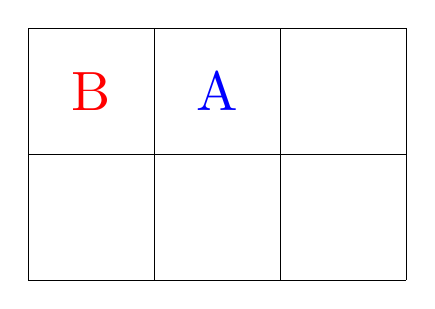
\begin{tikzpicture}[scale = 0.8]
            \draw (-3,2) -- (3,2);
            \draw (-3,-2) -- (3,-2);
            \draw (-3,0) -- (3,0);
            \draw (-3,-2) -- (-3,2);
            \draw (-1,-2) -- (-1,2);
            \draw (1,-2) -- (1,2);
            \draw (3,-2) -- (3,2);
            \node[red, scale = 2] (B) at (-2,1) {B};
            \node[blue, scale = 2] (A) at (0,1) {A};
        \end{tikzpicture}
        \qquad
        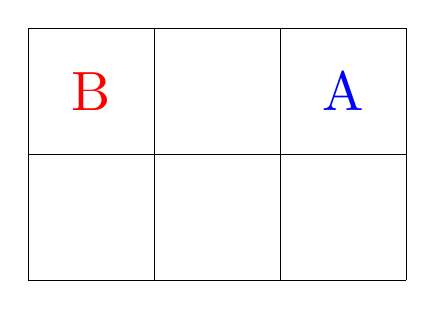
\begin{tikzpicture}[scale = 0.8]
            \draw (-3,2) -- (3,2);
            \draw (-3,-2) -- (3,-2);
            \draw (-3,0) -- (3,0);
            \draw (-3,-2) -- (-3,2);
            \draw (-1,-2) -- (-1,2);
            \draw (1,-2) -- (1,2);
            \draw (3,-2) -- (3,2);
            \node[red, scale = 2] (B) at (-2,1) {B};
            \node[blue, scale = 2] (A) at (2,1) {A};
        \end{tikzpicture}
    \end{center}

    \item 

    Describe what additional information the groupoid holds over the equivalence classes of configurations up to moves.
    
\end{enumerate}

\subsection{ Exercise 1.2 ( linear Yoneda Lemma 1) }

For an (associative and unital) ring $ R $ let $ B R $ be the category associated to the multiplicative monoid of $ R $.
Show that there is an isomorphism of categories $ \psi \colon \Mod_R \to \Fun_{ \mathbb{ Z } } ( ( B R )^{ \op } , \Ab ) $ relating the category of right $ R $-modules into the category of '$ \mathbb{ Z } $-linear presheaves over $ B M $', i.e. contravariant $ \mathbb{ Z } $-linear functors from $ B R $ to the category of abelian groups $ \Ab $.

\subsection{ Exercise 1.3 ( linear Yoneda Lemma 2 )}

Let $ R $ be a ring and let $ \prescript{  }{ R }{ R }_R$ be $ R $ viewed as an $ R $-$ R $-bimodule.

\begin{enumerate}[label=(\alph*)]

    \item 
    Show that for any $ R $-$ R $-bimodule $ N $ and any $ M \in \mod_R $ that $ \Hom_{ \mod R } ( N , M ) $ carries the structure of a right $ R $-module via $ ( f r ) ( x ) \coloneqq f ( r x ) $. 
    Deduce that $ N $ induces a functor
    \[
        \Hom_{\mod R } ( N , - ) \colon \mod R \to \mod R.
    \]
    
    \item 
    
    Show that there is an isomorphism of functors $ \Hom_{ \mod R } ( \prescript{}{ R }{ R }_R , - ) \cong \id_{ \mod R } $ given by evaluation at $ 1 \in R $.
\end{enumerate}

\subsection{ Exercise 1.4 (pullbacks in $\set$) }

Consider four sets $ A , B , C $ and $ E $ and assume that $ A , B \subseteq C $ with the inclusions $ \iota_A $ and $ \iota_B $.

\begin{enumerate}[label=(\alph*)]
    \item 
    Show that for any two maps $ \phi_A \colon E \to A $ and $ \phi_B \colon E  \to B $ such that $ \iota_A \circ \phi_A = \iota_B \circ \phi_B $ there is a unique map $ \phi \colon E \to A \cap B $ such that $ \phi_A = i_A \circ \phi $ and $ \phi_B = i_B \circ \phi $ for $ i_A $ and $ i_B $ the respective inclusions of $ A \cap B $. 
    \[
    \begin{tikzcd}
        E 
        \ar[rd, dashed, " \exists ! \phi" ]
        \ar[rrd, bend left, " \phi_A" ]
        \ar[rdd, bend right, " \phi_B" ']
        \\
        &
        A \cap B
        \ar[r , " i_A " ]
        \ar[d , " i_B " ]
        &
        A
        \ar[ d , " \iota_A" ]
        \\
        &
        B
        \ar[r, " \iota_B " ]
        &
        C
    \end{tikzcd}
    \]

    \item 
    Give an example of two maps $ f_A \colon A \to D $ and $ f_B \colon B \to D $ such that $ A \cap B $ does not have the above property for $ f_A $ and $ f_B $ instead of $ \iota_A $ and $ \iota_B $.

    \item 
    Show that in this more genral setting that
    \[
        A \times_D B \coloneqq \{ ( a, b ) \in A \times B \mid f_A ( a ) = f_B ( b ) \}
    \]
    with the canonical projections $ p_A, p_B$ satisfying the universal property from before.
    \[
    \begin{tikzcd}
        E 
        \ar[rd, dashed, " \exists ! \phi" ]
        \ar[rrd, bend left, " \phi_A" ]
        \ar[rdd, bend right, " \phi_B" ']
        \\
        &
        A \times_D B
        \ar[r , " p_A " ]
        \ar[d , " p_B " ]
        &
        A
        \ar[ d , " f_A" ]
        \\
        &
        B
        \ar[r, " f_B " ]
        &
        D
    \end{tikzcd}
    \]

    \item 
    What is the relation between $ A \cap B $ and $ A \times_C B$ for part (a) ?
\end{enumerate}


\section{Sheet 2}

\subsection{Exercise 2.1}

Show that two objects $ a , b \in A $ in a category $ A $ are isomorphic if and only if their respresentable presheaves $ \Hom_A ( - , a ) $ and $ \Hom_A ( -, b ) $ are isomorphic in $ \widehat{ A } $.

\subsection{Exercise 2.2}

Consider a functor $ F \colon A  \to \mathcal{ C } $ from a small category $A$.

\begin{enumerate}
    \item 
    Show that if $ A $ is an initial object $ \emptyset $, then the limit of $ F $ exists.

    \item 
    Show that if $ A $ has a final object $ e $, then the colimit of $ F $ exists.
\end{enumerate}

\subsection{Exercise 2.3}{ (limits and equalizers)}

Let $ F \colon A \to \set $ be a functor from a small category to the category of sets.
Recall that we have shown in the lecture that the limit of $ F $ exists and is given by 
\[
    \lim_A F \coloneqq \bigg\{ x \in \prod_{ a \in A } F ( a ) \mid \forall u \colon a \to b \quad F ( u ) ( x_a ) = x_b \bigg\}
\]
together with the canonical projections.

\begin{enumerate}[label=(\alph*)]
    \item 
    Show that the inclusion $ \lim_A F \subseteq \prod_{ a \in A } F ( a ) $ exhibits $ \lim_A F $ as the equalizer (= limit of the following diagram)
    \[
    \begin{tikzcd}
        \prod_{ a \in A } F ( a ) 
        \ar[r , shift left, " \phi "]
        \ar[r , shift right, " \psi "']
        &
        \prod_{ \substack{ u \colon s \to t \\ \text{ in } A} } F ( t )
    \end{tikzcd}
    \]
    where $ \phi ( x )_u = F ( u ) ( x_{ s ( u ) } ) $ and $ \psi ( x )_u = x_{ t ( u ) }$.

    \item 
    Let $ \coprod $ denote the disjoint union of sets. 
    Assume that the coequalizer ( = colimit of the following diagram ) 
    \[
    \begin{tikzcd}
        \coprod_{ \substack{ u \colon s \to t \\ \text{ in } A} } F ( t )
        \ar[r , shift left, " \phi "]
        \ar[r , shift right, " \psi "']
        &
        \coprod_{ a \in A } F ( a ) 
    \end{tikzcd}    
    \]
    exists where for $ y \in F ( s ( v ) ) \subseteq \coprod_{ \substack{ u \colon s \to t \\ \text{ in } A} } F ( t ) $ we have $ \phi ( y ) = F ( v ) ( y ) \in F ( t ( v ) ) \subseteq \coprod_{ a \in A } F ( a ) $ and $ \psi ( y ) = y \in F ( s ( v ) ) \subseteq \coprod_{ a \in A } F ( a ) $. Show that it is a colimit of $ F $ with the canonical maps fro $ F ( a ) $.
\end{enumerate}

\subsection{ Exercise 2.4 (colimits in Set) }
\begin{enumerate}[label=(\alph*)]
    \item 
    Show that the disjoint union of sets defines a coproduct in the category of sets, i.e. show that for every family of sets $ ( U_i )_{ i \in I } $ their disjoint union $\coprod_{ i \in I } U_i $ together with the canonical inclusion $ U_j \subseteq \coprod_{ i \in I } U_i $ is the colimit of the functor $ U \colon I \to \Set $ assigning to each $ i \in I $ the set $ U_i $.
    Here $ I $ is some indexing set.

    \item 
    Show that any coequalizer (= colimit of the following diagram ) 
    \[
    \begin{tikzcd}
        U 
        \ar[r, shift left, " \phi "]
        \ar[r, shift right, " \psi "']
        & 
        V
    \end{tikzcd}
    \]
    exists in Set by considering the smallest equivalence relation on $ V $ such that $ v \sim v' $ whenever there is some $ u \in U $ such that $ \phi ( u ) $ and $ \psi ( u ) = v' $.

    \item 
    Conclude using Exercise 2.3 that Set is cocomplete, i.e. every small colimit exists.
\end{enumerate}

\section{ Exercise 3.1 }

Consider two small categories $ A $ and $ B $ and a functor $ F \colon B \to \Fun ( A , \mathcal{ C } ) $. Assume further that $ \lim_B ( \ev_a \circ F ) $ exists in $ \mathcal{ C } $ for every $ a \in A $.

\begin{enumerate}[label=(\alph*)]
    \item 
    Show that a cone $ C $ of $ F $ is a limit cone if and only if for every $ a \in A $
    the evaluation $  C ( a ) $ is a limit cone of $ \ev_a \circ F $.

    \item 
    Deduce that for any small category $ A $ the category of presheaves $ \widehat{ A } $ is complete and cocomplete.

    \item 
    [Bonus] 
    We aim to show that the converse of the above is not true in general, i.e if not all
    $ \lim_B ( \ev_a \circ F ) $ exists, then $ \lim_B F $ might still exist ( and consequentially $( \lim_B F ) ( a ) $ is not a limit cone of $ \ev_a \circ F $ for some $ a \in A $.

    For this we will reformulate the property of a morphism being a monomorphism in terms of a pullback and show that there might exist monomorphisms in $ \Fun ( A , \mathcal{ C } )$ which are not pointwise monomorphisms. Fix $ A  \coloneqq \{ 0 < 1 \} $ to be the category with two objects and one morphism between them.
    Then $ \Fun ( A , \mathcal{ C } ) $ is the morphism category in $ \mathcal{ C } $.
    We now take $ \mathcal{ C } $ to be the category which does contain a non-monomorphism, explicitely let $ \mathcal{ C }$ be given by
    \[
    \begin{tikzcd}
        x 
        \ar[r, bend left, "f"]
        \ar[r, bend right, "g"']
        &
        y
        \ar[r, "h"]
        &
        z
    \end{tikzcd}
    \]
    with the relation $ h \circ f = h \circ g$.
    \begin{itemize}
        \item 
        Show that a morphism $ u \colon s \to t $ in a category is a monomorphism if and only if 
        \[
        \begin{tikzcd}
            s 
            \ar[d, "\id_s"]
            \ar[r, "\id_s"]
            &
            s
            \ar[d, "u"]
            \\
            s 
            \ar[r, "u"]
            & 
            u
        \end{tikzcd}
        \]
        is a pullback diagram.

        \item 
        Show that there is a monomorphism $ u \colon f \to h $ in $\Fun ( A , \mathcal{C} )$ such that $ u_1 $ is not a monomorphism.

        \item 
        Describe a $ B $ and a functor $ F  \colon B \to \Fun ( A , \mathcal{C} ) $ giving the desired counterexample.
        
    \end{itemize}
\end{enumerate}

\subsection{ Exercise 3.2 }

Let $ F \colon A \to \mathcal{ C } $ be a functor from a small category. Let $ \Tilde{ F } \colon A \to  \mathcal{ C } \to \widehat{ \mathcal{ C } } $ be the composition of $ F $ with the Yoneda embedding $ \mathcal{ C } \to \widehat{ \mathcal{ C } } $. Recall from Exercise 3.1 that the limit $ \lim_A \Tilde{ F } $ exists.

\begin{enumerate}[label=(\alph*)]
    \item 
    Show that there is a bijection between representations of $\lim_a \Tilde{ F } $ and limit cones of $ F $.

    \item 
    Deduce that the limit of $ F $ exists if and only if $ \lim_A \Tilde{ F } $ is representable, i.e. there exists some $ c_F \in \mathcal{ C } $ such that $ \lim_A  \Tilde{ F } \cong \Hom_{ \mathcal{ C } } ( - , c_F ) . $ 

    \item 
    Conclude that the Yoneda embedding $ \mathcal{ C } \to \widehat{ \mathcal{ C } } $ preserves limits.
\end{enumerate}

\subsection{Exercise 3.3}

Show that the inclusion $ \iota \colon \Gpd \to \Cat $ of small groupoids into the category of small categories has a right adjoint given by "forgetting" all non-isomorphisms in a given category.

\subsection{Exercise 3.4}

Let $ L \dashv R $ be an adjoint pair of functors where $ L \colon \mathcal{ C } \to \mathcal{ D } $.
Recall that we define unit $ \eta \colon \id_{ \mathcal{ C } } \to R \circ L $ the image of $ \id_{ L ( c ) } $ under the adjunction isomorphism
\[
    \phi_{ ( c , L ( c ) ) } \colon \Hom_{\mathcal{ D } } ( L ( c ) , L ( c ) ) \cong \Hom_{ \mathcal{ C } }( c, R ( L ( c ) ) )
\]
for every $ c \in \mathcal{ C } $ and the counit $ \epsilon \colon L \circ R \to \id_{ \mathcal D } $ as the image of $ \id_{ R ( d ) } $ under the adjunction isomorphism
\[
    \phi^{ -1 }_{ ( R ( d ) , d ) } \colon \Hom_{ \mathcal{ C } } ( R ( d ) , R ( d ) ) \cong  \Hom_{ \mathcal{ D } }( L ( R ( d ) ) , d ) 
\]
for every $ d \in \mathcal{ D } $. 
Show the following 
\begin{enumerate}
    \item 
    The assignment $ \epsilon $ is indeed a natural transformation.

    \item 
    Without using $ L \dashv R $, show that $ \Tilde{ \phi }_{ ( c ,d ) } \coloneqq \eta_c^* \circ R_{ L ( c ) , d } $ defines a natural transformation
    \[
        \Tilde{ \phi } \colon \Hom_{ \mathcal{ D } }( L ( - ) , ?  ) \to \Hom_{ \mathcal{ C } } ( - , R ( ? ) ). 
    \]

    \item 
    There is an adjunction $ R^{ \op } \dashv L^{ \op } $ between the opposite categories with uni $ \epsilon^{ \op } \colon \id_{ \mathcal{ D }^{ \op } } \to L^{ \op } \circ R^{ \op } $ and counit $ \eta^{ \op } \colon R^{ \op } \circ L^{ \op } \to \id_{ \mathcal{ C  }^{\op} } $.

    \item 
    For any $ d \in \mathcal{ D } $ the category $ L / d $ has the final object $ ( R ( d ) , \epsilon_d \colon L R ( d ) \to d ) $.

    \item 
    Given a second adjunction $ L' \dashv R' $ with $ L' \colon \mathcal{ D} \to \mathcal{ A } $ and a unit $ \eta' $ and counit $ \epsilon' $, the counit of the composed adjunction $ L' \circ L \dashv R  \circ R' $ is given by $ \epsilon'_{ ( - ) } \circ L' ( \epsilon_{ R' ( - ) } ) $.

    \item 
    Any right adjoint $ R' $ of $ L , L \dashv R' $, is isomorphic to $ R $.
\end{enumerate}

\section{Exercise sheet 4}

\subsection{Exercise 4.1}
Let $ L \colon \mathcal{ C } \to \mathcal{ D } $ be a functor between small categories.

\begin{enumerate}[label=(\alph*)]
    \item 
    For $ d \in \mathcal{ D } $ describe the category of elements of the presheaf $\Hom_{\mathcal{ D } } ( L ( - ) , d ) \in \widehat{ \mathcal{ C } }$.

    \item 
    Show that $ L $ admits a right adjoint if and only if for every $d \in \mathcal{ D } $ the category of elements $ \int^{ \mathcal{ C } } \Hom_{ \mathcal{ D } } ( L ( - ) , d ) $ admits a final object.
\end{enumerate}

\subsection{Exercise 4.2}
Let $ A $ be a small category and $ a \in A $ some object.

\begin{enumerate}[label=(\alph*)]
    \item 
    Show that $ \Hom_{\widehat{A}}( \widehat{a} , - ) \colon \widehat{A} \to \Set $ preserves colimits, i.e. for any functor $ F \colon I \to \widehat{ A } $ the canonical map 
    \[
        \colim_I ( \Hom_{ \widehat{ A } } ( \widehat{ a } , - ) \circ F ) \to \Hom_{ \widehat{ A } }( \widehat{ a }, \colim_I F )
    \]
    is an isomorphism.

    \item 
    Deduce that $\Hom_{\widehat{A}} ( \widehat{a} , - ) $ admits a right adjoint and describe it.
\end{enumerate}

\subsection{4.3}
Let $ u \colon A \to  B $ be a functor between small categories. 
Let $ u* \colon \widehat{ B } \to \widehat{ A } $ denote the functor obtained by precomposition with $ u $.

\begin{enumerate}[label=(\alph*)]
    \item 
    Show that $u^*$ preserves colimits.

    \item 
    Deduce that there exists a right adjoint $ u^* \dashv u_* $.

    \item 
    Give an explicit description of $ u _*$.

    \item 
    Confirm directly that $ u^* \dashv u_* $ by giving the adjunction isomorphism explicitly.
\end{enumerate}

\subsection{Exercise 4.4}

Let $ X $ be a presheaf over a small category $ A $. Recall from the lecture the canonical functor.
\[
    u \colon \int^A X \to \widehat{ A } / X 
\]
sending $ ( a , s \in X_a ) $ to $ s \colon \widehat{ a } \to X $, where $ \int^A X $ is the category of elements of $ X $. 
Hence, by extending by colimits we obtain a functor
\[
    u_! \colon \widehat{\int^A X} \to \widehat{A} / X
\]
which we aim to show is equivalence, most of which was done in the lecture. 
Show the remaining claims.

\begin{enumerate}[label=(\alph*)]
    \item 
    The slice category $ \widehat{A} / X $ is cocomplete.

    \item 
    For any $ ( a , s \colon a \to X ) \in \int^A X $ the functor $ \Hom_{\widehat{A}/X} ( u_! ( \widehat{ ( a ,s )} ) , - ) $ preserves colimits.

    \item 
    Any $ ( Y , f \colon Y \to X ) $ can be obtained as a colimit of a diagram in the essential image of $ u $.
\end{enumerate}

\section{ Exercise Sheet 5 }

\subsection{ Exercise 5.1}

Let $ \mathcal{ C } $ and $ \mathcal{ D } $ be two cocomplete categories where $ \mathcal{ C } $ is small and let $  D \colon I \to \mathcal{ C } $ be a diagram in $ \mathcal{ C } $.

\begin{enumerate}[label=(\alph*)]
    \item 
    Show that there is a natural transformation of functors $ \Fun ( \mathcal{ C }, \mathcal{ D } \to \mathcal{ D } $
    \[
        can \colon \colim_I D^* ( - ) \to \ev_{ \colim_I D}.
    \]
    
    \item 
    Deduce that if $ F $ and $ G $ are two isomorphic funtors in $ \Fun ( \mathcal{ C } , \mathcal{ D } ) $, then $ F $ is colimit preserving if and only if $ G $ is.
\end{enumerate}

\subsection{ Exercise 5.2}

Consider an adjunction $ L \dashv R $ where $ L \colon \mathcal{ C } \to \mathcal{ D } $.

\begin{enumerate}[label=(\alph*)]

    \item 
    Show that for a $ d \in \mathcal{ D } $ the counit $ \epsilon_d $ at $ d $ is an isomorphism if and only if $ R $ induces a natural isomorphism 
    \[
        R_{d,-}\colon \Hom_{\mathcal{ D } } ( d, - ) \to \Hom_{ \mathcal{ C } } ( R ( d ) , R ( - ) ). 
    \]

    \item 
    Deduce that $ R $ is fully faithful if and only if the counit $ \epsilon \colon L \circ R  \to \id_{\mathcal{ D } } $ is an isomorphism.

    \item 
    Give the dual statement to (b) and give a proof reducing the statement to (b).

    \item 
    Show that if $ R $ is fully faithful, then $ c \in \mathcal{ C } $ is in the essential image of $ R $ if and only if the unit morphism $ \eta_c $ is an isomorphism at $ c $.
    
\end{enumerate}

\subsection{ Exercise 5.3 }

Let $ u \colon A \to B $ be a functor between small categories.
Recall from the lecture and Exercise 4.3 that we have a triple of adjunctions $ u_! \dashv u^* \dashv u_* $ where $ u^* \colon  \widehat{ B } \to \widehat{ A } $. 
Assume further that $ u $ is fully faithful.

\begin{enumerate}[label=(\alph*)]

    \item 
    Show that $ u_* $ is fully faithful. 

    \item   
    Show that $ u_! $ is fully faithful.
    \newline
    (Hint: Show that the class $ \{ X \in \widehat{ A } \mid \eta_X \text{ is invertible } \} $ is closed under colimits and contains all representable presheaves.)
    
\end{enumerate}

\subsection{ Exercise 5.4 }

Show that the functor $ \widehat{ \Delta }  \to \SetD $ which remembers only the face and degeneracy maps and is the identity on morphisms is an isomorphism of categories. 
In particular,
 \begin{itemize}
     \item 
     show that the functor is well defined by showing that the co-face and co-degeneracy maps satisfy the cosimplicial identities.
     \begin{align*}
         d^jd^i &= d^i d^{j-1} \quad \text{ if } i < j
         \\
         s^j s^i &= s^i s^{j+1} \quad \text{ if } i \leq j
     \end{align*}
     \qquad
     $
     s^j d^i=
     \begin{cases}
         d^i s^{j-1} &\text{ if } i < j 
         \\
         \id &\text{ if } i \in \{ j , j + 1 \}
         \\
         d^{i-1} s^j &\text{ if } i > j = 1
     \end{cases}
     $
     Recall that the co-face maps $ d^i \coloneqq d_n^i $ and co-degeneracy maps $ s^i \coloneqq s_n^i $ are defined as follows for each $ n \in \mathbb{ N }_+ $ respective $ n \in \mathbb{ N }_0 $ and $ 0 \leq i \leq n $.  
     \begin{align*}
         d^i = d_n^i \colon [ n - 1 ] &\to [ n ]
         \\
         k &\mapsto 
         \begin{cases}
             k & \text{ if } k < i 
             \\
             k+1 & \text{ if } i \leq k 
         \end{cases}
     \end{align*}
     \quad
     \begin{align*}
         s^i = s_n^i \colon [ n n 1 ] &\to [ n ]
         \\
         k &\mapsto 
         \begin{cases}
             k & \text{ if } k \leq i 
             \\
             k-1 & \text{ if } i < k 
         \end{cases}
     \end{align*}

     \item  
     For the inverse, show that a morphism $ \sigma \colon [m] \to [n] $ in $ \Delta $ can be uniquely written as
    \[
        \sigma 
        =
        d_n^i_s
        \circ d_{ n - 1 }^{i_{s-1}} 
        \circ 
        \dotsm 
        \circ
        d_{ n - s + 1 }^{i_1}
        \circ
        s_{ m - t }^{j_1}
        \circ 
        \dotsm
        \circ
        s_{ m - 2 }^{ j_{t-1}}
        \circ 
        s_{ m - 1 }^j_t
    \]
    with $ 0 \leq i_1 < i_2 < \dotsm < i_s \leq n $ and $ 0 \leq j_1 < j_2 < \dotsm < j_t < m $ and $ n-s = m-t $.
\end{itemize}

\section{ Exercise sheet 6 }

\subsection{ Exercise 6.1 }

Fix $ n \in \mathbb{ N }_+ $.
Define the simplicial subset $ \partial \Delta^n \subseteq \Delta^n $ by
\[
    \partial \Delta^n ( [ m ] ) \coloneqq \{ \sigma \colon [ m ] \to [ n ] \text{ non-surjective } \}
\]
and similarly, define for $ 0 \leq k \leq n $ the simplicial subset $ \Lambda_k^n \subseteq \partial \Delta^n $ by
\[
    \Lambda_k^n( [ m ] ) \coloneqq \{ \sigma  \in \partial \Delta^n ( [ m ] ) \mid \sigma ( [ m ] ) \neq [ n ] \setminus \{ k \} \}.
\]
\begin{enumerate}[label=(\alph*)]
    
    \item 
    Confirm that the above are indeed simplicial subsets.

    \item 
    Show one of the following 
    \begin{itemize}
    
        \item 
        $ \partial \Delta $ is the smallest simplicial subset of $ \Delta^n $ such that $ \{ d_n^i \mid 0 \leq i \leq n \} \subseteq \partial \Delta^n ( [ n - 1 ] ) $.

        \item 
        $\Lambda_k^n$ is the smallest simplicial subset of $ \Delta^n $ such that $ \{ d_n^i \mid 0 \leq i \leq n \wedge i \neq k \} \subseteq \Lambda^n_k ( [ n - 1 ] )$.
        
    \end{itemize}

Recall that we may view $ \Delta $ as a category of posets, so that we may compute the nerve of ( subsets of ) $ [ n ] $ as partially ordered set.
Moreover, we may associate to $ [ n ] $ the category $ \Sub_* ( [ n ] ) $ of non-empty proper full subcategories, i. e. $ [ n ] \notin \Sub_* ( [ n ] ) $, and morphisms given by inclusions.
Similarly, we define for $ k \in [ n ] $ the full subcategory $ \Sub_*^k ( [ n ] ) \coloneqq \{ k \in E \in \Sub_* ( [ n ] ) \subseteq  \Sub_* ( [ n ] )$.

    \item 
    Show one of the following.

    \begin{enumerate}
        \item 
        \[
            \partial \Delta^n
            \cong 
            \bigcup_{ E \in \Sub_* ( [ n ] ) } N ( E ) \coloneqq 
            \colim_{ E \in \Sub_* ( [ n ] ) } N ( E ) 
        \]

        \item 
        \[
            \partial \Delta^n
            \cong
            \bigcup_{ E \in \Sub_* ( [ n ] ) } N ( E ) \coloneqq 
            \colim_{ E \in \Sub_* ( [ n ] ) } N ( E ) 
        \]
    \end{enumerate}

    \item 
    Justify the notation $ \bigcup $.
    
\end{enumerate}

\subsection{ Exercise 6.2 }

Let $ \Delta_{ \leq n } $ be the full subcategory of $ \Delta $ of the elements $ [ 0 ] , [ 1 ] , \dotsc , [ n ] $.
The inclusion $ \iota_n \colon \Delta_ { \leq n } \to \Delta $ induces a truncation functor $ \tr_n \coloneqq ( \iota_n )^* \colon \Set_{ \Delta } \to \widehat{ \Delta_ { \leq n } } $.

\begin{enumerate}[label=(\alph*)]
    
    \item 
    Show that $ \tr_n $ admits both a left and a right adjoint, $ \sk_n \dashv \tr_n \dashv \cosk_n $, which are both fully faithful.

    \item 
    Deduce that we have an adjunction $ \bold{sk_n} \coloneqq \sk_n \circ \tru_n \dashv \cosk_n \circ\tru_n \eqqcolon \bold{ cosk_n } $ of endofunctors of $ \SetD $.
    
\end{enumerate}

The essential image of $ \sk_n $ are called the $ n $-skeletal simplicies while the essential image of $ \bold { cosk_n } $ are the $ n $-coskeletal simplices.

\begin{enumerate}[label=(\alph*), resume]
    \item 
    Show that a simplicial set $ X $ is $ n $-skeletal if and only if 
    
    $ \tru_n \colon \Hom_{ \SetD } ( X , - ) \to \Hom_{ \widehat{ \Delta{ \leq n }}} ( \tru_n X , \tru_n ( - ) ) $ is an isomorphism of functors.

    \item 
    Show that a simplicial set $ Y $ is $ n $-coskeletal if and only if
    
    $ \tru_n \colon \Hom_{ \Set_\Delta } ( - , Y ) \to \Hom_{ \widehat{ \Delta_{ \leq n }} } ( \tru_n ( - ) , \tru_n Y ) $ is an isomorphism of functors.
\end{enumerate}

\subsection{ Exercise 6.3 }

\begin{enumerate}[label=(\alph*)]
     
     \item 
     Show that a map $ F \colon X  \to N ( \mathcal{ C } ) $ to the nerve of a category $ \mathcal{ C } $, is completely determined by a map $ u \colon X_1 \to \Mor ( \mathcal{ C } ) $ such that 
     \begin{enumerate}
         \item 
         for all $ x \in X_0 $ we have that $ u ( s_0 ( x ) ) $ is an identity and 

         \item 
         for any $2$-simplex $ \sigma \in X_2 $ we have that $ u ( d_1 ( \sigma ) ) = u ( d_0 ( \sigma ) ) \circ u ( d_2 ( \sigma ) )$.
     \end{enumerate}

     \item 
     Deduce that the nerve of a category is 2-coskeletal.

     \item 
     Conclude that the nerve $ N \colon \Cat \to \SetD $ is fully faithful.
     
\end{enumerate}

\subsection{ Exercise 6.4 }

Consider the functor $ \Op \colon \Delta \to \Delta $ which is the identity on objects and for $ \sigma : [ n ] \to [ m ] $
\[
    \Op ( \sigma ) ( i ) 
    \coloneqq
    m - \sigma ( n - i )
\]
Let $ ( - )^{ \op } \coloneqq \Op^* \colon \SetD \to \SetD $ be the corresponding involution of the category of simplicial sets.

\begin{enumerate}[label=(\alph*)]
    \item 
    Show that $ \Op $ is a well defined involution.

    \item 
    For a simplicial set $ X $, describe the face and degeneracy maps of $ X ^{ \op } $.

    \item 
    Show that for a category $ \mathcal{ C } $ we have an isomorphism $ N ( \mathcal{ C }^{\op} ) \cong N ( \mathcal{ C } )^{\op} $.

    \item   
    Show that for a topological space there is an isomorphism $ \Sing ( X ) \cong \Sing ( X )^{ \op } $ for the singular complex of $ X $.
\end{enumerate}

\section{Exercise Sheet 7}

\subsection{Exercise 7.1}

Recall that we defined the connected component functor $ \pi_0 : \SetD \to \Set $ as 
\[
    \pi_0 ( X ) \coloneqq \colim_{ \Delta } X 
\]
which yields a left adjoint to the constant diagram functor $ \const : \Set \to \SetD $.

\begin{enumerate}[label=(\alph*)]
    
    \item 
    Show that $ \pi_0 ( \Delta^n ) $ is a one point set for any $ n \in \mathbb{ N } $.

    \item 
    Recall from Exercise 6.1 the boundaries $ \partial \Delta^n $ and horns $ \Lambda_k^n $ of $ \Delta^n $.
    Compute $ \pi_0 ( \partial \Delta^n ) $ and $ \pi_0 ( \Lambda_k^n ) $. 
\end{enumerate}

By definition the connected components of a small category $ \mathcal{ C }$ are defined as the coequalizer 
\[
    \begin{tikzcd}
    \Mor ( \mathcal{ C } ) 
    \ar[r, shift left, "\text{target}"]
    \ar[r, shift right, "\text{source}"']
    &
    \Ob( \mathcal{ C } )
    \end{tikzcd}
\]

\begin{enumerate}[label=(\alph*), resume]
   
    \item 
    Show that for any simplicial set $ X $, the connected components $ \pi_0 ( X ) $ of $ X $ agree with the connected components of the category of elements $ \int^{ \Delta } X $.

    \item 
    Show that the connected components of a category $ \mathcal{ C } $ agree with the connected components of its nerve $ \pi_0 ( N ( \mathcal{ C } ) )$.
    
\end{enumerate}

\subsection{Exercise 7.2}

For a simplicial set $ X $, let $\bold{ Sk_n } ( X ) $ be the smallest simplicial subset of $ X $ such that $ ( \bold{ Sk_n } ( X ) )_m = X_m $ for $ m \leq n $.

\begin{enumerate}
    \item 
    Show that there is a natural isomorphism $ \bold { Sk_n } ( X ) \cong \bold { sk_n } ( X ) $, i.e. $ \bold{ Sk_n } $ describes the $n$-skeleton functor from Exercise 6.2.
\end{enumerate}

Consider for any simplicial set $ X $ the canonical functor $ \bold{ sk }_X \colon \mathbb{ N }_0 \to \SetD $ with $ \bold{ sk }_X ( n ) \coloneqq \bold{ sk }_n ( X ) $ and morphisms induced by the inclusion $ \bold{ sk }_n ( X ) \subseteq X $.
We call the image of $ \bold{ sk }_X $ the skeletal filtration of $ X $. 
For convenience, we set $ \bold{ sk }_{-1} ( X ) $ to the empty presheaf.

\begin{enumerate}[label=(\alph*), resume]
    \item 
    Argue that the morphisms in the skeletal filtration of $ X $ are monomorphisms and show that $ X \cong \colim_{ \mathbb{ N } } \bold{ sk }_X$.

    \item 
    Recall that $ \sigma \in X_n $ can be viewed as a morphism $ \sigma : \Delta^n \to X $.
    Observe that $ \sigma $ factors through $ \bold{ sk }_n ( X ) $ and that the precomposition of $ \sigma $ with the inclusion $ \partial \Delta^n \subseteq \Delta $ factors through $ \bold{ sk }_{n-1} ( X ) $.
    Show that these maps assemble into a pushout diagram.
    \begin{tikzcd}
        \coprod_{ \sigma \in X_n^{nd}} \partial \Delta^n
        \rar
        \dar
        &
        \coprod_{ \sigma \in X_n^{nd}} \Delta^n
        \dar
        \\
        \bold{sk_{n-1}}(X)
        \rar
        &
        \bold{sk_n}(X)
    \end{tikzcd}
    Here $X_n^{\nd} \coloneqq X_n \setminus ( \bold{ sk_{n-1} ( X ) })_n$ 
    denotes the set of non-degenerate $n$-simplicies in $ X$

    \item   
    Show that the geometric realisation of a simplicial set is a CW complex.
\end{enumerate}

\subsection{Exercise 7.3}

\begin{enumerate}[label=(\alph*)]
    
    \item 
    Show that for $ n \in \mathbb{N}_0 $ we have $ \bold{sk}_n ( \Delta^{n+1} ) \cong \partial \Delta^{n+1}$.

    \item 
    Show that for every horn $ \Lambda_k^m $ we have that 
    \[
        \bold{sk_n} ( \Lambda_k^m ) \cong 
        \begin{cases}
            \Lambda_k^m &\text{ if } m \leq n+1
            \\
            \bold{sk}_n ( \Delta^m ) &\text{ if } m > n+1
        \end{cases}
    \]
    for $ 0 \leq k \leq m \in \mathbb{ N }_+$.

    \item 
    Show that for a Kan comlex $ K $ and any $ n \in \mathbb{N}_0 $, the $ n $-coskeleton $\bold{cosk}_n ( K ) $ is a Kan complex.
    
\end{enumerate}

\subsection{Exercise 7.4}
\begin{enumerate}[label=(\alph*)]
    \item 
    Show that the class of Kan complexes and the class of inner Kan complexes are closed under set indeced products.

    \item 
    Show that a set indexed product of connected Kan complexes is connected.

    \item 
    Give an example that an infinite product of connected inner Kan complexes is not necessarily connected. 
    ( Recall that the nerve of a category is an inner Kan complex.)
\end{enumerate}

\section{Exercise sheet 8}

\subsection{Exercise 8.1}

Fix an inner Kan complex $ X $. For edges $ f , g , h \in X_1 $ we say $ g \cdot f \sim h $ if there exists a 2 simplex such that $d_0 ( \sigma ) = g , d_1 ( \sigma ) = h $ and $ d_2 ( \sigma ) = f $.

\begin{enumerate}
    \item 
    Show Joyal's Coherence Lemma:

    Consider $ \alpha: \bold{sk}_1 ( \Delta^3 ) \to X $ with $ \alpha_1 ( f_{21} ) \cdot \alpha_1 ( f_{10} ) \sim \alpha_1 ( f_{20} ) $ and $ \alpha_1 ( f_{32} ) \cdot \alpha_1 ( f_{21} ) \sim \alpha_1 ( f_{31} )$.
    Then $ \alpha_1 ( f_{31} ) \cdot \alpha_1 ( f_{10} ) \sim \alpha_1 ( f_{30} )$ if and only if $ \alpha_1 ( f_{32} ) \cdot \alpha_1 ( f_{20} ) \sim \alpha_1 ( f_{30} ) $.
    Here we denote by $ f_{ji} $ the unique morphism $ f_{ i , j } : [1 ] \to [ 3 ]$ with image $ \{ i < j \} \subseteq [ 3 ] $.
\end{enumerate}

We define the following four relations on $X_1$.

\begin{align*}
    f \sim_1 g & \iff f \cdot s_0 ( d_1 ( f ) ) \sim g 
    \\
    f \sim_3 g & \iff g \cdot s_0 ( d_1 ( g ) ) \sim f
\end{align*}
\qquad
\begin{align*}
    f \sim_2 g & \iff f \cdot s_0 ( d_0 ( f ) ) \sim g 
    \\
    f \sim_4 g & \iff g \cdot s_0 ( d_0 ( g ) ) \sim f
\end{align*}

\begin{enumerate}[label=(\alph*), resume]
    \item 
    Show that $ f \sim_1 g \iff f \sim_2 g $ and that $ f \sim_1 g \implies f \sim_3 g $.

    \item 
    Deduce that all four relations agree.

    \item 
    Conclude that the relation $ \simeq \coloneqq \sim_1 $ is an equivalence relation on $X_1$.
\end{enumerate}

\subsection{Exercise 8.2}

Show that the homotopy category $ \Ho ( N ( \mathcal{ C } ) ) $ of the nerve of a small category $ \mathcal{ C } $ is isomorphic to $ \mathcal{ C } $.

\subsection{ Exercise 8.3 }

Let $ G $ be a simplicial group.
Let $ n \in \mathbb{ N }_+ $ and $ 0 < l < n+1 $. 
For $ y \in G_{n+1} $ we say $ x \in G_n $ is $l$-compatible if $ d_i ( x ) = d_l ( d_{i+1} ( y ) ) $ if $ l \leq i $. 
Moreover, we say $x$ is $ ( k , l ) $-compatible for $ 0 \leq k < l $ if additionally $ d_i ( x ) = d_{ l-1 } ( d_i ( y ) ) $ for $ 0 \leq i < k $.

\begin{enumerate}[label=(\alph*)]
    \item 
    Show that if $ x $ is $ ( k , l ) $-compatible with $ y \in G_{n+1} $, then we have for $ y' \coloneqq s_{l-1} ( x \cdot ( d_l ( y ))^{-1} ) \cdot y  \in G_{n+1} $ that 
    \[
    d_i ( y' ) =
    \begin{cases} 
        d_i(y) &\text{ if } k < l
        \\
        x &\text{ if } i = l 
        \\
        d_i ( y ) &\text{ if } i > l
    \end{cases}
    \]

    \item 
    Give the notion of cocompatibility which is dual to compatibility.

    \item 
    Show that the underlying simplicial set of $ G $ is a Kan complex.
    
\end{enumerate}

\subsection{Exercise 8.4}

Recall from Exercise 6.2 the definition of the $n$-coskeleton of a simplicial set $ X $ and $ n \in \mathbb{N}_0 $.

\begin{enumerate}[label=(\alph*)]
    \item 
    Show that if $ X $ is $n$-coskeletal, then for any $ m > n $ we have an isomorphism
    \[
        \Hom_{\SetD}( \Delta^m , X ) 
        \to 
        \Hom_{\SetD} ( \partial \Delta^m , X ) 
    \]
    induced by the inclusion $ \partial \Delta^m \subseteq \Delta^m$.

    \item 
    Show that if for some $ m \in \mathbb{N}_+$ the inclusion $ \partial \Delta^m \subseteq \Delta^m $ induces an isomorphism for $ X $ as above, then for any morphism $ Y \to X $ of simplicial sets, the component $ f_m \colon Y_m \to X_m $ is completely determined by $ \tru_{m-1} ( f ) $.

    \item 
    Conclude that a simplicial set $ X $ is $ n $-coskeletal if and only if for every $ m > n $ the inclusion $ \partial \Delta^m \subseteq \Delta^m $ induces an isomorphism $ \Hom_{ \SetD } ( \Delta^m , X ) \to \Hom_{\SetD} ( \partial \Delta^m , X )$.
    
\end{enumerate}

\section{Exercise sheet 9}

\subsection{Exercise 9.1}

Recall that for a category $ \mathcal{ C } $ and a class of morphisms $ \mathcal{ F } \subseteq \Mor ( \mathcal{ C } )$ the class of morphisms with the left lifting property with respect to $ \mathcal{ F } $ is 
\[
    l ( \mathcal{ F } )
    \coloneqq  
    \Bigg\{ i \colon x \to y \mid \forall \begin{tikzcd}
        a 
        \ar[r, "f"]
        \ar[d, "i"]
        &
        x
        \ar[d, "p \in \mathcal{ F }"]
        \\
        b
        \ar[r, "g"]
        &
        y
    \end{tikzcd}
    \exists h
    \begin{tikzcd}
        a 
        \ar[r, "f"]
        \ar[d, "i"]
        &
        x
        \ar[d, "p "]
        \\
        b
        \ar[r, "g"]
        \ar[ru, dashed, "h"]
        &
        y
    \end{tikzcd}
    \Bigg\}
\]
where diagrams commute, i.e. $ p \circ f = g \circ i , f = h \circ i $ and $ g = p \circ h $.
\begin{enumerate}[label=(\alph*)]
    \item 
    Give the explicit description of the class of morphisms with the right lifting property of $ \mathcal{ F } , l ( \mathcal{ F } )$, which is defined dually, i.e.
    \[
        r ( \mathcal{ F } ) \coloneqq ( l ( \mathcal{ F^{\op} } ) )^{\op}
    \]
    where $\mathcal{ F }^{\op} $ denotes the same class of morphisms but viewed in the opposite category $ \mathcal{ C }^{\op}$.

    \item 
    Show that $ l ( r ( l ( \mathcal{ F } ) ) ) = l ( \mathcal{ F } ) $.

\end{enumerate}

From now on let $ \mathcal{ C } = \Set $ and consider the inclusion $ \iota : \emptyset \to \{ \star \} $ of the empty set into a set with one element.

\begin{enumerate}[label=(\alph*), resume]
    \item 
    Compute the set of morphisms with the right lifting property for $ \iota, r ( \{ \iota \} ), $ in Set.

    \item 
    Show that $ l ( r ( \{ \iota \} ) ) $ is the class of injective maps.

    \item 
    Show that (d) is equivalent to the axiom of choice.
    \[
        \forall  X ( \emptyset \notin X \implies \exists \varphi \colon X  \to \bigcup_{ A \in X } A 
        \forall A \in C \varphi( A ) \in A )    
    \]
\end{enumerate}

\subsection{ Exercise 9.2 }

Let $ \mathcal{ F } $ be a class of morphisms in a cocomplette category $ \mathcal{ C } $.
We say that an object $ x \in \mathcal{ C } $ is a retract of an object $ y \in \mathcal{ C } $ if there exist two morphisms $ j : x \to y $ and $ q: y \to x $ such that $ q \circ j = \id_x .$

\begin{enumerate}[label=(\alph*)]
    \item 
    Describe retracts in the category of morphisms $ \Fun ( [ 1 ] , \mathcal{ C } ) $ where we assume $ \mathcal{ C } $ to be small.

    \item 
    Show that $ l ( \mathcal{ F } ) $ is closed under retracts in the sense (a).

    \item 
    Show that $ l ( \mathcal{ F } ) $ is closed under pushouts, i.e. for any pushout square
    \[
    \begin{tikzcd}
        x 
        \ar[r, "g"]
        \ar[d, "f"]
        &
        x'
        \ar[d,"f'"]
        \\
        y
        \ar[r, "g'"]
        &
        y'
    \end{tikzcd}
    \]
    we have that if $ f \in l ( \mathcal{ F } ) $, then $ f' \in l ( \mathcal{ F } ) $.

    \item 
    Show that $ l ( \mathcal{ F } )$ is closed under composition.

    \item 
    Show that $ l ( \mathcal{ F } ) $ is closed under ( countable ) transfinite composition, i.e. for any functor $ F : \mathbb{ N }_0 \to \mathcal{ C } $ with $ f_n \coloneqq F ( n < n + 1 ) \in l ( \mathcal{ F } ) $ we have that the canonical map $ F ( 0 ) \to \colim_{ \mathbb{ N } } F $ is in $ l ( \mathcal{ F } ) $.
\end{enumerate}

Note that (e) can be generalised to arbitrary well-ordered sets (ordinals) in place of $ \mathbb{ N } $ using transfinite induction.

\subsection{ Exercise 9.3 }

Let $ \mathcal{ F } $ be a class of morphisms on a cocomplete category $ \mathcal{ C } $.
Assume that $ \mathcal{ F } $ includes all identity morphisms, is closed under pushouts and (countable) transfinite composition in the sense of Exercise 9.2.

\begin{enumerate}[label=(\alph*)]
    \item 
    Show that $ \mathcal{ F } $ contains all isomorphisms.

    \item 
    Show that $ \mathcal{ F } $ is closed under composition.

    \item 
    Deduce that $ \mathcal{ F } $ is closed under finite coproducts, i.e. for two morphisms $ f : x  \to y $ and $ f' : x' \to y' $ with both $ f , f' \in \mathcal{ F } $, we have that the induced map $ f \amalg f' : x \amalg x' \to y \amalg y' $ is also in $ l ( \mathcal{ F } ) $.

    \item 
    Show that $ \mathcal{ F } $ is closed under countable coproducts by expressing a morphism $ \coprod_{ n \in \mathbb{ N } } f_n $ as suitable transfinite composition.
    
\end{enumerate}

Again, assuming that $ \mathcal{ F } $ is closed under arbitrary transfinite compositions, we can generalise the above argument to show that $ \mathcal{ F } $ is closed under set indexed coproducts.

\subsection{ Exercise 9.4 }

Let $ A $ be a small category. 
Recall that a morphism $ f : y \to z $ in $ A $ is a monomorphism, if for any two $ g , g' : x \to y $, we have that $ f \circ g = f \circ g' $ if and only if $ g = g' $.

\begin{enumerate}[label=(\alph*)]
    \item 
    Show that a morphism in $ \Set $ is a monomorphism if and only if it is injective.

    \item 
    Deduce from Exercise 3.1 that a morphism of presheaves $ f : X \to Y $ in $ \widehat{ A } $ is a monomorphism if and only if $ f_a $ is a monomorphism for all $ a \in A $.

    \item 
    Conclude that the class of monomorphism in $ \widehat{ A } $ is closed under retracts, pushouts, (countable) transfinite composition and coproducts. In particular, the class of monomoprhism in $ \widehat{ A } $ is saturated.
\end{enumerate}

\section{ Exercise sheet 10 }

\subsection{Exercise 10.1}

We define the class of trivial Kan fibrations to be $ r ( \{ \partial \Delta^n \to \Delta^n \mid n \in \mathbb{ N }_0 \} ) $ in $ \SetD $.
Furthermore, let $ \mathcal{ F } $ be the smallest saturated class containing all boundary inclusions $ \{ \partial \Delta^n \to \Delta^n \mid n \in \mathbb{ N }_0 \} $.

\begin{enumerate}[label=(\alph*)]
    \item 
    Show that $ r ( \mathcal{ F } ) $ is the class of trivial Kan fibrations.

    \item 
    Show that $ \mathcal{ F } $ contains all monomorphisms. Proceed as follows.

    \begin{itemize}
        \item 
        For a fixed monomorphism $ \iota : X \to Y $ construct a filtration of $ Y $ by $ X \cup \bold{sk_{n-1}} ( Y ) $ starting with $ X = X \cup \bold{sk_{-1}}( Y ) $, similar to the skeletal filtration from Exercise 7.2. 
        Here $ X \cup \bold{sk_n} ( Y ) $ is defined as pushouts of $ \bold{ sk_n } ( Y ) $ and the image of $ \iota $ along their intersection.

        \item 
        Observe that $ \iota $ is the transfinite composition of this filtration.

        \item 
        Show that the morphisms $ X \cup \bold{sk_{n-1]}}( Y ) \to X \cup \bold{ sk_n }( Y ) $ is pushout of morphisms in $ \mathcal{ F } $ for all $ n \in \mathbb{ N }_0 $ by construction a similar pushout diagram as for the skeletal filtration.
    \end{itemize}

    \item 
    Deduce that $\mathcal{ F }$ is the class of monomorphisms.

    \item 
    Conclude that a trivial Kan fibration is a Kan fibration.
    
\end{enumerate}

\subsection{Exercise 10.2}

We have shown in the lecture that the saturated closure of the horn inclusions 
\[
    \mathcal{B}_1 
    \coloneqq 
    \{ \Lambda_k^n \subseteq \Delta^n \mid 0 \leq k \leq n \in \mathbb{ N }_+ \}
\]
agrees with the saturated closure of
\[
    \mathcal{B}_2
    \coloneqq
    \{ ( \Delta^1 \times \partial\Delta^n) \cup ( \{ \epsilon \} \times \Delta^n ) \subseteq ( \Delta^1 \times \Delta^n ) \mid n \in \mathbb{ N }_0 , \\epsilon \in \Delta_0^1 = \{ 0 , 1 \} \}.
\]
We call this class the anodyne extensions $ \bold{ An }$.
Show that $ \bold{ An } $ agrees with the saturated closure of 
\[
    \mathcal{ B }_3 
    \coloneqq
    \{ ( \Delta^1 \times X ) \cup ( \{ \epsilon \} \times Y ) \subseteq ( \Delta^1 \times Y ) \mid  \epsilon \in \Delta_0^1 = \{ 0 , 1 \} , X \to Y \text{ monomorphism } \}.
\]

\subsection{ Exercise 10.3 }

Consider a pair of adjunctions $ L \dashv R $ and $ L' \dashv R' $ between two categories $ \mathcal{ C } $ and $ \mathcal{ D } $.
A natural transformation of adjunctions $ \lambda : ( L \dashv R ) \to ( L' \dashv R' ) $ is a tuple of natural transformations $ \lambda = ( \lambda^L , \lambda^R ) $ where $ \lambda^L : L \to L'$ and $\lambda^R : R' \to R $ such that 
\[
\begin{tikzcd}
    \Hom_{\mathcal{ D } } ( L' ( - ) , ? )
    \ar[r,"\sim","\varphi'"']
    \ar[d, " (\lambda^L)^* "]
    &
    \Hom_{\mathcal{C}}(-,R'(?))
    \ar[d,"(\lambda^R)_*"]
    \\
    \Hom_{\mathcal{D}}(L(-),?)
    \ar[r,"\varphi"',"\sim"]
    &
    \Hom_{\mathcal{C}}(-,R(?))
\end{tikzcd}
\]
commutes.
Here $\varphi$ and $\varphi'$ are the respective adjunction isomorphisms.
Fix two morphisms $ i \colon A \to B $ in $ \mathcal{ C } $ and $ p : X \to Y $ in $ \mathcal{ D } $.
Assume that $ \mathcal{ C } $ admits pullbacks and $ \mathcal{ D } $ consider the following induced morphisms.

\begin{tikzcd}
    R'X 
    \ar[rrd, bend left, "\lambda_X^R"]
    \ar[rd, dashed, "{ \exists! ( R'p , \lambda ) }"]
    \ar[rdd, bend right, "R'p"']
    &
    &
    \\
    &
    R'Y \times_RY RX
    \ar[r, "\pr_X"]
    \ar[d, "\pr_Y"']
    &
    RX
    \ar[d, "Rp"]
    \\
    &
    R'Y 
    \ar[r,"\lambda_Y^R"']
    &
    RY
\end{tikzcd}
\qquad
\begin{tikzcd}
    LA
    \ar[r, "\lambda_A^L]
    \ar[d, "Li"]
    &
    L'A
    \ar[d, "\iota_A"]
    \ar[rdd, bend left, "L'i"]
    &
    \\
    LB
    \ar[r, "\iota_B"]
    \ar[rrd, "\lambda_B^L"]
    &
    LB \amalgm_LA L'A
    \ar[rd, "\exists ! ( \lambda , L'i )"]
    &
    \\
    &&
    L'B
\end{tikzcd}

Our aim is to show that $ ( R'p , \lambda ) \in r ( i ) $ if and only if $ ( \lambda, L'i) \in l(p)$.

\begin{enumerate}[label=(\alph*)]
    \item 
    Show that $ \big( ( R'p , \lambda ) \in r ( i ) \implies ( \lambda , L' i ) \in l ( p ) \big) $ is dual to $ \big( ( \lambda , L'i ) \in l ( p ) \implies ( R'p , \lambda ) \in r ( i ) \big)$.
\end{enumerate}

With this it suffices to show only one of the implications. 
So consider the following lifting problem.
\[
\begin{tikzcd}
    A 
    \ar[r, "f"]
    \ar[d, "i"]
    &
    R'X
    \ar[d, "(R'p , \lambda) "]
    \\
    B
    \ar[r, "(g_Y , g_X)"]
    &
    R'Y \times_RY RX
\end{tikzcd}
\]

\begin{enumerate}[label=(\alph*), resume]
    \item 
    Show that $ \varphi^{-1} ( g_X ) $ and $ ( \varphi' )^{ - 1 } ( f ) $ induce an unique morphism $ LB \amalgm_{LA} L'A \to X $ and that this map fits in the following commuting square.
    \[
    \begin{tikzcd}
        LB \amalgm_{LA} L'A 
        \rar
        \ar[d, " { (\lambda , L' i ) }]
        &
        X
        \ar[d, "p"]
        \\
        L'B 
        \ar[r, "(\vaphi')^{-1} (g_Y)"]
        &
        Y
    \end{tikzcd}
    \]

    \item 
    Show that if $ \rho $ is a lift in the square from (b) then $ \varphi' ( b ) $ is a solution to the original problem.

    \item 
    Conclude that $ ( R'p , \lambda ) \in r(i) $ if and only if $ ( \lambda , L'i) \in l ( p ) $.

    \item 
    Describe the result if $ Y $ is final or $ A $ is initial.
\end{enumerate}

\subsection{ Exercise 10.4 }

\begin{enumerate}[label=(\alph*)]
    \item 
    Show that given morphsim of simplicial sets $ f : L \to K $, the pair $ \lambda \coloneqq ( \id_{(-)} \times f , f^* ) $ is a morphism between the adjunctions $ - \times L \dashv \Hom ( L , - ) $ and $ - \times K \dashv \Hom ( K , - ) $ of endofunctors of $ \SetD $.

    \item 
    Show that if $ j : L \to K $ is a monomorphism, then for any horn inclusion $ i : \Lambda_k^n \to \Delta^n $, the induced morphism $ ( \id_{ \Delta^n } \times j , i \times \id_K ) $ is an anodyne extension.

    \item 
    Deduce that if $ p $ is a Kan fibration and $ j : L \to K $ is a monomorphism, then the induced morphism
    \[
        ( p_* , j^* ): \Hom( K , X ) \to \Hom ( K , Y ) \times_{ \Hom ( L , Y ) } \Hom ( L , X )
    \]
    is again a Kan fibration.

    \item  
    Describe the special case where $ Y = \Delta^0 $.
    
\end{enumerate}

\section{Exercise sheet 11}

\subsection{ Exercise 11.1 }

Consider a set $ G $ with two unital binary operations $ \otimes : G \times G \to G $.
Suppose that 
\[
    ( a \otimes b ) \cdot ( c \otimes d ) = ( a \cdot c ) \otimes ( b \cdot d )
\]
for all $ a , b, c , d \in G $.
\begin{enumerate}
    \item 
    Show that both units $e$ and $e_{\otimes}$ agree.

    \item 
    Deduce that $ \cdot = \otimes $.

    \item 
    Conclude that $ ( G , \cdot , e ) $ is an abelian monoid.
\end{enumerate}

\subsection{Exercise 11.2}

Fix a Kan complex $ X $ and $ n \in \mathbb{N}_0$.

\begin{enumerate}[label=(\alph*)]
    \item 
    Let $ \alpha: \Delta^n \to X $ represent an element of $ \pi_n ( X , x ) $ for some $ x \in X_0 $ and $ n \in \mathbb{N}_0 $.
    Show that $ \alpha $ is homotopic to the neutral element $ x : \Delta^n \to \Delta^0 \xrightarrow{x} X $ if and only if there exists some $ \sigma \in \Delta^{n+1}$ such that $ d_i ( \sigma ) = x $ for $ 0 \leq  i \leq n $ and $ d_{n+1} ( \sigma ) = \alpha $.

    \item 
    Deduce that if $ p : X \to \Delta^0 $ is a trivial Kan fibration, i.e. $p \in r ( \{ \partial \Delta^n \to \Delta^n \mid n \in \mathbb{N}_0 \} )$, then $ \pi_n( X , x ) = 0 $ for all $ x \in X_0 $.

    \item 
    Deduce that for $X$ $n$-skeletal we have that $\pi_m ( X , x ) \cong 0 $ for any $ x \in X_0 $ and $ m \geq n $.

    \item 
    Show that for a group $ G $ we have that 
    \[
        \pi_n ( N ( BG ) , \star ) 
        \cong 
        \begin{cases}
            G &\text{ if }  n = 1
            \\
            0 &\text{ if }  n \neq 1
        \end{cases}
    \]
    where $ \star $ is the unique object of $ BG $.
\end{enumerate}

\subsection{ Exercise 11.3 }

Let $p: X  \to Y$ be a Kan fibration with $ Y $ a Kan complex. 
Recall that for $ x \in X_0 $ we may construct the fibre $ F $ of $ p $ at $ p ( x ) $ via the following pullback diagram.
\[
\begin{tikzcd}
    F 
    \ar[r, "i"]
    \dar
    &
    X
    \ar[d,"p"]
    \\
    \Delta^0
    \ar[r,"p(x)"]
    &
    Y
\end{tikzcd}
\]

\begin{enumerate}
    \item 
    Show that both $ F $ and $ X $ are Kan complexes and that $ x $ may be naturally be viewed as an object $ F $.
    
\end{enumerate}

In the lecture we have constructed a morphism $ \partial : \pi_{n+1} ( Y , p ( x ) ) \to \pi_n ( F , x ) $ which assigns to $\alpha : \Delta^{ n + 1 } \to Y $ the 0th face of $ \thera $ where $ \theta $ is a solution to the 0-horn lifting problem induced by $ \alpha $ and the constant map $ x : \Lambda_0^{n+1} \to \Delta^0 \to X $ for each $ n \in \mathbb{N}_0$.
Furthermore, we have established in the lecture that $\partial$ is a group homomorphism for $ n \in \mathbb{N}_+ $.
Our goal in this exercise is to show that the ensuing long sequence
\[
    \dotsc 
    \xrightarrow{\partial}
    \pi_1 ( F , x ) 
    \xrightarrow{\pi_1(i)}
    \pi_1 ( X , x )
    \xrightarrow{\pi_1 ( p )}
    \pi_1 ( Y , p ( x ) )
    \xrightarrow{\partial}
    \pi_0 ( F , x ) 
    \xrightarrow{\pi_0(i)}
    \pi_0(X,x)
    \xrightarrow{\pi_0(p)}
    \pi_0(Y,p(x))
\]
is in fact a long exact sequence of groups respective pointed sets.
(Recall that a group is canonically a pointed set by taking the neutral element as base point and that the kernel of a morphism of pointed sets is defined as the preimage of the distinguished element.) 
To this end, we have shown already in the lecture that 
\[
    \pi_n( F , x ) 
    \xrightarrow{\pi_n(i)}
    \pi_n ( X ,x ) 
    \xrightarrow{\pi_n ( p )}
    \pi_n( Y , p ( x )  )
\]
are exact segments for all $ n \in \mathbb{ N }_0 $ and that the segments
\[
    \pi_{n+1}( X , x )
    \xrightarrow{\pi_{n+1}(p)}
    \pi_{n+1} ( Y , p ( x ) ) 
    \xrightarrow{ \partial }
    \pi_n ( F , x )
\]
are exact for $ n \in \mathbb{N}_+ $

\begin{enumerate}[label=(\alph*), resume]
    \item 
    Show that the segment 
    \[
        \pi_{n+1} ( Y , p ( x ) ) 
        \xrightarrow{ \partial }
        \pi_n ( F , x )
        \xrightarrow{ \pi_n ( i ) }
        \pi_n ( X , x ) 
    \]
    is exact for every $ n \in \mathbb{ N }_+ $, i.e. $\im ( \partial ) = \ker ( \pi_n ( i ) ) $.
\end{enumerate}

For $ y \in F_0 $ we obtain a lifting problem
\[
\begin{tikzcd}
    \Lambda_0^1
    \ar[r, "v"]
    \ar[d]
    &
    X
    \ar[d, "p"]
    \\
    \Delta^1 
    \ar[ru, dashed, " \exists \theta "]
    \ar[r, " \alpha "]
    &
    Y
\end{tikzcd}
\]
for any $ \alpha $ representing a class of $ \pi_1 ( Y , p ( x ) ) $.
Let $ \theta $ be a solution to this lifting problem and define $ [ \alpha ] \cdot [ v ] \coloneqq [ d_0 ( \theta ) ]$.

\begin{enumerate}[label=(\alph*), resume]
    \item 
    Argue that the above is a well defined action of $ \pi_1 ( Y , p ( x ) ) $ on $ \pi_0 ( F ,x ) $ and describe $ \partial $ in terms of the action for $ n = 0 $.

    \item 
    Show that $ [ \alpha ] \cdot [ x ] = [ x ] $ for $ [ \alpha ] \in \pi_1( Y , p ( x ) ) $ if and only if $ [ \alpha ] \in \im ( \pi_1 ( p ) )$, i.e. that the image of $ \pi_1(p) $ is the stabilizer of the distinguished point $ [ x ] $. In other words, the segment 
    \[
        \pi_1( X , x ) 
        \xrightarrow{\pi_1 ( p )}
        \pi_1 ( Y , p ( x ) ) 
        \xrightarrow{ \partial }
        \pi_0 ( F , x ) 
    \]
    is exact.

    \item 
    Show that $ \pi_0 ( i ) ( [v] ) = \pi_0 ( i ) ( [ w ] ) $ if and only if there exists some $ [ a ] \in \pi_1 ( Y , p ( x ) ) $ such that $ [ \alpha ] \cdot [ v ] = [ w ] $. 
    Deduce from this the exactness for $ n = 0 $ in (b).

    \item 
    Finally, conclude from Exercise 11.2 that, if $ p : X \to Y $ is a trivial Kan fibration, then $ p $ is a weak homotopy equivalence, i.e. $ \pi_n ( p ) = \pi_n ( p ,x )$ is an isomorphism for all $ n \in \mathbb{N}_0 $ and $ x \in X_0 $.
\end{enumerate}

We will show later that a Kan fibration which is a weak homotopy equivalence is itself a trivial Kan fibration.

\subsection{Exercise 11.4}

Recall from Exercise 10.1 the class of trivial Kan fibrations, $ r ( \text{ Monomorphsisms } ) $.

\begin{enumerate}[label=(\alph*)]
    \item 
    Show that any trivial Kan fibration $ p \colon X \to Y $ admits a section $ s \colon Y \to X $ such that $ p \circ s = \id_Y $.
    
\end{enumerate}

A morphism $ s \colon Y \to X $ of simplicial sets is a deformation retract if there exists a retraction $ r \colon X \to Y $ with $ r \circ s = \id_Y $ and a homotopy $ h \colon \Delta^1 \times X \to X $ such that $ \partial_0 ( h ) = \id_X $ and $ \partial_1 ( h ) = s \circ r $.
Here we write $ \partial_{ \epsilon} = ( \{ \epsilon \} \times \id_Y )^*$ for $ \epsilon \in \Delta^1_0 $.
We say that $ s $ is a strong deformation retract if we have additionally that $ h \circ  ( \id_{ \Delta^1 } \times s ) = ( s_0)_* \times s $

\begin{enumerate}[label=(\alph*), resume]
    \item 
    Show that any section of a trivial Kan fibration is in fact a strong deformation retract.

    \item 
    Deduce that a trivial Kan fibration is a homotopy equivalence, i.e. invertible up to homotopy.
\end{enumerate}



\bibliography{mybib}{}
\bibliographystyle{plain}
%\printbibliography

\end{document}
